\documentclass[a4paper,11pt]{book}

\usepackage[T1]{fontenc}
\usepackage{tgpagella}
%\usepackage{lmodern}
\usepackage{amsmath,amsfonts,amssymb,amsthm}
\usepackage{chemformula}
\usepackage{tikz}
\usepackage{array}
\usepackage{graphicx}
\usepackage{wrapfig}
\usepackage{setspace}
\usepackage[Symbol]{upgreek}
\usepackage{titling}
\usepackage{commath}
\usepackage{soul}
\usepackage{color}
\usepackage{xcolor}
\usepackage[margin=3cm]{geometry}
\usepackage{lineno}
%this puts footnotes always at the bottom of the page
\usepackage[bottom]{footmisc}
\usepackage{titlesec}
\usepackage[framemethod=TikZ]{mdframed}
\usepackage{float}
%this sets the font of the figurecaptions to the size of footnotes
\usepackage[font=footnotesize,labelfont=bf]{caption}
\usepackage{fancyhdr}
\usepackage[ISO]{diffcoeff}
\usepackage{mathtools}
\usepackage{thmtools}
\usepackage[hyphens,spaces,obeyspaces]{url}
\usepackage[hidelinks]{hyperref}
\usepackage[numbered]{bookmark}
\usepackage{cleveref}

\usetikzlibrary{arrows.meta}

\setlength{\droptitle}{-5em}
\setlength{\parindent}{0em}
\setlength{\parskip}{1em}

\linespread{1.3}

\graphicspath{{graphics/}}

\numberwithin{equation}{section}

\restylefloat{table}

\titleformat{\section}
	{\normalfont\bfseries\scshape\huge}{\thesection}{1em}{}[{\titlerule[0.8pt]}]
\titleformat{\subsection}
	{\normalfont\bfseries\LARGE}{\thesubsection}{1em}{}
\titleformat{\subsubsection}
	{\normalfont\bfseries\large}{\thesubsubsection}{1em}{}
\titleformat{\paragraph}
	{\normalfont\bfseries\itshape}{}{0em}{}
\titlespacing{\paragraph}
	{0pt}{*2}{*0}

\newcommand{\bec}{\because}
\newcommand{\tf}{\therefore}
\newcommand{\indiff}{\text{\dj{}}}
%declares inexct differential operator as \dj{}, which comes in the package of lmodern
\newcommand{\ie}{\textit{i.e.},\ }
\newcommand{\uvec}[1]{\boldsymbol{\hat{#1}}}
%declares bold and hatted unit vector sign
\newcommand{\bvec}[1]{\boldsymbol{#1}}
%declares bold vector function
\newcommand{\ndiv}{\text{div\ }}
\newcommand{\ngrad}{\text{grad\ }}
\newcommand{\ncurl}{\text{curl\ }}
%declares unitalicised grad, div, curl operators for use in math mode
\newcommand{\bfun}[1]{\boldsymbol{\text{$#1$}}}
%declares bold unitalisied function sign
\let\onabla\nabla
\renewcommand{\nabla}{\boldsymbol{\onabla}}
\newcommand{\nab}{\nabla}
%declares bold nabla symbol and a contracted \nabla (\nab)
\let\bdf\bf
\renewcommand{\bf}{\bvec{F}}
\newcommand{\bg}{\bvec{G}}
\newcommand{\uph}{\Upphi}
\newcommand{\ups}{\Uppsi}
%declare contractions for frequently used fields
\newcommand{\sch}{Schr\"odinger\ equation\ }
\let\infm\inf
\newcommand{\imp}{\Rightarrow}
\renewcommand{\inf}{\infty}
\newcommand{\intinf}{\int^{+\inf}_{-\inf}}
\newcommand{\intinfp}{\int^{\inf}_{0}}
\newcommand{\dx}{\dif x}
\newcommand{\lf}{\left}
\newcommand{\rt}{\right}
\newcommand{\eqm}{equilibrium\ }
\newcommand{\rgl}{\rangle}
\newcommand{\lgl}{\langle}
\let\fRe\Re
\let\fIm\Im
\renewcommand{\Re}{\operatorname{Re}}
\renewcommand{\Im}{\operatorname{Im}}
\newcommand{\ep}{\epsilon}
\newcommand{\highlight}[1]{%
  \colorbox{gray!20}{$\textstyle #1$}}
%this starts each section on a new page
\newcommand{\sectionbreak}{\clearpage}

%this defines the thrm backgrounds
\definecolor{border}{RGB}{0, 46, 77}
\definecolor{background}{RGB}{204, 235, 255}

%this gives the boxes colour and stops them from breaking at pagebreaks
\mdfsetup{%
   middlelinecolor=border,
   middlelinewidth=0.5pt,
   backgroundcolor=background,
   roundcorner=3pt,
   nobreak=true}

%this stops numbering and indexing table of contents at subsubsection
\setcounter{secnumdepth}{3}
\setcounter{tocdepth}{3}

%this defines all the thrm environments
\theoremstyle{definition}
\newmdtheoremenv{defi}{Definition}[subsection]
\newmdtheoremenv{thrm}{Theorem}[subsection]
\newmdtheoremenv{coro}{Corollary}[subsection]
\newmdtheoremenv{lemma}{Lemma}[subsection]
\newmdtheoremenv{prop}{Proposition}[subsection]
\newtheorem{exe}{Exercise}[subsection]
\newmdtheoremenv{post}{Postulate}[subsection]
\newtheorem{wex}{Worked example}[subsection]
\newmdtheoremenv{prt}{Property}[subsection]
\newmdenv{infobox}

%this adds the headers and footers
\pagestyle{fancy}
\fancyhf{}
\lhead{\nouppercase\rightmark}
\cfoot{Page \thepage}
\rhead{Physical Chemistry}
\setlength{\headheight}{14pt}
\renewcommand{\footrulewidth}{0.5pt}

%this gets rid of the brackets around cref equations
\creflabelformat{equation}{#2\textup{#1}#3}

\title{\textbf{Notes on Physical Chemistry}}
\author{Zijun Zhao \thanks{zz376@cam.ac.uk, Christ's College, Cambridge University}}
\date{Summer 2019 - Present}

\includeonly{QM}






%-------------------------------------
%-------------------------------------
%
%START OF THE DOCUMENT
%
%-------------------------------------
%-------------------------------------





\begin{document}

\frontmatter

\begin{titlepage}
	\centering
	\normalfont
	\vspace*{\baselineskip}
	\rule{\textwidth}{1.6pt}\vspace*{-\baselineskip}\vspace*{2pt} % Thick horizontal rule
	\rule{\textwidth}{0.4pt} % Thin horizontal rule
	
	\vspace{0.75\baselineskip} % Whitespace above the title
	
	{\Huge Notes on Physical Chemistry} % Title
	
	\vspace{0.75\baselineskip} % Whitespace below the title
	
	\rule{\textwidth}{0.4pt}\vspace*{-\baselineskip}\vspace{3.2pt} % Thin horizontal rule
	\rule{\textwidth}{1.6pt} % Thick horizontal rule
	
	\vspace{2\baselineskip} % Whitespace after the title block
	Notes I took based loosely on the Natural Sciences curriculum, and then some

	\vspace{3\baselineskip}
	Compiled By
	
	\vspace{0.5\baselineskip} % Whitespace before the editors
	
	{\scshape\Large Zijun Zhao}
	\vspace{0.5\baselineskip} % Whitespace below the editor list
	
	\textit{Christ's College\\University of Cambridge} % Editor affiliation
	
	\vfill % Whitespace between editor names and publisher logo
	
	\vspace{0.3\baselineskip} % Whitespace under the publisher logo
	
	Summer 2019 - Present % Publication year
\end{titlepage}

%\maketitle
\tableofcontents
%\listoftheorems[ignoreall,show={thrm}]

\mainmatter
\part{Quantum mechanics and applications}
\chapter{Quantum Mechanics}
\section{Introduction}
The 1-D \sch is given by
\begin{equation}
i\hbar\diffp{\ups}{t}=-\frac{\hbar^2}{2m}\diffp[2]{\ups}{x}+V\ups
\end{equation}
\subsection{Normalisation}
\begin{thrm}[Preservation of normalisation]
\label{preservation}
Solutions to the \sch automatically preserves normalisation.
\end{thrm}
\begin{proof}
We need to show that
\begin{equation}
\diff*{\int^{+\inf}_{\inf}|\ups(x,t)|^2dx}t=0. 
\end{equation}
We do so by directly evaluating using integration by parts. 
\begin{subequations}
\begin{align}
&\diff*{\int^{+\inf}_{-\inf}|\ups(x,t)|^2\dx}t \\
=&\int^{+\inf}_{-\inf}\diffp*{(\ups^*\ups)}t \dx \\
=&\int^{+\inf}_{-\inf}\left(\ups^*\diffp{\ups}{t}+\ups\diffp{\ups^*}{t}\right)\dx, \\
\bec&\diffp{\ups}{t}=\frac{i\hbar}{2m}\diffp[2]{\ups}{t}-\frac{i}{\hbar}V\ups \\
\tf&\diffp{\ups^*}{t}=\frac{-i\hbar}{2m}\diffp[2]{\ups^*}{t}+\frac{i}{\hbar}V\ups^* \\
\imp&\text{integrand}=\ups^*\left(\frac{i\hbar}{2m}\diffp[2]{\ups}{x}-\frac{i}{\hbar}V\ups\right)+\ups\left(\frac{-i\hbar}{2m}\diffp[2]{\ups^*}{t}+\frac{i}{\hbar}V\ups^*\right) \\
&=\frac{i\hbar}{2m}\left(\ups^*\diffp[2]{\ups}{x}-\ups\diffp[2]{\ups^*}{x}\right) \\
&=\diffp*{\left[\frac{i\hbar}{2m}\left(\ups^*\diffp{\ups}{x}-\ups\diffp{\ups^*}{x}\right)\right]}x \label{norm8}\\
&\imp\diff*{\int^{+\inf}_{-\inf}|\ups(x,t)|^2\dx}t \\
&=\frac{i\hbar}{2m}\left(\ups^*\diffp{\ups}{x}-\ups\diffp{\ups^*}{x}\right)\Big|^{+\inf}_{-\inf} \label{norm10}, 
\end{align}
\end{subequations}
where \Cref{norm10} results from the foundamental theorem of calculus. 
For all normalisable wavefunctions, $\ups\rightarrow0$ as $|x|\rightarrow\inf$, this implies 
\begin{equation}
\diff*{\int^{+\inf}_{-\inf}|\ups(x,t)|^2\dx}t=0. 
\end{equation}
\end{proof}

\begin{wex}
Consider the wave function
\begin{equation}
\ups(x,t)=Ae^{-\lambda|x|}e^{-i\omega t}, 
\end{equation}
where $A$, $\lambda$ and $\omega$ are positive real constants. \\
(a) Nomalise $\ups$. \\
The time dependence cancels out in 
\begin{equation}
\intinf\ups^*\ups \dx, 
\end{equation}
leaving us with
\begin{equation}
\begin{aligned}
&2A^2\intinfp e^{-2\lambda x}\dx \\
=&\frac{A^2}{\lambda} \\
=&1 \\
\imp&A=\sqrt{\lambda} 
\end{aligned}
\end{equation}
We therefore have the normalised wavefunction as
\begin{equation}
\ups(x,t)=\sqrt{\lambda}e^{-\lambda|x|}e^{-i\omega t}. 
\end{equation}
(b) Determine the standard deviation of $x$ and calculate the probability that $x$ falls in the range of $\langle x\rangle\pm\sigma$. \\
As the wavefunction is an even function, $\langle x\rangle=0$. \\
We still need to calculate $\langle x^2\rangle$: 
\begin{equation}
\begin{aligned}
&2\lambda\intinfp x^2 e^{-2\lambda x}\dx \\
=&\frac{1}{2\lambda^2} \\
\bec&\sigma^2=\langle x^2\rangle-\langle x\rangle^2 \\
\imp&\sigma=\frac{1}{\sqrt{2}\lambda}
\end{aligned}
\end{equation}
The required probability is then calculated by 
\begin{equation}
\begin{aligned}
&\lambda\int^{1/\sqrt{2}\lambda}_{-1/\sqrt{2}\lambda}e^{-2\lambda x}\dx \\
=&1-e^{-\sqrt{2}} \\
=&0.7569. 
\end{aligned}
\end{equation}
\end{wex}

\subsection{Momentum}
\begin{post}
\textit{All} classical dynamical variables can be expressed in terms of postition and momentum. 
\end{post}
We already know the \textit{postion operator}, $\bvec{X}=x$, and now we will find the momentum operator. We know that 
\begin{equation}
\langle x\rangle=\intinf x\lvert\ups(x,t)\rvert^2 \dx. 
\end{equation}
We postulate that 
\begin{subequations}
\begin{align}
\langle v\rangle&=\diff{\langle x\rangle}{t}=\intinf x\diffp*{\lvert\ups(x,t)\rvert^2}x\dx=\frac{i\hbar}{2m}\intinf x\diffp*{\left[\frac{i\hbar}{2m}\left(\ups^*\diffp{\ups}{x}-\ups\diffp{\ups^*}{x}\right)\right]}x\dx \\
&=-\frac{i\hbar}{2m}\intinf\left(\ups^*\diffp{\ups}{x}-\ups\diffp{\ups^*}{x}\right) \label{mom2}\\
&=-\frac{i\hbar}{m}\intinf\ups^*\diffp{\ups}{x}, \label{mom3}
\end{align}
\end{subequations}
where \Cref{mom2,mom3} are the results of integration by parts. \\
\begin{defi}[Momentum operator]
We can now extract the definition of the momentum operator, $\bvec{P}$, from \Cref{mom3}: 
\begin{equation}
\bvec{P}\equiv\frac{\hbar}{i}\frac{\partial}{\partial x}.
\end{equation}
\end{defi}
\begin{thrm}[Ehrenfest theorem]
\label{eft}
The Ehrenfest theorem states that 
\begin{subequations}
\begin{align}
m\diff*{\langle x\rangle}t&=\langle p \rangle, \text{\ and}\label{eft1}\\
\diff*{\langle p\rangle}t&=-\langle V'(x)\rangle. \label{eft2}
\end{align}
\end{subequations}
\end{thrm}
\Cref{eft1} is already proven, and we give a proof to \Cref{eft2} below. 
\begin{proof}
\begin{subequations}
\begin{align}
\diff*{\langle p\rangle}t&=\diff*{\left(-i\hbar\intinf\ups^*\diffp{\ups}{x}\dx\right)}t\\
&=-i\hbar\intinf\diffp*{\left(\ups^*\diffp{\ups}{x}\right)}t \dx\\
&=-i\hbar\intinf\ups^*_t\ups_x+\ups^*\ups_{xt}\dx\\
&=-i\hbar\intinf\frac{-i\hbar}{2m}\ups^*_{xx}\ups_x+\frac{i}{\hbar}V\ups^*\ups_x+\ups^*\diffp*{\left(\frac{i\hbar}{2m}\ups_{xx}-\frac{i}{\hbar}V\ups\right)}x\dx\\
&=-i\hbar\intinf\frac{-i\hbar}{2m}\ups^*_{xx}\ups_x+\frac{i}{\hbar}V\ups^*\ups_x+\ups^*\left(\frac{i\hbar}{2m}\ups_{xxx}-\frac{i}{\hbar}V_x\ups-\frac{i}{\hbar}V\ups_x\right)\dx \\
&=-i\hbar\intinf\frac{-i\hbar}{2m}\ups^*_{xx}\ups_x+\ups^*\frac{i\hbar}{2m}\ups_{xxx}-\frac{i}{\hbar}V_x\ups\ups^*\dx \label{eft_f}
\end{align}
\end{subequations}
We attempt to reduce the expression by evaluating $\intinf\ups^*_{xx}\ups_x\dx$ by parts twice: 
\begin{subequations}
\begin{align}
\intinf\ups^*_{xx}\ups_x\dx&=\ups^*_x\ups_x\Big|^{+\inf}_{-\inf}-\intinf\ups^*_x\ups_{xx}\dx \\
&=0-\ups^*\ups_{xx}\Big|^{+\inf}_{-\inf}+\intinf\ups^*\ups_{xxx}\dx \\
&=\intinf\ups^*\ups_{xxx}\dx.
\end{align}
\end{subequations}
This leads to the cancellation of the first two terms in the integrand in \Cref{eft_f} and we are left with the desired result: 
\begin{equation}
\diff*{\langle p\rangle}t=-\intinf\ups^*V_x\ups\dx=-\langle V'(x)\rangle. 
\end{equation}
\end{proof}
\subsection{The uncertainty principle}
\begin{thrm}[The uncertainty principle]
The uncertainty principle relates the error in position and momentum by
\begin{equation}
\sigma_x\sigma_p\geq\frac{\hbar}{2}, 
\end{equation}
a result we will prove only later. 
\end{thrm}
\begin{wex}
\ \\
A particle of mass $m$ is in the state 
\begin{equation}
\ups(x,t)=Ae^{-a[(mx^2/\hbar)+it]}, 
\end{equation}
where $A$ and $a$ are positive real constants. \\
(a) Find A. \\
\begin{subequations}
\begin{align}
A^2\intinf\psi\psi^*\dx&=1 \\
A^2\intinf e^{-2a(mx^2/\hbar)}\dx&=1 \\
A^2\sqrt{\frac{\pi\hbar}{2ma}}&=1\\
A&=\left(\frac{2ma}{\pi\hbar} \right)^{1/4}. 
\end{align}
\end{subequations}
(b) For what potential energy function $V(x)$ does $\ups$ satisfy the \sch?\\
We have the spatial wave function
\begin{equation}
\psi(x)=\left(\frac{2ma}{\pi\hbar} \right)^{1/4}e^{-max^2/\hbar}, 
\end{equation}
which when differentiated twice gives 
\begin{equation}
\left(\frac{2ma}{\pi\hbar} \right)^{1/4}\left(\frac{4m^2a^2}{\hbar^2}x^2-\frac{2ma}{\hbar} \right)e^{-max^2/\hbar}=\left(\frac{4m^2a^2}{\hbar^2}x^2-\frac{2ma}{\hbar} \right)\psi,
\end{equation}
and the \sch gives 
\begin{equation}
\left[\left(\hbar a-2ma^2x^2 \right)+V\right]\psi=E\psi
\end{equation}
The energy is found by
\begin{subequations}
\begin{align}
i\hbar\diff{\phi}{t}&=E\phi\\
E&=\hbar a,
\end{align}
\end{subequations}
with $\phi=e^{-iat}$. 
The potential must then be
\begin{equation}
V(x)=2ma^2x^2, 
\end{equation}
the harmonic oscillator potential.\\
(c) Calculate the expectation values of $x$, $x^2$, $p$, and $p^2$.\\
$x\phi$ and $\diffp{\phi}{x}$ are odd functions and as such 
\begin{equation}
\langle x\rangle=\langle p\rangle=0.
\end{equation}
Letting $k=ma/\hbar$
\begin{subequations}
\begin{align}
\langle x^2\rangle&=\intinf x^2\psi^2\dx\\
&=\left(\frac{2ma}{\pi\hbar} \right)^{1/2}\intinf x^2e^{-kx^2}\\
&=-\frac{x}{2k}e^{-kx^2}\Big|^{+\inf}_{-\inf}+\intinf\frac{1}{2k}e^{-kx^2}\dx\\
&=0+\frac{1}{2k}\sqrt{\frac{\pi}{k}}\cdot\left(\frac{2ma}{\pi\hbar} \right)^{1/2}\\
&=\frac{\hbar}{4ma}. 
\end{align}
\end{subequations}

\begin{subequations}
\begin{align}
\langle p^2\rangle&=-\hbar^2\intinf\psi\diff[2]{\psi}{x}\dx\\
&=-\hbar^2\intinf \left(\frac{4m^2a^2}{\hbar^2}x^2-\frac{2ma}{\hbar} \right)\psi^2\\
&=-4m^2a^2\langle x^2\rangle+2\hbar ma\intinf\psi^2\\
&=\hbar ma.
\end{align}
\end{subequations}
Standard deviations are given by
\begin{subequations}
\begin{align}
\sigma_x&=\sqrt{\langle x^2\rangle-\langle x\rangle^2}=\frac{1}{2}\sqrt{\frac{\hbar}{ma}}\\
\sigma_p&=\sqrt{\langle p^2\rangle-\langle p\rangle^2}=\sqrt{\hbar ma}, 
\end{align}
\end{subequations}
with the product of uncertainties 
\begin{equation}
\sigma_x\sigma_p=\frac{\hbar}{2}. 
\end{equation}
In this case, the uncertainty is as small as possible. 
\end{wex}

\section{Time-independent \sch}
\subsection{Stationary states}
We solve the \sch of the form
\begin{equation}
i\hbar\diffp{\ups}{t}=-\frac{\hbar}{2m}\diffp[2]{\ups}{x}+V\ups
\end{equation}
For a general potential $V(x)$, independent of $t$. We solve the partial differential equation by separation of variables: 
\begin{equation}
\ups(x,t)=\psi(x)\phi(t). 
\end{equation}
Substituting into the original equation we have 
\begin{equation}
i\hbar\frac{1}{\phi}\diff{\phi}{t}=-\frac{\hbar^2}{2m}\frac{1}{\psi}\diff[2]{\psi}{x}+V.
\end{equation}
So we have
\begin{subequations}
\begin{align}
i\hbar\frac{1}{\phi}\diff{\phi}{t}&=E \\
-\frac{\hbar^2}{2m}\frac{1}{\psi}\diff[2]{\psi}{x}+V\psi&=E, 
\end{align}
\end{subequations}
or, 
\begin{subequations}
\begin{align}
\diff{\phi}{t}&=-\frac{iE}{\hbar}\phi \label{time_eq}\\
-\frac{\hbar^2}{2m}\diff[2]{\psi}{x}+V\psi&=E\psi. \label{spatial_eq}
\end{align}
\end{subequations}
Solving \Cref{time_eq} gives 
\begin{equation}
\phi(t)=e^{-iEt/\hbar}.
\end{equation}
\Cref{spatial_eq} is the \textit{time-independent \sch} and solving it requires that $V(x)$ be specified. \\
\begin{prt}[Stationary states]
\label{prt:stationary}
Stationary states have the following properties:
\begin{itemize}
\item \textit{All expectation value is constant.} This means that, from \Cref{eft1},  
\begin{equation}
\langle p\rangle=0. 
\end{equation}
\item \textit{Total energy is definite.} Proof follows. 
\end{itemize}
\end{prt}
\begin{proof}
\begin{equation}
H(x,p)=\frac{p^2}{2m}+V(x).
\end{equation}
The corresponding quantum mechanical Hamiltonian operator is given by canonical substitution $p\rightarrow (\hbar/i)(\partial/\partial x)$:
\begin{equation}
 H=-\frac{\hbar^2}{2m}\diffp[2]{}{x}+V(x).
\end{equation}
We can then write the \sch as 
\begin{equation}
 H\psi=E\psi, 
\end{equation}
So the expectation value of the total energy is 
\begin{equation}
\langle H \rangle=\intinf\psi^* H\psi\dx=E\intinf\psi^2\dx=E, 
\end{equation}
and 
\begin{equation}
\langle H^2 \rangle=\intinf \psi^* H^2\psi\dx=E^2\intinf\psi^2\dx=E^2. 
\end{equation}
The variance of $H$ is calculated by
\begin{equation}
\sigma_H^2=\langle H^2 \rangle-\langle H \rangle^2=0
\end{equation}
Hence, every measurement of the total energy is certain to return the value $E$. 
\end{proof}
\begin{coro}
As a result of the second property above, we can simplify the calculation of $\langle H\rangle$ by using the \textit{intial wavefunction} $\ups(x,0)$ which usually have a simpler form than the complete wavefunction. 
\end{coro}
\begin{thrm}[Particle-in-a-box general solution]
\ \\
\textit{The general solution is a linear combination of separable solutions:}
\begin{equation}
\ups(x,t)=\sum_{n=1}^{\inf}c_n\psi_ne^{-iE_nt/\hbar},
\end{equation}
which is a \textit{Fourier series}, whose coefficients can be determined by initial condition. \\
It is worth stressing that \Cref{prt:stationary} \textit{does not} apply to the general solution, becasue the exponential time dependences do not cancel out due to different energies, but rather individual summation terms, the stationary states.
\end{thrm}

\begin{wex}
Suppose a particle starts out in a linear combination of junst two \textit{real} stationary states, \ie all other $c_n$'s are $0$:
\begin{equation}
\ups(x,0)=c_1\psi_1+c_2\psi_2. 
\end{equation}
What is the complete wavefunction $\ups(x,t)$ at subsequent times? Find the probability denstiy function and describe its motion.\\
\textit{Solution: }The first part is trivial: just stick the time dependence onto the spatial wavefunction:
\begin{equation}
\ups(x,t)=c_1\psi_1e^{-iE_1t/\hbar}+c_2\psi_2e^{-iE_2t/\hbar}. 
\end{equation}
So
\begin{subequations}
\begin{align}
|\ups(x,t)|^2&=\ups\ups^* \\
&=c_1^2\psi_1^2+c_2^2\psi_2^2+2c_1c_2\psi_1\psi_2\cos[(E_2-E_1)t/\hbar].
\end{align}
\end{subequations}
It oscillates sinusoidally at $\omega=(E_2-E_1)/\hbar$, so clearly the complete solution is \textit{not} a stationary state. 
\end{wex}
We now introduce three seemingly trivial but oft-invoked theorems. 
\begin{thrm}[Energy must be real]
\ \\
For all normalisable solutions, the separation constant $E$ must be real. 
\end{thrm}
\begin{proof}
Suppose $E=E_0+i\Gamma$ in
\begin{equation}
\ups=\psi e^{-iEt/\hbar}
\end{equation}
The normalisablity criterion requires that
\begin{subequations}
\begin{align}
1&=\intinf\ups^*\ups\dx \\
&=\intinf\psi^2e^{(iE^*-iE)t/\hbar}\dx
\end{align}
\end{subequations}
which means that 
\begin{subequations}
\begin{align}
iE^*-iE&=0 \\
i(E_0-i\Gamma)-i(E_0+i\Gamma)&=0 \\
2\Gamma&=0\\
\Gamma&=0.
\end{align}
\end{subequations}
\end{proof}
\begin{thrm}[$\psi$ can always be taken to be real]
\label{psi_real}
\ \\
The time-independent wavefunction $\psi$, even if complex, can always be expressed as a linear combination of solutions with the same energy that are real (with complex coefficients).
\end{thrm}
\begin{proof}
For any $\psi$ that satisfies 
\begin{equation}
 H\psi=E\psi, 
\end{equation}
$\psi^*$ will also satisfy it. Therefore a linear combination of the two, \ie the real and the imaginary parts, will also separately satisfy the equation:
\begin{equation}
\begin{aligned}
 H(\psi+\psi^*)&=E(\psi+\psi^*) \\
 H i(\psi-\psi^*)&=Ei(\psi-\psi^*). 
\end{aligned}
\end{equation}
Therefore, we can always take $\psi$'s to be real when working with them. 
\end{proof}
\begin{thrm}[Even potentials]
\ \\
If $V(x)$ is an even function, then $\psi$ can always be taken to be either even or odd.
\end{thrm}
\begin{proof}
For any $\psi(x)$ that satisfies
\begin{equation}
\begin{aligned}
-\frac{\hbar^2}{2m}\diff[2]{\psi(x)}{x}+V(x)\psi(x)&=E\psi(x)\\
 H\psi(x)&=E\psi(x)
\end{aligned}
\end{equation}
with $V(x)=V(-x)$. $\psi(-x)$ can also satisfy the same equation: 
\begin{equation}
\begin{aligned}
-\frac{\hbar^2}{2m}\diff[2]{\psi(-x)}{x}+V(x)\psi(-x)&=E\psi(-x)\\
 H\psi(-x)&=E\psi(-x), 
\end{aligned}
\end{equation}
Therefore in the same vein as the previous proof, two linear combinations 
$\psi_{even}=\psi(x)+\psi(-x)$ amd $\psi_{odd}=\psi(x)-\psi(-x)$ can both satisfy the equation. 
\end{proof}
\begin{thrm}[$E$ must exceed minimum value of $V$]
\label{thrm_minv}
\ \\
$E$ must exceed minimum value of $V$ for every normalisable solution to the time-independent \sch. 
\end{thrm}
\begin{proof}
The time-independent \sch can be rewritten as 
\begin{equation}
\diff[2]{\psi}{x}=\frac{2m}{\hbar^2}(V-E)\psi.
\end{equation}
If $E<V_{min}$, $\psi$ and $\psi_{xx}$ will have the same sign, therefore maxima must occur when $\psi<0$ amd minima when $\psi>0$, \ie it always curves away from the $x$-axis, hence it will not tend to $0$ as $|x|\rightarrow\inf$. The classical analogue is that $T\equiv K+V\geq V$.
\end{proof}
\subsection{The infinite square well}
We now specify a potential:
\begin{singlespace}
\begin{equation}
V(x)=
\begin{cases}
0\ &\text{if\ }0\leq x\leq a,\\
\inf\ &\text{otherwise}.
\end{cases}
\end{equation}
\end{singlespace}
We first solve the time-independent \sch:
\begin{equation}
\label{inf_sqr_k}
\begin{aligned}
-\frac{\hbar^2}{2m}\diff[2]{\psi}{x}&=E\psi\\
\diff[2]{\psi}{x}&=-k^2\psi,\ \text{where\ }k\equiv\frac{\sqrt{2mE}}{\hbar}.
\end{aligned}
\end{equation}
We arrive at the general SHM solution of 
\begin{equation}
\psi(x)=A\sin kx+B\cos kx.
\end{equation}
We impose the boundary condition
\begin{equation}
\psi(0)=\psi(a)=0
\end{equation}
to yield
\begin{equation}
B=0\ \text{and }k_n=\frac{n\pi}{a}. 
\end{equation}
Therefore from \Cref{inf_sqr_k} we have permitted values of $E$:
\begin{equation}
\label{infsqrwelle}
E_n=\frac{\hbar^2k_n^2}{2m}=\frac{n^2\pi^2\hbar^2}{2ma^2}.
\end{equation}
We then find $A_n$ by normalising $\psi$:
\begin{equation}
\int^a_0|A|^2\sin^2(kx)\dx=|A|^2\cdot\frac{2}{a}=1,\ A=\sqrt{\frac{2}{a}}.
\end{equation}
The second equality comes from the fact that $k=n\pi/a$, and the third is due to that the phase of $A$ bears no physical significance. We now have
\begin{equation}
\label{pibsol}
\psi_n(x)=\sqrt{\frac{2}{a}}\sin\left(\frac{n\pi}{a}x\right),\ \text{and }E_n=\frac{n^2\pi^2\hbar^2}{2ma^2}. 
\end{equation}
\begin{prt}[Particle-in-a-box solutions]
The solutions have the following properties:
\begin{enumerate}
\item The are \textit{alternately even and odd} wrt the centre of the well: $\psi_1$ is even, $\psi_2$ is odd an so on.
\item Going up in energy, each successive state has one more node with $\psi_1$ having none.
\item They are \textit{mutually orthogonal}:
\begin{equation}
\intinf\psi_m^*\psi_n\dx=\delta_{mn}. 
\end{equation}
\item They are \textit{complete} in that they are terms of an (odd) Fourier series and as such their linear combination can represent any (odd) function with the same period. The coefficients can be evaluated as follows
\begin{equation}
c_n=\intinf\psi_n^*(x)f(x)\dx.
\end{equation}
\end{enumerate}
\end{prt}
The most general solution is then 
\begin{equation}
\ups(x,t)=\sum^{\inf}_{n=1}c_n\sqrt{\frac{2}{a}}\sin\left(\frac{n\pi}{a}x\right)e^{-i(n^2\pi^2\hbar^2/2ma^2)t}, 
\end{equation}
where $c_n$ can be appropriately chosen to fit any initial wavefunction $\ups(x,0)$:
\begin{equation}
c_n=\sqrt{\frac{2}{a}}\int^a_0\sin\left(\frac{n\pi}{a}x\right)\ups(x,0)\dx.
\end{equation}
\begin{wex}
A particle in the infinite square well has the initial wavefunction
\begin{equation}
\ups(x,0)=Ax(a-x).\ (0\leq x\leq a)
\end{equation}
Find $\ups(x,t)$. 
\ \\
\textbf{Solution: }We normalise the boundary conditions first:
\begin{equation}
\begin{aligned}
A&=\frac{1}{\sqrt{\int^a_0x^2(a-x)^2\dx}}\\
&=\sqrt{\frac{30}{a^5}}.
\end{aligned}
\end{equation}
The Fourier coefficients are 
\begin{subequations}
\begin{align}
c_n&=\frac{2\sqrt{15}}{a^3}\int^a_0\sin\left(\frac{n\pi}{a}x\right)x(a-x)\dx\\
&=\frac{2\sqrt{15}}{a^2}\int^a_0 x\sin\left(\frac{n\pi}{a}x\right)\dx-\frac{2\sqrt{15}}{a^3}\int^a_0 x^2\sin\left(\frac{n\pi}{a}x\right)\dx \\
&=\frac{2\sqrt{15}}{a^2}\left[\frac{-a^2}{n\pi}(-1)^n \right]-\frac{2\sqrt{15}}{a^3}\left[\frac{-a^3}{n\pi}(-1)^n-\frac{2a^3}{n^3\pi^3}[(-1)^n-1] \right]\\
&=\frac{4\sqrt{15}}{(n\pi)^3}\left[(-1)^n-1 \right], 
\end{align}
\end{subequations}
which is equal to 
\begin{singlespace}
\begin{equation}
\begin{cases}
0, \ &\text{if $n$ is even}\\
8\sqrt{15}/(n\pi)^3.\ &\text{if $n$ is odd}
\end{cases}
\end{equation}
\end{singlespace}
Therefore the complete wavefunction is 
\begin{equation}
\ups(x,t)=\sqrt{\frac{30}{a}}\left(\frac{2}{\pi}\right)^3\sum_{\text{odd }n}\frac{1}{n^3}\sin\left(\frac{n\pi}{x}\right)e^{-iEt}.
\end{equation}
\end{wex}
\begin{thrm}[Coefficient squared sums to 1]
\begin{equation}
\sum_{n=1}^{\inf}|c_n|^2=1.
\end{equation}
\end{thrm}
\begin{proof}
\begin{subequations}
\begin{align}
1&=\intinf|\ups(x,0)|^2\dx\\
&=\intinf\left(\sum_{m=1}^{\inf}c_m\psi_m(x) \right)^*\left(\sum_{n=1}^{\inf}c_n\psi_n(x) \right)\dx\\
&=\sum_{n=1}^{\inf}\sum_{m=1}^{\inf}c_m^*c_n\delta_{mn}\\
&=\sum_{n=1}^{\inf}|c_n|^2
\end{align}
\end{subequations}
\end{proof}
\begin{thrm}[Energy expectation in terms of coefficients]
\begin{equation}
\langle H\rangle=\sum_{n=1}^{\inf}|c_n|^2E_n.
\end{equation}
\end{thrm}
\begin{proof}
We know that
\begin{equation}
 H\psi_n=E_n\psi_n.
\end{equation}
Therefore we can write
\begin{subequations}
\begin{align}
\langle H\rangle&=\intinf\ups^*H\ups\dx\\
&=\intinf\left(\sum c_m\psi_m \right)*H\left(\sum c_n\psi_n \right)\dx\\
&=\sum\sum c_m^*c_nE_n\intinf\psi_m^*\psi_n\dx=\sum|c_n|^2E_n.
\end{align}
\end{subequations}
\end{proof}
\begin{wex}	
Calculate $\langle x \rangle$, $\langle x^2 \rangle$, $\langle p \rangle$, $\langle p^2 \rangle$, $\sigma_x$ and $\sigma_p$.
\ \\
A tedious excercise in integration, we will simply list the results
\begin{itemize}
\item $\langle x \rangle=a/2$
\item $\langle x^2 \rangle=a^2(1/3-1/2n^2\pi^2)$
\item $\langle p \rangle=0$
\item $\langle p^2 \rangle=n^2\pi^2\hbar^2/a^2$
\item $\sigma_x^2=(n^2\pi^2-6)a^2/12n^2\pi^2$
\item $\sigma_p^2=n^2\pi^2\hbar^2/a^2$
\item $\sigma_x\sigma_p=\hbar\sqrt{(\pi^2n^2-6)/12}$
\item Smallest uncertainty occurs when $n=1$ at $\approx0.568\hbar$. 
\end{itemize}
\end{wex}
\begin{wex}
A particle in the infinite square well has as its initial wavefunction an even mixture of the first two stationary states:
\begin{equation}
\ups(x,0)=A[\psi_1(x)+\psi_2(x)].
\end{equation}
(a) Normalise $\ups(x,0)$.
\ \\
\begin{subequations}
\begin{align}
1&=\int^a_0\ups^*\ups\dx\\
&=\int^a_0 A^2(\psi_1^2+\psi_2^2+2\psi_1\psi_2)\dx\\
&=2A^2, 
\end{align}
\end{subequations}
which implies $A=1/\sqrt{2}$. We invoke \Cref{preservation} to be assured that we only need to normalise the wavefunction this one time. \\
(b) Find $\ups(x,t)$ and $|\ups(x,t)|^2$. \\
By properties of Fourier series we arrive immediately at 
\begin{equation}
\begin{aligned}
\ups(x,t)&=\frac{1}{\sqrt{2}}\left[\psi_1e^{-i\omega t}+\psi_2e^{-4i\omega t}\right]\\
&=\frac{\sqrt{a}}{2}\left[\sin(\pi x/a)e^{-i\omega t} +\sin(2\pi x/a)e^{-4i\omega t}\right],
\end{aligned}
\end{equation}
where we have set $\omega\equiv\pi^2\hbar/2ma^2$. Then
\begin{equation}
|\ups(x,t)|^2=\frac{1}{2}[\psi_1^2+\psi_2^2+2\psi_1\psi_2\cos(3\omega t)]
\end{equation}
(c) Compute $\langle x\rangle$ and $\langle p\rangle$. \\
The integral to evaluate is 
\begin{equation}
\begin{aligned}
&\frac{1}{a}\int^a_0 x\sin^2(\pi x/a)+x\sin^2(2\pi x/a)+2x\sin(\pi x/a)\sin(2\pi x/a)\cos(3\omega t)\dx\\
=&\frac{1}{a}\int^a_0 x\sin^2(\pi x/a)+x\sin^2(2\pi x/a)+2x\sin^2(\pi x/a)\cos(\pi x/a)\cos(3\omega t)\dx
\end{aligned}
\end{equation}
Tedious again, we evaluate the integrals separately, using double angle and trigo power expansion formulae in the second integral: 
\begin{subequations}
\begin{align}
\int^a_0 x\sin\left(\frac{n\pi}{a}\right)\dx&=\frac{a^2}{4}\\
\int^a_0 2x\sin^2\left(\frac{\pi x}{a}\right)\cos\left(\frac{\pi x}{a}\right)\cos(3\omega t)\dx&=-\frac{8a}{9\pi^2}\cos(3\omega t)
\end{align}
\end{subequations}
So,
\begin{equation}
\langle x\rangle=\frac{2}{a}-\frac{16a}{9\pi^2}\cos(3\omega t).
\end{equation}
$\langle p\rangle$ can easily be evaluated by Ehrenfest theorem (\cref{eft1}):
\begin{equation}
\langle p\rangle=\frac{16m\omega a}{3\pi^2}\sin(3\omega t)=\frac{8\hbar}{3a}\sin(3\omega t).
\end{equation}
(d) If you measured the energy of this particle, what values might you get and what's the probability of getting each of them? Find $\langle H\rangle$.
\ \\
We might get $E_1=\pi^2\hbar^2/2ma^2$ and $E_2=2\pi^2\hbar^2/ma^2$ each with $0.5$ probability, and $\langle H\rangle=1.25\pi^2\hbar^2/ma^2$.
\end{wex}
\begin{wex}
A oarticle in the infinite square well has the initial wavefunction
\begin{singlespace}
\begin{equation}
\ups(x,0)=
\begin{cases}
Ax,\ &0\leq x\leq a/2\\
A(a-x).\ &a/2\leq x\leq a 
\end{cases}
\end{equation}
\end{singlespace}
Find $\ups(x,t)$\\
\textbf{Solution: } We normalise the initial wavefunction first:
\begin{subequations}
\begin{align}
1&=\int^a_0\ups^*\ups\dx\\
&=\frac{a^3A^2}{24}+\frac{a^3A^2}{24}=\frac{a^3A^2}{12}, 
\end{align}
which means that $A=\sqrt{12}/a^{3/2}$
\end{subequations}
The coefficients are obtained by
\begin{subequations}
\begin{align}
c_n&=\int^{a/2}_{0}Ax\cdot\sqrt{\frac{2}{a}}\sin(n\pi x/a)\dx+\int^a_{a/2}A(a-x)\sqrt{\frac{2}{a}}\sin(n\pi x/a)\dx \\
&=\frac{2\sqrt{6}}{a^2}\left[\int^{a/2}_0x\sin(n\pi x/a)\dx-\int^a_{a/2}x\sin(n\pi x/a)\dx+\int^a_{a/2}a\sin(n\pi x/a)\dx \right]\\
&=\frac{2\sqrt{6}}{a^2}\left[\frac{a^2}{n^2\pi^2}\sin(n\pi/2)+\frac{a^2}{n\pi}\cos(n\pi/2)+\frac{a^2}{n^2\pi^2}\sin(n\pi/2)-\frac{a^2}{n\pi}\cos(n\pi/2) \right]\\
&=\frac{4\sqrt{6}}{n^2\pi^2}\sin(n\pi/2).
\end{align}
\end{subequations}
We write the initial conditions as a linear combination of the stationary states:
\begin{equation}
\ups(x,0)=\frac{4\sqrt{6}}{\pi^2}\left[\sum_{n=1}\frac{\psi_n}{(4n-3)^2}-\frac{\psi_n}{(4n-1)^2} \right].
\end{equation}
Full solution can be written out:
\begin{equation}
\ups(x,t)=\frac{4\sqrt{6}}{\pi^2}\left[\sum_{n=1}\frac{\psi_n}{(4n-3)^2}e^{-iE_{4n-3}t/\hbar}-\frac{\psi_n}{(4n-1)^2}e^{-iE_{4n-1}t/\hbar} \right].
\end{equation}
The probability of energy turning out to be $E_1$ is 
\begin{equation}
|c_1|^2=\frac{96}{\pi^4}\approx0.9855.
\end{equation}
And
\begin{equation}
\langle H\rangle=\sum_{n=1}|c_n|^2E_n=\frac{48\hbar^2}{2\pi^2ma^2}\sum_{\text{odd }n}\frac{1}{n^2}=\frac{48\hbar^2}{2\pi^2ma^2}\frac{\pi^2}{8}=\frac{6\hbar^2}{ma^2}\approx 1.216E_1.
\end{equation}
This example illustrates that the initial wavefunction does \textit{not} need to have continuous first or second derivative or, for that matter, be continuous. 
\end{wex}
\subsection{The harmonic oscillator}
The harmonic potential is a very important class of potentials due to the ubiquitous presence of it as a result of Taylor expansion of many more complex potentials. It is given as 
\begin{equation}
V(x)=\frac{1}{2}m\omega^2x^2, 
\end{equation}
where we can replace $m$ with $\mu$ when we are dealing with heteronuclear diatomics. 
The corresponding time-independent \sch is
\begin{equation}
\label{sch_quad}
-\frac{\hbar^2}{2m}\diff[2]{\psi}{x}+\frac{1}{2}m\omega^2x^2\psi=E\psi.
\end{equation}
Two methods at solving are available, we discuss the algebraic 'ladder operator' solution first. 
\subsubsection{Ladder operator}
We can rewrite \Cref{sch_quad} in a more suggestive form
\begin{equation}
\frac{1}{2m}[p^2+(m\omega x)^2]\psi=E\psi,
\end{equation}
where we have rewritten the Hamiltonian operator in terms of momentum and position operators. \\
We are therefore inspired to decompose it into two operators of the form
\begin{equation}
q_{\pm}\equiv \mp ip+m\omega x.
\end{equation}
Aside: we do not write $q_{\pm}\equiv p\pm im\omega x$ because we want to obtain 
real $\psi$'s (\Cref{psi_real}) and the $i$ in front of $p$ operator does that for 
us by getting rid of the $i$ in the momentum operator.  \\
The two operators should ideally be such that  
\begin{equation}
q_+q_-\overset{?}{=}p^2+(m\omega x)^2.
\end{equation}
But we cannot do this as $p$ and $x$ commutes, and we should calculate the commutator $[x,p]$ first. 
\begin{subequations}
\begin{align}
[x,p]f(x)&=\left[x\frac{\hbar}{i}\diff*{(f)}x -\frac{\hbar}{i}\diff*{(xf)}x \right]\\
&=\frac{\hbar}{i}\left(x\diff fx -f - x\diff fx \right)\\
&=i\hbar f(x)
\end{align}
\begin{prt}
This gives the \textbf{canonical commutation relation}
\begin{equation}
[x,p]=i\hbar
\end{equation}
\end{prt}
We re-examine $q_+q_-$:
\begin{equation}
q_+q_-=(-ip+m\omega x)(ip+m\omega x)=p^2+(m\omega x)^2+im\omega[x,p]=2mH-m\omega\hbar.
\end{equation}
\end{subequations}
This means that
\begin{equation}
H\equiv\hbar\omega\left(\frac{q_+q_-}{2m\hbar\omega}+\frac{1}{2} \right)
\end{equation}
For simplicity's sake we redefine
\begin{defi}[Ladder operators]
\begin{equation}
a_{\pm}\equiv\frac{1}{\sqrt{2m\hbar\omega}}(\mp ip+m\omega x),
\end{equation}
So now we have
\begin{equation}
\label{ladder_def}
H=\hbar\omega\left(a_+a_-+\frac{1}{2} \right)=\hbar\omega\left(a_-a_+-\frac{1}{2} \right)=\hbar\omega\left(a_{\pm}a_{\mp}\pm\frac{1}{2} \right).
\end{equation}
\end{defi}
\begin{prt}[Ladder operator commutator]
Additionally, the commutator
\begin{equation}
[a_-,a_+]=1
\end{equation}
will come in handy.
\end{prt}
We now introduce the important theorem
\begin{thrm}[Ladder operator theorem]
If $\psi$ satisfies the \sch with energy $E$ then $a_+\psi$ satisfies the \sch with energy $E+\hbar\omega$.
\end{thrm}
\begin{proof}
\begin{subequations}
\begin{align}
H(a_+\psi)&=\hbar\omega\left(a_+a_-+\frac{1}{2} \right)(a_+\psi)=\hbar\omega\left( a_+a_-a_++\frac{1}{2}a_+\right)\psi\\
&=\hbar\omega a_+\left(a_-a_++\frac{1}{2} \right)\psi=a_+\left[\hbar\omega\left(a_+a_-+1+\frac{1}{2} \right)\psi\right]\\
&=a_+(H+\hbar\omega)\psi=a_+(E+\hbar\omega)\psi=(E+\hbar\omega)(a_+\psi).
\end{align}
\end{subequations}
Similarly,
\begin{equation}
H(a_-\psi)=(E-\hbar\omega)(a_-\psi).
\end{equation}
\end{proof}
\begin{coro}[Ground state of harmonic potential]
The normalised ground state is
\begin{equation}
\psi_0=\left(\frac{m\omega}{\pi\hbar} \right)^{1/4}e^{-m\omega x^2/2\hbar}.
\end{equation}
with energy
\begin{equation}
E_0=\frac{1}{2}\hbar\omega.
\end{equation}
\end{coro}
\begin{proof}
The ground state occurs when the lowering operator fails to produce a normalisable wavefunction, \ie
\begin{subequations}
\begin{align}
0&=a_-\psi_0 \\
&=\frac{1}{\sqrt{2\hbar m\omega}}\left(\hbar\diff{}{x}+m\omega x \right)\psi_0,
\end{align}
\end{subequations}
or,
\begin{equation}
\diff{\psi_0}{x}=-\frac{m\omega}{\hbar}x\psi_0.
\end{equation}
Solutions is obtained immediately as
\begin{equation}
\psi_0=Ae^{-\frac{m\omega}{2\hbar}x^2}.
\end{equation}
To normalise, 
\begin{equation}
A=\frac{1}{\sqrt{\intinf e^{-\frac{m\omega}{\hbar}x^2}}}=\left(\frac{m\omega}{\pi\hbar} \right)^{1/4}.
\end{equation}
Therefore the ground state wavefunction is 
\begin{equation}
\psi_0=\left(\frac{m\omega}{\pi\hbar} \right)^{1/4}e^{-m\omega x^2/2\hbar}.
\end{equation}
The energy of the ground state can be found as follows
\begin{subequations}
\begin{align}
\hbar\omega\left(a_+a_-+\frac{1}{2}\right)\psi_0&=E_0\psi_0\\
\frac{1}{2}\hbar\omega\psi_0+\hbar\omega a_+a_-\psi_0&=E_0\psi_0\\
E_0&=\frac{1}{2}\hbar\omega.
\end{align}
\end{subequations}
\end{proof}
We can therefore now write\footnote{Many sources prefer the use of $v$ as the index here to distinguish between the vibrational quantum number and the principal quantum number of hydrogen atom. We will adopt this notation in later chapters. \label{vibindex}}
\begin{equation}
\label{quad_gensol}
\psi_n(x)=A_n(a_+)^n\psi_0(x),\ \text{with }E_n=\left(n+\frac{1}{2}\right)\hbar\omega,
\end{equation}
where $A_n$ is the normalisation factor (on top of the normalisation factor that is included in the ground state wavefunction), and we will determine it in \Cref{harm_norm}. But to do so we first need to introduce a lemma:
\begin{lemma}[Hermitian conjugate]
\label{herm_conj}
For any well-behaved, \ie goes to zero at $\pm\inf$, functions $f(x)$ and $g(x)$, we have, where $a_{\pm}$ and $a_{\mp}$ can be any pair of hermitian conjugates, 
\begin{equation}
\label{eq_herm_conj}
\intinf f^*(a_{\pm}g)\dx=\intinf(a_{\mp}f)^*g\dx.
\end{equation}
\end{lemma}
\begin{proof}
We show this result by explicit evaluation of the integral:
\begin{subequations}
\begin{align}
\intinf f^*(a_{\pm}g)\dx&=\frac{1}{\sqrt{2\hbar m\omega}}\intinf f^*\left(\mp\hbar\diff{}{x}+m\omega x \right)g\dx \\
&=\frac{1}{\sqrt{2\hbar m\omega}}\intinf\left[\left(\pm\hbar\diff{}{x}+m\omega x \right)f \right]^*g\dx\\
&=\intinf(a_{\mp}f)^*g\dx.
\end{align}
\end{subequations}
Where the second last equality comes from integration by parts with the boundary terms vanishing for well-behaved functions.
\end{proof}
\begin{thrm}[Normalisation of harmonic potential wavefunctions]
\label{harm_norm}
\begin{equation}
\psi_n=\frac{1}{\sqrt{n!}}(a_+)^n\psi_0.
\end{equation}
\end{thrm}
\begin{proof}
We know that $a_{\pm}\psi_n$ is proportional to $\psi_{n\pm1}$, with all three of the wavefunctions normalised, so we have 
\begin{equation}
a_+\psi_n=c_n\psi_{n+1},\ \ a_-\psi_n=d_n\psi_{n-1}.
\end{equation}
From \Cref{herm_conj} we can write that 
\begin{equation}
\intinf(a_{\pm}\psi_n)^*(a_{\pm}\psi_n)\dx=\intinf(a_{\mp}a_{\pm}\psi_n)^*\psi_n\dx.
\end{equation}
We then invoke \Cref{ladder_def,quad_gensol} and write
\begin{subequations}
\begin{align}
H\psi_n&=E_n\psi_n\\
\hbar\omega\left(a_+a_-+\frac{1}{2}\right)\psi_n&=\hbar\omega\left(n+\frac{1}{2}\right)\psi_n\\
a_+a_-\psi_n&=n\psi_n. \label{apmn}
\end{align}
\end{subequations}
The commutator relation further gives us that 
\begin{equation}
\label{ampn}
a_-a_+\psi_n=(n+1)\psi_n.
\end{equation}
So it follows that 
\begin{subequations}
\begin{align}
\intinf(a_+\psi_n)^*(a_+\psi_n)\dx&=|c_n|^2\intinf|\psi_{n+1}|^2\dx=(n+1)\intinf |\psi_n|^2\dx\\
\intinf(a_-\psi_n)^*(a_-\psi_n)\dx&=|d_n|^2\intinf|\psi_{n-1}|^2\dx=n\intinf |\psi_n|^2\dx.
\end{align}
\end{subequations}
Because we know that all three wavefunctions are normalised, it must follow that
$|c_n|^2=n+1$ and that $|d_n|^2=n$, and hence we obtain the recurrence relation 
\begin{equation}
a_+\psi_n=\sqrt{n+1}\psi_{n+1},\ \ a_-\psi_n=\sqrt{n}\psi_{n-1}.
\end{equation}
Finally, 
\begin{equation}
\psi_n=\frac{1}{\sqrt{n!}}(a_+)^n\psi_0.
\end{equation}

\end{proof}
\begin{thrm}[Orthonormality]
Stationary states of the harmonic oscillator are orthogonal: 
\begin{equation}
\intinf\psi_m^*\psi_n\dx=\delta_{mn}.
\end{equation}
\end{thrm}
\begin{proof}
\begin{subequations}
\begin{align}
\intinf\psi_m^*(a_+a_-)\psi_n\dx&=n\intinf\psi_m^*\psi_n\dx\\
&=\intinf(a_-\psi_m)^*(a_-\psi_n)\dx\\
&=\intinf(a_+a_-\psi_m)^*\psi_n\dx\\
&=m\intinf\psi_m^*\psi_n\dx, 
\end{align}
\end{subequations}
where the first equality comes from \Cref{apmn}, and the second and third from \Cref{eq_herm_conj}. Unless $m=n$ the integral must vanish. \\
Orthonormality means that we can again use the Fourier series method to evaluate the coefficients of $\ups(x,0)$ when it is written as a linear combination of stationary states, and $|c_n|^2$ is again the probablity that a measurement of the energy would yield the value $E_n$. 
\end{proof}
\begin{wex}
\label{wex_ladder_trick}
Find the expectation value of the potential energy in the $n$-th state of the harmonic oscillator.\\
\textbf{Solution: }\\
We need to evaluate 
\begin{equation}
\left< V\right>=\lf< \frac{1}{2}m\omega^2x^2\rt>=\frac{1}{2}m\omega^2\intinf\psi_n^*x^2\psi_n\dx.
\end{equation}
The ladder operators again comes in very handy as we can use them to evaluate integrals involving powers of $x$ and $p$:
\begin{subequations}
\begin{align}
x&=\sqrt{\frac{h}{2m\omega}}(a_++a_-) \label{eq_ladder_trick_x}\\
p&=i\sqrt{\frac{hm\omega}{2}}(a_+-a_-). \label{eq_ladder_trick_p}
\end{align}
\end{subequations}
So 
\begin{equation}
x^2=\frac{h}{2m\omega}\lf[(a_+)^2+(a_+a_-)+(a_-a_+)+(a_-)^2 \rt],
\end{equation}
and so
\begin{equation}
\lf<V\rt>=\frac{\hbar\omega}{4}\intinf\psi_n^*\lf[(a_+)^2+(a_+a_-)+(a_-a_+)+(a_-)^2 \rt]\psi_n\dx.
\end{equation}
The squares of raising and lowering operators will result in $\psi_{n\pm2}$ and as such will drop out due to the orthonormality condition. The middle two terms can be evaluated by \Cref{apmn,ampn} to get 
\begin{equation}
\label{harm_v_exp}
\lf<V\rt>=\frac{\hbar\omega}{4}(n+n+1)=\frac{1}{2}\hbar\omega\lf(n+\frac{1}{2}\rt), 
\end{equation}
exactly half of $\lf<E\rt>$.
\end{wex}
\begin{wex}
Construct $\psi_2(x)$.\\
\textbf{Solution: }\\
We just have two apply the raising operator twice: \\
We have 
\begin{equation}
\psi_0=\left(\frac{m\omega}{\pi\hbar} \right)^{1/4}e^{-m\omega x^2/2\hbar}.
\end{equation}
So,
\begin{subequations}
\begin{align}
\psi_1&=\frac{1}{\sqrt{1!}}\frac{1}{\sqrt{2m\hbar\omega}}\left(\frac{m\omega}{\pi\hbar} \right)^{1/4}\lf(-\hbar\diff{}{x}+m\omega x\rt)e^{-m\omega x^2/2\hbar}\\
&=\frac{2m\omega}{\sqrt{2m\hbar\omega}}\left(\frac{m\omega}{\pi\hbar} \right)^{1/4}xe^{-m\omega x^2/2\hbar}\\
&=\frac{\sqrt{2}}{\pi^{1/4}}\left(\frac{m\omega}{\hbar} \right)^{3/4}xe^{-m\omega x^2/2\hbar}.
\end{align}
\end{subequations}
Applying the raising operator again (ugh) we get 
\begin{subequations}
\begin{align}
\psi_2&=\frac{1}{\sqrt{2}}\frac{1}{\sqrt{2m\hbar\omega}}\lf(\hbar\diff{}{x}+m\omega x\rt)xe^{-m\omega x^2/2\hbar}\\
&=\lf(\frac{m\omega}{4\pi\hbar} \rt)^{\frac{1}{4}}\lf(2\frac{m\omega}{\hbar}x^2-1 \rt)e^{-m\omega x^2/2\hbar}.
\end{align}
\end{subequations}
\end{wex}
\begin{prt}[Symmetry]
The stationary states of the harmonic oscillator is alternately even and odd, with $\psi_0$ even.
\end{prt}
\begin{prt}[Substitutions]
We can introduce the following substitutions to simplify calculations. We will see that these substitutions also arise from the power series solution discussed below. 
\begin{subequations}
\begin{align}
\xi&\equiv\sqrt{\frac{m\omega}{\hbar}}x\\
\alpha&\equiv\lf(\frac{m\omega}{\pi\hbar} \rt)^{\frac{1}{4}}.
\end{align}
\end{subequations}
For example, $\psi_0$ now becomes 
\begin{equation}
\psi_0=\alpha e^{-\xi^2/2}.
\end{equation}
\end{prt}
\begin{prt}[Integrals containing exponentials]
\label{integrals}
We give some common integrals, all of the integrals involving $x^n$, where $n$ is a positive integer, can be proven by induction:
\begin{subequations}
\begin{align}
&\int^{\inf}_0 x^ne^{-ax}\dx=\frac{n!}{a^{n+1}} \label{integral1}\\
&\int^{\inf}_0 e^{-ax^2}\dx=\lf(\frac{\pi}{4a} \rt)^{1/2}\\
&\int^{\inf}_0 x^{2n}e^{-ax^2}\dx=\frac{\prod_{\text{odd }r,r=1}^{2n-1}(r)}{(2a)^{n}}\lf(\frac{\pi}{4a} \rt)^{1/2}\\
&\int^{\inf}_0 x^{2n+1}e^{-ax^2}\dx=\frac{n!}{2a^{n+1}}.
\end{align}
\end{subequations}
\end{prt}
\begin{wex}
Find $\lf<x\rt>$, $\lf<p\rt>$, $\lgl x^2\rgl$, $\langle p^2\rangle$ and $\lf<T\rt>$ for $\psi_0$ and $\psi_1$ by explicit integration. \\
\textbf{Solution: }\\
For $\psi_0$, an even function, we have 
\begin{equation}
\lf<x\rt>=\lf<p\rt>=0.
\end{equation}
And 
\begin{subequations}
\begin{align}
\lgl x^2\rgl&=\intinf\psi_0^*x^2\psi_0\dx\\
&=\alpha^2\lf(\frac{\hbar}{m\omega} \rt)^{\frac{3}{2}}\intinf\xi^2e^{-\xi^2}\dif\xi\\
&=\alpha^2\lf(\frac{\hbar}{m\omega} \rt)^{\frac{3}{2}}\frac{\sqrt{\pi}}{2}\\
&=\frac{\hbar}{2m\omega}, 
\end{align}
\end{subequations}
where we used the standard result that $\intinf\xi^2e^{-\xi^2}\dif\xi=\sqrt{\pi}/2$. 
For momentum, we first note that the momentum operator under our substitutions is
\begin{subequations}
\begin{align}
p&=-i\hbar\sqrt{\frac{m\omega}{\hbar}}\diff{}{\xi}\\
p^2&=-m\omega\hbar\diff[2]{}{\xi}.
\end{align}
\end{subequations}
We therefore have
\begin{subequations}
\begin{align}
\lgl p^2\rgl&=-m\omega\hbar\alpha^2\sqrt{\frac{\hbar}{m\omega}}\intinf e^{-\xi^2/2}\diff*[2]{e^{-\xi^2/2}}\xi\dif\xi\\
&=m\omega\hbar\pi^{-\frac{1}{2}}\intinf\lf(\xi^2 e^{-\xi^2}-e^{-\xi^2}\rt)\dif \xi\\
&=\frac{1}{2}m\omega\hbar.
\end{align}
\end{subequations}
Therefore the uncertainty principle for $\psi_0$ is 
\begin{equation}
\sigma_x\sigma_p=\frac{\hbar}{2},
\end{equation}
the smallest possible uncertainty. 
Now, for $\psi_1$, an odd function, we immediately know that $x\psi_1^2$ is odd. The derivative of an odd function is even, and as such $\psi_1p \psi_1$ is odd, and so
\begin{equation}
\lf<x\rt>=\lf<p\rt>=0.
\end{equation}
Moving on to the squares, we have the wavefunction
\begin{equation}
\psi_1=\sqrt{\frac{2\pi\hbar}{m\omega}}\alpha^3\xi e^{-\xi^2/2}.
\end{equation}
So,
\begin{subequations}
\begin{align}
\lgl x^2\rgl&=2\pi\lf(\frac{\hbar}{m\omega} \rt)^{5/2}\alpha^6\intinf\xi^4e^{-\xi^2}\dif\xi\\
&=2\pi\lf(\frac{\hbar}{m\omega} \rt)^{5/2}\alpha^6\frac{1\cdot3}{2^2}\sqrt{\pi}\\
&=\frac{3}{2}\frac{\hbar}{m\omega}.
\end{align}
\end{subequations}
And, 
\begin{subequations}
\begin{align}
\lgl p^2\rgl&=-2\pi\hbar^2\lf(\frac{\hbar}{m\omega} \rt)^{3/2}\alpha^6\intinf(\xi^4-3\xi^2)e^{-\xi^2}\dif\xi\\
&=\frac{3}{2}m\omega\hbar.
\end{align}
\end{subequations}
And therefore the uncertainty principle is 
\begin{equation}
\sigma_x\sigma_p=\frac{3\hbar}{2}. 
\end{equation}
Finally we note that 
\begin{subequations}
\begin{align}
\lgl T\rgl&=\frac{\lgl p^2\rgl}{2m} \\
\lgl V\rgl&=\frac{k\lgl x^2\rgl}{2}
\end{align}
\end{subequations}
So we have
\begin{subequations}
\begin{align}
\lgl T\rgl_0&=\lgl V\rgl_0=\frac{\hbar\omega}{4}\\
\lgl T\rgl_1&=\lgl T\rgl_1=\frac{3\hbar\omega}{4}, 
\end{align}
\end{subequations}
as expected.
\end{wex}
\begin{wex}
Now calulate the same quantities for $\psi_n$. \\
\textbf{Solution: }\\
We use the method developed in \Cref{wex_ladder_trick} (\Cref{eq_ladder_trick_x,eq_ladder_trick_p}).\\
As $x$ and $p$ only contains $a_{\pm}$ terms, by orthonormality conditions,
\begin{equation}
\lgl x\rgl_n=\lgl p\rgl_n=0.
\end{equation}
And
\begin{subequations}
\begin{align}
\lgl x^2\rgl_n&=\frac{\hbar}{2m\omega}\intinf\psi_n^*\lf[(a_+a_-)+(a_-a_+) \rt]\psi_n\dx\\
&=\frac{\hbar}{m\omega}\lf(n+\frac{1}{2} \rt),
\end{align}
\end{subequations}
\begin{subequations}
\begin{align}
\lgl p^2\rgl_n&=\frac{-\hbar m\omega}{2}\intinf\psi_n^*\lf[-(a_+a_-)-(a_-a_+) \rt]\psi_n\dx\\
&=\hbar m\omega\lf(n+\frac{1}{2} \rt).
\end{align}
The uncertainty principle is then
\begin{equation}
(\sigma_x)_n(\sigma_p)_n=\hbar\lf(n+\frac{1}{2} \rt).
\end{equation}
Energies are
\begin{equation}
\lgl T\rgl=\lgl V\rgl=\frac{1}{2}\hbar\omega\lf(n+\frac{1}{2} \rt). 
\end{equation}
\end{subequations}
\end{wex}
Another thing that ladder operator can do is to derive the selection rule for harmonic oscillators. This will be derived in \Cref{polyvib}.
\subsubsection{Analytic Method}
The \sch for the harmonic oscillator is 
\begin{equation}
-\frac{\hbar^2}{2m}\diff[2]{\psi}{x}+\frac{1}{2}m\omega^2x^2\psi=E\psi.
\end{equation}
We now want to solve it directly via the power series method. We first non-dimensionalise the equation \cite{nond_wiki}, because doing so will 
\begin{itemize}
	\item simplify the form of the equation greatly;
	\item reveal charateristic quantities of the equation;
	\item reduce the number of coefficients which may depend on other variables, and hence simplify the process of 
	solving the equation numerically, if so required. 
\end{itemize}
\textbf{Non-dimensionalisation}\\
\ \\
To nondimensionalise $\psi$, the unknown to be solved, we proceed as follows: \\
First we note that, since 
\begin{equation}
1=\intinf|\psi(x)|^2\dx,
\end{equation}
we can conclude that $|\psi(x)|^2$ has the unit of inverse length, 
we must write it in terms of a dimensionless variable. To do this, we introduce substitution
\begin{equation}
\xi\equiv\frac{x}{x_c},
\end{equation}
where $x_c$ is some characteristic length of the system. 
This gives us the dimensionless wavefunction:
\begin{equation}
\psi(x)=\psi(\xi x_c)=\psi(x(x_c))\equiv\widetilde{\psi}(\xi), 
\end{equation}
where $\widetilde{\psi}$ is the non-dimensionalised wavefunction that takes as its argument $\xi$ and outputs the same value of $\psi$ at corresponding $x$, hence the defined equivalence sign. \\
Now the \sch becomes 
\begin{subequations}
\begin{align}
&\lf(-\frac{\hbar^2}{2m}\frac{1}{x_c^2}\diff[2]{}{\xi}+\frac{1}{2}m\omega^2x_c^2\xi^2\rt)\widetilde{\psi}=E\widetilde{\psi} \\
\imp&\lf(-\diff[2]{}{\xi}+\frac{m^2\omega^2x_c^4}{\hbar^2}\xi^2 \rt)\widetilde{\psi}=\frac{2mx_c^2E}{\hbar^2}\widetilde{\psi}.
\end{align}
\end{subequations}
To make the coeffients of $\xi^2$ dimensionless as well, we set 
\begin{equation}
\frac{m^2\omega^2x_c^4}{\hbar^2}=1\ \imp\ x_c=\sqrt{\frac{\hbar}{m\omega}}.
\end{equation}
Non-dimensionalising $E$ as well: 
\begin{equation}
K\equiv\frac{2E}{\hbar\omega}, 
\end{equation}
we arrive at the fully dimensionless equation 
\begin{equation}
\label{harm_diml}
\diff[2]{\psi}{\xi}=(\xi^2-K)\psi, 
\end{equation}
where we have written $\widetilde{\psi}$ as $\psi$ for simplicity of notation, but it is important that we remember to revert it back after solving the equation. \par
An almost identical alternative nondimensionalisation scheme uses $\hbar\omega$ (instead of $\hbar\omega/2$ of $K$, that's the only difference) as the natural unit of energy and arrives at 
\begin{equation}
\lf(-\frac{1}{2}\diff[2]{}{q}+\frac{1}{2}q^2\rt)\psi=E\psi,
\end{equation}
where $q$ is the scaled position coordinate, and is identically defined as $\xi$.
\\
\ \\
\textbf{Asymptotic analysis}\\
At large $|\xi|$, $\xi^2$ dominates over the constant $K$, so in this regime
\begin{equation}
\diff[2]{\psi}{\xi}\approx\xi^2\psi,
\end{equation}
which gives
\begin{equation}
\psi(\xi)\approx Ae^{-\xi^2/2}+Be^{\xi^2/2}.
\end{equation}
To get a normalisable wavefunction, we must have that $B=0$. \\
\ \\
\textbf{Frobenius method}\\
We try the solution of the form
\begin{equation}
\label{psi_frob}
\psi(\xi)=h(\xi)e^{-\xi^2/2}.
\end{equation}
Substituting \Cref{psi_frob} into \Cref{harm_diml}, we first differentiate it twice:
\begin{equation}
\diff[2]{\psi}{\xi}=\lf(\diff[2]{h}{\xi}-2\xi\diff h\xi+(\xi^2-1)h \rt)e^{-\xi^2/2}, 
\end{equation}
which enables us to write 
\begin{equation}
\label{hermite_equation_k}
\diff[2]{h}{\xi}-2\xi\diff h\xi+(K-1)h=0.
\end{equation}
Performing a series expansion in $\xi$, 
\begin{equation}
h(\xi)=\sum_{j=0}^{\inf}a_j\xi^j,
\end{equation}
plugging this into \Cref{harm_diml} we get
\begin{subequations}
\begin{align}
0&=\sum_{j=0}^{\inf}j(j-1)a_j\xi^{j-2}-\sum^{\inf}_{j=0}2ja_j\xi^j+\sum^{\inf}_{j=0}(K-1)a_j\xi^j\\
&=\sum_{j=0}^{\inf}\lf[(j+2)(j+1)a_{j+2}-2ja_j+(K-1)a_j \rt]\xi^j \\
\imp&(j+1)(j+2)a_{j+2}-2ja_j+(K-1)a_j=0.
\end{align}
\end{subequations}
We get 
\begin{equation}
\label{harm_rec}
a_{j+2}=\frac{2j+1-K}{(j+1)(j+2)}a_j, 
\end{equation}
a \textit{recursion formula} with two arbitrary constants, $a_0$ and $a_1$, which are fixed by 
\begin{subequations}
\begin{align}
a_0&=h(0)\\
a_1&=h'(0).
\end{align}
\end{subequations} 
It is entirely equivalent to the \sch we started with. \\
We write the complete solution as 
\begin{equation}
h(\xi)=h_{\text{even}}(\xi)+h_{\text{odd}}(\xi),
\end{equation}
where 
\begin{equation}
h_{\text{even}}(\xi)\equiv a_0+a_2\xi^2+a_4\xi^4+\cdots
\end{equation}
and likewise for $h_{\text{odd}}(\xi)$. \\
\ \\
\textbf{Truncation}\\
Up till now we have not checked if our solution is normalisable, \ie physical. 
We inspect the behaviour of recursion formula for suspicious behaviour at large $j$, when the recursion formula becomes
\begin{equation}
a_{j+2}\approx\frac{2}{j}a_j, 
\end{equation}
which means 
\begin{equation}
a_j=\frac{2}{j-2}\cdot\frac{2}{j-4}\cdot\frac{2}{j-6}\cdots\approx\frac{C}{(j/2)!}.
\end{equation}
This yields at large $\xi$ where higher powers dominate
\begin{equation}
h(\xi)\approx C\sum \frac{1}{(j/2)!}\xi^j. 
\end{equation}
Relabelling, we get
\begin{equation}
h(\xi)\approx C\sum\frac{1}{j!}\xi^{2j}=Ce^{\xi^2}.
\end{equation}
This is not good as 
\begin{equation}
\psi(\xi)=h(\xi)e^{-\xi^2}\approx e^{\xi^2},
\end{equation}
and as such is not normalisable. However we note that we assumed large $j$ to get here, so we should terminate the series before it can reach large $j$. 
This will truncate either the even or odd series and the other one must be \textit{set} to $0$ from the start. 
Say the highest $j\equiv n$ is now set, and we see from \Cref{harm_rec} that 
\begin{equation}
K=2n+1.
\end{equation}
So energy must be 
\begin{equation}
E=\lf(n+\frac{1}{2} \rt)\hbar\omega
\end{equation}
for integer $n$'s. For allowed values of $K$, the recursion formula in \Cref{harm_rec} becomes 
\begin{equation}
a_{j+2}=\frac{-2(n-j)}{(j+1)(j+2)}a_j.
\end{equation}
There are a few features to this formula: 
\begin{itemize}
	\item For even $n$ we must fix a definite non-zero value for $a_0$, for odd $n$, $a_1$.
	\item For even $n$ $a_1$ must be fixed at $0$ because the $n$ value is unable to terminate the odd series, and vice versa for odd $n$.
	\item For each value of $n$ the power series coefficients are different and are subject to normalisation. 
\end{itemize}
\ \\
\textbf{Normalisation}\\
The polynomials generated by this recursion formula are named \textbf{Hermite polynomials}, $H(\xi)$, 
and conventionally the $a_i$'s are chosen such that the highest power of $\xi$ is $2^n$. We demonstrate the generation of a few such polynomials: \\
For $n=0$ we must pick $a_1=0$ and so
\begin{equation}
H_0(\xi)=1.
\end{equation}
For $n=1$ we set $a_0=0$ so
\begin{equation}
H_1(\xi)=2\xi.
\end{equation}
For $n=2$, $a_1=0$, $a_2=-2a_0$, therefore, 
\begin{equation}
H_2(\xi)=4\xi^2-2, 
\end{equation}
and so on. 
Now the wavefunction is 
\begin{equation}
\psi_n(x)=A_nH_n(\xi)e^{-\xi^2/2}, 
\end{equation}
and we need to find out the normalisation constant. This process is by no means straightforward and very often omitted by textbooks. The following outline of proof is adapted from p.69-72 in \cite{schiff}, Section 2.7 of \cite{herm_wiki} and \cite{herm_quora}:\\
The Hermite equation is obtained when $K=2n+1$ in \Cref{hermite_equation_k}:
\begin{equation}
\label{eqn_herm}
H_n''-2\xi H_n'+2nH_n=0.
\end{equation}
We introduce the generating function for Hermite polynomials, $S(\xi,s)$:
\begin{equation}
S(\xi,s)=e^{\xi^2-(s-\xi)^2}=e^{-s^2+2s\xi}.
\end{equation}
We perform a Taylor series expansion on the second expression about $\xi=0$: 
\begin{subequations}
\begin{align}
F(\xi,s)&\equiv\frac{S(\xi,s)}{e^{\xi^2}}=e^{-(s-\xi)^2}=e^{-(\xi-s)^2}\\
&=\sum_{n=0}^{\inf}(-1)^n\frac{s^n}{n!}(e^{-\xi^2})^{(n)}, 
\end{align}
\end{subequations}
and so we define
\begin{equation}
\label{hermite_genfun}
S(\xi,s)=\sum_{n=0}^{\inf}H_n{\xi}\frac{s^n}{n!},
\end{equation}
with
\begin{equation}
\label{rodform}
H_n(\xi)=\frac{(-1)^n}{n!}e^{\xi^2}\diff*[n]{(e^{-\xi^2})}\xi,
\end{equation}
which is the \textbf{Rodrigue's formula} for Hermite polynomials, but we do not know that yet and will need to show that it satisfies the equation. We proceed as follows: \\
\begin{equation}
\diffp S\xi=2se^{-s^2+2s\xi}=\sum\frac{2s^{n+1}}{n!}H_n,
\end{equation}
but it is also equal to, based on \Cref{hermite_genfun} 
\begin{equation}
\sum\frac{s^n}{n!}H_n'.
\end{equation}
We do the same wrt $s$:
\begin{equation}
\diffp Ss=(-2s+2\xi)e^{-s^2+2s\xi}=\sum\frac{(-2s+2\xi)s^n}{n!}H_n=\sum\frac{s^{n-1}}{(n-1)!}H_n, 
\end{equation}
where the last equality is from \Cref{hermite_genfun}. 
Equating equal powers of $s$ in the sums of $\diffp S/\xi$ and $\diffp S/s$ respectively, we have
\begin{subequations}
\begin{align}
&H_n'=2nH_{n-1}\label{hermite_rec1}\\
&H_{n+1}=2\xi H_n-2n H_{n-1}. \label{hermite_rec2}
\end{align}
\end{subequations}
From \Cref{hermite_rec1,hermite_rec2} we can construct:
\begin{subequations}
\begin{align}
&H_n'=2\xi H_n-H_{n+1}\\
&H_n''=2H_n+2\xi H_n'-H_{n+1}'\\
&H_n''=2H_n+2\xi H_n'-2(n+1)H_n\\
&H_n''-2\xi H_n'+2nH_n=0, 
\end{align}
\end{subequations}
the Hermite equation exactly. This shows that our definition in the forms of the generating function \Cref{hermite_genfun} or the Rodrigue's formula \Cref{rodform} do indeed correspond to Hermite polynomials. \\
We now pause and give a summary of the foregoing: 
\begin{defi}[Hermite polynomial]
The Hermite polynomial of degree $n$ is defined either by the generating function
\begin{equation}
\begin{aligned}
S(\xi,s)&=S(\xi,s)=e^{\xi^2-(s-\xi)^2}=e^{-s^2+2s\xi}\\
&\equiv\sum_{n=0}^{\inf}H_n{\xi}\frac{s^n}{n!},
\end{aligned}
\end{equation}
which is not very useful, so the equivalent definition that is a result of a Taylor series expansion on the generating function is 
\begin{equation}
H_n(\xi)=\frac{(-1)^n}{n!}e^{\xi^2}\diff*[n]{(e^{-\xi^2})}\xi. 
\end{equation}
\end{defi}
\begin{prt}[Recurrence relation of Hermite polynomials]
\begin{subequations}
\begin{align}
&H_n'=2nH_{n-1}\\
&H_{n+1}=2\xi H_n-2n H_{n-1}. 
\end{align}
\end{subequations}
\end{prt}
Now, on to the normalisation constant. We have 
\begin{equation}
1=\intinf|\psi|^2\dx=x_c|A_n|^2\intinf H_n^2(\xi)e^{-\xi^2}\dif\xi.
\end{equation}
The generating function now comes in handy as we can write the integral containing two generating functions: 
\begin{equation}
\intinf S(\xi,s)S(\xi,t)e^{-\xi^2}\dif\xi=\sum_{n=0}^{\inf}\sum_{m=0}^{\inf}\frac{s^nt^m}{n!m!}\intinf H_n(\xi)H_m(\xi)e^{-\xi^2}\dif\xi, 
\end{equation}
where we can evaluate the LHS: 
\begin{subequations}
\begin{align} 
&\intinf S(\xi,s)S(\xi,t)e^{-\xi^2}\dif\xi\\
=&\intinf e^{-s^2+2s\xi}e^{-t^2+2t\xi}e^{-\xi^2}\dif\xi\\
=&e^{-s^2-t^2}\intinf e^{-\xi^2+2\xi(s+t)}\dif\xi\\
=&e^{-s^2-t^2+(s+t)^2}\intinf e^{-[\xi-(s+t)]^2}\dif\xi\\
=&e^{2st}\pi^{\frac{1}{2}}\\
=&\pi^{\frac{1}{2}}\sum_{n=0}^{\inf}\frac{(2st)^n}{n!}.
\end{align}
This implies
\begin{equation}
\sum_{n=0}^{\inf}\sum_{m=0}^{\inf}\frac{s^nt^m}{n!m!}\intinf H_n(\xi)H_m(\xi)e^{-\xi^2}\dif\xi=\pi^{\frac{1}{2}}\sum_{k=0}^{\inf}\frac{(2st)^k}{k!}.
\end{equation}
\end{subequations}
Equating equal powers of $s$ and $t$ we get
\begin{subequations}
\begin{align}
&\intinf H_n^2(\xi)e^{-\xi^2}\dif\xi=2^nn!\sqrt{\pi}\label{hermite_norm}\\
&\intinf H_n(\xi)H_m(\xi)e^{-\xi^2}\dif\xi=0. \label{hermite_orth}
\end{align}
\end{subequations}
Beautiful. Now \Cref{hermite_norm} tells us we should choose, within an arbitrary complex phase factor, the normalisation constant to be 
\begin{equation}
A_n=\lf(\frac{1}{x_c\pi^{\frac{1}{2}}2^nn!} \rt)^{\frac{1}{2}}=\lf(\frac{m\omega}{\pi\hbar}\rt)^{\frac{1}{4}}\frac{1}{\sqrt{2^nn!}}.
\end{equation}
Finally, reverting back to dimensionful $\psi(x)$, we have the complete stationary state wavefunction: 
\begin{equation}
\psi(x)=\lf(\frac{m\omega}{\pi\hbar}\rt)^{\frac{1}{4}}\frac{1}{\sqrt{2^nn!}}H_n\lf(\sqrt{\frac{m\omega}{\hbar}}x\rt)e^{-m\omega x^2/2\hbar}.
\end{equation}
That wasn't too bad.
\subsubsection{The Morse potential}
\label{morsepot}
The morse potential is a more exact potential than the Hookeian potential, 
and it includes explicitly the effect of bond breaking: it approaches 
an asymptotic value, also known as the dissociation energy, $D_e$. As a result 
it admits scattering states. 
\begin{defi}[The Morse potential]
The potential is given by 
\begin{equation}
V_M(r)=D_e\lf[1-e^{-\beta(r-r_e)} \rt]^2, 
\end{equation}
where $r_e$ is the equilibirum bond length, and $D_e$ is the dissociation energy, 
\textbf{not} bond strength as we will see soon. 
\end{defi}
Now if we expand the potential about $r=r_e$, to simply we rewrite
\begin{equation}
t\equiv\beta(r-r_e)\ \imp\ V_M=D_e(1-e^{-t})^2.
\end{equation}
So we have
\begin{equation}
\begin{aligned}
V_M(r)&=D_e\lf[1-\lf(1-t+\frac{1}{2}t^2-\frac{1}{6}t^3+\cdots \rt) \rt]^2\\
&=D_e\lf(t-\frac{1}{2}t^2+\frac{1}{6}t^3-\cdots \rt)^2\\
&=D_e\lf(t^2-t^3+\frac{7}{12}t^2-\cdots \rt)\\
&=D_e\lf[\beta^2(r-r_e)^2-\beta^3(r-r_e)^3+\cdots \rt]. 
\end{aligned}
\end{equation}
So we can see from the quadratic term that, $k_e$, the force 
constant near equilibrium, \ie at small $r$ about $r_e$ where 
the quadratic term dominates, is given by 
\begin{equation}
k_e=2\beta^2D_e.
\end{equation}
Or it's to say that, $\beta$, the heretofore unspecified constant is
\begin{equation}
\beta=\sqrt{\frac{k_e}{2D_e}}
\end{equation}
The \sch is rather messy to solve: 
\begin{equation}
\lf[-\frac{\hbar^2}{2m}\diffp[2]{}{r}+V(r) \rt]\psi_n=E_n\psi_n
\end{equation}
we can introduce some new variables to simplify the equation:
\begin{equation}
x\equiv ar,\ x_e\equiv ar_e,\ \lambda\equiv\frac{\sqrt{2mD_e}}{a\hbar},\ \epsilon_n\equiv\frac{2m}{a^2\hbar^2}E_n. 
\end{equation}
The \sch now becomes 
\begin{equation}
\lf[-\diffp[2]{}{x}+V(x) \rt]\psi_n(x)=\epsilon_n\psi_n(x),
\end{equation}
where
\begin{equation}
V(x)=\lambda^2\lf[e^{-2(x-x_e)}-2e^{-(x-x_e)} \rt]. 
\end{equation}
\hl{todo: solve this or at least outline steps, priority:low}. \\
An important result is very neat however: the eigenvalues, \ie allowed energies 
turn out to be 
\begin{prt}[Eigenvalues of Morse potential]
\begin{equation}
E_n=\lf(n+\frac{1}{2} \rt)\hbar\omega-\lf(n+\frac{1}{2} \rt)^2\hbar\omega x_e, 
\end{equation}
where $\omega=\sqrt{k_e/m}$ and
\begin{equation}
x_e=\frac{\hbar\beta^2}{2m\omega}=\frac{\hbar\omega}{4D_e}
\end{equation}
is the \textbf{anharmonicity constant}. 
\end{prt}
\begin{prt}[Bond energy]
The bond energy is the \textit{difference} between the dissociation energy 
and the ground state energy:
\begin{equation}
E_B=D_e-E_0=D_e-\frac{1}{2}\hbar\omega+\frac{1}{4}\hbar\omega x_e.
\end{equation}
\end{prt}

\subsection{The free particle}
\label{freepart}
This subsection deals with the case where
\begin{equation}
V(x)=0.
\end{equation}
Superficially this should be the simplest case of all, as the classical analogue is just constant velocity. However the case is not quite as straightforward as we shall see. \\
The \sch reads
\begin{equation}
-\frac{\hbar^2}{2m}\diff[2]{\psi}{x}=E\psi, 
\end{equation}
or
\begin{equation}
\diff[2]{\psi}{x}=-k^2\psi,\ \ \ \text{where }k\equiv\frac{\sqrt{2mE}}{\hbar}.
\end{equation}
We get the complex solution
\begin{equation}
\psi(x)=Ae^{ikx}+Be^{-ikx}.
\end{equation}
Unlike the infinite square well, there are \textit{no boundary conditions} - the free particle can carry any energy. The time-dependent solution is just
\begin{equation}
\ups(x,t)=Ae^{ik(x-\hbar kt/2m)}+Be^{-ik(x+\hbar kt/2m)}, 
\end{equation}
which reminds us to write
\begin{equation}
\ups(x,t)=\ups(x\pm vt), 
\end{equation}
which describes a wave of fixed profile. We might as well write
\begin{equation}
\ups_k(x,t)=Ae^{i(kx-\hbar k^2t/2m)},\ \ \ \text{with }k\equiv\pm\frac{\sqrt{2mE}}{\hbar}
\end{equation}.
The `stationary states' have wavelengths
\begin{equation}
\lambda=\frac{2\pi}{|k|},
\end{equation}
and by de Broglie formula they carry momentum
\begin{equation}
p=\hbar k, 
\end{equation}
and velocity
\begin{equation}
v_q=\frac{\hbar |k|}{2m}=\sqrt{\frac{E}{2m}}.
\end{equation}
However, classically, if we have energy $E$,
\begin{equation}
v_c=\sqrt{\frac{2E}{m}}=2v_q.
\end{equation}
Not too good. But something way worse is here: these `stationary states' are not normalisable:
\begin{equation}
\intinf\ups_k^*\ups_k\dx=|A|^2\intinf\dx=|A|^2(\inf).
\end{equation}
This means that there is no such thing as a free particle with a definite energy. \\
But wait, the complete time-dependent solution can be written, with a continuous variable coefficient $\phi(k)$:
\begin{equation}
\ups(x,t)=\frac{1}{\sqrt{2\pi}}\intinf\phi(k)e^{i(kx-\hbar k^2t/2m)}\dif k, 
\end{equation}
where the factor $1/\sqrt{2\pi}$ is factored out of $\phi(k)$ for convenience. 
This solution can be normalisable for appropriate choice of $\phi(k)$, 
but it necessarily carries a range of $k$'s, and hence a range of energies and speeds. 
We term it a \textbf{wave packet}. \\
Returning to the generic quantum problem where we are given $\ups(x,0)$ and we need to find $\ups(x,t)$, and we do so by determining the coefficient function $\phi(k)$:
\begin{equation}
\ups(x,0)=\frac{1}{\sqrt{2\pi}}\intinf\phi(k)e^{ikx}\dif k,
\end{equation}
where the integrand is just the continuous version of the linear combination of stationary states, which is $e^{ikx}$ in this problem. \\
But how to determine $\phi(k)$? We introduce 
\begin{thrm}[Plancherel's theorem]
\label{plan_thrm}
Plancherel's theorem states that
\begin{equation}
f(x)=\frac{1}{\sqrt{2\pi}}\intinf F(k)e^{ikx}\dif k\ \leftrightarrow\ F(k)=\frac{1}{\sqrt{2\pi}}\intinf f(x)e^{-ikx}\dx.
\end{equation}
$F(k)$ is called the \textbf{Fourier transform} of $f(x)$ and $f(x)$ is the \textbf{inverse Fourier transform} of $F(k)$, 
provided that the integrals exist. 
\end{thrm}
\begin{proof}
Dirichlet's theorem states that for any well behaved function $f(x)$ on the interval $[-a,+a]$,
\begin{equation}
f(x)=\sum_{n=0}^{\inf}[a_n\sin(n\pi x/a)+b_n\cos(n\pi x/a)].
\end{equation}
This can be written as a complex series
\begin{equation}
f(x)=\sum_{n=-\inf}^{\inf}c_ne^{in\pi x/a}, 
\end{equation}
expanding we have
\begin{subequations}
\begin{align}
f(x)&=\sum_{n=-\inf}^{\inf}c_ne^{in\pi x/a} \\
&=c_0+\sum_{n=1}^{\inf}(c_n+c_{-n})\cos(n\pi x/a)+\sum_{n=1}^{\inf}i(c_n-c_{-n})\sin(n\pi x/a)\\
&\equiv\sum_{n=0}^{\inf}[a_n\sin(n\pi x/a)+b_n\cos(n\pi x/a)].
\end{align}
\end{subequations}
So we have
\begin{subequations}
\begin{align}
c_n&=\frac{1}{2}(b_n-ia_n)\\
c_{-n}&=\frac{1}{2}(b_n+ia_n).
\end{align}
\end{subequations}
We can obtain the coefficients by 
\begin{equation}
c_n=\frac{1}{2a}\int^{+a}_{-a}f(x)e^{-in\pi x/a}\dx.
\end{equation}
This is due to the orthogonality of $e^{-in\pi x/a}$:
\begin{equation}
\int^{+a}_{-a}e^{-in\pi x/a}e^{-im\pi x/a}\dx=\frac{\delta_{nm}}{2a}.
\end{equation}
We now introduce new variable 
\begin{equation}
k\equiv\frac{n\pi}{a}
\end{equation}
so 
\begin{equation}
c_n(k)=\frac{1}{2a}\int^{+a}_{-a}f(x)e^{-ikx}\dx.
\end{equation}
We also introduce
\begin{equation}
F(k)\equiv\sqrt{\frac{2}{\pi}}ac_n(k), 
\end{equation}
such that
\begin{subequations}
\begin{align}
f(x)&=\sum_{n=-\inf}^{\inf}c_ne^{in\pi x/a}\\
&=\sum_{n=-\inf}^{\inf}c_n\Delta ne^{ikx}\\
&=\sum_{k=-\inf}^{\inf}\frac{F(k)}{a}\sqrt{\frac{\pi}{2}}\frac{a\Delta k}{\pi}e^{ikx}\\
&=\frac{1}{\sqrt{2\pi}}\sum_{k=-\inf}^{\inf}F(k)e^{ikx}\Delta k,
\end{align}
\end{subequations}
and 
\begin{equation}
F(k)=\frac{1}{\sqrt{2\pi}}\int^{+a}_{-a}f(x)e^{-ikx}\dx.
\end{equation}
In the limit that $a\rightarrow\inf$, $k\rightarrow0$, we obtain
\begin{subequations}
\begin{align}
f(x)&=\frac{1}{\sqrt{2\pi}}\intinf F(k)e^{ikx}\dif k\\
F(k)&=\frac{1}{\sqrt{2\pi}}\intinf f(x)e^{-ikx}\dx.
\end{align}
\end{subequations}
\end{proof}
With Plancherel's theorem we can conclude that 
\begin{equation}
\phi(k)=\frac{1}{\sqrt{2\pi}}\intinf\ups(x,0)e^{-ikx}\dx,
\end{equation}
and we now see why a factor of $1/\sqrt{2\pi}$ was taken out. \\
\begin{wex}
A free particle, which is initially localised in the range $-a<x<a$, is released at time $t=0$:
\begin{singlespace}
\begin{equation}
\ups(x,0)=
\begin{cases}
A,\ &\text{if }-a<x<a,\\
0,\ &\text{otherwise}.
\end{cases}
\end{equation}
\end{singlespace}
Find $\ups(x,t)$.\\
\textbf{Solution: }\\
First we normalsied $\ups(x,0)$ to get
\begin{equation}
\ups(x,0)=\frac{1}{\sqrt{2a}}.
\end{equation}
And then we calculate $\phi(k)$:
\begin{subequations}
\begin{align}
\phi(k)&=\frac{1}{\sqrt{2a}}\frac{1}{\sqrt{2\pi}}\int^{+a}_{-a}e^{-ikx}\dx \\
&=\frac{1}{2\sqrt{\pi a}}\lf[\frac{e^{-ikx}}{-ik}\rt]^{+a}_{-a}\\
&=\frac{1}{k\sqrt{\pi a}}\lf(\frac{e^{ika}-e^{-ika}}{2i} \rt)\\
&=\frac{1}{\sqrt{\pi a}}\frac{\sin(ka)}{k}\\
&=\sqrt{\frac{a}{\pi}}\text{sinc}(ka).
\end{align}
\end{subequations}
Therefore we get the time-dependent solution
\begin{equation}
\begin{aligned}
\ups(x,t)&=\frac{1}{\pi\sqrt{2a}}\intinf\frac{\sin(ka)}{k}e^{i(kx-\hbar k^2t/2m)}\dif k\\
&=\frac{\sqrt{a/2}}{\pi}\intinf\text{sinc}(ka)e^{i(kx-\hbar k^2t/2m)}\dif k.
\end{aligned}
\end{equation}
This integral can't be generally solved except for a few cases. However we can observe some limiting behaviour: \\
\textit{At small $a$: }The starting wavefunction is a localised spike, in fact, the Dirac delta function. Under small angle approximation, $\text{sinc}(\theta)=1$
\begin{equation}
\phi(k)=\sqrt{\frac{a}{\pi}}.
\end{equation}
It has no $k$ dependence and is flat for all $k$. This means for an infinetissimally localised particle, the spread of momentum / velocity is infinite upon release.\\
\textit{At large $a$: }The starting wavefunction is now a flat distribution and $\phi(k)$ is just a very sharp sinc function. This is exactly the reverse situation as above and illustrates again the uncertainty principle. 
\end{wex}
We now return to the problem of the quantum velocity being half the classical velocity. We introduce the following theorem
\begin{thrm}[Group velocity]
For a wave packet made of waves of many different frequencies, the group velocity, describing how fast the interference pattern, \ie \textit{modulation} or \textit{envelope} of the wave, moves, is given by
\begin{equation}
v_g=\diffp{\omega}{k}, 
\end{equation}
where $\omega(k,\cdots)$ is called the \textbf{dispersion relation}. 
\end{thrm}
\begin{proof}
We need to determine the group velocity of a wave packet of the form
\begin{equation}
\ups(x,t)=\frac{1}{\sqrt{2\pi}}\intinf\phi(k)e^{i(kx-\omega t)}\dif k.
\end{equation}
In this specific case,
\begin{equation}
\omega=\frac{\hbar k^2}{2m}, 
\end{equation}
but this proof is generally applicable.\\
Let's assume that $\phi(k)$ is narrowly peaked about $k_0$, 
for it to have a narrow spread of speeds, \ie almost monochromatic, 
such that the shape of the packet does not change too rapidly. 
Since the integrand is negligible except around $k_0$, 
we Taylor expand $\omega(k)$ about that point:
\begin{equation}
\omega(k)=\omega_0+\omega_0'(k-k_0)+O(k^2).
\end{equation}
We perform a change of variable
\begin{equation}
s\equiv k-k_0
\end{equation}
to give
\begin{subequations}
\begin{align}
\ups(x,t)&\approx\frac{1}{\sqrt{2\pi}}\intinf\phi(k_0+s)e^{i[(k_0+s)x+(\omega_0+\omega_0's)t]}\dif s\\
&=\frac{1}{\sqrt{2\pi}}e^{i(-\omega_0 t+k_0\omega_0't)}\intinf\phi(k_0+s)e^{i(k_0+s)(x-\omega_0't)}\dif s. \label{grpvel1}
\end{align}
\end{subequations}
Nothing fancy there, just pure algebra. We can also see that when $t=0$, we have
\begin{equation}
\label{grpvel2}
\ups(x,0)=\frac{1}{\sqrt{2\pi}}\intinf\phi(k_0+s)e^{i(k_0+s)x}\dif s.
\end{equation}
The integrands in \Cref{grpvel1,grpvel2} are the same except for the shift from $x$ to $(x-\omega_0't)$, so 
\begin{equation}
\ups(x,t)\approx e^{i(-\omega_0 t+k_0\omega_0't)}\ups\bigl((x-\omega_0't),0\bigr).
\end{equation}
The complex factor in front is just a phase factor and will not affect $|\ups|^2$, and from the form of the function we see clearly that the wave packet moves at speed $\omega_0'$, which is to say
\begin{equation}
v_g=\diffp{\omega}{k}.
\end{equation}
This is in contrast with the phase velocity, of a specific component wave, given as 
\begin{equation}
v_p=\frac{\omega}{k}.
\end{equation}
\end{proof}

\subsection{The delta-function potential}
\subsubsection{Bound states and scattering states}
\begin{defi}[Bound and scattering states]
In quantum mechanics, all the potentials we deal with go to $0$ at 
$|\inf|$, the distinction between bound and scattering states is
\begin{singlespace}
\begin{equation}
\begin{cases}
	E<0\ \imp\ &\text{bound state,}\\
	E>0\ \imp\ &\text{scattering state.}
\end{cases}
\end{equation}
\end{singlespace}
\end{defi}
\begin{prt}
Bound states give rise to normalisable and quantised solutions whereas scattering states give unphysical and non-normalisable solutions. 
\end{prt}
\subsubsection{The Dirac delta function}
From this section onwards we explore potentials that give rise to both bound and 
scattering states. \\
The \textbf{Dirac delta function} is defined as
\begin{defi}[Dirac delta fucntion]
\begin{singlespace}
\begin{equation}
\delta(x)\equiv
\begin{cases}
	0,\ &\text{if }x\neq0\\
	\inf,\ &\text{if }x=0
\end{cases}
\ \ \text{with }\intinf\delta(x)\dx=1.
\end{equation}
\end{singlespace}
\end{defi}
\begin{prt}[Extracting value under integral]
We can write
\begin{equation}
f(x)\delta(x-a)=f(a)\delta(x-a), 
\end{equation}
so under integral, 
\begin{equation}
\intinf f(x)\delta(x-a)\dx=f(a)\intinf\delta(x-a)\dx=f(a).
\end{equation}
\end{prt}
The following properties we prove will need this equality for two equivalent expressions 
$D_1$ and $D_2$ involving delta functions: 
\begin{equation}
\label{delta_equiv}
\intinf f(x)D_1(x)\dx=\intinf f(x)D_2(x)\dx. 
\end{equation}
\begin{prt}[`Wider' deltas]
\begin{equation}
\delta(cx)=\frac{1}{|c|}\delta(x).
\end{equation}
\end{prt}
\begin{proof}
We make the substitution
\begin{equation}
\alpha\equiv cx.
\end{equation}
So we have
\begin{equation}
\intinf f(x)\delta(cx)\dx=\frac{1}{c}\intinf f(\alpha/c)\delta(\alpha)\dif\alpha=\frac{1}{c}f(x)=\intinf f(x)\frac{1}{c}\delta(x)\dx,
\end{equation}
for $c>0$, and for $c<0$ we have
\begin{equation}
\intinf f(x)\delta(cx)\dx=\frac{1}{c}\int^{-\inf}_{+\inf}f(\alpha/c)\delta(\alpha)\dif\alpha=-\frac{1}{c}f(x)=\intinf f(x)\frac{-1}{c}\delta(x)\dx,
\end{equation}
so we have by way of \Cref{delta_equiv} that
\begin{equation}
\delta(cx)=\frac{1}{|c|}\delta(x).
\end{equation}
This is seemingly confusing but we have to realised that the `scaled' delta gives a smaller but wider peak. 
\end{proof}
\begin{prt}[Derivative of Heaviside]
The derivative of the Heaviside step function is the Dirac delta function.
\end{prt}
\begin{proof}
\begin{equation}
\intinf f(x)\diff{H(x)}{x}\dx=f(0)\intinf\diff{H(x)}{x}\dx=f(0)(1-0)=f(0),
\end{equation}
which is the same behaviour as $\delta(x)$.
\end{proof}
\begin{prt}[Fourier transform]
\label{delta_fourier}
This is not a rigorous mathematical result but only used for expediency in quantum mechanics: 
\begin{equation}
\frac{1}{2\pi}\intinf e^{ik(x'-x)}\dif k=\delta(x'-x).
\end{equation}
\end{prt}
\begin{proof}
Because we have that
\begin{equation}
\intinf\delta(x-x')f(x')\dif x'=f(x), 
\end{equation}
and from \Cref{plan_thrm} we can also write
\begin{subequations}
\begin{align}
f(k)&=\frac{1}{\sqrt{2\pi}}\intinf e^{-ikx}f(x)\dx\\
f(x')&=\frac{1}{\sqrt{2\pi}}\intinf e^{ikx'}f(k)\dx, 
\end{align}
\end{subequations}
substituting the top equation into the bottom one we have
\begin{equation}
f(x')=\intinf\lf(\frac{1}{2\pi}\intinf e^{ik(x'-x)}\dif k \rt)f(k)\dx.
\end{equation}
So we can identify
\begin{equation}
\frac{1}{2\pi}\intinf e^{ik(x'-x)}\dif k=\delta(x'-x).
\end{equation}
\end{proof}

\subsubsection{Delta potential: bound states}
Let's consider a potential of the form
\begin{equation}
V(x)=-\alpha\delta(x),
\end{equation}
where $\alpha>0$. The \sch now reads
\begin{equation}
-\frac{\hbar^2}{2m}\diff[2]{\psi}{x}-\alpha\delta(x)\psi=E\psi.
\end{equation}
We can see soon that this potential admits both bound and scattering states, 
\ie the energy can be both positive and negative in different parts of the solution. \\
We look for bound states first. In the region $x<0$, $V(x)=0$, so
\begin{equation}
\diff[2]{\psi}{x}=\kappa^2\psi,\ \text{where }k\equiv\frac{\sqrt{-2mE}}{\hbar}, 
\end{equation}
where, as we are looking for bound states, $E<0$. The solution is 
\begin{equation}
\psi(x)=Ae^{-\kappa x}+Be^{\kappa x},\ (x<0)
\end{equation}
and we must have that $A=0$ as the term will blow up as $x\rightarrow-\inf$ as we 
are concerned with the negative part of the potential. Now, for the positive part we similarly have
\begin{equation}
\psi(x)=Fe^{-\kappa x}.\ (x<0)
\end{equation}
Now we just need to use the boundary conditions to `stitch' the two solutions 
together. \\
Continuity of wavefunction requires that
\begin{equation}
F=B.
\end{equation}
So we get
\begin{singlespace}
\begin{equation}
\psi(x)=
\begin{cases}
	Be^{\kappa x},\ &(x\leq0)\\
	Be^{-\kappa x}.\ &(x\geq0)
\end{cases}
\end{equation}
\end{singlespace}
However, as the potential is infinite at $x=0$ the continuity of first derivative 
does not need to be fulfilled. 
But the delta function has not come into the picture at all so far, 
and we need it to determine the discontinuity in the derivative. 
We do so by integrating the \sch from $-\epsilon$ to $+\epsilon$ and take the limit as $\epsilon\rightarrow0$:
\begin{subequations}
\begin{align}
-\frac{\hbar^2}{2m}\int^{+\epsilon}_{-\epsilon}\diff[2]{\psi}{x}\dx+\int^{+\epsilon}_{-\epsilon}V(x)\psi(x)\dx&=E\int^{+\epsilon}_{-\epsilon}\psi(x)\dx\\
\frac{2m}{\hbar^2}\lim_{\epsilon\rightarrow0}\int^{+\epsilon}_{-\epsilon}V(x)\psi(x)\dx&=\lim_{\epsilon\rightarrow0}\lf(\diff{\psi}{x}\Big|_{+\epsilon}-\diff{\psi}{x}\Big|_{-\epsilon}\rt)\equiv\Delta\lf(\diff{\psi}{x} \rt).
\end{align}
\end{subequations}
This gives 
\begin{equation}
\label{del_psix}
\Delta\lf(\diff{\psi}{x} \rt)=-\frac{2m\alpha}{\hbar^2}\psi(0),
\end{equation}
and for the present case we can readily evaluate $\Delta\lf(\diff{\psi}/{x} \rt)=-2B\kappa$, so
\begin{equation}
\kappa=\frac{m\alpha}{\hbar^2}, 
\end{equation}
so the allowed energy turns out to be
\begin{equation}
E=-\frac{\hbar^2\kappa^2}{2m}=-\frac{m\alpha^2}{2\hbar^2}, 
\end{equation}
the \textit{only} allowed energy. 
We then normalise the wavefunction to get
\begin{equation}
B=\sqrt{\kappa}=\frac{\sqrt{m\alpha}}{\hbar}.
\end{equation}
So we get the bound state wavefunction, 
\begin{equation}
\psi(x)=\frac{\sqrt{m\alpha}}{\hbar}e^{-m\alpha|x|/\hbar^2};\ \ E=\frac{-m\alpha^2}{2\hbar^2}.
\end{equation}
\subsubsection{Delta potential: scattering states}
For scattering states we solve, for $x<0$, 
\begin{equation}
\diff{\psi}{x}=-k^2\psi,\ \text{where }k\equiv\frac{\sqrt{2mE}}{\hbar}. 
\end{equation}
The general solution is 
\begin{equation}
\psi(x)=Ae^{ikx}+Be^{-ikx}, 
\end{equation}
similarly for $x>0$,
\begin{equation}
\psi(x)=Fe^{ikx}+Ge^{-ikx}.
\end{equation}
Continuity at $x=0$ requires
\begin{equation}
F+G=A+B.
\end{equation}
We also evalute $\Delta\lf(\diff{\psi}/{x} \rt)$ at $x=0$:
\begin{equation}
\Delta\lf(\diff{\psi}{x} \rt)=ik(F-G-A+B).
\end{equation}
We also have that $\psi(0)=(A+B)$, and according to \Cref{del_psix},
\begin{subequations}
\begin{align}
&ik(F-G-A+B)=-\frac{2m\alpha}{\hbar^2}(A+B)\\
&F-G=A(1+2i\beta)-B(1-2i\beta),\ \text{where }\beta\equiv\frac{m\alpha}{\hbar^2k}.
\end{align}
\end{subequations}
$A$ and $F$ is proportional to the amplitude of wave travelling to the right before and after the potential well (incident and transmitted), 
$B$ amd $G$ for waves travelling to the left (reflected and right-incident). 
Now, restricting to a beam of particles coming from the left, we can have
\begin{equation}
G=0.
\end{equation}
Now the system of equations to solve is
\begin{subequations}
\begin{align}
A+B&=F\\
A(1+2i\beta)-B(1-2i\beta)&=F.
\end{align}
Solving, we have
\begin{equation}
B=\frac{i\beta}{1-i\beta}A,\ \ F=\frac{1}{1-i\beta}A.
\end{equation}
\end{subequations}
The \textbf{reflection coefficient} is the relative probability that an incident 
particle \textit{in a particle beam} will be reflected back: 
\begin{equation}
R\equiv\frac{|\ups_B|^2}{|\ups_A|^2}=\frac{|A|^2}{|B|^2}=\frac{\beta^2}{1+\beta^2}.
\end{equation}
And the \textbf{transmission coefficient} is 
\begin{equation}
T\equiv\frac{|F|^2}{|A|^2}=\frac{1}{1+\beta^2}.
\end{equation}
We note that $R$ and $T$ are functions of $\beta^2$, where 
\begin{equation}
\beta=\frac{m\alpha}{\hbar^2k}=\frac{m\alpha^2}{2\hbar^2E}.
\end{equation}
However, as the free particle problem, the `stationary states' are not normalisable, and must be realised in a wave packet with a range of energies. 
So the $R$ and $T$ should be treated as approximations near $E$. \\
Now notice how $R$ and $T$ are dependent on $\alpha^2$, so if the `well' 
is now inverted to give a \textit{barrier}, the particle beam is equally likely 
to tunnel through. However the bound state is now impossible due to \Cref{thrm_minv}. 

\section{Formalism}
\subsection{Hilbert space}
\begin{defi}[Hilbert space]
A Hilbert space is a vector space consisting all \textbf{square-integrable functions} $f(x)$ on a specified interval such that
\begin{equation}
\int^b_a|f(x)|^2\dx<\inf.
\end{equation}
In quantum mechanics we usually use the limits $[-\inf,+\inf]$.
\end{defi}
\begin{defi}[Inner product]
The inner product of two functions $f(x)$ and $g(x)$ is defined
\begin{equation}
\lgl f|g\rgl\equiv\int^b_af^*g\dx.
\end{equation}
\end{defi}
\begin{thrm}[Schwarz inequality]
\begin{equation}
\Big|\int^b_af^*g\dx\Big|\leq\sqrt{\int^b_a|f|^2\dx\int^b_a|g|^2\dx}.
\end{equation}
\end{thrm}
\begin{proof}
Consider the integral
\begin{equation}
I(a)=\int^b_a(af^*+g)(af+g^*)\dx,
\end{equation}
with $a$ real. Expanding out we have
\begin{subequations}
\begin{align}
I(a)&=\int^b_a a^2|f|^2+|g|^2+a(f^*g+fg^*)\dx\\
&=a^2 \lgl f|f\rgl+\lgl g|g\rgl+a(\lgl f|g\rgl+\lgl g|f\rgl)\dx\\
&=a^2 \lgl f|f\rgl+\lgl g|g\rgl+a(\lgl f|g\rgl+\lgl f|g\rgl^*)\dx
\end{align}
\end{subequations}
Because $I(a)$ is necessarily non-negative, we calculate the discriminant wrt $a$, 
\begin{equation}
4|\lgl f|g\rgl|^2-4 \lgl f|f\rgl \lgl g|g\rgl\geq0,
\end{equation}
which gives the inequality we want. \\
We have used the fact that 
\begin{equation}
\lgl g|f\rgl=\lgl f|g\rgl^*, 
\end{equation}
and that
\begin{equation}
\lgl f|g\rgl^*\lgl f|g\rgl^*=|\lgl f|g\rgl|^2.
\end{equation}
\end{proof}
\begin{defi}[Orthonormality]
A function is said to be normalised if
\begin{equation}
\lgl f|f\rgl=1.
\end{equation}
Two functions are orthonormal if 
\begin{equation}
\lgl f_m|f_n\rgl=\delta_{mn}.
\end{equation}
\end{defi}
\begin{defi}[Completeness]
A \textbf{set} of functions is complete if any other function in Hilbert space can be expressed as a linear combination of them: 
\begin{equation}
f(x)=\sum_{n=1}^{\inf}c_nf_n(x),
\end{equation}
if the $f_n$'s are orthonormal, the coefficients are given by 
\begin{equation}
c_n=\lgl f_n|f\rgl.
\end{equation}
\end{defi}
\subsection{Observables}
\subsubsection{Hermitian operators}
An observable quantity \textbf{must be real}, and so must be the average of many measurements. 
For a an observable $Q(x,p)$ we can write
\begin{equation}
\lgl Q\rgl=\intinf\ups^*Q\ups\dx=\lgl \ups|Q\ups\rgl.
\end{equation}
The requirement that $\lgl Q\rgl$ is real says that
\begin{subequations}
\begin{align}
\lgl Q\rgl&=\lgl Q\rgl^*\\
\lgl \ups|Q\ups\rgl&=\lgl Q\ups|\ups\rgl, 
\end{align}
\end{subequations}
that is, $Q$ must be a \textbf{Hermitian} operator. (Recall \Cref{herm_conj}), 
we have proven the theorem
\begin{thrm}[Observables correspond to hermitian operators]
\label{obs_herm}
All physical observables correspond to hermitian operators. 
\end{thrm}
\begin{lemma}[Equivalent definition of Hermiticity]
A Hermitian operator is equivalently defined by
\begin{equation}
\lgl f|Qg\rgl=\lgl Qf|g\rgl
\end{equation}
for all $f(x)$ and all $g(x)$. 
\end{lemma}
\begin{proof}
Let
\begin{equation}
h\equiv f+g, 
\end{equation}
noting that linear combinations of functions in Hilbert space give functions in Hilber space, we have
\begin{subequations}
\begin{align}
\label{hermct1}
\lgl h|Qh\rgl&=\lgl Qh|h\rgl \\
\lgl (f+g)|(Qf+Qg)\rgl&=\lgl (Qf+Qg)|(f+g)\rgl \\
\lgl f|Qf\rgl+\lgl f|Qg\rgl+\lgl g|Qf\rgl+\lgl g|Qg\rgl&=\lgl Qf|f\rgl+\lgl Qf|g\rgl+\lgl Qg|f\rgl+\lgl Qg|g\rgl \\
\lgl f|Qg\rgl+\lgl g|Qf\rgl&=\lgl Qf|g\rgl+\lgl Qg|f\rgl. 
\end{align}
\end{subequations}
Now setting
\begin{equation}
h\equiv f+ig,
\end{equation}
we can similarly write
\begin{subequations}
\begin{align}
\label{hermct2}
\lgl h|Qh\rgl&=\lgl Qh|h\rgl \\
\lgl (f+ig)|(Qf+iQg)\rgl&=\lgl (Qf+iQg)|(f+ig)\rgl \\
\lgl f|Qf\rgl+i\lgl f|Qg\rgl-i\lgl g|Qf\rgl+(-i)i \lgl g|Qg\rgl&=\lgl Qf|f\rgl+i \lgl Qf|g\rgl-i \lgl Qg|f\rgl+(-i)i \lgl Qg|g\rgl \\
\lgl f|Qg\rgl- \lgl g|Qf\rgl=\lgl Qf|g\rgl- \lgl Qg|f\rgl.
\end{align}
\end{subequations}
By comparing \Cref{hermct1,hermct2} we immediately have
\begin{equation}
\lgl f|Qg\rgl=\lgl Qf|g\rgl,
\end{equation}
for any $f(x)$ and $g(x)$ in the Hilbert space. 
\end{proof}
\begin{thrm}[Commutator of two hermitian operators]
The commutator of two hermitian operators is anti-hermitian, and same for two anti-hermitian operators. 
\end{thrm}
\begin{proof}
Let $P$ and $Q$ be two hermitian operators, we can write
\begin{equation}
[P,Q]^{\dagger}=Q^{\dagger}P^{\dagger}-P^{\dagger}Q^{\dagger}=QP-PQ=[Q,P]=-[P,Q]. 
\end{equation}
For two anti-hermitian operators,
\begin{equation}
[P,Q]^{\dagger}=Q^{\dagger}P^{\dagger}-P^{\dagger}Q^{\dagger}=(-Q)(-P)-(-P)(-Q)=[Q,P]=-[P,Q]. 
\end{equation}
\end{proof}
\subsubsection{Determinate states}
\begin{defi}[Determinate states]
A determinate state returns the same measurement $q$ for the observable $Q$, in other words, the standard deviation of $Q$ is zero. 
\end{defi}
\begin{lemma}[Determinate states]
Determinate states are eignefunctions of $Q$. 
\end{lemma}
\begin{proof}
\begin{equation}
\sigma^2=\lgl (Q- \lgl Q\rgl)^2\rgl=\lgl \ups|(Q-q)^2\ups\rgl=\lgl (Q-q)\ups|(Q-q)\ups\rgl=0.
\end{equation}
This implies that 
\begin{equation}
Q\ups=q\ups, 
\end{equation}
an \textbf{eigenvalue equation} for operator $Q$.
\end{proof}
\begin{wex}
Consider the operator
\begin{equation}
Q\equiv i\diff{}{\phi}.
\end{equation}
Is $Q$ Hermitian? Find its eigenfunctions and eigenvalues.\\
\textbf{Solution: }\\
We are working with $f(\phi)$ on the finite interval $0\leq\phi\leq2\pi$, and for physical states we must have that
\begin{equation}
\label{phi_period}
f(\phi+2\pi)=f(\phi).
\end{equation}
Using integration by parts
\begin{subequations}
\begin{align}
\lgl f|Qg\rgl&=\int^{2\pi}_0f^*\lf(i\diff g\phi \rt)\dif\phi\\
&=if^*g\Big|^{2\pi}_0-\int^{2\pi}_0i\lf(\diff{f^*}{\phi} \rt)g\dif\phi\\
&=\lgl Qf|g\rgl, 
\end{align}
\end{subequations}
where the boundary terms only appeared because we imposed \Cref{phi_period}. 
The eigenvalue equation is given by
\begin{equation}
i\diff*{f(\phi)}\phi=qf(\phi).
\end{equation}
The general solution is 
\begin{equation}
f(\phi)=Ae^{-iq\phi}.	
\end{equation}
Again, \Cref{phi_period} restricts us to possible values of $q$:
\begin{equation}
e^{-iq2\pi}=1\ \ \imp\ \ q=0,\pm1,\pm2,\cdots
\end{equation}
It has a discrete spectrum of all integers and it is nondegenerate.
\end{wex}
\subsection{Eigenfunctions of a hermitian operator}
\subsubsection{Discrete spectra}
\begin{thrm}[Eigenvalues are real]
Normalisable eigenfunctions of a hermitian operator have real eigenvalues.
\end{thrm}
\begin{proof}
We have
\begin{equation}
Qf=qf, 
\end{equation}
and
\begin{equation}
\lgl f|Qf\rgl=\lgl Qf|f\rgl,
\end{equation}
so
\begin{equation}
q \lgl f|f\rgl=q^*\lgl f|f\rgl.
\end{equation}
As 
\begin{equation}
\lgl f|f\rgl\neq0
\end{equation}
by definition, we have
\begin{equation}
q=q^*.
\end{equation}
\end{proof}
\begin{thrm}[Orthogonality]
Eigenfunctions belonging to distinct eigenvalues are orthogonal. 
\end{thrm}
\begin{proof}
We consider two eigenfunctions of $Q$:
\begin{equation}
Qf=qf\ \ \text{and}\ \ Qg=q'g,
\end{equation}
with $Q$ hermitian, so
\begin{equation}
\lgl f|Qg\rgl=\lgl Qf|g\rgl,
\end{equation}
and 
\begin{equation}
q' \lgl f|g\rgl=q^*\lgl f|g\rgl.
\end{equation}
Because $q$ is real, 
\begin{equation}
\lgl f|g\rgl=0.
\end{equation}
\end{proof}
For degenerate states, we can use the \textbf{Gram-Schimidt orthogonalisation procedure} to construct orthogonal eigenfunctions. \\
A further axiom is given that the eigenfunctions of an observable operator are complete, 
\ie any functions in Hilbert space can be expressed as a linear combination of them.
\subsubsection{Continuous spectra}
If the spectrum of a hermitian operator is continuous, the eigenfunctions are 
not normalisable in the sense we have used so far. We aim to resolve this. \\
We now inspect the momentum operator for its eigenfunctions, $f_p(x)$, and eigenvalues, $p$: 
\begin{equation}
\frac{\hbar}{i}\diff*{f_p(x)}x=pf_p(x).
\end{equation}
The general solution is 
\begin{equation}
f_p(x)=Ae^{ipx/\hbar}.
\end{equation}
For any, even \textit{complex} values of $p$, these eigenfunctions are not 
square-integrable, hence the momentum operator has no eigenfunctions in Hilbert 
space, in the `traditional' sense. However, if we were to restrict ourselves to 
real eigenvalues, we can then write, with the help of \Cref{delta_fourier} in the last equality, 
\begin{equation}
\intinf f^*_{p'}(x)f_p(x)\dx=|A|^2\intinf e^{i(p'-p)x/\hbar}\dx=|A|^2 2\pi\hbar\delta(p-p').
\end{equation}
We should evidently pick $A=1/\sqrt{2\pi\hbar}$, so that
\begin{equation}
f_p(x)=\frac{1}{\sqrt{2\pi\hbar}}e^{ipx/\hbar}.
\end{equation}
We have 
\begin{defi}[Dirac orthonormality]
A function is Dirac-orthonormalised if
\begin{equation}
\lgl f_{p'}|f_p\rgl=\delta(p-p').
\end{equation}
\end{defi}
\begin{prt}[Completeness of Dirac orthonormalised functions]
These eigenfunctions are complete: for any function $f(x)$
\begin{equation}
f(x)=\intinf c(p)f_p(x)\dif p=\frac{1}{\sqrt{2\pi\hbar}}\intinf c(p)e^{ipx/\hbar}\dif p, 
\end{equation}
with the `coefficient' function $c(p)$ evaulated as follows: 
\begin{equation}
\lgl f_{p'}|f\rgl=\intinf c(p)\lgl f_{p'}|f_p\rgl\dif p=\intinf c(p)\delta(p-p')\dif p=c(p').
\end{equation}
Looked at another way these equations just describe Fourier transforms between $f(x)$ and $c(p)$. 
\end{prt}
Therefore we see that the eigenfunctions of momentum are sinusoidal, with wavelengths 
\begin{equation}
\lambda=\frac{2\pi\hbar}{p}=\frac{h}{p}.
\end{equation}
This is the de Broglie formula, but with an important point to note: 
as the eigenfunctions are non-normalisable, a particle cannot have a determinate 
momentum, hence all we could talk about is a normalisable wave packet 
with a narrow range of momenta. \\
We now look at the position operator. \\
Let $g_y(x)$ be its eigenfunction and $y$ be the eigenvalue:
\begin{equation}
xg_y(x)=yg_y(x), 
\end{equation}
where $y$ is a fixed number but $x$ is a continuous variable. We can identify immediately that 
\begin{equation}
g_y(x)=A\delta(x-y). 
\end{equation}
The eigenfunctions are Dirac orthonormal:
\begin{equation}
\intinf g_{y'}^*(x)g_y(x)\dx=|A|^2\intinf\delta(x-y')\delta(x-y)\dx=|A|^2\delta(y-y').
\end{equation}
Picking $A=1$, 
\begin{equation}
g_y(x)=\delta(x-y).
\end{equation}
And 
\begin{equation}
\lgl g_{y'}|g_y\rgl=\delta(y-y').
\end{equation}
They are also complete:
\begin{equation}
f(x)=\intinf c(y)g_y(x)\dif y=\intinf c(y)\delta(x-y)\dif y,
\end{equation}
and we can identify
\begin{equation}
c(y)=f(y).
\end{equation}
\subsection{Generalised statistical interpretation}
\begin{post}[Generalised statistical interpretation]
If you measure an observable $Q(x,p)$ on a particle in the state $\ups(x,t)$, 
you can only get one of the eigenvalues of the hermitian operator $\hat{Q}(x,-i\hbar\diff{}/{x})$. \\
If $\hat{Q}$ has a discrete spectrum, the probability of getting eigenvalue $q_n$ 
of the eigenfunction $f_n(x)$ is
\begin{equation}
|c_n|^2,\ \ \text{where }c_n=\lgl f_n|\ups\rgl.
\end{equation}
If $\hat{Q}$ has a continuous spectrum, with real eigenvalues $q(z)$ and 
associated Dirac-orthonormalised eigenfuntions $f_z(x)$, 
the probability of getting a result in the range $\dif z$ is
\begin{equation}
|c(z)|^2\dif z,\ \ \text{where }c(z)=\lgl f_z|\ups\rgl.
\end{equation}
\end{post}
\begin{coro}[Position measurement]
We try to recover the formula we've been using for position measurements 
from the generalised statistical interpretation. We have the eigenfunction of 
position operator 
\begin{equation}
g_y(x)=\delta(x-y), 
\end{equation}
so 
\begin{equation}
c(y)=\lgl f_y|\ups\rgl=\intinf\delta(x-y)\ups(x,t)\dx=\ups(y,t), 
\end{equation}
so the probability of getting a result in the range of $\dif y$ is $|\ups(y,t)|^2\dif y$, which recovers the formula nicely. 
\end{coro}
\begin{coro}[Momentum space wavefunction]
The eigenfunctions of momentum operator is 
\begin{equation}
f_p(x)=\frac{1}{\sqrt{2\pi\hbar}}e^{ipx/\hbar}, 
\end{equation}
so the coefficients are 
\begin{equation}
c(p)=\lgl f_p|\ups\rgl=\frac{1}{\sqrt{2\pi\hbar}}\intinf e^{-ipx/\hbar}\ups(x,t)\dx
\end{equation}
$c(p,t)$ here is important enough to get another name and symbol: the 
\textbf{momentum space wavefunction} $\uph(p,t)$:
\begin{equation}
\uph(p,t)=\frac{1}{\sqrt{2\pi\hbar}}\intinf e^{-ipx/\hbar}\ups(x,t)\dx.
\end{equation}
This is in fact just a Fourier transform of $\ups(x,t)$. The probability that 
a measurement of momentum would yield a result in the range $\dif p$ is (note that 
we are working in momentum space now): 
\begin{equation}
|\uph(x,t)|^2\dif p.
\end{equation}
\end{coro}
\begin{coro}[Momentum space position and momentum operators]
The momentum space position operator is
\begin{equation}
\hat{X}\equiv-\frac{\hbar}{i}\diffp{}{p}, 
\end{equation}
and the momentum space position operator is 
\begin{equation}
\hat{P}\equiv p.
\end{equation}
\end{coro}
\begin{proof}
For the position operator we first note that
\begin{equation}
-\frac{\hbar}{i}\diffp*{\uph}p=\frac{1}{\sqrt{2\pi\hbar}}\intinf xe^{-ipx/\hbar}\ups\dx, 
\end{equation}
so that
\begin{subequations}
\begin{align}
&\intinf\uph^*\lf(-\frac{\hbar}{i}\diffp{}{p} \rt)\uph\dif p\\
=&\frac{1}{2\pi\hbar}\intinf \lf(\intinf e^{ipx'/\hbar}\ups^*(x')\dif x' \rt)\lf(\intinf xe^{-ipx/\hbar}\ups(x)\dx \rt)\dif p\\
=&\frac{1}{2\pi\hbar}\intinf \lf(\intinf\intinf e^{ip(x'-x)/\hbar}\ups^*(x')x\ups(x)\dif x'\dx \rt)\dif p\\
=&\intinf\intinf\delta(x'-x)\ups^*(x')x\ups(x)\dif x'\dx\\
=&\intinf\ups^*(x)x\ups(x)\dx\\
=&\lgl x\rgl.
\end{align}
\end{subequations}
The momentum opeerator can be proven similarly. 
\end{proof}
\begin{thrm}[Transform from position to momentum space]
\ \\
Generally, 
\begin{singlespace}
\begin{equation}
\lgl Q(x,p)\rgl=
\begin{dcases}
	\intinf\ups^*\hat{Q}\lf(x,\frac{\hbar}{i}\diffp{}{x} \rt)\ups\dx,\ &\text{in position space;}\\
	\intinf\uph^*\hat{Q}\lf(-\frac{\hbar}{i}\diffp{}{p},p \rt)\uph\dif p,\ &\text{in momenum space.}
\end{dcases}
\end{equation}
\end{singlespace}
\end{thrm}
\subsection{The uncertainty principle}
\subsubsection{Proof of the generalised uncertainty principle}
For any oberservable $A$ we have
\begin{equation}
\label{uncert_sigma}
\sigma_A^2=\lgl \ups|(\hat{A}- \lgl A\rgl )^2|\ups\rgl =\lgl(\hat{A}-\lgl A\rgl) \rgl\ups|(\hat{A}-\lgl A\rgl) \rgl\ups\rgl\equiv \lgl f|f\rgl, 
\end{equation}
where we have used the hermiticity of $\hat{A}$ and consequently of $\hat{A}- \lgl A\rgl $ in the second equality. \\
Likewise, for any other observable $B$ for which we define $g\equiv (\hat{B}- \lgl B\rgl)\ups $, 
\begin{equation}
\sigma_B^2=\lgl g|g\rgl.
\end{equation}
Therefore, invoking the Schwarz inequality we can write 
\begin{equation}
\sigma_A^2\sigma_B^2=\lgl f|f\rgl \lgl g|g\rgl\geq| \lgl f|g\rgl|^2.
\end{equation}
Now for any complex number $z$,
\begin{equation}
\label{uncert_z}
|z|^2=\Re(z)^2+\Im(z)^2\geq\Im(z)^2=\lf[\frac{1}{2i}(z-z^*) \rt]^2.
\end{equation}
Therefore, letting $z=\lgl f|g\rgl $,
\begin{equation}
\sigma_A^2\sigma_B^2\geq \lf(\frac{1}{2i}[\lgl f|g\rgl- \lgl g|f\rgl ] \rt)^2.
\end{equation}
Now it's time to evaluate
\begin{subequations}
\begin{align}
\lgl f|g\rgl&=\lgl (\hat{A}- \lgl A\rgl)\ups |(\hat{B}- \lgl B\rgl)\ups\rgl\\
&=\lgl \ups |(\hat{A}- \lgl A\rgl)(\hat{B}- \lgl B\rgl)\ups\rgl\\
&=\lgl \ups|(\hat{A}\hat{B}-\hat{A}\lgl B\rgl-\hat{B}\lgl A\rgl+\lgl A\rgl \lgl B\rgl ) \ups\rgl\\
&=\lgl \hat{A}\hat{B}\rgl- \lgl B\rgl \lgl A\rgl- \lgl A\rgl \lgl B\rgl+\lgl A\rgl \lgl B\rgl\\
&=\lgl \hat{A}\hat{B}\rgl-\lgl A\rgl \lgl B\rgl.
\end{align}
\end{subequations}
Similarly,
\begin{equation}
\lgl g|f\rgl=\lgl \hat{B}\hat{A}\rgl-\lgl A\rgl \lgl B\rgl.
\end{equation}
So, 
\begin{equation}
\lgl f|g\rgl- \lgl g|f\rgl=\lgl \hat{A}\hat{B}\rgl-\lgl \hat{B}\hat{A}\rgl=\lgl [\hat{A},\hat{B}]\rgl.
\end{equation}
So we reach the conclusion: 
\begin{thrm}[Generalised uncertainty principle]
\label{gen_uncertp}
\begin{equation}
\sigma_A^2\sigma_B^2\geq\lf(\frac{1}{2i}\lgl [\hat{A},\hat{B}]\rgl \rt)^2.
\end{equation}
\end{thrm}
We now prove a couple commutator identities: 
\begin{prt}[Associativity and distributivity]
\label{com_id}
Commutators are associative:
\begin{subequations}
\begin{align}
[AB,C]&=A[B,C]+[A,C]B, \\
[A,BC]&=B[A,C]+[A,B]C.
\end{align}
\end{subequations}
and distributive with respect to addition:
\begin{equation}
[A,B+C]=[A,B]+[A,C]. 
\end{equation}
\end{prt}
\begin{proof}
For the first one we can write the LHS as
\begin{equation}
(ABC-CAB), 
\end{equation}
and the RHS
\begin{equation}
A(BC-CB)+(AC-CA)B=ABC-ACB+ACB-CAB=ABC-CAB=L.H.S.
\end{equation}
$[A,BC]$ follows by anticommutativity. 
For the second one, 
\begin{equation}
[A,B+C]=A(B+C)-(B+C)A=[A,B]+[A,C]. 
\end{equation}
\end{proof}
\begin{prt}[Commutator with momentum]
\ \\
Generally for any function $f(x)$,
\begin{equation}
[f(x),p]=i\hbar\diff fx.
\end{equation}
\end{prt}
\begin{proof}
\begin{subequations}
\begin{align}
[f(x),p]g&=-fi\hbar\diff gx+i\hbar\diff{fg}{x}\\
&=i\hbar\diff fx g.
\end{align}
\end{subequations}
\end{proof}
\begin{wex}
Derive the uncertainty principle of position and energy. \\
\textbf{Solution: }\\
We have, from the generalised uncertainty principle that
\begin{equation}
\sigma_x^2\sigma_H^2=\lf(\frac{1}{2i} \lgl [\hat{X},\hat{H}]\rgl \rt)^2.
\end{equation}
Letting the commutator act on a test function $f(x)$, we have
\begin{subequations}
\begin{align}
[X,H]&=-\frac{\hbar^2}{2m}\lf[x\diff[2]{f}{x}+xV(x)f-\diff[2]{(xf)}{x}-V(x)xf \rt]\\
&=-\frac{\hbar^2}{2m}\lf(-2\diff fx \rt)\\
&=\frac{\hbar^2}{m}\diff fx. \label{xh_commutator}
\end{align}
\end{subequations}
So the uncertainty principle is 
\begin{equation}
\sigma_x^2\sigma_H^2\geq\frac{\hbar^2}{4m^2}\lgl p\rgl^2\ \imp\ \sigma_x\sigma_H\geq\frac{\hbar}{2m}|\lgl p\rgl|.
\end{equation}
This relation is not useful for stationary states as $\lgl p\rgl=0$, but can prove 
useful for linear combinations of stationary states, when the average is non-zero. 
\end{wex}
\begin{thrm}[Eigenfunctions of noncommuting operators]
Two noncommuniting operaotrs cannot have a complete set of common eigenfunctions. 
\end{thrm}
\begin{proof}
Let $P$ and $Q$ have a complete, \ie any function can be written as a linear 
combination of them, set of common eigenfunctions, 
noting that they can have different eigenvalues, we'll have, 
for a function $g$ in Hibert space, 
\begin{equation}
g=\sum c_nf_n.
\end{equation}
But because we know that
\begin{equation}
Pf_n=p_nf_n,\ Qf_n=q_nf_n,
\end{equation}
so
\begin{equation}
PQg=QPg=\sum c_np_nq_nf_n.
\end{equation}
So 
\begin{equation}
[P,Q]=0.
\end{equation}
\end{proof}
A relate theorem can be stated as well
\begin{thrm}[Eigenfunctions of commuting operators]
\label{simul_eig}
Two communiting operators share a simultaneous set of eigenstates. \hl{todo-supo: check what this means}
\end{thrm}
\begin{proof}
Let operators $A$ and $B$ commute, and for $A$ we have
\begin{equation}
A|f_n\rgl=a_n|f_n\rgl, 
\end{equation}
right-multiplying by $B$ we have
\begin{equation}
BA|f_n\rgl=a_nB|f_n\rgl\equiv a_n|\beta_n\rgl.
\end{equation}
Now the commutator tells us that
\begin{equation}
BA|f_n\rgl=AB|f_n\rgl=A|\beta_n\rgl.
\end{equation}
Comparing, we have
\begin{equation}
A|\beta_n\rgl=a_n|\beta_n\rgl.
\end{equation}
This can mean one of two things:\\
(a) $|\beta_n\rgl$ is an eigenfunction of $A$ with eigenvalue $a_n$, 
which implies
\begin{equation}
|\beta_n\rgl=B|f_n\rgl=b_n|f_n\rgl.
\end{equation}
This means the two operators have a common set of eigenfunctions.\\
(b) \hl{todo/todo-supo: check the degenerate case, priority: medium} \cite{simuleig1}, \cite{simuleig2}
\end{proof}
\subsubsection{The minimum-uncertainty wave packet}
The harmonic oscillator and the Gaussian wave packet for free particle 
were two previous cases that hit the minimum uncertainty. We now ask 
when, in general, the equality holds for the uncertainty relation. \\
The Schwarz inequality, which was used in proving the uncertainty principle, 
becomes an equality if and only if one function is a multiple of the other, \ie 
\begin{equation}
g(x)=cf(x),
\end{equation}
where $c$ is some complex number. Meanwhile, if \Cref{uncert_z} were to become 
an equality, we must also require that 
\begin{equation}
\Re(\lgl f|g\rgl)=0.
\end{equation}
Combining the two conditions we must have
\begin{equation}
\Re(c \lgl f|f\rgl)=0.
\end{equation}
However, $\lgl f|f\rgl$ is necessarily real, which means $c$ must be purely 
imaginary, which is to say 
\begin{equation}
c\equiv ia, 
\end{equation}
where $a$ is real. The condition for minimum uncertainty is then 
\begin{equation}
g(x)=iaf(x).
\end{equation}
Now recalling the definitions of $g$ and $f$ from \Cref{uncert_sigma}, 
this time for momentum-position uncertainty principle: 
\begin{subequations}
\begin{align}
f&=\hat{P}- \lgl p\rgl=\frac{\hbar}{i}\diff{}{x}- \lgl p\rgl\\
g&=x- \lgl x\rgl.
\end{align}
\end{subequations}
Therefore we have the resulting differential equation: 
\begin{subequations}
\begin{align}
\lf(\frac{\hbar}{i}\diff{}{x}- \lgl p\rgl \rt)\ups&=ia(x- \lgl x\rgl)\ups\\
\diff{\ups}{x}&=\frac{i}{\hbar}\lf[ia(x- \lgl x\rgl)+\lgl p\rgl \rt]\ups\\
\diff{\ups}{x}&\equiv f(x)\ups.
\end{align}
\end{subequations}
The general solution is then 
\begin{equation}
\ups(x)=Ae^{-a(x- \lgl x\rgl)^2/2\hbar}e^{i \lgl p\rgl x/\hbar}.
\end{equation}
This is an instantaneous waveform as $A$, $a$, $\lgl x\rgl$, $\lgl p\rgl$ can all 
have time dependence, and the only thing this proves is that at \textit{some} instant in time, the wavefunction can reach minimum uncertainty, 
and that the waveform at this instant is \textit{Gaussian}. 
\subsubsection{The energy-time uncertainty principle}
\begin{thrm}[E-t uncertainty principle]
The energy-time uncertainty principle states 
that
\begin{equation}
\Delta t\Delta E\geq\frac{\hbar}{2}.
\end{equation}
\end{thrm}
This may look familiar, and indeed this is an immediate consequence of the $x$-$p$ 
uncertainty principle, if we're working in relativistic quantum mechanics. 
But we're not, and it results from very different principles at work. 
This requires a proof. 
\begin{proof}
For some observable $Q(x,p,t)$ (notice the new time dependence), we can 
compute the time derivative: 
\begin{equation}
\diff*{\lgl Q\rgl}t=\diff*{\lgl \ups|\hat{Q}\ups\rgl}t=\lf<\diffp{\ups}{t}\middle|\hat{Q}\ups \rt>+\lf<\ups\middle|\diffp{\hat{Q}}{t}\ups \rt>+\lf<\ups\middle|\hat{Q}\diffp{\ups }{t}\rt>. 
\end{equation}
Because the \sch says
\begin{equation}
i\hbar\diffp{\ups}{t}=\hat{H}\ups,
\end{equation}
we can simplify the time derivative
\begin{equation}
\diff*{\lgl Q\rgl}t=-\frac{1}{i\hbar}\lgl \hat{H}\ups|\hat{Q}\ups\rgl+\frac{1}{i\hbar}\lgl \ups|\hat{Q}\hat{H}\ups\rgl+\lf<\diffp{\hat{Q}}{t}\rt>.
\end{equation}
The Hamiltonian is hermitian, so 
\begin{equation}
\label{etuncert_coro}
\diff*{\lgl Q\rgl}t=\frac{i}{\hbar}\lgl [\hat{H},\hat{Q}]\rgl+\lf<\diffp{\hat{Q}}{t}\rt>.
\end{equation}
We will use this in \Cref{der_exp} and \Cref{virial_thrm} to prove a few very useful theorems. 
Now, invoking the generalised uncertainty principle, setting $A=H$ and $B=Q$, and \textit{assuming that $Q$ does not depend on $t$}, we have 
\begin{equation}
\sigma_H^2\sigma_Q^2\geq\lf(\frac{1}{2i}\lgl [\hat{H},\hat{Q}]\rgl \rt)^2=\lf(\frac{1}{2i}\frac{\hbar}{i}\diff{\lgl Q\rgl}{t} \rt)^2, 
\end{equation}
which is to say
\begin{equation}
\sigma_H\sigma_Q\geq\frac{\hbar}{2}\lf|\diff{\lgl Q\rgl}t\rt|.
\end{equation}
We now make the following definitions:
\begin{subequations}
\begin{align}
&\Delta E\equiv\sigma_H\\
&\Delta t\equiv\frac{\sigma_Q}{|\diff{\lgl Q\rgl}/t|}.
\end{align}
\end{subequations}
$\Delta t$ here does \textit{not} mean the uncertainty in time as it is not a 
\textit{dynamical variable}, however we can see that
\begin{equation}
\sigma_Q=\lf|\diff{\lgl Q\rgl}t \rt|\Delta t,
\end{equation}
therefore $\Delta t$ represents the time it takes the expecataion value of $Q$ to 
change by one standard deviation. We arrive at the $E$-$t$ uncertainty principle: 
\begin{equation}
\Delta E\Delta t\geq\frac{\hbar}{2}.
\end{equation}
\end{proof}
\begin{coro}[Time derivative of expectation/Heisenberg equation]
\label{der_exp}
From \Cref{etuncert_coro} we have a useful corollary:
\begin{equation}
\diff*{\lgl Q\rgl}t=\frac{i}{\hbar}\lgl [\hat{H},\hat{Q}]\rgl+\lf<\diffp{\hat{Q}}{t}\rt>.
\end{equation}
\end{coro}
We apply it to several cases and appreciate its utility. \\
(a) With $Q=1$, we know that all operators commute with a constant, and $Q$ has 
no dependence on time, so
\begin{equation}
\diff{\lgl Q\rgl}t=0.
\end{equation}
Looked at another way, 
\begin{equation}
\lgl Q\rgl=\lgl \ups|\ups\rgl, 
\end{equation}
and the fact that time derivative is zero is simply a restatement of preservation of normalisation theorem (\Cref{preservation}). \\
(b) With $Q=H$, since any operator commutes with itself, \ie the commutator is $0$ we have
\begin{equation}
\diff{\lgl H\rgl}t=\lf<\diffp Ht\rt>.
\end{equation}
If the Hamiltonian has no explicit energy dependence, \ie the potential 
is time-independent, then this is a restatment of conservation of energy. \\
(c) With $Q=x$, we already know the commutator from \Cref{xh_commutator}: 
\begin{equation}
[\hat{H},\hat{X}]=-[\hat{H},\hat{X}]=-\frac{\hbar^2}{m}\diffp{}{x}=-\frac{i\hbar}{m}\hat{P}.
\end{equation}
As $x$ is independent of time,
\begin{equation}
\diff{\lgl x\rgl}t=\frac{i}{\hbar}\lgl [\hat{H},\hat{X}]\rgl=\frac{\lgl p\rgl}{m}.
\end{equation}
This is a restatement of the first part of Ehrenfest theorem (\Cref{eft1}). \\
(d) With $Q=P$, we need to work out the commutator first: 
\begin{subequations}
\begin{align}
[\hat{H},\hat{P}]g&=\hat{H}\lf[\frac{\hbar}{i}\diffp gx \rt]-\hat{P}\lf[-\frac{\hbar^2}{2m}\diffp[2] gx+Vg \rt]\\
&=-\frac{\hbar^2}{2mi}\diffp[3] gx+\frac{\hbar}{i}V\diffp gx+\frac{\hbar^2}{2mi}\diffp[3] gx-\frac{\hbar}{i}\lf(g\diffp Vx+V\diffp gx \rt)\\
&=i\hbar\diffp Vx g.
\end{align}
\end{subequations}
Therefore, 
\begin{equation}
\diff {\lgl p\rgl}t=-\lf<\diffp Vx\rt>.
\end{equation}
This is a restatement of Ehrenfest theorem. 
\begin{thrm}[Virial theorem]
\label{virial_thrm}
The quantum mechanical Virial theorem states that
\begin{equation}
2 \lgl T\rgl=\lf<x\diff Vx \rt>, 
\end{equation}
where $T$ is the kinetic energy.
\end{thrm}
\begin{proof}
We use \Cref{der_exp} to prove this theorem. We can write, for $Q\equiv XP$, the commutator
\begin{subequations}
\begin{align}
[\hat{H},\hat{X}\hat{P}]f&=\lf(-\frac{\hbar^2}{2m}\diffp{}{x}+V(x) \rt)\lf(x\frac{\hbar}{i}\diffp{}{x} \rt)f-\lf(x\frac{\hbar}{i}\diffp{}{x} \rt)\lf(-\frac{\hbar^2}{2m}\diffp{}{x}+V(x) \rt)f\\
&=-\frac{\hbar^3}{im}\diffp[2]fx-\frac{\hbar}{i}x\diffp Vx f.
\end{align}
\end{subequations}
\Cref{der_exp} gives 
\begin{equation}
\diff*{\lgl xp\rgl}t=\frac{i}{\hbar}\lgl [H,XP]\rgl+\lf<\diffp{(xp)}{t}\rt>.
\end{equation}
The last term is zero because the operator $\hat{X}\hat{P}$ has no time dependence (see Footnote 7 of \cite{wiki_eft}).
The LHS can be re-written
\begin{equation}
\lgl xp\rgl=\lgl \ups|XP|\ups\rgl=\lgl \ups|X|\ups\rgl \lgl \ups|P|\ups\rgl=\lgl x\rgl \lgl p\rgl,
\end{equation}
therefore, \textit{in stationary states}, 
\begin{equation}
\diff*{\lgl xp\rgl}t=\lgl x\rgl'\lgl p\rgl+\lgl x\rgl \lgl p\rgl'=0.
\end{equation}
Therefore
\begin{subequations}
\begin{align}
0&=\frac{i}{\hbar}\lgl [H,XP]\rgl\\
&=\lf<-\frac{\hbar^2}{m}\diffp[2]{}{x}-x\diffp Vx\rt>\\
&=2 \lgl T\rgl-\lf<x\diff Vx\rt>.
\end{align}
\end{subequations}
Remember that we have assumed that the potential is time-independent. This gives 
the required theorem. 
\end{proof}
\begin{coro}[Virial theorem for harmonic oscillator]
For harmonic oscillators we have
\begin{equation}
V(x)=\frac{1}{2}m\omega^2x^2
\end{equation}
So the Virial theorem gives us
\begin{equation}
2 \lgl T\rgl=\lgl m\omega^2x^2\rgl=2 \lgl V\rgl\ \imp\ \lgl T\rgl=\lgl V\rgl.
\end{equation}
\end{coro}
\subsection{Dirac Notation}
\hl{come back and do the exercises also, priority: medium}
\begin{wex}
In this problem we deal with \textbf{sequential measurements}. 
Suppose an observable operator $A$ has two normalised eigenstates 
$\psi_1$ and $\psi_2$, and the operator $B$ has $\phi_1$ and $\phi_2$, and they are related by 
(remember that both must have a \textit{complete} set of eigenstates, and as such they can \textit{always} 
be expressed in terms of each other.)
\begin{equation}
\psi_1=(3\phi_1+4\phi_2)/5,\ \psi_2=(4\phi_1-3\phi_2)/5. 
\end{equation}
(a) Oberservable $A$ is measured and the value $a_1$ is obtained, what is the 
state of the system immediately after the measurement? \\
\textbf{Solution: }The system must now be in state $\psi_1$ as the wavefunction has collasped. \\
(b) If $B$ is now measured, what are the possible results and their probabilities? \\
\textbf{Solution: }As the system is now in the state $\psi_1=(3\phi_1+4\phi_2)/5$, 
the probability of getting either $b_1$ or $b_2$ is $9/25$ or $16/25$. \\
(c) Right after the measurement of $B$, $A$ is measured again. What's the 
probability of getting $a_1$ again?\\
\textbf{Solution: }We compute the conditional probabilities
\begin{equation}
P(a_1)=P(a_1|b_1)P(b_1)+P(a_1|b_2)P(b_2). 
\end{equation}
To get the conditional probabilities we need to invert the relations: 
\begin{equation}
\phi_1=(3\psi_1+4\psi_2)/5,\ \phi_2=(4\psi_1-3\psi_2)/5, 
\end{equation}
so 
\begin{equation}
P(a_1)=\frac{9}{25}\cdot\frac{9}{25}+\frac{16}{25}\cdot\frac{16}{25}\approx0.54. 
\end{equation}

\end{wex}
\section{Quantum mechanics in three dimensions}
\subsection{\sch in 3D with non-Coulombic potentials}
\subsubsection{Preparatory work}
We introduce the 3D \sch as follows:
\begin{equation}
i\hbar\diffp*{\ups(\bvec{r},t)}{t}=-\frac{\hbar^2}{2m}\onabla^2\ups(\bvec{r},t)+V\ups(\bvec{r},t), 
\end{equation}
where 
\begin{equation}
\onabla^2\equiv\diffp[2]{}{x}+\diffp[2]{}{y}+\diffp[2]{}{z}.
\end{equation}
\begin{prt}[Canonical commutation relations in 3D]
\label{com_3d}
We have
\begin{equation}
[r_i,p_j]=-[p_i,r_j]=i\hbar\delta_{ij},\ [r_i,r_j]=[p_i,p_j]=0.
\end{equation}
The proof is trivial. 
\end{prt}
\begin{coro}[Heisenberg's uncertainty in 3D]
It follows from the canonical commutator relations in 3D that
\begin{equation}
\sigma_{x_i}\sigma_{p_j}\geq\frac{\hbar}{2}\delta_{ij}. 
\end{equation}
\end{coro}
\begin{thrm}[Ehrenfest's theorem in 3D]
\begin{subequations}
\begin{align}
&\diff*{\lgl \bvec{r}\rgl}t=\frac{1}{m}\lgl \bvec{p}\rgl\\
&\diff*{\lgl \bvec{p}\rgl}t=\lgl -\onabla V\rgl. 
\end{align}
\end{subequations}
This is true because in deriving \Cref{etuncert_coro}, no calculation depended on the 
dimensions, so we can do the same calculation in all three cardinal directions separately 
and get the 3D theorem. 
\end{thrm}
\begin{prt}[Laplacian in spherical coordinates]
The Laplacian $\onabla^2$ in spherical coordinates is 
\begin{equation}
\onabla^2=\frac{1}{r^2}\diffp*{\lf(r^2\diffp{}{r} \rt)}r+\frac{1}{r^2\sin\theta}\diffp*{\lf(\sin\theta\diffp{}{\theta} \rt)}\theta+\frac{1}{r^2\sin^2\theta}\lf(\diffp[2]{}{\phi}\rt). 
\end{equation}
\end{prt}
\begin{proof}
It can be derived either from a tedious change-of-basis partial differentiation 
exercise or from generalised curvilinear coordinates, which we will use: \\
The Laplacian in curvilinear coordinates is 
\begin{equation}
\label{lap_curv}
\frac{1}{h_1h_2h_3}\lf[\diffp{}{q_1}\lf(\frac{h_2h_3}{h_1}\diffp{}{q_1} \rt)+\diffp{}{q_2}\lf(\frac{h_3h_1}{h_2}\diffp{}{q_2} \rt)+\diffp{}{q_1}\lf(\frac{h_1h_2}{h_3}\diffp{}{q_3} \rt) \rt], 
\end{equation}
where $q_i$'s are the cardinal directions and 
\begin{equation}
h_i\equiv \lf|\diffp{\bvec{r}}{q_i}\rt|. 
\end{equation}
So for spherical coordinates we have
\begin{equation}
\bvec{r}=(r\cos\phi\sin\theta,r\sin\phi\sin\theta,r\cos\theta),
\end{equation}
so
\begin{subequations}
\begin{align}
h_r&=1\\
h_{\phi}&=r\sin\theta\\
h_{\theta}&=r.
\end{align}
\end{subequations}
Substitution into \Cref{lap_curv} yields the desired expression. 
\end{proof}
We now write out the time-independent \sch in full: 
\begin{equation}
\label{sch_spherical}
\begin{split}
	-\frac{\hbar^2}{2m}\lf[\frac{1}{r^2}\diffp*{\lf(r^2\diffp{\psi}{r} \rt)}r+\frac{1}{r^2\sin\theta}\diffp*{\lf(\sin\theta\diffp{\psi}{\theta} \rt)}\theta+\frac{1}{r^2\sin^2\theta}\lf(\diffp[2]{\psi}{\phi}\rt) \rt]&\\
	+V\psi=E\psi&
\end{split}
\end{equation}
It is clear that we can use separation of variables to write
\begin{equation}
\label{3dsep}
\psi(r,\phi,\theta)=R(r)Y(\theta,\phi)=R(r)\Theta(\theta)\Phi(\phi).
\end{equation}
Using the first equality first, we get after some rearrangement
\begin{equation}
\begin{split}
&\lf\{\frac{1}{R}\diff{}{r}\lf(r^2\diff Rr \rt)-\frac{2mr^2}{\hbar^2}(V-E) \rt\}\\
+\frac{1}{Y}&\lf\{\frac{1}{\sin\theta}\diffp{}\theta\lf(\sin\theta\diffp Y\theta \rt)+\frac{1}{\sin^2\theta}\diffp[2]Y\phi \rt\}=0. 
\end{split}
\end{equation}
The top bracket involves the potential $V$ and only depends on $r$, and cannot be solved 
until the potential has been specified, as we will do in \Cref{subsec_hyd}. 
The bottome bracket can be solved as it is, and now we introduce the separation constant 
$l(l+1)$, where $l$ is in general complex as of now (it will be restricted to integers 
in the course of solving the equation). 
\subsubsection{The angular equation}
The angular equation is
\begin{equation}
\sin\theta\diffp{}{\theta}\lf(\sin\theta\diffp Y\theta \rt)+\diffp[2]Y\theta=-l(l+1)\sin^2\theta Y.
\end{equation}
Separating further according to \Cref{3dsep} we have
\begin{equation}
\label{angulareq}
\lf\{\frac{1}{\Theta}\lf[\sin\theta\diff{}{\theta}\lf(\sin\theta\diff{\Theta}{\theta} \rt) \rt]+l(l+1)\sin^2\theta \rt\}+\frac{1}{\phi}\diff[2]{\Phi}{\phi}=0.
\end{equation}
Now introducing the separation constant $m^2$, where $m$ is again as of now generally 
complex, we have
\begin{equation}
\label{polareq}
\frac{1}{\Theta}\lf[\sin\theta\diff{}{\theta}\lf(\sin\theta\diff{\Theta}{\theta} \rt) \rt]+l(l+1)\sin^2\theta=m^2, 
\end{equation}
the \textbf{polar equation} and
\begin{equation}
\label{azieq}
\frac{1}{\Phi}\diff[2]{\Phi}{\phi}=-m^2, 
\end{equation}
the \textbf{azimuthal equation}. \\
The azimuthal equation is readily solved to give
\begin{equation}
\Phi(\phi)=e^{im\phi}, 
\end{equation}
where the arbitrary constant is absorbed into $\Theta$ and $m$ runs to negative. 
For the wavefunction to be physical we impose the condition that
\begin{equation}
\Phi(\phi+2\pi)=\Phi(\phi), 
\end{equation}
so
\begin{equation}
e^{im(\phi+2\pi)}=e^{im\phi}\ \imp\ e^{2\pi im}=1\ \imp\ m=0,\pm1,\pm2,\cdots
\end{equation}
We have already quantized $m$ to all integers. The normalisation constant is simply $1/\sqrt{2\pi}$. \\
We now solve the polar equation. First of all we introduce the following transformation  
\begin{subequations}
\begin{align}
&x\equiv\cos\theta\\
&\Theta(\theta)\equiv P(x), 
\end{align}
\end{subequations}
with $0\leq\theta\leq\pi$ and $-1\leq x\leq1$, so we have
\begin{subequations}
\begin{align}
&\diff{x}{\theta}=-\sin\theta\\
&\sin^2\theta=1-x^2.
\end{align}
\end{subequations}
We are all set to go:
\begin{subequations}
\begin{align}
&\frac{1}{\Theta}\lf[\sin\theta\diff{}{\theta}\lf(\sin\theta\diff{\Theta}{\theta} \rt) \rt]+l(l+1)\sin^2\theta=m^2\\
&\frac{\sin\theta}{P(x)}\diffp x\theta\diffp{}{x}\lf(\sin\theta\diffp x\theta\diffp{}{x}P(x) \rt)+l(l+1)\sin^2\theta=m^2\\
&\frac{-\sin^2\theta}{P(x)}\diffp{}{x}\lf(-\sin^2\theta\diffp{}{x}P(x) \rt)+l(l+1)\sin^2\theta=m^2\\
&-\diffp{}{x}\lf[(x^2-1)\diffp{}{x}P(x) \rt]+l(l+1)P(x)-\frac{m^2}{1-x^2}P(x)=0\\
&(1-x^2)\diff*[2]{P(x)}x-2x\diff{}{x}P(x)+\underbrace{\lf[l(l+1)-\frac{m^2}{1-x^2} \rt]}_{\equiv K}P(x)=0. \label{ass_lgdeq}
\end{align}
\end{subequations}
This is the \textbf{general Legendre's equation}. To solve it we must first solve the 
\textbf{Legendre's equation}, where $m=0$: 
\begin{equation}
\label{lgdeq}
(1-x^2)\diff*[2]{P(x)}x-2x\diff{}{x}P(x)+\underbrace{l(l+1)}_{\equiv \beta}P(x)=0.
\end{equation}
As $x$ is inherently dimensionless we can skip the non-dimensionalisation, and also 
a glance at the equation does show any interesting behaviour at $|x|\rightarrow\inf$, 
so we can also skip the asymptotic analysis, and jump straight to Frobenius method: \\
Let 
\begin{equation}
P(x)=\sum_{j=0}^{\inf}a_j,
\end{equation}
substitution into \Cref{lgdeq} gives
\begin{subequations}
\begin{align}
(1-x^2)\sum^{\inf}_{j=0} j(j-1)a_jx^{j-2}-2x \sum^{\inf}_{j=0} ja_jx^{j-1}+\sum^{\inf}_{j=0}a_j\beta x^j&=0\\
\sum^{\inf}_{j=0} j(j-1)a_jx^{j-2}- \sum^{\inf}_{j=0} j(j-1)a_jx^j- \sum^{\inf}_{j=0} 2ja_jx^j+\sum^{\inf}_{j=0} a_j\beta x^j&=0\\
\sum^{\inf}_{j=2} j(j-1)a_jx^{j-2}- \sum^{\inf}_{j=0} j(j-1)a_jx^j- \sum^{\inf}_{j=0} 2ja_jx^j+\sum^{\inf}_{j=0} a_j\beta x^j&=0\\
\sum^{\inf}_{j=0} (j+2)(j+1)a_{j+2}x^{j}- \sum^{\inf}_{j=0} j(j-1)a_jx^j- \sum^{\inf}_{j=0} 2ja_jx^j+\sum^{\inf}_{j=0} a_j\beta x^j&=0\\
\sum^{\inf}_{j=0}\lf[ (j+2)(j+1)a_{j+2}-  j(j-1)a_j-  2ja_j+ a_j\beta\rt] x^j&=0.
\end{align}
\end{subequations}
Now let's pause and think what we've done so far: we have set all the powers 
of $x$ to $j$, as required by the Frobenius method, and now we have in our 
hands a $\{a_{j+2},a\}$ recurrence relation: 
\begin{equation}
a_{j+2}=\frac{j(j+1)-l(l+1)}{(j+2)(j+1)}a_j. 
\end{equation}
We do the same things as we've done with the Hermite polynomials: 
fix $a_0$ and $a_1$ alternately to $0$ and terminate series to ensure 
normalisability. The values are fixed by convention: 
\begin{equation}
P_l(1)=1.
\end{equation}
And we observe that we have quantised $l$ to \textit{nonnegative integers}, \ie
\begin{equation}
l=0,1,2,\cdots.
\end{equation}
$P_l(x)$ is called the \textbf{Legendre polynomial} and is defined as follows: 
\begin{defi}[Legendre polynomials]
Legendre polynomials are defined by the generating function $T(x,t)$:
\begin{equation}
T(x,t)=(1-2xt+t^2)^{-1/2}\equiv \sum^{\inf}_{l=0} P_l(x)t^l, 
\end{equation}
where $P_l(x)$, the Legendre polynomial of order $l$ is the coefficient of 
the Taylor series in powers of $t$. This definition is cumbersome however, and 
we could alternatively use the Rodrigues' formula:
\begin{equation}
P_l(x)=\frac{1}{2^ll!}\diff*[l]{(x^2-1)^l}x. 
\end{equation}
The recurrence relations are
\begin{subequations}
\begin{align}
(1-x^2)P'_l&=-lxP_l+lP_{l-1}\\
(l+1)P_{l+1}&=(2l+1)xP_l-lP_{l-1}.
\end{align}
\end{subequations}
\end{defi}
\hl{todo: supply proof, priority: low}\\
We list the first few Legendre polynomials: 
\begin{subequations}
\begin{align}
&P_0=1\\
&P_1=x\\
&P_2=\frac{1}{2}(3x^2-1)\\
&P_3=\frac{1}{2}(5x^3-3x)\\
&P_4=\frac{1}{8}(35x^4-30x^2+3)
\end{align}
\end{subequations}
And now we solve the general Legendre's equation. We start by differentiating the 
Legendre's equation
\begin{equation}
\underbrace{(1-x^2)P_l''(x)}_{(1)}-\underbrace{2xP_l'(x)}_{(2)}+\underbrace{l(l+1)P_l(x)}_{(3)}=0
\end{equation}
$m$ times using the Leibniz formula: 
\begin{equation}
\label{gen_lgdeq}
\underbrace{(1-x^2)P_l^{(m+2)}-2mxP_l^{(m+1)}-m(m+1)P_l^{(m)}}_{(1)}-\underbrace{[2xP_l^{(m+1)}+2mP_l^{(m)} ]}_{(2)}+\underbrace{l(l+1)P_l^{(m)}}_{(3)}, 
\end{equation}
collecting terms we have
\begin{equation}
(1-x^2)P_l^{(m+2)}-2x(m+1)P_l^{(m+1)}+[l(l+1)-m^2-m]P_l^{(m)}=0. 
\end{equation}
Making the substitution \footnote{This substitution is introduced here \textit{ad hoc}, but however it arises 
from the application of Fuch's theorem to Frobenius method as explained in \cite{fuchs} and worked out in \cite{ass_lgdeq_stack}.}
\begin{equation}
P_l^{(m)}\equiv u\equiv v(1-x^2)^{-m/2}, 
\end{equation}
we obtain
\begin{equation}
\begin{aligned}
u'&=v'(1-x^2)^{-m/2}+mvx(1-x^2)^{-m/2-1}\\
&=\lf(v'+\frac{mxv}{1-x^2} \rt)(1-x^2)^{-m/2}, 
\end{aligned}
\end{equation}
and 
\begin{equation}
\begin{aligned}
u''&=\lf[v''+\frac{mv'}{1-x^2}+\frac{2mx^2v}{(1-x^2)^2}\rt](1-x^2)^{-m/2}+\lf(v'+\frac{mxv}{1-x^2} \rt)(1-x^2)^{-m/2-1}\\
&=\lf[v''+\frac{2mxv'}{1-x^2}+\frac{mv}{1-x^2}+\frac{m(m+2)x^2v}{(1-x^2)^2} \rt](1-x^2)^{-m/2}.
\end{aligned}
\end{equation}
Substitution into \Cref{gen_lgdeq} gives 
\begin{subequations}
\begin{align}
\begin{split}
0=&(1-x^2)v''+2mxv'+mv+\frac{m(m+2)x^2v}{1-x^2}-2x(m+1)\lf(v'+\frac{mxv}{1-x^2} \rt)\\
&+[l(l+1)-m^2-m]v
\end{split}\\
\begin{split}
=&(1-x^2)v''+[2mx-2x(m+1)]v'\\&
+\lf[\frac{2mx^2}{1-x^2}-\frac{2x^2m(m+1)}{1-x^2}+l(l+1)-m^2 \rt]v
\end{split}\\
=&(1-x^2)v''-2xv'-m^2v+l(l+1)v+\frac{v}{1-x^2}[m(m+2)x^2-2mx^2(m+1)]\\
=&(1-x^2)v''-2xv'-m^2\frac{1-x^2}{1-x^2}v+l(l+1)v-\frac{m^2x^2v}{1-x^2}\\
=&(1-x^2)v''-2xv'+\lf[l(l+1)-\frac{m^2}{1-x^2} \rt]v, 
\end{align}
\end{subequations}
which is the general Legendre equation. So we now know, though 
tortuously, that the \textbf{associated Legendre polynomials}, defined as 
\begin{defi}[Associated Legendre polynomials]
\begin{equation}
\label{ass_lgd_pnm}
v_{ml}(x)\equiv P^{|m|}_l(x)=(1-x^2)^{|m|/2}\diff*[|m|]{P_l(x)}x, 
\end{equation}
\end{defi}
are solutions to the general Legendre's equation. Only the magnitude of $m$ 
is relevant here\footnote{In some sources such as \cite{wiki_ass_lgd}, 
the polynomials for negative $m$'s have an appended factor in front, but this is 
unnessarary for us as the solutions are eventually normalised anyway.}
since inspecting the original equation (\Cref{ass_lgdeq}) 
shows that the equation is invariant under a sign change of $m$, so we have our condition
\begin{equation}
\label{ml_degen}
|m|\leq l,\ \imp\ m=-l,-l+1,\cdots,0,\cdots,+l-1,+l. 
\end{equation}
This condition arises again, and more naturally, when we study angular momentum. 
Note that although $P^m_l(x)$ is only a polynomial in $x$ when $m$ is odd, 
$P^m_l(\cos\theta)$ is always a polynomial in $\cos\theta$, multiplied by 
$\sin\theta$ when $m$ is odd. \\
At this point we assert that the normalisation constant is 
\begin{equation}
N_{lm}=\lf[\frac{2l+1}{2}\frac{(l-|m|)!}{(l+|m|)!} \rt]^{1/2}
\end{equation}
Therefore the normalised \textbf{angular wavefunction} is 
\begin{equation}
\label{sphericalharmonics}
Y^m_l(\theta,\phi)=\epsilon\lf[\frac{2l+1}{4\pi}\frac{(l-|m|)!}{(l+|m|)!} \rt]^{1/2}P^{|m|}_l(\cos\theta)e^{im\phi}, 
\end{equation}
where 
\begin{singlespace}
\begin{equation}
\label{csphase}
\epsilon=
\begin{cases}
(-1)^m\ &\text{for }m>0;\\
1\ &\text{for }m\leq0.
\end{cases}
\end{equation}
\end{singlespace}
This factor is known as the \textbf{Condon-Shortley phase}. 
This sign convention will prove useful when we study the ladder operators for 
angular momentum: see discussion below \Cref{angmom_eigval}. 
We also notice that the functional makeup of spherical harmonics is invariant 
under a change of sign. 
\begin{defi}[Spherical harmonics]
\ \\
The normalised angular wavefunctions 
$Y^m_l(\theta,\phi)$ are known as \textbf{spherical harmonics}. 
\end{defi}
\begin{prt}[Orthogonality of spherical harmonics]
\label{sphharmorth}
Spherical harmonics are orthogonal:
\begin{equation}
\int^{2\pi}_0\int^{\pi}_0[Y^m_l(\theta,\phi)]^*[Y^{m'}_{l'}(\theta,\phi)]\sin\theta\dif\theta\dif\phi=\delta_{ll'}\delta_{mm'}. 
\end{equation}
\end{prt}
\begin{proof}
We prove this by explicitly integrating by parts. \hl{todo: finish this}
\end{proof}
\subsubsection{The radial equation}
\label{sec_radeq}
The radial equation is given as 
\begin{equation}
\diff{}{r}\lf(r^2\diff Rr \rt)-\frac{2mr^2}{\hbar^2}(V-E)R=l(l+1)R.
\end{equation}
We introduce a change of variables: 
\begin{equation}
u(r)\equiv rR(r), 
\end{equation}
such that
\begin{equation}
R=\frac{u}{r},\ \diff Rr=\frac{1}{r^2}\lf(r\diff ur-u \rt),\ \diff{}{r}\lf(r^2 \diff Rr \rt)=r\diff[2] ur. 
\end{equation}
So the equation becomes 
\begin{equation}
-\frac{\hbar^2}{2m}\diff[2] ur+\lf[V+\frac{\hbar^2}{2m}\frac{l(l+1)}{r^2} \rt]u=Eu. 
\end{equation}
This is identical in form to the one-dimensional \sch except for the 
effective potential: 
\begin{equation}
V_{\text{eff}}=V+\frac{\hbar^2}{2m}\frac{l(l+1)}{r^2}, 
\end{equation}
which contains a second, \textbf{centrifugal term}. We can proceed no further 
until a specific potential $V(r)$ is given. \\
\ \\
\textbf{Infinite spherical well}\\
Consider the potential
\begin{singlespace}
\begin{equation}
V(r)=
\begin{cases}
0,\ &\text{if }r\leq a;\\
\inf,\ &\text{if }r>a.
\end{cases}
\end{equation}
\end{singlespace}
The wavefunction vanishes outside the well of course, and in the well 
the \sch is 
\begin{equation}
\diff[2] ur=\lf[\frac{l(l+1)}{r^2}-k^2 \rt]u,\ \text{where }k\equiv\frac{\sqrt{2mE}}{\hbar}
\end{equation}
We solve the case of $l=0$ first:
\begin{equation}
\diff[2] ur=-k^2u\ \imp\ u(r)=A\sin(kr)+B\cos(kr),
\end{equation}
or
\begin{equation}
\psi(r)=\frac{A\sin(kr)}{r}+\frac{B\cos(kr)}{r},
\end{equation}
$\cos(x)/x$ is not finite at origin hence non-normalisable (\hl{todo: irregular singular point? see Griffiths p.141 footnote 10, priority: low/when going through maths notes}), so we must have $B=0$, the boundary condition 
\begin{equation}
\sin(ka)=0\ \imp\ ka=n\pi,\ n=1,2,3,\cdots,
\end{equation}
and so
\begin{equation}
E_{n0}=\frac{n^2\pi^2\hbar^2}{2ma^2}, 
\end{equation}
the exact same energy as allowed by the one-dimensional infinite square well in 
\Cref{infsqrwelle}, but however energy in this case is also indexed by $l$. 
The full wavefunction for $l=(m=)0$ is 
\begin{equation}
\psi_{n00}(r,\theta,\phi)=AY^0_0(\theta,\phi)\frac{\sin(n\pi r/a)}{r}=\frac{1}{\sqrt{2\pi a}}\frac{\sin(n\pi r/a)}{r}.
\end{equation}
The general solution for states with $l\neq0$ is \hl{todo: outline solution}
\begin{equation}
u(r)=Arj_l(kr)+Brn_l(kr), 
\end{equation}
where $j_l(x)$ is the \textbf{spherical Bessel function} of order $l$ given by
\begin{equation}
j_l(x)\equiv(-x)^l\lf(\frac{1}{x}\diff{}{x} \rt)^l\frac{\sin x}{x} ,
\end{equation}
and $n_l(x)$ is the \textbf{spherical Neumann function} of order $l$ given by 
\begin{equation}
n_l(x)\equiv-(-x)^l\lf(\frac{1}{x}\diff{}{x} \rt)^l\frac{\cos x}{x}.
\end{equation}
As $\sin x/x$ is finite at origin, so are its derivatives, and $\cos x/x$ is'nt. 
So we must again have $B=0$ and only keep the spherical Bessel functions, so
\begin{equation}
R(r)=Aj_k(kr).
\end{equation}
The boundary condition
\begin{equation}
R(a)=0\ \imp\ j_l(ka)=0,
\end{equation}
means k is given by zeroes of $l$-th order spherical Bessel functions, which 
involves numerical calculations because no neat analytical methods exist. 
In general, we write
\begin{equation}
k=\frac{1}{a}\beta_{nl},
\end{equation}
where $\beta_{nl}$ is the $n$-th zero of the $l$-th order spherical Bessel function. The energy follows:
\begin{equation}
E_{nl}=\frac{\hbar^2}{2ma^2}\beta^2_{nl},
\end{equation}
and the wavefunctions are
\begin{equation}
\psi_{nlm}(r,\theta,\phi)=A_{nl}j_l(\beta_{nl}r/a)Y^m_l(\theta,\phi),
\end{equation}
with each energy level being $(2l+1)$-fold degenerate from $m$. 
\subsection{The hydrogen atom}
\label{subsec_hyd}
\subsubsection{Setting up the radial equation}
\label{sec_settingrad}
The potential in a hydrogen atom experienced by the electron is the \textbf{Coulombic potential}: 
\begin{equation}
V(r)=-\frac{e^2}{4\pi\epsilon_0}\frac{1}{r}.
\end{equation}
The \sch is
\begin{equation}
\label{hyd_sch}
-\frac{\hbar^2}{2m}\diff[2] ur+\lf[-\frac{e^2}{4\pi\epsilon_0}\frac{1}{r}+\frac{\hbar^2}{2m}\frac{l(l+1)}{r^2} \rt]u=Eu.
\end{equation}
Confining ourselves to \textit{bound states}, \ie $E<0$, we introduce 
\begin{equation}
\kappa\equiv\frac{\sqrt{-2mE}}{\hbar}. 
\end{equation}
Dividing \Cref{hyd_sch} by $E$ we have
\begin{equation}
\frac{1}{\kappa^2}\diff[2]ur=\lf[1-\frac{me^2}{2\pi\epsilon\hbar^2\kappa}\frac{1}{\kappa r}+\frac{l(l+1)}{(\kappa r)^2} \rt]u, 
\end{equation}
to further simplify, we introduce
\begin{equation}
\rho=\kappa r,\ \text{and}\ \rho_0\equiv\frac{me^2}{2\pi\epsilon_0\hbar^2\kappa}, 
\end{equation}
so that
\begin{equation}
\label{radialeq}
\diff[2]u\rho=\lf[1-\frac{\rho_0}{\rho}+\frac{l(l+1)}{\rho^2} \rt]u.
\end{equation}
We have our radial equation. 
\subsubsection{Solving the radial equation}
\textbf{Asymptotic analysis}\\
As $\rho\rightarrow\inf$ (remember we are dealing with $r$ here so $\rho\geq0$), 
the radial equation becomes 
\begin{equation}
\diff[2]u\rho=u. 
\end{equation}
Taking the physical $e^{-\rho}$ solution only we have
\begin{equation}
u(\rho)\approx Ae^{-\rho}\ \ \text{as }\rho\rightarrow\inf.
\end{equation}
As $\rho\rightarrow0$, the $1/\rho^2$ term dominates, so
\begin{equation}
\diff[2]u\rho=\frac{l(l+1)}{\rho^2}u, 
\end{equation}
we posit that the solution must be a polynomial, we try 
\begin{equation}
u(\rho)=\sum^{j=0}_{\inf} a_j\rho^j, 
\end{equation}
substituting back and rearranging we have 
\begin{equation}
\sum_{j=0}^{\inf} [j(j-1)-l(l+1)]a_j\rho^{j-2}=0,
\end{equation}
so we have that $j=l+1$ or $j=-l$, giving
\begin{equation}
u(\rho)=C\rho^{l+1}+D\rho^{-l}.
\end{equation}
The $\rho^{-l}$ blows up as $\rho\rightarrow0$, so $D=0$, so
\begin{equation}
u(\rho)\approx C\rho^{l+1}\ \ \text{as }\rho\rightarrow0.
\end{equation}
This suggest that we write
\begin{equation}
u(\rho)=\rho^{l+1}e^{-\rho}v(\rho).
\end{equation}
The derivatives are as follows:
\begin{subequations}
\begin{align}
\diff u\rho&=\rho^le^{-\rho}\lf[(l+1-\rho)v+\rho\diff v\rho \rt]\\
\diff[2] u\rho&=\rho^le^{-\rho}\lf\{\lf[-2l-2+\rho+\frac{l(l+1)}{\rho} \rt]v+2(l+1-\rho)\diff v\rho+\rho\diff[2]v\rho \rt\}. 
\end{align}
\end{subequations}
Now in terms of $v(\rho)$ the radial equation becomes, after a bit of algebra, 
\begin{equation}
\rho\diff[2]v\rho+2(l+1-\rho)\diff v\rho+[\rho_0-2(l+1)]v=0.
\end{equation}
\ \\
\textbf{Frobenius method}\\
We adopt the power series solution for $v(\rho)$:
\begin{equation}
v(\rho)=\sum^{\inf}_{j=0}c_j\rho^j. 
\end{equation}
The required derivatives are 
\begin{subequations}
\begin{align}
\diff v\rho&=\sum^{\inf}_{j=0} jc_j\rho^{j-1}=\sum^{\inf}_{j=0} (j+1)c_{j+1}\rho^j\\
\diff[2]v\rho&=\sum^{\inf}_{j=0} j(j+1)c_{j+1}\rho^{j-1}.
\end{align}
\end{subequations}
The equation becomes 
\begin{equation}
\begin{split}
&\sum^{\inf}_{j=0} j(j+1)c_{j+1}\rho^j+2(l+1)\sum^{\inf}_{j=0} (j+1)c_{j+1}\rho^j\\
-&\sum^{\inf}_{j=0} jc_j\rho^j+[\rho_0-2(l+1)]\sum^{\inf}_{j=0} c_j\rho^j=0.
\end{split}
\end{equation}
This implies 
\begin{equation}
\begin{aligned}
j(j+1)c_{j+1}+2&(l+1)(j+1)c_{j+1}-2jc_j+[\rho_0-2(l+1)]c_j=0\\
&\imp c_{j+1}=\frac{2(j+l+1)-\rho_0}{(j+1)(j+2l+2)} c_j. 
\end{aligned}
\end{equation}
\ \\
\textbf{Truncation}\\
At large $j$, hence large $\rho$, where higher powers dominate, we have
\begin{equation}
c_{j+1}\approx\frac{2j}{j(j+1)}c_j=\frac{2}{j+1}c_j, 
\end{equation}
so, 
\begin{equation}
c_j\approx\frac{2_j}{j!}c_0, 
\end{equation}
then
\begin{equation}
v(\rho)\approx c_0 \sum^{\inf}_{j=0} \frac{2^j}{j!}\rho^j=c_0e^{2\rho}.
\end{equation}
Therefore
\begin{equation}
u(\rho)=c_0\rho^{l+1}e^{\rho}, 
\end{equation}
which is \textit{bad} behaviour. So we must terminate the series, with some 
maximal integer $j_{\text{max}}$ such that
\begin{equation}
c_{(j_{\text{max}}+1)}=0, 
\end{equation}
which implies
\begin{equation}
\label{nl_degen}
2\underbrace{(j_{\text{max}}+l+1)}_{\equiv n}-\rho_0=0.
\end{equation}
We now must have
\begin{equation}
\rho_{0,n}=2n. 
\end{equation}
With this we have quantised our energy (which $\rho_0$ depends on). 
We can conclude about the degeneracy of the system: 
\begin{prt}[Degeneracy of hydrogen atom]
From \Cref{nl_degen}, we can see that, given an arbitrary $n$, with $j_{\text{max}}$ as a freely varying integer, we have $(n-1)$ possible values of $l$:
\begin{equation}
l=0,1,2,\cdots,n-1.
\end{equation}
And for each value of $l$, we refer back to \Cref{ml_degen} to see that 
there are $(2l+1)$ possible values of $m$. The total degeneracy of $E_n$ is therefore 
\begin{equation}
d(n)=\sum^{n-1}_{l=0}(2l+1)=n^2. 
\end{equation}
\end{prt}
Additionally, we make the following definitions: 
\begin{defi}[Bohr formula and Bohr radius]
Remembering that
\begin{equation}
\kappa=\frac{me^2}{2\pi\epsilon_0\hbar^2\rho_0},
\end{equation}
we can write 
\begin{equation}
E_n=-\frac{\hbar^2\kappa_n^2}{2m}=-\frac{me^4}{8\pi^2\epsilon_0^2\hbar^2\rho_{0,n}^2}=-\lf[\frac{m}{2\hbar^2}\lf(\frac{e^2}{4\pi\epsilon_0} \rt)^2 \rt]\frac{1}{n^2}\equiv\frac{E_1}{n^2}, 
\end{equation}
where $n$ can be positive integers. \\
Also we have
\begin{equation}
\kappa=\lf(\frac{me^2}{4\pi\epsilon_0\hbar^2} \rt)\frac{1}{n}\equiv\frac{1}{an}, 
\end{equation}
where $a$ is the \textbf{Bohr radius}, and $E_1 \equiv -1$ Ry $\equiv -1/2$ Ha.
\end{defi}
Now we should return to the solution to the radial equation: 
\begin{equation}
R_{nl}(r)=\frac{1}{r}u_{nl}(\rho)=\frac{1}{r}\rho^{l+1}e^{-\rho}v(\rho), 
\end{equation}
where $v_{nl}(\rho)$ is a polynomial determined (up to an overall normalisation factor) by the recursion formula 
\begin{equation}
c_{j+1}=\frac{2(j+l+1-n)}{(j+1)(j+2l+2)}c_j.
\end{equation}
The degree of the polynomial is then $j_{\text{max}}=n-l-1$ in $\rho$. 
The polynomial can be \textit{written in terms of} \textbf{associated Laguerre polynomials}:
\begin{equation}
v(\rho)=L^{2l+1}_{n-l-1}(2\rho). 
\end{equation}
They are defined as follows
\begin{defi}[Laguerre polynomials]
\begin{equation}
L_q(x)\equiv e^x\diff*[q]{(e^{-x}x^q)}x
\end{equation}
is the Laguerre polynomial of degree $q$, and 
\begin{equation}
L^{p}_{q-p}(x)\equiv(-1)^p\diff*[p]{[L_q(x)]}x, 
\end{equation}
is the associated Laguerre polynomial. 
\end{defi}
Now the complete and normalised radial solution can be written as 
\begin{equation}
\begin{aligned}
R_{nl}(r)&=A_0\cdot\frac{1}{na}\lf(\frac{r}{na} \rt)^le^{-r/na}\lf[L^{2l+1}_{n-l-1}(2r/na) \rt] \\
&=\lf[\lf(\frac{2}{na}\rt)^3\frac{(n-l-1)!}{2n[(n+l)!]^3} \rt]^{1/2}e^{-r/na}\lf(\frac{2r}{na} \rt)^l\lf[L^{2l+1}_{n-l-1}(2r/na) \rt].
\end{aligned}
\end{equation}
\begin{prt}[Complete hydrogen wavefunction]
The complete solution to this eigenvalue problem
\begin{equation}
H\psi=E\psi
\end{equation}
is 
\begin{equation}
\begin{split}
\psi_{nlm}=&R_{nl}(r)Y^m_l(\theta,\phi)\\
=&\epsilon\lf[\lf(\frac{2}{na}\rt)^3\frac{(n-l-1)!}{2n[(n+l)!]^3} \frac{2l+1}{4\pi}\frac{(l-|m|)!}{(l+|m|)!} \rt]^{1/2}\\
&\times e^{-r/na}\lf(\frac{2r}{na} \rt)^lL^{2l+1}_{n-l-1}(2r/na)P^m_l(\cos\theta)e^{im\phi}, 
\end{split}
\end{equation}
with 
\begin{equation}
E=\frac{E_1}{n^2},\ n=1,2,3,\cdots,\ \text{or, in atomic units (Hartree), }E=\frac{1}{2n^2},
\end{equation}
where $E_1\approx-13.6\ \text{eV}$ is the ground state energy of hydrogen. \par
The three indices specifying the wavefunction is called the 
\textbf{principal, azimuthal and magnetic quantum numbers}, respectively for 
$n$, $l$ (henceforce styled as $\ell$ to avoid confusion) and $m$.
\end{prt}
\subsubsection{Larger nuclei}
In many subsequent treatments of heavier atoms, we can use the form of 
hydrogen wavefunctions as a first approximation to their true wavefunctions. 
And this requires us to use the potential of the form 
\begin{equation}
V(r)=-\frac{e^2}{4\pi\epsilon_0}\frac{Z}{r}. 
\end{equation}
As the constant $e^2$ appear nowhere else, we just need to replace $e^2$ 
with $Ze^2$ everywhere. So now, as the full wavefunction involves it, the Bohr radius is replaced with 
\begin{equation}
a\leftrightarrow\frac{a}{Z}.
\end{equation}
So the full wavefunction is 
\begin{equation}
R_{n\ell}(r)=-\lf[\lf(\frac{2}{na}\rt)^3\frac{(n-\ell-1)!}{2n[(n+\ell)]^3} \rt]^{1/2}Z^{\ell+3/2}e^{-Zr/na}\lf(\frac{2r}{na} \rt)^l[L^{2\ell+1}_{n-\ell=1}(2Zr/na)], 
\end{equation}
with the energy
\begin{equation}
E_n=-\frac{Z^2E_1}{n^2}
\end{equation}
\subsubsection{Discussion of hydrogen atomic orbitals}
\textbf{Constructing real orbitals}\\
By conventions in chemistry the azimuthal quantum numbers $\ell$ are given 
names $s,p,d,f,\cdots$ for $\ell=0,1,2,3,\cdots$. Now if we list the $2p$ 
wavefunctions:
\begin{equation}
\begin{aligned}
&\psi_{2p0}=\lf(\frac{1}{32\pi a^5}\rt)^{1/2}re^{-r/2a}\cos\theta\\
&\psi_{2p\pm1}=\lf(\frac{1}{64\pi a^5}\rt)^{1/2}re^{-r/2a}\sin\theta e^{\pm i\phi}.
\end{aligned}
\end{equation}
Clearly, when $m\neq0$, the wavefunctions won't be real, and we again invoke 
the all powerful \Cref{psi_real} - we can always take linear combinations of 
them to make them real, as long as \textit{they have the same energy}, which 
our wavefunctions do ($m$ gives the $2\ell+1$ degenerate states). 
Now, we tend to visualise better with Cartesian coordinates and that's what we'll 
re-write our wavefunctions with:
\begin{equation}
\begin{aligned}
&\psi_{2p,0}\propto ze^{-r/2a}\\
&\psi_{2p,+1}\propto re^{-r/2a}\sin\theta e^{i\phi}=r\sin\theta(\cos\phi+i\sin\phi)e^{-r/2a}=(x+iy)e^{-r/2a}\\
&\psi_{2p,-1}\propto (x-iy)e^{-r/2a}.
\end{aligned}
\end{equation}
Following the recipe given in the proof of \Cref{psi_real} (noting that 
$\psi_{2p,+1}$ and $\psi_{2p,-1}$ are complex conjugates of each other) 
and by convention (which is just so that the plots actually align 
with $x$ and $y$ axes), we construct
\begin{defi}[Construction of $p$ orbitals]
\begin{subequations}
\begin{align}
&\psi_{2p_x}\equiv\frac{1}{\sqrt{2}}(-\psi_{2p,+1}+\psi_{2p,-1})\propto xe^{-r/2a}\\
&\psi_{2p_y}\equiv\frac{1}{\sqrt{2}}i(\psi_{2p,+1}+\psi_{2p,-1})\propto ye^{-r/2a}\\
&\psi_{2p_z}\equiv\psi_{2p,0}\propto ze^{-r/2a}.
\end{align}
\end{subequations}
The factors of $1/\sqrt{2}$ are only there to normalise the combined wavefunction 
and plays no role whatsoever for \Cref{psi_real} to apply.
\end{defi}
Now note that \Cref{psi_real} only applies when the eigenvalues are the same, which these are, for $H$ and $L^2$ but not for $L_z$ (see \Cref{angmom_eigval}), so the linearly combined orbitals $p_x$ and $p_y$ \hl{todo-supo: should not be acted on by $L_z$?}\\
Now, for $3d$ orbitals, we have 
\begin{equation}
\begin{aligned}
&\psi_{3d,0}=\frac{1}{81\sqrt{6\pi a^7}}r^2e^{-r/3a}(3\cos^2\theta-1)\\
&\psi_{3d,\pm1}=\frac{1}{81\sqrt{\pi a^7}}r^2e^{-r/3a}\sin\theta\cos\theta e^{\pm i\phi}\\
&\psi_{3d,\pm2}=\frac{1}{162\sqrt{\pi a^7}}r^2e^{-r/3a}\sin^2\theta e^{\pm 2i\phi}. 
\end{aligned}
\end{equation}
Re-writing these in Cartesian we have
\begin{subequations}
\begin{align}
&\psi_{3d,0}\propto(3z^2-r^2)e^{-r/3a}\\
&\psi_{3d,\pm1}\propto z(x\pm iy)e^{-r/3a}\\
&\psi_{3d,\pm2}\propto (x^2- y^2\pm ixy)e^{-r/3a}. 
\end{align}
\end{subequations}
\begin{defi}[Construction of $d$ orbitals]
Making linear combinations for same $|m|$'s, we have
\begin{subequations}
\begin{align}
&\psi_{3d_{z^2}}=\psi_{3d,0}\propto(3z^2-r^2)e^{-r/3a} \\
&\psi_{3d_{xz}}=\frac{1}{\sqrt{2}}(\psi_{3d,+1}+\psi_{3d,-1})\propto xye^{-r/3a}\\
&\psi_{3d_{yz}}=\frac{1}{\sqrt{2}}i(-\psi_{3d,+1}+\psi_{3d,-1})\propto yze^{-r/3a}\\
&\psi_{3d_{x^2-y^2}}=\frac{1}{\sqrt{2}}(\psi_{3d,+2}+\psi_{3d,-2})\propto(x^2-y^2)e^{-r/3a}\\
&\psi_{3d_{xy}}=\frac{1}{\sqrt{2}}i(-\psi_{3d,+2}+\psi_{3d,-2})\propto xye^{-r/3a}.
\end{align}
\end{subequations}
\end{defi}
\textbf{Nodal structure}\\
There are two types of nodes in complete hydrogen wavefunctions: radial and angular. \\
The \textbf{radial nodes} arise entirely from the \textit{associated 
Laguerre polynomials} as the exponential and the polynomial terms do not introduce 
nodes. The radial wavefunctions with the same $l$, \ie $R_{ns}$, $R_{np}$ and so 
on are the solutions to the \textit{same} eigenproblem and so they have to be 
orthogonal to each other wrt radial integration. This means that each successive 
radial wavefunction must have one more radial node as $n$ increases by one. 
Another reason this should be the case is because with more nodes the energy will 
rise, as is expected for higher $n$. \\
The \textbf{angular nodes} arise from the \textit{associated Legendre polynomials} 
, which means that all the nodes are \textit{polar} in nature. The angular 
equation however is \textit{not} an eigenvalue equation, and as such 
we do not have \textit{a priori} reason to assert that they are orthogonal. But 
nonetheless they are indeed orthogonal, and it's proven in \Cref{sphharmorth}. 
So we again have the same behaviour as in the radial wavefunction with increasing 
$l$ giving increasing number of nodes. \\
In all, the atomic orbitals with principal quantum number $n$ all have $n-1$ nodal
surfaces. Of these, $l$ are angular nodes and the rest are radial. \\
\ \\
\textbf{Radial probability density}\\
The radial probability density is defined by 
\begin{defi}[Radial probability density]
\begin{equation}
\begin{aligned}
P_{nl}(r)\dif r=&\int^{2\pi}_0\int^{\pi}_0|\psi|^2r^2\dif r\sin\theta\dif\theta\dif\phi\\
=&\int^{2\pi}_0\int^{\pi}_0(R_{nl}Y_{lm})^*R_{nl}Y_{lm}r^2\dif r\sin\theta\dif\theta\dif\phi\\
=&r^2R_{nl}^2\dif r\underbrace{\int^{2\pi}_0\int^{\pi}_0Y_{lm}^*Y_{lm}\sin\theta\dif\theta\dif\phi}_{1\ \text{since normalised}}\\
=&r^2R_{nl}^2\dif r
\end{aligned}
\end{equation}
\end{defi}
We can find the \textit{most probable location} to find an electron by finding the 
maximum value of the probability distribution (the expression without $\dif r$). 
Note that this is emphatically not the same as finding the expectation of $r$ as 
mode and mean of a distribution are in general different. 
\subsection{Angular momentum}
\subsubsection{Operator properties}
The classical angular momentum is
\begin{equation}
\bvec{L}=\bvec{r}\times\bvec{p}, 
\end{equation}
which means 
\begin{equation}
L_x=yp_z-zp_y
\end{equation}
and cyclical permutations thereof. We make the canonical substitutions 
($p_x\rightarrow-i\hbar\diffp{}/{x}$ and so on) to get 
the quantum mechanical angular momentum operators:
\begin{defi}[Angular momentum operators]
\begin{equation}
\begin{aligned}
L_x&=-i\hbar \lf(y\diffp{}{z}-z\diffp{}{y}\rt)\\
L_y&=-i\hbar \lf(z\diffp{}{x}-x\diffp{}{z}\rt)\\
L_z&=-i\hbar \lf(x\diffp{}{y}-y\diffp{}{x}\rt). 
\end{aligned}
\end{equation}
\end{defi}
The operators have the following commutator relationships:
\begin{prt}[Fundamental angular momentum commutator relations]
The commutators \textbf{do not commute with each other}:
\begin{equation}
\begin{aligned}
[L_x,L_y]&=[yp_z-zp_y,zp_x-xp_z]\\
&=[yp_z,zp_x]-[yp_z,xp_z]-[zp_y,zp_x]+[zp_y,xp_z]\\
&=yp_x[p_z,z]-0-0+xp_y[z,p_z]\\
&=i\hbar(xp_y-yp_x)\\
&=i\hbar L_z. 
\end{aligned}
\end{equation}
In the third and fourth lines we used the 3D canonical commutation relations (\Cref{com_3d}). 
Cyclic permutations follow:
\begin{equation}
[L_x,L_y]=i\hbar L_z,\ [L_z,L_x]=i\hbar L_y,\ [L_y,L_z]=i\hbar L_x. 
\end{equation}
\end{prt}
\begin{coro}[Uncertainty]
The preceeding commutator relation means that the three components of 
angular momentum are \textbf{incompatible observables}, 
\ie they cannot be simulaneously measured. 
We obtain, from the generalised uncertainty principle (\Cref{gen_uncertp}):
\begin{equation}
\sigma_{L_x}^2\sigma_{L_y}^2\geq\lf(\frac{1}{2i}\lgl i\hbar L_z\rgl \rt)^2=\frac{\hbar^2}{4}\lgl L_z\rgl^2, 
\end{equation}
which implies
\begin{equation}
\sigma_{L_x}\sigma_{L_y}\geq\frac{\hbar}{2}|\lgl L_z\rgl|.
\end{equation}
\end{coro}
We now introduce the operator for the square of total momentum, $L^2$:
\begin{equation}
L^2\equiv L_x^2+L_y^2+L_z^2.
\end{equation}
\begin{prt}[Commutator relations with $L^2$]
We can write that
\begin{equation}
\begin{aligned}
[L^2,L_x]&=[L^2_x,L_x]+[L^2_y,L_x]+[L^2_z,L_x]\\
&=L_y[L_y,L_x]+[L_y,L_x]L_y+L_z[L_z,L_x]+[L_z,L_x]L_z\\
&=-i\hbar([L_y,L_z]-[L_z,L_y])\\
&=0, 
\end{aligned}
\end{equation}
where in the second equality we have used the associativity of commutators (\Cref{com_id}). We can compactly write 
\begin{equation}
[L^2,\bvec{L}]=0.
\end{equation}
This means that we can simultaneously measure the scalar total angular momentum 
and \textbf{one} component of the vectorial angular momentum, which is \textit{conventionally chosen} to be $L_z$.
\end{prt}
\subsubsection{Angular momentum ladder operators}
The above property means that $L^2$ and $L_z$ (conventionally chosen) can have 
simultaneous eigenfunctions (\Cref{simul_eig}), which is to say
\begin{equation}
L^2f=\lambda f\ \text{and}\ L_zf=\mu f. 
\end{equation}
And again we define two ladder operators: 
\begin{defi}[Angular momentum ladder operators]
Let
\begin{equation}
L_{\pm}\equiv L_x\pm iL_y.
\end{equation}
\end{defi}
The commutators with the ladder operators will be useful later on:
\begin{prt}[Commutators with $L_{\pm}$]
The commutator with $L_z$ is 
\begin{equation}
\label{lzlpm}
[L_z,L_{\pm}]=[L_z,L_x]\pm i[L_z,L_y]=i\hbar L_y\pm i(-i\hbar L_x)=\pm\hbar(L_x\pm iL_y).
\end{equation}
And the commutator with $L^2$ is easy:
\begin{equation}
\label{l2lpm}
[L^2,L_{\pm}]=[L^2,L_x]\pm i[L^2,L_y]=0.
\end{equation}
\end{prt}
\begin{prt}[Further property]
\label{lpmmp}
\begin{equation}
\begin{aligned}
L_{\pm}L_{\mp}&=(L_x\pm iL_y)(L_x\mp iL_y)\\
&=L_x^2+L_y^2\mp i(L_xL_y-L_yL_x)\\
&=L^2-L^2_z\pm \hbar L_z\\
\end{aligned}
\end{equation}
which implies
\begin{equation}
L^2=L_{\pm}L_{\mp}+L^2_z\mp\hbar L_z. 
\end{equation}
\end{prt}
From \Cref{l2lpm} we can write
\begin{equation}
\label{l2ladder}
L^2L_{\pm}f=L_{\pm}L^2f=L_{\pm}\lambda f=\lambda L_{\pm}f.
\end{equation}
This means that $L_{\pm}f$ is an eigenfunction of $L_{\pm}$ and $L_z$, with 
the same eigenvalue $\lambda$, meaning that the 
total scalar angular momentum is unchanged. And from \Cref{lzlpm} we can write 
\begin{equation}
\begin{aligned}
L_zL_{\pm}f&=(L_zL_{\pm}-L_{\pm}L_z)f+L_{\pm}L_zf\\
&=\pm\hbar L_{\pm}f+L_{\pm}\mu f\\
&=(\mu\pm\hbar)(L_{\pm}f). 
\end{aligned}
\end{equation}
Evidently, $L_{+}$ increases the eigenvalue of $L_z$ by $\hbar$ and 
vice versa for $L_{-}$. \\
So we now know that, given total squared angular momentum $\lambda$, we can 
obtain, by way of our ladder operators, a range of states. 
But there must be a upper and lower limit of $L_z$ such that it's 
within $0$ to maximum angular momentum. \\
The `top rung' wavefunction must have that
\begin{equation}
L_+f_t=0.
\end{equation}
We now let the eigenvalue of $L_z$ be $\hbar l$, where $l$ is 
\textit{not necessarily} the azimuthal quantum number $\ell$ as discussed before, 
but we'll show in time that it actually is. Anyway, we can write
\begin{equation}
L_zf_t=\hbar lf_t,\ L^2f_t=\lambda f_t.
\end{equation}
It follows, from \Cref{lpmmp}, that
\begin{equation}
L^2f_t=(L_-L_++L^2_z+\hbar L_z)f_t=(0+\hbar^2l^2+\hbar^2l)f_t=\hbar^2 l(l+1)f_t, 
\end{equation}
where we have chosen to use $L_-L_+$ 
because we need to have $L_+$ directly left-multiplying $f_t$. \\
So we conclude that
\begin{equation}
\lambda=\hbar^2 l(l+1).
\end{equation}
For the bottom rung, we must have that
\begin{equation}
L_-f_b=0.
\end{equation}
Let the eigenvalue of $L_z$ at bottom rung be $\hbar l'$L
\begin{equation}
L_zf_b=\hbar l'f_b,\ L^2f_b=\lambda.
\end{equation}
Similarly, we write
\begin{equation}
L^2f_b=(L_+L_-+L^2_z-\hbar L_z)f_b=(0+\hbar^2l'^2-\hbar^2l')f_b=\hbar^2l'(l'-1)f_b, 
\end{equation}
so
\begin{equation}
\lambda=\hbar^2l'(l'-1).
\end{equation}
Because we must have that $l>l'$, 
\begin{equation}
l'=-l.
\end{equation}
So now we have our range of eigenvalues of $L_z$, and let's say the eigenvalues are $m\hbar$, 
where $m$ again is not yet necessarily the magnetic quantum number, and that
$m$ goes from $-l$ to $l$ in some number of integer steps, say $N$, so
\begin{equation}
-l+N=l\ \imp\ l=\frac{N}{2}.
\end{equation}
We have now effectively \textit{quantised} $l$ to integers and half-integers
\footnote{Here we have no reason to exclude the half-integers because this is 
an entirely algebraic treatment. But when we link it to the spherical harmonics 
in \Cref{fml1,fml2}, we will have to restrict ourselves to integers. 
But in the treatment of spin angular momentum, we again have no reason to 
restrict to integers and it'll turn out that we 
indeed need to admit half-integers.}. 
And given a value of $l$ we have $2l+1$ values of $m$. 
\begin{prt}[Proportionality constant of ladder operators]
\label{propangmomlad}
We have 
\begin{equation}
L_{\pm}f^m_l=A^m_lf^{m\pm1}_l,
\end{equation}
where
\begin{equation}
A^m_l=\hbar\sqrt{l(l+1)-m^2\mp m}=\hbar\sqrt{(l\mp m)(l\pm m+1)}.
\end{equation}
\end{prt}
\begin{proof}
We know that $L_x$ and $L_y$ are hermitian as they are observables (\Cref{obs_herm}). So we know that $L_{\pm}$ and $L_{\mp}$ are hermitian conjugates:
\begin{equation}
L_{\pm}^{\dagger}=(L_x+iL_y)^{\dagger}=L_x-iL_y=L_{\mp}.
\end{equation}
Since we know 
\begin{equation}
L_{\pm}f^m_l=A^{m}_lf^{m+1}_l, 
\end{equation}
so
\begin{equation}
\begin{aligned}
\lgl L_{\pm}f^m_l|L_{\pm}f^m_l\rgl&=\lgl f^m_l|L_{\mp}L_{\pm}f^m_l\rgl\\
&=\lgl f^m_l|(L^2-L^2_z\mp\hbar L_z )f^m_l\rgl\\
&=\hbar^2[l(l+1)-m^2\mp m]\lgl f^m_l|f^m_l\rgl\\
&\equiv(A^{m}_l)^2\lgl f^{m\pm1}_l|f^{m\pm1}_l\rgl.
\end{aligned}
\end{equation}
As all the eigenfunctions are assumed to be normalised, we must have that
\begin{equation}
A^m_l=\hbar\sqrt{l(l+1)-m^2\mp m}=\hbar\sqrt{(l\mp m)(l\pm m+1)}.
\end{equation}
Applying $L_+$ to $f_t=f^l_l$ or applying $L_-$ to $f_b=f^{-l}_l$ gives zero, 
as required. 
\end{proof}
We prove some further commutator relationships. 
\begin{prt}[Further commutator relations involving $L$]
\begin{equation}
\begin{aligned}
[L_z,x]=i\hbar y,\ [L_z&,y]=-i\hbar x,\ [L_z,z]=0. \\
\text{compactly, }&[L_{x_k},x_i]=i\hbar\epsilon_{ijk} x_j
\end{aligned}
\end{equation}
And also
\begin{equation}
[L_{x_k},p_{x_i}]=i\hbar\epsilon_{ijk} p_{x_j}.
\end{equation}
Proof is similar to ones we have gone through before. 
\end{prt}
We can apply this to evaluate $[L_z,L_x]$:
\begin{equation}
\begin{aligned}
[L_z,L_x]&=[L_z,(yp_z-zp_y)]\\
&=[L_z,yp_z]-[L_z,zp_y]\\
&=y[L_z,p_z]+[L_z,y]p_z-z[L_z,p_y]-[L_z,z]p_y\\
&=i\hbar(zp_y-xp_z)\\
&=i\hbar L_y. 
\end{aligned}
\end{equation}
Now we evaluate $[L_z,r^2]$:
\begin{equation}
\begin{aligned}
[L_z,r^2]f&=[xp_y-yp_x,r^2]f\\
&=[xp_y,r^2]f-[yp_x,r^2]f\\
&=i\hbar(2xyf-xr^2f_y-2xyf-yr^2f_x-r^2xf_y+r^2yf_x)\\
&=0. 
\end{aligned}
\end{equation}
And 
\begin{equation}
\begin{aligned}
[L_z,p^2]f&=[L_z,p_x^2+p_y^2]\\
&=[xp_y-yp_x,p_x^2]f+[xp_y-yp_x,p_y^2]f\\
&=[xp_y,p_x^2]f-[yp_x,p_y^2]f\\
&=i\hbar^3(xf_{xxy}-xf_{xxy}-2f_{xy}-yf_{yyx}+yf_{yyx}+2f_{xy})\\
&=0
\end{aligned}
\end{equation}
And as the Hamiltonian is 
\begin{equation}
H\equiv\frac{p^2}{2m}+V(r), 
\end{equation}
where we have assume that the potential is a function of \textit{only} $r$. 
As $L_z$ commutes with $p^2$ and $r^2$, and by extension, \textit{any} function of 
only $r$ (as $r^2$ can be measured to any degree of accuracy with $L_z$, 
any function of the \textit{scalar} $r$ can be evaluated also). 
We therefore have an important theorem
\begin{thrm}[Commutator of angular momentum and Hamiltonian]
$H$, $L_z$ and $L^2$ are mutually compatible observables. 
\end{thrm}
\subsubsection{Eigenfunctions}
We need to rewrite $\bvec{L}$'s in spherical coordinates. We first note that 
in classical mechanics, 
\begin{equation}
\bvec{L}=\bvec{r}\times\bvec{p}
\end{equation}
making the canonical substitutions we have, for our vectorial quantum mechanical 
operator, 
\begin{subequations}
\begin{align}
\bvec{\hat{L}}&=\frac{\hbar}{i}(\bvec{r}\times\nab)=\frac{\hbar}{i}r(\uvec{r}\times\nab)\\
&=\frac{\hbar}{i}r\uvec{r}\times\lf(\uvec{r}\diffp{}{r}+\uvec{\theta}\frac{1}{r}\diffp{}{\theta}+\uvec{\phi}\frac{1}{r\sin\theta}\diffp{}{\phi} \rt)\\
&=\frac{\hbar}{i}\lf[r(\uvec{r}\times\uvec{r})\diffp{}{r}+(\uvec{r}\times\uvec{\theta})\diffp{}{\theta}+(\uvec{r}\times\uvec{\phi})\frac{1}{\sin\theta}\diffp{}{\phi} \rt]\\
&=\frac{\hbar}{i}\lf(\uvec{\phi}\diffp{}{\theta}-\uvec{\theta}\frac{1}{\sin\theta}\diffp{}{\phi} \rt)\label{lunitvec}\\
&=\frac{\hbar}{i}\lf[(-\sin\phi\uvec{\imath}+\cos\phi\uvec{\jmath})\diffp{}{\theta}-(\cos\theta\cos\phi\uvec{\imath}+\cos\theta\sin\phi\uvec{\jmath}-\sin\theta\uvec{k})\frac{1}{\sin\theta}\diffp{}{\phi} \rt]\label{lijk}, 
\end{align}
\end{subequations}
where in \Cref{lunitvec} we have used the fact that the unit vectors are oriented $\{\uvec{r},\uvec{\theta},\uvec{\phi}\}$ as related by the right-hand rule. 
Also, the unit vectors are obtained by 
\begin{equation}
\uvec{e_i}=\frac{\diffp{\bvec{r}}/{e_i}}{|\diffp{\bvec{r}}/{e_i}|}.
\end{equation}
We can identify from \Cref{lijk} the three components:
\begin{prt}[Angular momentum operators in spherical coordinates]
\begin{subequations}
\begin{align}
L_x&=\frac{\hbar}{i}\lf(-\sin\phi\diffp{}{\theta}-\cos\phi\cot\theta\diffp{}{\phi} \rt),\\
L_y&=\frac{\hbar}{i}\lf(+\cos\phi\diffp{}{\theta}-\sin\phi\cot\theta\diffp{}{\phi} \rt),\\
L_z&=\frac{\hbar}{i}\diffp{}{\phi}.
\end{align}
\end{subequations}
The same result can be obtained by chain rule (and it's admittedly faster). 
\end{prt}
\begin{prt}[Angular momentum ladder operators in spherical coordinates]
\begin{equation}
L_{\pm}=\pm\hbar e^{\pm i\phi}\lf(\diffp{}{\theta}\pm i\cot\theta\diffp{}{\phi} \rt), 
\end{equation}
\begin{equation}
L_+L_-=-\hbar^2\lf(\diffp[2]{}{\theta}+\cot\theta\diffp{}{\theta}+\cot^2\theta\diffp[2]{}{\phi}+i\diffp{}{\phi} \rt),
\end{equation}
\begin{equation}
L^2=-\hbar^2\lf[\frac{1}{\sin\theta}\diffp{}{\theta}\lf(\sin\theta\diffp{}{\theta} \rt)+\frac{1}{\sin^2\theta}\diffp[2]{}{\phi} \rt]. 
\end{equation}
\end{prt}
\begin{proof}
We can readily write
\begin{equation}
\begin{aligned}
L_{\pm}&=L_x\pm iL_y=\frac{\hbar}{i}\lf[(-\sin\phi\pm i\cos\phi)\diffp{}{\phi}-(\cos\phi\pm i\sin\phi)\cot\theta\diffp{}{\theta} \rt]\\
&=\pm\hbar e^{\pm i\phi}\lf(\diffp{}{\theta}\pm i\cot\theta\diffp{}{\phi} \rt)
\end{aligned}
\end{equation}
Now the product of two ladder operators is more arduous:
\begin{equation}
\begin{aligned}
L_+L_-f=&\hbar e^{i\phi}\lf(\diffp{}{\theta}+i\cot\theta\diffp{}{\phi} \rt)\lf[-\hbar e^{-i\phi}\lf(\diffp{}{\theta}-i\cot\theta\diffp{}{\phi} \rt) \rt]f\\
=&-\hbar^2 e^{i\phi}\lf(\diffp{}{\theta}+i\cot\theta\diffp{}{\phi} \rt)\lf[e^{-i\phi}\lf(f_{\theta}-i\cot\theta f_{\phi} \rt) \rt]\\
=&-\hbar^2 e^{i\phi}\lf[\diffp{}{\theta}\lf(e^{i\phi}f_{\theta}-i\cot\theta e^{-i\phi}f_{\phi} \rt)+i\cot\theta\diffp{}{\phi}\lf(e^{-i\phi}f_{\theta}-i\cot\theta e^{-i\phi}f_{\phi} \rt) \rt]\\
=&\cdots\\
=&-\hbar^2e^{i\phi}(e^{-i\phi}f_{\theta\theta}+ie^{-i\phi}\csc^2\theta f_{\phi}+\cot\theta e^{-i\phi}f_{\theta}-\cot^2ie^{-i\phi}+\cot^2\theta e^{-i\phi}f_{\phi\phi})\\
=&-\hbar^2\lf(\diffp[2]{}{\theta}+\cot\theta\diffp{}{\theta}+\cot^2\theta\diffp[2]{}{\phi}+i\diffp{}{\phi} \rt)f. 
\end{aligned}
\end{equation}
And finally, using \Cref{l2ladder}, we can write
\begin{equation}
\label{l2sph}
\begin{aligned}
L^2&=L_+L_-+L^2_z-\hbar L_z\\
&=-\hbar^2\lf(\diffp[2]{}{\theta}+\cot\theta\diffp{}{\theta}+\csc^2\theta\diffp[2]{}{\phi} \rt)\\
&=-\hbar^2\lf[\frac{1}{\sin\theta}\diffp{}{\theta}\lf(\sin\theta\diffp{}{\theta} \rt)+\frac{1}{\sin^2\theta}\diffp[2]{}{\phi} \rt].
\end{aligned}
\end{equation}
\end{proof}
We're all set to determine $f^m_l(\theta,\phi)$, which is an eigenfunction of 
$L^2$ and $L_z$, with eigenvalues $\hbar^2l(l+1)$ and $m\hbar$ respectively, 
remembering that $m$ and $l$ do not correspond to the spherical harmonics indices 
\textit{yet}. We can therefore write: 
\begin{equation}
\label{fml1}
L^2f^m_l=-\hbar^2\lf[\frac{1}{\sin\theta}\diffp{}{\theta}\lf(\sin\theta\diffp{}{\theta} \rt)+\frac{1}{\sin^2\theta}\diffp[2]{}{\phi} \rt]f^m_l=\hbar^2l(l+1)f^m_l, 
\end{equation}
which is exactly the same as the angular equation (\Cref{angulareq}). 
For $L_z$ we can write
\begin{equation}
\label{fml2}
L_zf^m_l=\frac{\hbar}{i}\diffp{}{\phi}f^m_l=\hbar mf^m_l, 
\end{equation}
which is the azimuthal equation (\Cref{azieq}). 
We can therefore identify $f^m_l$ with $Y^m_{\ell}(\theta,\phi)$ and therefore 
$m$ with the magnetic quantum number and $l$ with the azimuthal quantum number. 
We reach the important conclusion
\begin{thrm}[Eigenfunctions of $L^2$, $L_z$ and $H$]
\label{angmom_eigval}
The spherical harmonic, $Y^m_{\ell}(\theta,\phi)$ are the eigenfunctions of 
the three \textit{commuting} operators $H$, $L^2$ and $L_z$ with the eigenequations: 
\begin{equation}
H\psi=E\psi,\ L^2\psi=\hbar^2l(l+1)\psi,\ L_z\psi=\hbar m\psi. 
\end{equation}
\end{thrm}
Incidentally\footnote{Adapted from p.778 of \cite{arfken}}, now that we have 
determined that the spherical harmonics are the 
function $f$ here, we can see how the introduction of the Condon-Shortley phase 
in \Cref{csphase} simplifies notation: the ladder operators alternate the signs 
of the wavefunctions by means of differentation of $\cos\theta$ and so on, so 
to be able to write
\begin{equation}
L_{\pm}Y^m_l=AY^{m\pm1}_l, 
\end{equation}
where $A$ is always positive as in \Cref{propangmomlad}, we have to absorb the 
phase factor into the spherical harmonics expression. \\
Another aside is, the \sch in spherical coordinates can be more compactly written as
\begin{equation}
\frac{1}{2mr^2}\lf[-\hbar^2\diffp{}{r}\lf(r^2\diffp{}{r} \rt)+L^2 \rt]\psi+V\psi=E\psi. 
\end{equation}
\begin{coro}[Spherical harmonics at the top of the ladder]
The angular wavefunction at the top of the ladder is
\begin{equation}
Y^{\ell}_{\ell}(\theta,\phi)=Ce^{i\ell\phi}\sin^{\ell}\theta, 
\end{equation}
where $C$ is the normalisation constant. 
\end{coro}
\begin{proof}
We construct the proof with the help of the ladder operators: \\
We know that
\begin{equation}
L_+Y^{\ell}_{\ell}=0\ \imp\ \hbar e^{i\phi}\lf[\diffp{}{\theta}+i\cot\theta\diffp{}{\phi} \rt]\underbrace{Y^{\ell}_{\ell}}_{\equiv f}=0. 
\end{equation}
We can write
\begin{equation}
f_{\theta}+i\cot\theta f_{\phi}=0\ \imp\ \tan\theta f_{\theta}=-if_{\phi}, 
\end{equation}
where we have noted that $\hbar e^{i\phi}$ is always non-zero, hence the content 
of the square bracket must be zero. We try separation of variables:
\begin{equation}
f(\theta,\phi)=g(\theta)h(\phi).
\end{equation}
Substituting we have
\begin{equation}
\tan\theta\frac{g_{\theta}}{g}=-i\frac{h_{\phi}}{h}\equiv \ell, 
\end{equation}
where we made the separation constant $\ell$ because we \textit{know} the index 
can only be $\ell$. \\
Solving both equations give us
\begin{equation}
f=Ce^{i\ell\phi}\sin^{\ell}\theta. 
\end{equation}
\end{proof}
\subsection{The rigid rotor}
We finally consider the rigid rotor, which is a model of two particles with 
mass $m_1$ and $m_2$, at fixed radius $r_1$ and $r_2$ away from the centre of mass. There is no $V$ in the \sch in this case, so
\begin{equation}
H=K=\frac{1}{2I}L^2.
\end{equation}
Now, to calculate moment of inertia, we know 
\begin{equation}
\begin{aligned}
I&=m_1r_1^2+m_2r_2^2\\
&=\frac{1}{m_1+m_2}\lf(m_1m_2r_1^2+m_1m_2r_2^2+m_1^2r_1^2+m_2^2r_2^2 \rt).
\end{aligned}
\end{equation}
Now that, we recall that our two masses are rotating around the centre of mass, \textbf{defined by}
\begin{equation}
m_1r_1=m_2r_2.
\end{equation}
So we have
\begin{equation}
\begin{aligned}
&m_1r_1-m_2r_2=0\\
&m_1^2r_1^2+m_2^2r_2^2=2m_1m_2r_1r_2. 
\end{aligned}
\end{equation}
So clearly now
\begin{equation}
I=\frac{m_1m_2}{m_1+m_2}(r_1+r_2)^2\equiv \mu r^2. 
\end{equation}
$L^2$ is, from \Cref{l2sph},
\begin{equation}
L^2=\hbar^2\lf[\frac{1}{\sin\theta}\diffp{}{\theta}\lf(\sin\theta\diffp{}{\theta} \rt)+\frac{1}{\sin^2\theta}\diffp[2]{}{\phi} \rt].
\end{equation}
So we have our Hamiltonian:
\begin{equation}
H=-\frac{\hbar^2}{2I}\lf[\frac{1}{\sin\theta}\diffp{}{\theta}\lf(\sin\theta\diffp{}{\theta} \rt)+\frac{1}{\sin^2\theta}\diffp[2]{}{\phi} \rt].
\end{equation}
The eigenproblem is just
\begin{equation}
\frac{1}{2I}L^2\psi=E\psi. 
\end{equation}
We have already solved this, the eigenfunction is simply the spherical harmonic 
$Y^m_J$ \footnote{We use $J$ instead of $\ell$ as the bottom index here to avoid 
confusion with the azimuthal quantum number of the hydrogen atom, as is standard 
practice.}, and the allowed energies are
\begin{equation}
E_J=\frac{\hbar^2}{2I}J(J+1)\equiv BJ(J+1),\ J=0,1,2,\cdots.
\end{equation}
The degeneracy is the same $(2J+1)$ as the angular wavefunction. \\
\hl{todo: Selection rule and transition energies, priority: only when gone through} p.177 of \cite{mcq}.
\subsection{Spin}
\subsubsection{Formalism}
Elementary particles carry \textbf{intrinsic} spins, \ie it is 
unrelated to actual rotation of matter. We also make the assertion that 
the operator formalism of spin is entirely analogous to that of angular 
momentumm, which is to say
\begin{defi}[Commutation relations of spin operators]
\begin{equation}
[S_x,S_y]=i\hbar S_z
\end{equation}
and cyclic permutations thereof. 
\end{defi}
And it follows that the eigen\textit{vectors}
\footnote{We'll soon show that they are indeed vectors and not continuous 
functions like before} of $S^2$ and $S_z$ satisfy
\begin{prt}[Eigenfunctions of spin operators]
\begin{equation}
\label{s2eigval}
S^2|s,m\rgl=\hbar^2 s(s+1)|s,m\rgl,\ S_z|s,m\rgl=\hbar m|s,m\rgl, 
\end{equation}
and 
\begin{equation}
S_{\pm}|s,m\rgl=\hbar\sqrt{s(s+1)-m(m\pm1)}|s,(m\pm1)\rgl, 
\end{equation}
where 
\begin{equation}
S_{\pm}\equiv S_x\pm iS_y.
\end{equation}
We admit these values of $s$ and $m$:
\begin{equation}
s=0,\frac{1}{2},1,\frac{3}{2},\cdots,\ m=-s,(-s+1),\cdots,(s-1),s. 
\end{equation}
\end{prt}
$s$ turns out to be an intrinsic and immutable value specific to each elementary
particle: electrons have spin $1/2$, photons $1$, and so on. 
\subsubsection{Spin one half}
We focus on the case of spin $1/2$, and the treatment can be easily generalised to 
other spins. Now there are just two eigenstates: 
\textbf{spin up} ($\uparrow,\ |1/2,1/2\rgl$), and \textbf{spin down}, 
($\downarrow,\ |1/2,-1/2\rgl$). At this point we assert that the general 
state of a spin $1/2$ particle can be expressed as a two-element column matrix 
called a \textbf{spinor}, whose elements can be complex: \hl{todo-supo: can this even be derived?}
\begin{singlespace}
\begin{equation}
\label{spingenstate}
\chi=
\begin{pmatrix}
	a\\
	b
\end{pmatrix}
\equiv a\chi_++b\chi_-,
\end{equation}
where 
\begin{equation}
\chi_+=
\begin{pmatrix}
	1\\
	0
\end{pmatrix},\ 
\chi_-=
\begin{pmatrix}
	0\\
	1
\end{pmatrix}
\end{equation}
\end{singlespace}
representing spin up and down states. \\
Therefore spin operators \textit{must} be $2\times2$ matrices, and we will work 
out their components now. We note that 
\begin{equation}
S^2\chi_+=\frac{3}{4}\hbar^2\chi_+,\ S^2\chi_-=\frac{3}{4}\hbar^2\chi_-.
\end{equation}
Therefore we need to solve the matrix equation
\begin{singlespace}
\begin{equation}
\underbrace{\begin{pmatrix}
	c&d\\
	e&f
\end{pmatrix}}_{S^2}
\begin{pmatrix}
	1\\
	0
\end{pmatrix}=\frac{3}{4}\hbar^2
\begin{pmatrix}
	1\\
	0
\end{pmatrix}.
\end{equation}
Solving the equation gives
\begin{equation}
S^2=\frac{3}{4}\hbar^2
\begin{pmatrix}
	1&0\\
	0&1
\end{pmatrix}.
\end{equation}
\end{singlespace}
Similar, we use 
\begin{equation}
S_z\chi_+=\frac{\hbar}{2}\chi_+,\ S_z\chi_-=-\frac{\hbar}{2}\chi_-
\end{equation}
to work out that
\begin{singlespace}
\begin{equation}
S_z=\frac{\hbar}{2}
\begin{pmatrix}
1&0\\
0&-1
\end{pmatrix}.
\end{equation}
\end{singlespace}
Similarly, from
\begin{equation}
=S_+\chi_-=\hbar\chi_+,\ S_-\chi_+=\hbar\chi_-,\ S_+\chi_+=S_-\chi_-=0, 
\end{equation}
we get 
\begin{singlespace}
\begin{equation}
S_+=\hbar
\begin{pmatrix}
0&1\\0&0
\end{pmatrix},\ 
S_-=\hbar
\begin{pmatrix}
0&0\\1&0
\end{pmatrix}
\end{equation}.
\end{singlespace}
And it immediately follwos from definition that
\begin{singlespace}
\begin{equation}
S_x=\frac{\hbar}{2}
\begin{pmatrix}
0&1\\1&0
\end{pmatrix},\ 
S_y=\frac{\hbar}{2}
\begin{pmatrix}
0&-i\\i&0
\end{pmatrix}. 
\end{equation}
\end{singlespace}
We can compactly write
\begin{prt}[Components of spin operators]
\begin{equation}
\bvec{S}=\frac{\hbar}{2}\bvec{\sigma},
\end{equation}
where
\begin{singlespace}
\begin{equation}
\label{paulimat}
\sigma_x=
\begin{pmatrix}
0&1\\1&0
\end{pmatrix},\ 
\sigma_y=
\begin{pmatrix}
0&-i\\i&0
\end{pmatrix},\ 
\sigma_z=
\begin{pmatrix}
1&0\\0&-1
\end{pmatrix}.
\end{equation}
\end{singlespace}
These $\sigma$'s are called \textbf{Pauli spin matrices}. 
And
\begin{singlespace}
\begin{equation}S_x^2=S_y^2=S_z^2=\frac{\hbar^2}{4}
\begin{pmatrix}
1&0\\0&1
\end{pmatrix},
\end{equation}
which is to say measurements of $S_{x_i}^2$ are sure to yield only $\hbar^2/4$. 
\end{singlespace}
\end{prt}
The eigenspinors of $S_z$ are $\chi_{pm}$ with eigenvalues $\pm\hbar/2$. So if 
we measure $S_z$ on a particle in the general state (\Cref{spingenstate}), 
we might obtain either of $\pm\hbar/2$ with probabilities $|a|^2$ and $|b|^2$, 
therefore we must normalise:
\begin{equation}
|a|^2+|b|^2=1, 
\end{equation}
where $a$ and $b$ can be complex. \\
If we want to know the outcomes of measuring $S_x$, 
we need to know its eigenvalues and eigenspinors. Solving the characteristic 
equation for $S_x$ we have
\begin{singlespace}
\begin{equation}
\chi_+^{(x)}=\frac{1}{\sqrt{2}}
\begin{pmatrix}
	1\\1
\end{pmatrix},\ 
\chi_-^{(x)}=\frac{1}{\sqrt{2}}
\begin{pmatrix}
1\\-1
\end{pmatrix}, 
\end{equation}
\end{singlespace}
with eigenvalues $\pm\hbar/2$. This shuoldn't be surprising as axes 
are arbitrarily oriented. Similarly, for $S_y$, the two eigenspinors are
\begin{singlespace}
\begin{equation}
\chi_{\pm}^{(y)}=\frac{1}{\sqrt{2}}
\begin{pmatrix}
1\\\pm i
\end{pmatrix}
\end{equation}, 
\end{singlespace}
with the eigenvalues $\pm\hbar/2$ again of course. \\
As the eigenvectors of a hermitian matrix, they must span the space, that's why 
\textit{any} generic spinor $\chi$ can be expressed as a linear combination of 
these eigenspinors. 
\subsubsection{Addition of angular momenta - the intuitive way}
\label{add_moment}
Suppose we have two spin half particles, for example an electron and a proton as 
in the ground state of hydrogen atom
\footnote{This is so that the angular momentum is zero.}. Each can take up 
spin up or down state so there are four possiblities in all:
\begin{equation}
\uparrow\uparrow,\ \uparrow\downarrow,\ \downarrow\uparrow,\ \downarrow\downarrow, 
\end{equation}
\hl{todo-supo: what's happening here? external product?}
where the first arrow refers to the electron and second the proton. We want to 
get the total angular momentum of the atom. Remembering that this is the ground 
state and $L=0$, we let
\begin{equation}
\bvec{S}\equiv\bvec{S}^{(1)}+\bvec{S}^{(2)}.
\end{equation}
Each of these four composite states is an eigenstate of $S_z$ as the $z$ 
components simply add together:
\begin{equation}
\begin{aligned}
S_z\chi_1\chi_2&=(S_z^{(1)}+S_z^{(2)})\chi_1\chi_2\\
&=(S_z^{(1)}\chi_1)\chi_2+\chi_1(S_z^{(2)}\chi_2)\\
&=\hbar(m_1+m_2)\chi_1\chi_2.
\end{aligned}
\end{equation}
The quantum numbers for the composite system, $m=m_1+m_2$, are
\begin{equation}
\begin{aligned}
&\uparrow\uparrow:\ m=1\\ 
&\uparrow\downarrow:\ m=0\\ 
&\downarrow\uparrow:\ m=0\\ 
&\downarrow\downarrow:\ m=-1.
\end{aligned}
\end{equation}
Does this mean, then, that we have four states, with one transition $\Delta m=0$? 
This is unphysical because if we apply the lowering operator to the top state we find:
\begin{equation}
\begin{aligned}
S_-(\uparrow\uparrow)&=(S_-^{(1)}\uparrow)\uparrow+\uparrow(S_-^{(2)}\uparrow)\\
&=\hbar(\downarrow\uparrow+\uparrow\downarrow). 
\end{aligned}
\end{equation}
Applying the lowering operator again we find
\begin{equation}
\begin{aligned}
S_-(\downarrow\uparrow+\uparrow\downarrow)&\propto(S_-^{(1)}+S_-^{(2)})(\downarrow\uparrow+\uparrow\downarrow)\\
&\propto \downarrow\downarrow.
\end{aligned}
\end{equation}
This means that there are only three states and the middle state is a 
superposition of two `mixed' states, and as we see $m$ runs from $-1$ to $+1$, 
which means that the total angular momentum $s=1$ 
\begin{prt}[Triplet state]
The three (triplet) states with $s=1$ are
\begin{equation}
\begin{aligned}
&|1,1\rgl=\uparrow\uparrow\\
&|1,0\rgl=\frac{1}{\sqrt{2}}(\uparrow\downarrow+\downarrow\uparrow)\ (\text{symmetric wrt exchange of labels})\\
&|1,-1\rgl=\downarrow\downarrow. 
\end{aligned}
\end{equation}
\end{prt}
However, we notice that for the state 
\begin{equation}
|0,0\rgl\equiv\frac{1}{\sqrt{2}}(\uparrow\downarrow-\downarrow\uparrow)\ (\text{antisymmetric wrt exchange of labels}),
\end{equation}
if we apply the raising or lowering operator we get zero. This means that this 
state has $s=0$, therefore the notation. \\
Therefore we see that the combination of two spin half particles can carry 
a total spin of either $1$ or $0$. Therefore according to \Cref{s2eigval}, 
an eigenvalue of $2\hbar^2$ or $0$ must be obtained if the triplet or singlet 
state is acted on by $S^2$. We check if this is the case: first we write $S^2$:
\begin{equation}
\begin{aligned}
S^2&=(\bvec{S}^{(1)}+\bvec{S}^{(2)})\cdot(\bvec{S}^{(1)}+\bvec{S}^{(2)})\\
&=(S^{(1)})^2+(S^{(2)})^2+2\bvec{S}^{(1)}\cdot\bvec{S}^{(2)}\\
&=(S^{(1)})^2+(S^{(2)})^2+2(S_x^{(1)}S_x^{(2)}+S_y^{(1)}S_y^{(2)}+S_z^{(1)}S_z^{(2)}).
\end{aligned}
\end{equation}
So 
\begin{equation}
\begin{aligned}
S^2|1,1\rgl&=S^2\uparrow\uparrow\\
&=\frac{3\hbar^2}{4}[\uparrow\uparrow+\uparrow\uparrow+2(\downarrow\downarrow-\downarrow\downarrow+\uparrow\uparrow)]\\
&=2\hbar^2, 
\end{aligned}
\end{equation}
where we have used \Cref{paulimat} to get the effects of the operators on 
spinors. \\
Other triplet states and the singlet state can be checked similarly. 
\subsubsection{Addition of angular momenta - the ground-up way}
\label{angmomcoup}
The following section is adapted from Chapter 4 of \cite{atkinsqm}. We consider a system where there are two sources of angular 
momentum, $j_1$ and $j_2$, which includes orbital and spin momentum. The complete 
state of the system can be specified as 
\begin{equation}
|j_1m_{j1};j_2m_{j_2}\rgl,
\end{equation}
because the operators $J_1^2,J_2^2,J_{1z},J_{2z}$ commute 
($m_j$ is the eigenvalue of $J_z$). \\
We now see that the total angular momentum, $j=j_1+j_2$, 
can also be specified simultaneously. We first see that it is really an angular 
momentum by evaluating the commutators of its components (we know that the one 
particle $j$'s are angular momenta and we know their commutators):
\begin{equation}
\begin{aligned}
[J_x,J_y]&=[J_{1x}+J_{2x},J_{1y}+J_{2y}]\\
&=[J_{1x},J_{1y}]+[J_{2x},J_{2y}]+0+0\\
&=i\hbar J_{1z}+i\hbar J_{2z}\\
&=i\hbar J_z.
\end{aligned}
\end{equation}
This is characteristic of angular momentum. And so we know from the generalised 
(\Cref{angmom_eigval}) properties of angular momentum that its allowed magnitude is\footnote{In case you get confused here, remember that $j$ is but a quantum number, \ie an index, not the actual magnitude of the momentum in question.}
\begin{equation}
\hbar\sqrt{j(j+1)},
\end{equation}
where $j$ can take integer or half-integer values. Its $z$-component is 
\begin{equation}
\hbar m_j,\ m_j=-j,-j+1,\cdots,0,\cdots,j-1,j. 
\end{equation}
Because $J_1^2$ and $J_2^2$ commutes with all their components and $J^2$ can be 
expressed in terms of those components, we can say 
\begin{equation}
[J^2,J^2_i]=0,\ i=1,2.
\end{equation}
So the total angular momentum can be specified simultaneously with individual 
angular momenta. Note that although we have found the \textit{allowed} values of 
total angular momentum, we have yet to find how to calculate the actual value for 
a system with specified individual momenta. \\
We now want to know if we can specify $m_{ji}$ and $j$ together:
\begin{equation}
\begin{aligned}
[J_{1z},J^2]&=[J_{1z},J_x^2]+[J_{1z},J_y^2]+[J_{1z},J_z^2]\\
&=[J_{1z},(J_{1x}+J_{2x})^2]+[J_{1z},(J_{1y}+J_{2y})^2]+[J_{1z},(J_{1z}+J_{2z})^2]\\
&=[J_{1z},J_{1x}^2+2J_{1x}J_{2x}]+[J_{1z},J_{1y}^2+2J_{1y}J_{2y}]\\
&=[J_{1z},J_{1x}^2+,J_{1y}^2]+2[J_{1z},J_{1x}]J_{2x}+2[J_{1z},J_{1y}]J_{2y}\\
&=[j_{1z},J_1^2-J_{1z}^2]+2i\hbar J_{1y}J_{2x}-2i\hbar J_{1x}J_{2y}\\
&=2i\hbar(J_{1y}J_{2x}-J_{1x}J_{2y}).
\end{aligned}
\end{equation}
So, no, we cannot specify $m_{ji}$ if we specify $j$. \\
Therefore we have to choose between specifying the system as either
\begin{equation}
|j_1m_{j1};j_2m_{j2}\rgl, 
\end{equation}
the \textbf{uncoupled picture}, or
\begin{equation}
|j_1j_2;jm_j\rgl,
\end{equation}
the \textbf{coupled picture}. For now the choice is equivalent and arbitrary but 
in future we will revisit this concept, such as in \Cref{acc_for_spin}, where the 
coupled picture makes identification of triplet and singlet states easier. 
\subsubsection{Permitted values of total momentum}
\label{perm_totmom}
We now attempt to identify what the actual values of the total momentum quantum 
numbers $j$ and $m_j$ can be, amongst the range of allowed values. \\
Since $j_z=j_{1z}+j_{2z}$, we can immediately obtain
\begin{equation}
\label{add_zmom}
m_j=m_{j1}+m_{j2},
\end{equation}
that is, the $z$-components \textit{simply add}. \\
The values of $j$ is much thornier: the total number of states, given $j_1$ and $j_2$, is 
\begin{equation}
(2j_1+1)(2j_2+1)=4j_1j_2+2j_1+2j_2+1.
\end{equation}
The maximum value of $j$ is the maximum value of $m_j$, which is naturally $j_1+j_2$. So there are 
\begin{equation}
2j+1=2j_1+2j_2+1
\end{equation}
degenerate states corresponding to the maximum total angular momentum. We have 
$4j_1j_2$ more states to find. We descend $m_j$ by $1$ and note that there are two 
ways (actually linear combinations due to the indistinguishability) to form this 
state, $m_{j1}=j_1-1$ and $m_{j2}=j_2$ or the other way around. The state with 
$j=m_{j1}+m_{j_2}$ already account for one of the linear combinations (as the 
degenerate state with $m_j$ $1$ less than the maximum), so there must be another 
\textit{coupled state} with maximum $j=j_1+j_2-1$, whose maximum $m_j$, of course, 
equal to the same value. This coupled state accounts for another 
$2j+1=2j_1+2j_2-1$ states, and so on, and we can show that the sum 
\hl{todo-supo: don't know how to proceed}
\begin{equation}
\begin{aligned}
(2j_1+2j_2)N-1-3-5-\cdots
\end{aligned}
\end{equation}
It turns out by the time we have reached $j=|j_1-j_2|$ all the states will be accounted for, and this is known as the \textbf{Clebsch-Gordan series} for allowed values of $j$:
\begin{equation}
j=j_1+j_2,j_1+j_2-1,\cdots,|j_1-j_2|.
\end{equation}
The series can be very intuitively understood in \Cref{fig:cgseries}
\begin{figure}[H]
	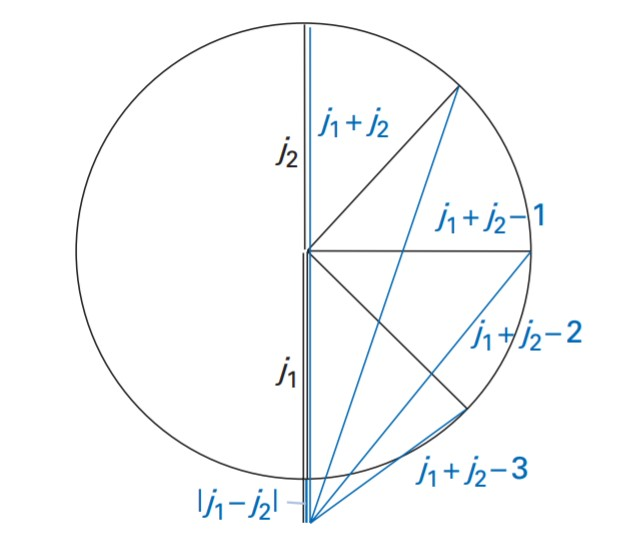
\includegraphics[width=6cm]{cgseries}
	\centering
	\caption{The allowed values of $j$ are just the third side of the triangle.}
	\label{fig:cgseries}
\end{figure}
\subsubsection{Relation between coupling schemes}
In \Cref{angmomcoup} we have introduced two pictures of coupling, the uncoupled 
and the coupled picture. Just as a recap, the uncoupled picture specifies the 
individual quantum numbers $j_i$ and $m_{ji}$. We usually use the \textbf{vector 
model of coupled angular momenta} to represent the differences between the two 
schemes, as in \Cref{fig:coupling}.
\begin{figure}[H]
	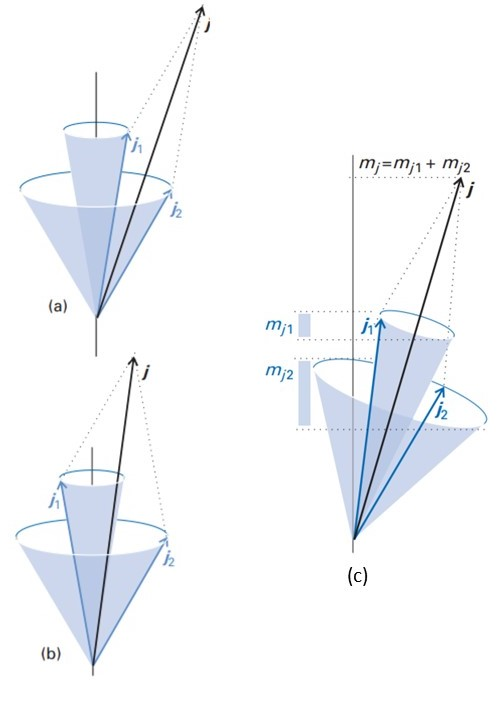
\includegraphics[width=6cm]{coupling}
	\centering
	\caption{(a) and (b) represent the uncoupled picture, in which we can't specify 
	$j_i$'s and $j$ simultaneously but can do so with $m_j$, as the $z$-component 
	is specified. (c) represents the coupled picture where the two $j_i$'s are 
	locked together, so $j$ (hence also $m_j$) is specified, but not the individual 
	components that add up to $m_j$.}
	\label{fig:coupling}
\end{figure}
We are more interested in the coupled picture as it gives us more immediate 
information of the system total parameters, as we shall see in 
\Cref{acc_for_spin}. So we should develop a way to quickly transform between the 
two pictures: the state $|j_1j_2;jm_j\rgl$ is built from a linear combination of 
all states with $m_{j1}+m_{j2}=m_j$:
\begin{equation}
\label{cgcoeffdef}
|j_1j_2;jm_j\rgl=\sum_{m_{j1},m_{j2}}C(m_{j1},m_{j2})|j_1m_{j_1};j_2m_{j2}\rgl,
\end{equation}
where the coefficients $C(m_{j1},m_{j2})$ are called \textbf{Clebsch-Gordan 
coefficients}, or vector coupling coefficients. For our case, $m_{j1}=m_{j2}=1/2$, 
the coefficients are easily seen to agree with our earlier efforts at establishing 
the singlet and triplet states. Omitting $j_1j_2$ in the notation and simply writing $|j,m_j\rgl$ or more specifically, $|S,M_S\rgl$, we have
\begin{equation}
\begin{aligned}
&|1,+1\rgl=\alpha_1\alpha_2\\
&|1,0\rgl=\frac{1}{\sqrt{2}}\alpha_1\beta_2+\frac{1}{\sqrt{2}}\beta_1\alpha_2\\
&|1,-1\rgl=\beta_1\beta_2\\
&|0,0\rgl=\frac{1}{\sqrt{2}}\alpha_1\beta_2-\frac{1}{\sqrt{2}}\beta_1\alpha_2. 
\end{aligned}
\end{equation}
The Clebsch-Gordan coefficients can be calculated as overlap integrals between 
the coupled and uncoupled states. We do so by right-multiplying \Cref{cgcoeffdef} 
by $\lgl j_1m'_{j1};j_2m'_{j2}|$:
\begin{equation}
\lgl j_1m'_{j1};j_2m'_{j2}|j_1j_2;jm_j\rgl=C(m'_{j1},m'_{j2}), 
\end{equation}
where other terms in the sum vanishes by the orthogonality of the states. This 
can be intuitively understood as how much the coupled state resembles the 
uncoupled state, or `how much' of the uncoupled state should be in the linear 
combination. For example, the state $|1,+1\rgl$ must be composed of $\alpha_1\alpha_2$ only as this is the only state with $M_S=+1$. 
\subsubsection{Atomic term symbols}
\label{term_symbols}
\hl{read chap 7 of atkins, and section on spin in B field in griffiths, priority: high. After that, re-write this section}
Term symbols give better descriptions than electron configurations, as we will see, same electronic configuration will give rise to different energies as a 
result of electrostatic interactions. The idea is to determine the total orbital 
angular momentum $\bvec{L}$ and the total spin angular momentum $\bvec{S}$ and 
then adding them vectorially to get the total angular momentum $\bvec{J}$:
\begin{equation}
\bvec{J}=\bvec{L}+\bvec{S}=\sum_i l_i+\sum_j s_j.
\end{equation}
This is called the \textbf{Russell-Saunders coupling} or \textbf{LS coupling}, 
which is only predominant in lighter ($Z<30$) atoms. \hl{same as spin-orbit coupling?}
The result of this sum is summarised as a \textbf{term symbol}, like
\begin{equation}
^{2S+1}L_J,
\end{equation}
where $L,S,J$ are the total orbital/total spin/total angular momentum quantum numbers, and $2S+1$ is known as the spin multiplicity. \\
With an argument exactly like the one given in \Cref{perm_totmom}, we can show 
that $\bvec{J}$ and $\bvec{S}$ are angular momenta and their values must run 
through integers and/or half integers. And since individual orbital angular 
momenta must be integers and individual spins can be both, so do the total. 
And another argument as in \Cref{perm_totmom} will give us that $J$ runs from 
$L+S$ to $|L-S|$. To summarise, the allowed values for the quantum numbers 
involved in the term symbol are
\begin{prt}[Term symbol]
The term symbol is
\begin{equation}
^{2S+1}L_J,
\end{equation}
where the allowed values are
\begin{equation}
\begin{aligned}
&S=0,1/2,1,3/2,\cdots\\
&(2S+1)=1,2,3,4,\cdots\\
&L=0,1,2,3,\cdots\\
&J=L+S,L+S-1,\cdots,|L-S|.
\end{aligned}
\end{equation}
\end{prt}
In analogy to assigning $s,p,d,f,\cdots$ to $\ell=0,1,2,3,\cdots$, we assign
$S,P,D,F,\cdots$ for $L=0,1,2,3,\cdots$. \\
Recall that the $z$-components of angular momenta simply add, \ie
\begin{equation}
\begin{aligned}
&L_z=\sum_i l_{zi}=\sum_i m_{li}=M_L\\
&S_z=\sum_i s_{zi}=\sum_i m_{si}=M_S
\end{aligned}
\end{equation}
The $M_S$ quantum number gives rise the $2S+1$ multiplicity (their energy will only be further split into levels in presence of external field \hl{todo: read up relevant stuff, reference, priority: low}). We will now look at a few examples. \\
\ \\
\textbf{Example 1: $ns^2$}
\begin{itemize}
	\item $s$ orbital means $\ell=0$, so $m_{li}=0$, and $M_L=0$, and this being the only allowed value of $M_L$ means $L=0$ or the S-state.
	\item The two spins must be antiparallel, so $M_S$ is also equal $0$, and so similarly $S=0$.
	\item By the same token, $J$ can also only be $0$.
	\item Therefore, the term symbol for $ns^2$ is $^1S_0$.
\end{itemize}
\textbf{Example 2: $np^6$}
\begin{itemize}
	\item $p$ orbital means $\ell=1$, so $m_{li}=-1,0,1$ so $M_L$ being the sum of all occupied orbitals (which is all of them) is $0$.
	\item Spins also all pair up to give $M_S=0$.
	\item Therefore $J$ can only be $0$
	\item The term symbol for $np^6$, and actually for \textbf{all} fully filled orbitals subshells, is $^1S_0$. It's also called \textbf{singlet S zero}.
\end{itemize}
\textbf{Example 3: }$ns^1n's^1$ (first excited state of Helium)
\begin{itemize}
	\item $M_L$ can only be zero as $m_{li}=0$.
	\item However now the spins are not confined to have antiparallel spins, and can independently take on values of $\pm1/2$, so $M_S$ can be $-1,0,1$. This means the largest value of $S$ is $1$ since that's the largest value $M_S$ can take on. So we must have $S=0,1$, corresponding to $^3S$ (triplet) and $^1S$ (singlet) states.
\end{itemize}
We list the possible states below:
\begin{center}
\begin{tabular}{c|c c c}
&\multicolumn{3}{c}{$M_S$}\\
$M_L$&$1$&$0$&$-1$\\
\hline
$0$&$0^+,0^+$&$0^+,0^-;0^-,0^+$&$0^-,0^-$
\end{tabular}
\end{center}
where $0^+$ means $m_l=0$ and $m_s=+1/2$ and vice versa. The middle two states are 
not indistinguishable because the spatial orbitals are not the same ($1s$ and 
$2s$)There are $4$ \textbf{microstates}. The triplet state accounts for one state 
from each column, and the singlet state must claim the remaining $M_S$ state, and 
it doesn't matter which one each state takes. \par
And we are left with $J$ to determine. We add $M_L$ and $M_S$ to get $M_J$. 
For the triplet state $M_J$, $M_J=1,0,-1$, so $J=1$. For the singlet state 
similarly $J=0$.\par
Therefore the two term symbols the configuration $ns^1n's^1$ correspond to are $^3S_1$ and $^1S_0$. \\
\ \\
\textbf{Example 4: }Carbon atom\\
\ \\
As shown previously, we do not need to worry about fully filled subshells and only need to focus on $2p^2$. Let's derive a general result first: 
\begin{lemma}[Number of electron assignments]
For $G$ number of \textbf{equivalent} (same subshell) spin-orbitals and $N$ 
electrons, which are indistinguishable, the number of ways to 
assign the electrons, $D(G,N)$ is 
\begin{equation}
D(G,N)=\frac{G!}{N!(G-N)!}.
\end{equation}
\end{lemma}
So for carbon, we have $15$ ways to assign the electrons. Intuitively, the first electron can take any of the $6$ spin-orbitals, the second can take the remaining 
$5$, and a factor of $2!$ is divided through for they are indistinguishable, 
giving a total of $15$ ways to arrange. \par
To find all these $15$ microstates we again use a table. But before that we need 
to find out the values of $M_L$ and $M_S$. It's easily seen that $M_L$ runs from 
$-2$ to $+2$ and $M_S$ from $-1$ to $+1$. So $L=0,1,2$ and $S=0,1$. The table is then 
\begin{center}
\begin{tabular}{c|c c c}
&\multicolumn{3}{c}{$M_S$}\\
$M_L$&$1$&$0$&$-1$\\
\hline
$2$&\highlight{1^+,1^+}&$1^+,1^-$&\highlight{1^-,1^-}\\
$1$&$0^+,1^+$&$1^+,0^-;1^-,0^+$&$0^-,1^-$\\
$0$&\highlight{0^+,0^+}$;1^+,-1^+$&$1^+,-1^-;-1^+,1^-;0^+,0^-$&$1^-,-1^-;$\highlight{0^-,0^-}\\
$-1$&$0^+,-1^+$&$0^+,-1^-;0^-,-1^+$&$0^-,-1^-$\\
$-2$&\highlight{-1^+,-1^+}&$-1^+,-1^-$&\highlight{-1^-,-1^-}
\end{tabular}
\end{center}
where we make no distinction like the previous case between $1^+,0^-$ and 
$0^-,1^+$ because the spatial orbitals are equivalent now. The grey terms are 
forbidden by the Pauli exclusion principle. We now assign term symbols to the 
microstates. \par
We start by remarking that although the \textbf{allowed} values of 
$L$ and $S$ is $0$ to $2$ and $0$ to $1$ respectively, the actual \textbf{permitted} term symbols are not necessarily all possible permutations of these values. For example, the largest value of $M_L$ is $2$ and it only occurs with $M_S=0$, this means that $L=2$ state only occurs with $S=0$. For the remaining states, the largest $M_L=1$, and it occurs with all three $M_S$ values, hence there must be a state with $L=1$ and $S=1$. We list the term symbols below:
\begin{itemize}
	\item $L=2$, $S=0$, \ie $^1D$: one state per row in the $M_S=0$ column. $J$ can only take up one value, which is $2$. The complete term symbol is $^1D_2$.
	\item $L=1$, $S=1$, \ie $^1P$: nine states per remaining cells. $J$ can take up values from $2$ to $0$, so complete term symbols are $^3P_2$, $^3P_1$, and $^3P_0$.\footnote{Another way to look at this is that the nine states correspond to $M_J$ of $2,1,1,0,0,-1,0,-1,-2$, so we can isolate three sets of $M_J$ running from $-J$ to $J$ with $J=0,1,2$ respectively.}
	\item $L=0$, $S=0$, term symbol $^1S_0$, naturally.
\end{itemize}
As can be seen, we don't really have to specify $J$ as it can be deduced from $S$ and $L$. The degeneracies of each state is given by $2J+1$. \par
At last, we can introduce Hund's rules, \hl{todo: theoretical foundations, priority: medium}:
\begin{thrm}[Hund's rules]
The three Hund's rules state that
\begin{enumerate}
	\item The state with the largest value of $S$ is the most stable (has the lowest energy), and stability decreases with decreasing $S$. 
	\item For states with the same value of $S$, the state with the largest value of $L$ is the most stable. 
	\item If the states have the same value of $L$ and $S$, then, for a subshell that is less than half filled, the state with the smallest value of $J$ is the most stable; for a subshell that is more than half filled, the state with the largest value of $J$ is the most stable. 
\end{enumerate}
\end{thrm}
\subsubsection{Molecular term symbols}
The following discussion only strictly applies to homonuclear diatomics, for which only the orbital angular momentum along the internucalear axis is defined.\par
The molecular term symbol is given in the form of 
\begin{equation}
	^{2\Sigma+1}\Lambda^{\pm}_{g/u},
\end{equation}
$\Sigma$ is just the spin angular momentum, effectively the half the number of unpaired electrons in the molecule.\par
$\Lambda$ is the orbital angular momentum \emph{along the internuclear axis}, given as
\begin{equation}
	\Lambda=\sum_i M_{L,i},
\end{equation}
with \emph{unpaired} electrons in $\sigma$ orbitals having $M_L=0$ and those in $\pi$ orbitals having $M_L=1$ and so on.\par
The $g/u$ labels denotes the \emph{inversion symmetry}, where the overall inversion symmetry is a direct product of the inversion symmetry of all occupied orbitals, with 
\begin{equation}
	g\times g=g\ \ u\times u=g\ \ g\times u=u\ \ u\times g=u.
\end{equation}
And finally the $\pm$ label denotes the \emph{mirror-plane} symmtry, where the mirror plane contains the internuclear axis, where $+$ means unchanged upon reflection and $-$ means the sign changes upon reflection. 
Mathematically speaking, reflection changes the sign of $\phi$. Let's see this in action\hl{draw diagram}, say we have the ground state of oxygen, which has an electronic configuration of $\pi^2$, which has two orbitals with $M_L=\pm 1$, which leads to two $^1\Delta$ states with two electrons in either orbitals, and a $^3\Sigma$ and $^1\Sigma$ state with two electrons in both states but two orientations. The wavefunctions for the two orbitals are
\begin{equation}
\begin{aligned}
	\pi_+&=F(\bvec{r_a},\bvec{r_b})e^{i\phi}\\
	\pi_-&=F(\bvec{r_a},\bvec{r_b})e^{-i\phi}
\end{aligned}
\end{equation}
we further define the reflection operator
\begin{equation}
	\sigma_{xy}\pi_{\pm}=\pi_{\mp}
\end{equation}
and the total wavefunction for the two electrons
\begin{equation}
	\Psi(\bvec{r_1},\bvec{r_2})=\frac{1}{\sqrt{2}}[\pi_+(1)\pi_-(2)\mp\pi_-(1)\pi_+(2)]\times\bvec{\sigma}_{\pm}
\end{equation}
where the top sign denotes triplet, whose spin wavefunction is symmetric to exchange, and the bottom sign denotes singlet. Now the action of the total reflection operator $\sigma_{\text{tot}}=\sigma_{xy}(1)\sigma_{xy}(2)$ is
\begin{equation}
\begin{aligned}
	\sigma_{\text{tot}}\Psi(\bvec{r_1},\bvec{r_2})&=\frac{1}{\sqrt{2}}\sigma_{xy}(1)\sigma_{xy}(2)[\pi_+(1)\pi_-(2)\mp\pi_-(1)\pi_+(2)]\times\bvec{\sigma}_{\pm}\\
	&=\frac{1}{\sqrt{2}}[\pi_-(1)\pi_+(2)\mp\pi_+(1)\pi_-(2)]\times\bvec{\sigma}_{\pm}\\
	&=\mp\Psi(\bvec{r_1},\bvec{r_2})
\end{aligned}
\end{equation}
therefore we see that the final full term symbols are $^3\Sigma^-$ and $^1\Sigma^+$. \par
This is only going to matter in $\Lambda=0$ ($\Sigma$) states, this is because all other states have a two-fold degeneracy, so the reflection operation is just going to interchange them, whereas in $\Sigma$ states there's no degeneracy.\par
\textbf{More exmamples}\par
$1\sigma^1\ 2\sigma^1$\\
As the electrons don't occupy the same orbitals, Pauli exclusion principle doesn't apply anyway, and also, since $\sigma$ MOs have no $\phi$ dependence, it has to be unchanged upon reflection, therefore $^1\Sigma^+$ and $^3\Sigma^+$ are produced.\par
$\sigma^1$\\
Similar argument produces $^2\Sigma^+$.\par
Closed shell\\
Close shells must have $S=0$ which forces the singlet configuration, which means antisymmetric spin wavefunction and hence $^1\Sigma^+$.\par
$\pi^1$\\
This simply produces $^2\Pi$, specifying the signs is unnecessary as the term is 2-degenerate anyway.

\section{Identical particles}
\subsection{Two particle systems}
\subsubsection{The \sch}
The state of a two-particle system is a function of both particle's coordinates 
and time:
\begin{equation}
\ups(\bvec{r_1},\bvec{r_2},t).
\end{equation}
Its time evolution is, as always, determined by the \sch
\begin{equation}
i\hbar\diffp{\ups}{t}=H\ups, 
\end{equation}
where the Hamiltonian is 
\begin{equation}
H=-\frac{\hbar^2}{2m_1}\onabla_1^2-\frac{\hbar^2}{2m_2}\onabla_2^2+V(\bvec{r_1},\bvec{r_2},t)
\end{equation}
The probability of finding particle $1$ in $d^3\bvec{r_1}$ and 
particle $2$ in $d^3\bvec{r_2}$ is
\begin{equation}
|\ups(\bvec{r_1},\bvec{r_2},t)|^2d^3\bvec{r_1}d^3\bvec{r_2}. 
\end{equation}
The normalisation requirement is therefore
\begin{equation}
\int|\ups(\bvec{r_1},\bvec{r_2},t)|^2d^3\bvec{r_1}d^3\bvec{r_2}=1.
\end{equation}
For \textbf{time-independent} potentials, we can use the usual separation of 
variables:
\begin{equation}
\ups(\bvec{r_1},\bvec{r_2},t)=\psi(\bvec{r_1},\bvec{r_2})e^{-iEt/\hbar}, 
\end{equation}
where $\psi$ is such that
\begin{equation}
H\psi=E\psi.
\end{equation}
\subsubsection{Centre-of-mass coordinates}
If, in a \textbf{two particle system}, where the potential depends only on 
$\bvec{r}\equiv\bvec{r_1}-\bvec{r_2}$ between the two particles, we can use the 
centre-of-mass coordinates to simplify and \textit{separate} the \sch as follows: 
we define the \textbf{centre-of-mass coordinate}:
\begin{equation}
\bvec{R}\equiv\frac{m_1\bvec{r_1}+m_2\bvec{r_2}}{m_1+m_2}
\end{equation}
Now, we need to re-write the \sch in terms of the new coordinates, 
and first of all we need to write out the Hamiltonians, which is fiddly to do: 
we first need to see that 
\begin{equation}
\onabla_1f=\diffp{f}{r_{1_x}}+\diffp{f}{r_{1_y}}+\diffp{f}{r_{1_z}}.
\end{equation}
So to re-write it, we note that $r_{1_x}$ is only dependent on $r_x$ and $R_x$, 
and so on, so
\begin{equation}
\label{fr1x}
\begin{aligned}
\diffp{f}{r_{1_x}}&=\diffp{f}{r_x}\diffp{r_x}{r_{1_x}}+\diffp{f}{R_x}\diffp{R_x}{r_{1_x}}\\
&=\diffp{f}{r_x}+\diffp{f}{R_x}\frac{\mu}{m_2}, 
\end{aligned}
\end{equation}
and
\begin{equation}
\begin{aligned}
\diffp{f}{r_{2_x}}&=\diffp{f}{r_x}\diffp{r_x}{r_{2_x}}+\diffp{f}{R_x}\diffp{R_x}{r_{2_x}}\\
&=-\diffp{f}{r_x}+\diffp{f}{R_x}\frac{\mu}{m_1}, 
\end{aligned}
\end{equation}
and so on for other components, so
\begin{subequations}
\begin{align}
&\onabla_1=\onabla_r+\frac{\mu}{m_2}\onabla_R\\
&\onabla_2=-\onabla_r+\frac{\mu}{m_1}\onabla_R.
\end{align}
\end{subequations}
To get the Laplacian, we note that it's not equivalent to left multiplying 
the transformed nabla operator twice, but instead we have to go 
back to \Cref{fr1x}, and differentiating it again wrt $r_{1_x}$ and so on:
\begin{equation}
\begin{aligned}
\diffp[2]{f}{r_{1_x}}&=\lf(-\diffp{}{r_x}+\frac{\mu}{m_2}\diffp{}{R_x}\rt)\lf(-\diffp{f}{r_x}+\diffp{f}{R_x}\frac{\mu}{m_2}\rt)\\
&=\diffp[2]{f}{r_x}-\diffp{f}{r_x,R_x}\frac{2\mu}{m_2}+\diffp[2]{f}{R_x}\lf(\frac{\mu}{m_2}\rt)^2,
\end{aligned}
\end{equation}
and 
\begin{equation}
\begin{aligned}
\diffp[2]{f}{r_{2_x}}&=\lf(\diffp{}{r_x}+\frac{\mu}{m_1}\diffp{}{R_x}\rt)\lf(\diffp{f}{r_x}+\diffp{f}{R_x}\frac{\mu}{m_1}\rt)\\
&=\diffp[2]{f}{r_x}-\diffp{f}{r_x,R_x}\frac{2\mu}{m_1}+\diffp[2]{f}{R_x}\lf(\frac{\mu}{m_1}\rt)^2,
\end{aligned}
\end{equation}
so we have
\begin{equation}
-\frac{\hbar^2}{2m_1}\onabla^2_1=-\frac{\hbar^2}{2m_1}\onabla_r^2-\onabla^2_R\frac{\hbar^2\mu^2}{m_1m_2^2}-(\text{mixed partial term})
\end{equation}
and 
\begin{equation}
-\frac{\hbar^2}{2m_1}\onabla^2_2=-\frac{\hbar^2}{2m_2}\onabla_r^2-\onabla^2_R\frac{\hbar^2\mu^2}{m_2m_1^2}+(\text{same mixed partial term}).
\end{equation}
Finally, the \sch is 
\begin{equation}
\lf[-\frac{\hbar^2}{2(m_1+m_2)}\onabla^2_R-\frac{\hbar^2}{2\mu}\onabla^2_r+V(\bvec{r})\rt]\psi=E\psi. 
\end{equation}
We attempt separation of variables:
\begin{equation}
\psi(\bvec{R},\bvec{r})=\psi_R(\bvec{R})\psi_r(\bvec{r}),
\end{equation}
and we obtain two equations:
\begin{subequations}
\begin{align}
-\frac{\hbar^2}{2(m_1+m_2)}\onabla^2_R\psi_R&=E_R\psi_R\\
\lf[-\frac{\hbar^2}{2\mu}\onabla_r^2+V(\bvec{r})\rt]\psi_r&=E_r\psi_r.
\end{align}
\end{subequations}
This is saying that we have successfully decoupled the equation into two 
independent systems: the total mass ($m_1+m_2$), moving as a 
free particle ($0$ potential) and the relative motion as a 
single particle with reduced mass subject to potential $V$. 
\subsubsection{Bosons and fermions}
Suppose we now have a two particle system that is non-interacting, which is to 
say that the two particles are in their own one-particle states and that they 
are independent - this is by no means always true, as in the singlet spin 
configuration where two spins are correlated - we can write
\begin{equation}
\psi(\bvec{r}_1,\bvec{r}_2)=\psi_a(\bvec{r}_1)\psi_b(\bvec{r}_2).
\end{equation}
In writing this we have presumed that the two particles are 
\textbf{distinguishable}, otherwise the labels $a$ and $b$ wouldn't make any 
sense. However, almost all the particles we will be dealing with will 
\textit{not} be distinguishable. Therefore, the most we can say its that 
\textit{one} particle is in state $a$ and the other in state $b$. 
We note that since they are insdistinguishable, the exchange of labels 
\textit{must} have no effect on the probability density, \ie
\begin{equation}
|\psi(1,2)|^2=|\psi(2,1)|^2,\ \imp\ \psi(1,2)=\pm\psi(2,1).
\end{equation}
So this means we can write
\begin{equation}
\psi_{\pm}(\bvec{r}_1,\bvec{r}_2)=A[\psi_a(\bvec{r}_1)\psi_b(\bvec{r}_2)\pm\psi_b(\bvec{r}_1)\psi_a(\bvec{r}_2)]. 
\end{equation}
This wavefunction is \textit{non-committal} as to which particle is in which 
state, but when do we use which sign? We introduce the postulate
\begin{post}[Bosons and fermions]
\ \\
All particles with \textit{integer} spins are bosons, and\\
all particles with \textit{half integer} spins are fermions. \\
We use the \textit{plus sign} for bosons and \textit{minus sign} for fermions. 
\end{post}
It then follows that 
\begin{thrm}[Pauli exclusion principle]
Two identical fermions, for example, two electrons, cannot occupy the same state, 
for if $\psi_a=\psi_b$, then 
\begin{equation}
\psi_-(\bvec{r}_1,\bvec{r}_2)=A[\psi_a(\bvec{r}_1)\psi_a(\bvec{r}_2)-\psi_a(\bvec{r}_1)\psi_a(\bvec{r}_2)]=0,
\end{equation}
and we are left with no wavefunction at all. 
\end{thrm}
A more general re-formulation of problem requires the introduction of 
the \textbf{exchange operator}:
\begin{defi}[Exchange operator]
The exchange operators is defined as 
\begin{equation}
Pf(\bvec{r}_1,\bvec{r}_2)=f(\bvec{r}_2,\bvec{r}_1). 
\end{equation}
\end{defi}
\begin{defi}[Properties of the exchange operator]
\ \\
(1) It is immediately clear that
\begin{equation}
P^2=I.
\end{equation}
(2) And therefore the eigenvalues of $P$ are $\pm1$. \\
(3) If we have two \textit{identical} particles, the Hamiltonian must treat them the 
same way: $m_1=m_2$ and $V(\bvec{r}_1,\bvec{r}_2)=V(\bvec{r}_2,\bvec{r}_1)$, therefore $P$ and $H$ are compatible observables: 
\begin{equation}
[P,H]=0.
\end{equation}
\end{defi}
\begin{thrm}[Symmetrisation requirement]
\label{sym_req}
Because $P$ and $H$ commute, we can find simultaneous eigenstates of both, \ie 
we can find solutions to \sch that are either symmetric (eigenvalue $+1$) or 
antisymmetric (eigenvalue $-1$) under excahnge of labels:
\begin{equation}
\psi(\bvec{r}_1,\bvec{r}_2)=\pm\psi(\bvec{r}_2,\bvec{r}_1). 
\end{equation}
Therefore, if a system begins in a state it must remain in this state. 
The plus sign is for bosons and negative for fermions.
\end{thrm}
\subsubsection{Exchange forces}
We examine a 1D example. Let's suppose one particle is in $\psi_a(x)$ and another in $\psi_b(x)$, 
and these two states are orthogonal and normalised. \textit{If} the two particles 
are distinguishable, and number $1$ is the one in state $\psi_a$, then the 
composite wavefunction is 
\begin{equation}
\label{comp_dist}
\psi(x_1,x_2)=\psi_a(x_1)\psi_b(x_2).
\end{equation}
If they are identical bosons or fermions, the composite will be 
\begin{equation}
\label{comp_iden}
\psi_{\pm}(x_1,x_2)=\frac{1}{\sqrt{2}}[\psi_a(x_1)\psi_b(x_2)\pm\psi_b(x_1)\psi_a(x_2)].
\end{equation}
Let's calculate the expectation value of the square of the separation distance 
between the two particles, given by
\begin{equation}
\lgl (x_1-x_2)^2\rgl=\lgl x_1^2\rgl+\lgl x_2^2\rgl-2 \lgl x_1x_2\rgl. 
\end{equation}
\textbf{Case 1: Distinguishable particles}\\
We use the wavefunction in \Cref{comp_dist}:
\begin{equation}
\lgl x_1\rgl=\int x_1^2|\psi_a(x_1)|^2\dx_1\int|\psi_b(x_2)|^2\dx_2=\lgl x^2\rgl_a, 
\end{equation}
(the expectation of $x^2$ in the \textit{one-particle} state $\psi_a$) so similarly 
\begin{equation}
\lgl x_2^2\rgl=\lgl x_2^2\rgl_b. 
\end{equation}
And
\begin{equation}
\lgl x_1x_2\rgl=\int x_1|\psi_a(x_1)|^2\dx_1\int x_2|\psi_b(x_2)|^2\dx_2=\lgl x\rgl_a \lgl x\rgl_b.
\end{equation}
Collecting, we have
\begin{equation}
\label{delx_dist}
\lgl (x_1-x_2)^2\rgl=\lgl x^2\rgl_a+\lgl x^2\rgl_b-2 \lgl x\rgl_a \lgl x\rgl_b.
\end{equation}
\textbf{Case 2: Identical particles}\\
We now have to use the wavefunctions in \Cref{comp_iden}:
\begin{equation}
\begin{aligned}
\lgl x_1^2\rgl=&\frac{1}{2}\lf[\int x_1^2|\psi_a(x_1)|^2\dx_1\int|\psi_b(x_2)|^2\dx_2\rt.\\
&+\int x_1^2|\psi_b(x_1)|^2\dx_1\int|\psi_a(x_2)|^2\dx_2\\
&\pm\int x_1^2\psi_a(x_1)^*\psi_b(x_1)\dx_1\int\psi_b(x_2)^*\psi_a(x_2)\dx_2\\
&\lf.\pm \int x_1^2\psi_b(x_1)^*\psi_a(x_1)\dx_1\int\psi_a(x_2)^*\psi_b(x_2)\dx_2\rt]\\
=&\frac{1}{2}\lf[\lgl x^2\rgl_a+\lgl x^2\rgl_b\pm0\pm0 \rt]\\
=&\frac{1}{2}\lf(\lgl x^2\rgl_a+\lgl x^2\rgl_b\rt).
\end{aligned}
\end{equation}
And likewise
\begin{equation}
\lgl x_2^2\rgl=\frac{1}{2}\lf(\lgl x^2\rgl_b+\lgl x^2\rgl_a\rt).
\end{equation}
We observe that 
\begin{equation}
\lgl x_1^2\rgl=\lgl x_2^2\rgl
\end{equation}
since we can't tell them apart. Now
\begin{equation}
\begin{aligned}
\lgl x_1x_2\rgl=&\frac{1}{2}\lf[\int x_1|\psi_a(x_1)|^2\dx_1\int x_2|\psi_b(x_2)|^2\dx_2\rt.\\
&+\int x_1|\psi_b(x_1)|^2\dx_1\int x_2|\psi_a(x_2)|^2\dx_2\\
&\pm\int x_1\psi_a(x_1)^*\psi_b(x_1)\dx_1\int x_2\psi_b(x_2)^*\psi_a(x_2)\dx_2\\
&\lf.\pm\int x_1\psi_b(x_1)^*\psi_a(x_1)\dx_1\int x_2\psi_a(x_2)^*\psi_b(x_2)\dx_2 \rt]\\
=&\frac{1}{2}\lf(\lgl x\rgl_a \lgl x\rgl_b+\lgl x\rgl_b \lgl x\rgl_a\pm\lgl x\rgl_{ab} \lgl x\rgl_{ba}\pm \lgl x\rgl_{ba} \lgl x\rgl_{ab} \rt)\\
=&\lgl x\rgl_{a} \lgl x\rgl_{b}\pm|\lgl x\rgl_ab|^2, 
\end{aligned}
\end{equation}
where 
\begin{equation}
\lgl x\rgl_{ab}\equiv\int x\psi_a(x)^*\psi_b(x)\dx.
\end{equation}
Collecting we have
\begin{equation}
\label{delx_iden}
\lgl (x_1-x_2)^2\rgl_{\pm}=\lgl x^2\rgl_a+\lgl x^2\rgl_b-2 \lgl x\rgl_a \lgl x\rgl_b\mp2 |\lgl x\rgl_{ab}|^2.
\end{equation}
\begin{thrm}[Exchange force]
\ \\
By comparing \Cref{delx_dist} and \Cref{delx_iden}, we see that the difference 
lies in the final term:
\begin{equation}
\lgl (\Delta x)^2\rgl_{\pm}=\lgl (\Delta x)^2\rgl_d\mp2 |\lgl x\rgl_{ab}|^2,
\end{equation}
where the subscript $d$ stands for `distinguishable'. 
Therefore we can see that identical bosons are closer together and identical 
fermions further apart than distinguishable particles in the same two states. 
Notice that $\lgl x\rgl_{ab}$ \textbf{vanishes} unless the two wavefunctions 
\textbf{overlap}. Therefore, it is acceptable to treat electrons with 
non-overlapping wavefunctions as distinguishable. The increase or decrease 
in between identical particles are called an \textbf{exchange force}.
\end{thrm}
We now take a look at the hydrogen molecule, H$_2$. To a good approximation
\footnote{See next section.}, the ground state consists of one electron in the 
hydrogen atom ground state centred around nucleus $1$ and another around nucleus 
$2$. If electrons were bosons, the exchange force would concentrate the electrons 
towards the middle of the internuclear space, and as a result pull the protons 
inward, accounting for the covalent bond. However, electrons are fermions, and 
that would mean the concentration of negative charge should be on the wings, 
tearing the molecule apart. This is obviously wrong, and we are reminded that 
we have been ignoring spins all this while - the symmetrisation requirement 
(\Cref{sym_req}) requires that the \textbf{complete wavefunctions} of fermions be 
antisymmetric, not just the spatial wavefunctions. The complete wavefunctions of 
electrons are
\begin{equation}
\psi_e(\bvec{r},\bvec{s})=\psi(\bvec{r})\chi(\bvec{s}).
\end{equation}
This is assuming that the spin and the spatial wavefunction are 
\textit{uncoupled}, therefore separable. Under the same assumption, we can write 
the two-electron state as
\begin{equation}
\psi_{2e}(\bvec{r}_1,\bvec{r}_2,\bvec{s}_1,\bvec{s}_2)=\psi_{\pm}(\bvec{r}_1,\bvec{r}_2)\chi(\bvec{s}_1,\bvec{s}_2), 
\end{equation}
where $\chi(\bvec{s}_1,\bvec{s}_2)$ can be one of the four (three triplet one 
singlet) states in \Cref{add_moment}. Now, we must require bonding, therefore 
symmetric\footnote{Remember that the exchange force favours bonding as long as the 
\textit{spatial} wavefunction is symmetric, and it makes no use of the spinor as 
the `integration' of orthonormal spinors always return the Kronecker delta.}, \textit{spatial} wavefunctions. 
We remember that the singlet state is antisymmetric\footnote{We can actually 
derive this from symmetry requirements alone, stating from the four possible 
combinations and then consider their coefficients as in \cite{spincoeff}.}, therefore the spatial 
wavefunction of the electron that's multiplied to it can (and must) be symmetric. 
This can be confusing because we appear to have just derived that all 
electron wavefunctions must be antisymmetric. But in fact we have not, 
\Cref{sym_req} only requires that the complete wavefunction be accordingly 
symmetrised, not spatial or spinor parts separately. \par
Therefore, we have now shown that the bonding orbital will have electrons occupy 
the singlet configuration, with total spin zero, and the antibonding orbital one of the triplet configurations. \par
Another more elementary but more intuitive way to look at this is that electrons 
with the same spin cannot be found at the same spot and the electron density will be low around another electron with the same spin. This is not the case for electrons with opposite spin. Because of the Coulombic repulsion, electrons with like spins are lower in energy than those with opposite spin. This explains in part the Hund's rule. Also, the triplet state is more stable than the singlet state, however the latter is essential for chemical bonding to happen, and bonding happens because the lowering in energy more than compensates for the exchange force. 
\chapter{Spectroscopy}
\section{Atomic spectroscopy}
\subsection{Selection rules}
\begin{thrm}[The Laporte selection rule]
The Laporte selection rule states that electric dipole transition that does not involve a change in parity is strictly forbidden, while those involving a change in parity may be allowed. In other words, the only transitions allowed are those involving a change in parity.
\end{thrm}
\begin{proof}
The transition probability between two states are given by the Einstein `B' coefficient which is given in \cref{einsteincoeff}, which is proportional to the modulus squaured of the \emph{transition dipole moment}
\begin{equation}
	\bvec{\mu}_{i\rightarrow f}=\lgl i | \uvec{\mu} |f\rgl
\end{equation}
\Cref{zerointegral} tells that the integrand must contain the tot. sym. irrep of the group the particle belongs to, which in this case is the full rotation group $R_3$. The inversion operation\footnote{Just because we can readily deduce the parity from the orbital angular momentum. In principle any other operation is fine, we just need to see whether the direct product is $[1,1,\dots,1]$} is diagnostic: if the integrand is antisymmetrical wrt. inversion the integral is necessarily zero. \textbf{Parity} is just the $g/u$ label, but represented numerically as $\pm1$. The parity of atmoic orbitals is $(-1)^l$, because the dipole moment operator has $u$ symmetry, the overall parity of the integrand is
\begin{equation}
	(-1)^{l_i}(-1)(-1)^{l_f}
\end{equation}
which shows the two orbitals must have \emph{opposite parity} for the integral to be plausibly non-zero.
\end{proof}
This allows us to deduce the selection rule for orbital angular momentum of an atom
\begin{thrm}[Selection rule for orbital angular momentum]
The selection rule is 
\begin{equation}
	\Delta l=\pm1
\end{equation}
\end{thrm}
\begin{proof}
	As the dipole moment operator transforms like a translation which is exactly like $l=1$ spherical harmonics, the representative of $\uvec{\mu}$ is $\Gamma^{(1)} $. The overall direct product for $\lgl i | \uvec{\mu}|f \rgl $ is 
	\begin{equation}
	\begin{aligned}
		&\Gamma^{(l_i)}\otimes\Gamma^{(1)}\otimes\Gamma^{(l_f)}\\
		=&\lf(\Gamma^{(l_i+1)}\oplus\Gamma^{(l_i)}\oplus\Gamma^{(l_i-1)} \rt)\otimes\Gamma^{(l_f)}
	\end{aligned}
	\end{equation}
	The requirement is for the integrand to \emph{contain} the tot. sym. irrep, so clearly $\Gamma^{(l_f)}$ must be one of the three terms in front. And $\Delta l=0$ is Laporte forbidden so we are left with the selection rule of $\Delta l=\pm1$.
\end{proof}
The selection rule for $m_l$ can be deduced as well:
\begin{thrm}[Selection rule for magnetic quantum number]
The selection rule is
\begin{equation}
	\Delta m_l=0,\pm1
\end{equation}
\end{thrm}
\begin{proof}
	 We now just need to look at the $\phi$ dependence only, which gives us the integral of the form
\begin{equation}
	\int^{2\pi}_0e^{-im_{li}\phi}(\hat{\mu}_j)e^{im_{lf}\phi}\dif \phi
\end{equation}
with $\uvec{\mu}=-e\bvec{r}$ is the electric dipole operator, which in spherical coordinates is
\begin{equation}
	-er
	\begin{pmatrix}
		\sin\theta\cos\phi\\
		\sin\theta\sin\phi\\
		\cos\phi
	\end{pmatrix}
\end{equation}
Now considering radiation that is plane-polarised with the electric field in the $z$-direction, remembering the first bra represents the complex conjugate, we get
\begin{equation}
	\int^{2\pi}_0e^{-im_{lf}\phi}(-er\cos\theta)e^{im_{li}\phi}\dif \phi\propto\int^{2\pi}_0e^{i(m_{li}-m_{lf})\phi}\dif \phi
\end{equation}
which gives $\Delta m_l=0$. If the radiation is polarised in the $x$-direction, we have
\begin{equation}
\begin{aligned}
	&\int^{2\pi}_0e^{-im_{li}\phi}(-er\sin\theta\cos\phi)e^{im_{lf}\phi}\dif \phi\\
	\propto&\int^{2\pi}_0e^{-im_{li}\phi}(e^{i\phi}+e^{-i\phi})e^{im_{lf}\phi}\dif \phi\\
	=&\int^{2\pi}_0e^{i(m_{lf}-m_{li}+1)\phi}+e^{i(m_{lf}-m_{li}-1)\phi}\dif \phi
\end{aligned}
\end{equation}
which means, to have a non-zero result, $\Delta m_l=\pm1$. The $y$-polarised radiation gives the same result.
\end{proof}
\subsection{Fine structure}
Spectroscopy measures transitions between energy levels, for example photoelectron spectroscopy measures that between electronic levels, and IR and Raman spectroscopy measures that between vibrational levels, and NMR between nuclear spin levels. By the same token, the energy differences between electronic spin levels can also be measured, and we'll develop some theoretical treatments to elucidate the fine structure of atomic spectra.
\subsubsection{Orbital and spin magnetic moments}
\paragraph{Orbital magnetic moment}
The orbital magentic moment can be derived from classical arguments: the current ($\diff qt$) of a circulating electron in the $xy$-plane at speed $v$ at radius $r$ is
\begin{equation}
 	I=-\frac{ev}{2\pi r}
\end{equation} 
The magnetic dipole in the $z$-direction is
\begin{equation}
	m_z=IA=-\frac{ev}{2\pi r}\times\pi r^2=-\tfrac{1}{2}evr
\end{equation}
The $z$-component of the angular momentum is 
\begin{equation}
	l_z=m_{\mathrm{e}}vr
\end{equation}
so
\begin{equation}
	m_z=\underbrace{-\frac{e}{2m_{\mathrm{e}}}}_{\gamma_{\mathrm{e}}} l_z
\end{equation}
As the argument holds in all three cardinal directions, we arrive at the simple relation
\begin{equation}
	\bvec{m}=\gamma_{\mathrm{e}}\bvec{l}
\end{equation}
where $\gamma_{\mathrm{e}}=-e/2m_{\mathrm{e}}$ is called the \emph{gyromagnetic ratio} of the electron.\par
Now we're done with the classical and technically incorrect derivation, we need to introduce the quantum mechanical quantisation by claiming $m_z$ is quantised like $l_z$, namely
\begin{equation}
	m_z=\gamma_{\mathrm{e}}m_l\hbar,\ \ m_l=-l,-l+1,\dots,l
\end{equation}
and we can define the \emph{Bohr magneton} as $\mu_{\mathrm{B}}=-\gamma_{\mathrm{e}}\hbar=e\hbar/2m_{\mathrm{e}}$ so we can write
\begin{equation}
	m_z=-\mu_{\mathrm{B}}m_l,\ \ |m_l|=0,1,\dots,l
\end{equation}
\paragraph{Spin magnetic moment}
The orbital angular momentum has a classical analogue whereas the intrinsic spin does not. We can't rely on classical arguments here because there are none. It turns out that for the spin magnetic moment, 
\begin{equation}
\begin{aligned}
	&\bvec{m}=g_{\mathrm{e}}\gamma_{\mathrm{e}}\bvec{s},\ \ g_{\mathrm{e}}\approx2\\
	&m_z=-g_{\mathrm{e}}\mu_{\mathrm{B}}m_s,\ \ m_s=\pm\tfrac{1}{2}
\end{aligned}
\end{equation}
$g_{\mathrm{e}}$ is known as the \emph{$g$-factor}
\footnote{This is twice the expected value from claisscal mechanics. The full derivation of the factor requires the relativistic Dirac equation and even then a much smaller (0.00232) correction requires quantum electrodynamics. One interesting way to think about this is that the quantum mechanical rotation operator will return $\text{Rot}(2\pi)|\chi\rgl=-|\chi\rgl$, which in essence says that \emph{a full rotation in quantum mechanics is $4\pi$ radian instead of $2\pi$}! So the velocity of rotation and so on are all doubled.}.
The nuclear spin magentic moment obeys the same rule:
\begin{equation}
\begin{aligned}
	&\bvec{m}=g_{\mathrm{I}}\gamma_{\mathrm{N}}\bvec{I}\\
	&m_z=g_{\mathrm{I}}\mu_{\mathrm{N}}m_I,\ \ m_s=-I,-I+1,\dots,I
\end{aligned}
\end{equation}
where $\mu_{\mathrm{N}}=e\hbar/2m_{\mathrm{p}}$ is the \emph{nuclear magneton}, and $g_{\mathrm{I}}$ is the nuclear magneton, of order $10^0$.
\paragraph{Land{\'e} $g$-factor}
For an electron with both orbital and spin magnetic moment, the resultant magnetic moment is given exactly\footnote{The only approximation being, $g_{\mathrm{e}}=2$ which goes into the `offset' constant in front.} as
\begin{equation}
	\bvec{m}=g_{\mathrm{J}}\gamma\bvec{J}
\end{equation}
where $g_{\mathrm{J}}$ is the \emph{Land{\'e} coefficient}, given by
\begin{equation}
	g_{\mathrm{J}}=\tfrac{3}{2}+\frac{S(S+1)-L(L+1)}{2J(J+1)}
\end{equation}
\subsubsection{Spin-orbit coupling}
The Hamiltonian of spin-orbit coupling \emph{in an isotropic electric field} can be derived exactly:
\begin{equation}
	H_{\mathrm{so}}=\xi(r)\bvec{l}\cdot\bvec{s}
\end{equation}
where $\xi>0$ and is proportional to the first derivative of the electric potential $\phi$:
\begin{equation}
	\xi(r)=-\frac{e}{2m_{\mathrm{e}}^2rc^2}\diff{\phi}{r}
\end{equation}
and the \emph{spin-orbit coupling constant} is given by the radial average of $\xi(r)$:
\begin{equation}
	hc\xi_{nl}=\lgl nlm_l|\xi(r) |nlm_l  \rgl\hbar^2
\end{equation}
Given the hydrogen-like Coulombic field $\phi=Ze/4\pi\ep_0r$, the full Hamiltonian is then given as
\begin{equation}
\label{sochamil}
H_{\mathrm{so}}=\frac{Ze^2}{8\pi\ep_0m_{\mathrm{e}}^2r^3c^2}\bvec{l}\cdot\bvec{s} 	
\end{equation} 
we can derive
\begin{equation}
\label{xinl}
	\xi_{nl}=\frac{\alpha^2RZ^4}{n^3l(l+\tfrac{1}{2})(l+1)}
\end{equation}
where $\alpha=e^2/4\pi\ep_0\hbar c$ is the \emph{fine-structure constant}. Note that it goes as $Z^4$, which means the coupling constant rapidly increases in heavier elements.\par
The \emph{Russell-Saunders coupling} scheme says about the energies
\begin{equation*}
\text{spin-spin coupling > orbit-orbit coupling > spin-orbit coupling}
\end{equation*}
We need to explain this carefully:
\begin{enumerate}
	\item \textbf{Spin-spin coupling} means how strongly the spin angular momenta of the electrons interact, this is manifested by the Fermi holes, and more precisely, the \emph{exchange interactions}. This splits a configuration into terms of different multiplicities. However this is rarely resolved on its own as the next level of branching, terms, are widely spaced and usually well resolved, as a consequence these energy levels don't get a name of their own.
	\item \textbf{Orbit-orbit coupling} means how strongly orbital angular momenta interact - electrons that move in the same direction meet less than those that move in opposite directions. This splits the terms with the same multiplicity into terms.
	\item \textbf{Spin-orbit coupling} was explained above. It splits terms into levels. However to fully explain Hund's third rule we need some further discussions, given below.
	\item In the presence of \textbf{external magnetic fields} the levels are further split into states with the lowest $M_J$ having the lowest energy.
\end{enumerate}
So we can draw a schematic diagram like this
\begin{center}
\begin{tikzpicture}
\node[draw,fill=orange!60!white,below,text width=2cm,font=\tiny] at (2.5,-5) {Split by spin-spin coupling\\\textbf{Hund's first rule}};
\draw[-{Stealth}, line width=1mm] (2.5,-4.75)--(2.5,-1.5);
\node[draw,fill=orange!60!white,below,text width=2cm,font=\tiny] at (5.5,-5) {Split by orbit-orbit coupling\\\textbf{Hund's second rule}};
\draw[-{Stealth}, line width=1mm] (5.5,-4.75)--(5.5,-3);
\node[draw,fill=orange!60!white,below,text width=2cm,font=\tiny] at (8.5,-5) {Split by spin-orbit coupling\\\textbf{Hund's third rule}};
\draw[-{Stealth}, line width=1mm] (8.5,-4.75)--(8.5,-3.5);
\node[draw,fill=orange!60!white,below,text width=2cm,font=\tiny] at (11.5,-5) {Split by external magnetic field only};
\draw[-{Stealth}, line width=1mm] (11.5,-4.9)--(11.5,-4);
\draw[thick] (0,0) node[left]{$d^3$}-- node[below,align=center,font=\scriptsize\scshape]{Electron\\configuration}++(2,0);

%doublet terms
\draw[dashed](2,0)--(3,2);
\draw[thick](3,2)--node[below,align=center,font=\scriptsize\scshape]{Doublet\\terms}++(2,0);
\draw[dashed](5,2)--(6,3.5);
\draw[dashed](5,2)--(6,2.5);
\draw[dashed](5,2)--(6,1.5);
\draw[dashed](5,2)--(6,1);
\draw[dashed](5,2)--(6,0.5);
\draw[dashed](5,2)--(6,0);
\draw[thick](6,3.5)--++(2,0) node[right,font=\scriptsize]{$^2D$};
\draw[thick](6,2.5)--++(2,0) node[right,font=\scriptsize]{$^2F$};
\draw[thick](6,1.5)--++(2,0) node[right,font=\scriptsize]{$^2D$};
\draw[thick](6,1)--++(2,0) node[right,font=\scriptsize]{$^2P$};
\draw[thick](6,0.5)--++(2,0) node[right,font=\scriptsize]{$^2H$};
\draw[thick](6,0)--++(2,0) node[right,font=\scriptsize]{$^2G$};

%quartet terms
\draw[dashed](2,0)--(3,-2);
\draw[thick](3,-2)--node[below,align=center,font=\scriptsize\scshape]{Quartet\\terms}++(2,0);
\draw[dashed](5,-2)--(6,-1);
\draw[dashed](5,-2)--(6,-3);
\draw[thick](6,-1)--++(2,0) node[right,font=\scriptsize]{$^4P$};
\draw[thick](6,-3)--node[above right,font=\scriptsize]{$^4F$}node[below,font=\scriptsize\scshape]{Terms}++(2,0);

%4F levels
\draw[dashed](8,-3)--++(1,0.75);
\draw[dashed](8,-3)--++(1,0.25);
\draw[dashed](8,-3)--++(1,-0.25);
\draw[dashed](8,-3)--++(1,-0.75);
\draw[thick](9,-2.25)--++(2,0) node[right,font=\scriptsize]{$^4F_{9/2}$};
\draw[thick](9,-2.75)--++(2,0) node[right,font=\scriptsize]{$^4F_{7/2}$};
\draw[thick](9,-3.25)--++(2,0) node[right,font=\scriptsize]{$^4F_{5/2}$};
\draw[thick](9,-3.75)--node[above right,font=\scriptsize]{$^4F_{3/2}$}node[below,font=\scriptsize\scshape]{Levels}++(2,0);

%4F3/2 states
\draw[dashed](11,-3.75)--++(1,0.15);
\draw[dashed](11,-3.75)--++(1,0.05);
\draw[dashed](11,-3.75)--++(1,-0.05);
\draw[dashed](11,-3.75)--++(1,-0.15);
\draw[thick](12,-3.6)--++(2,0) node[above right,font=\scriptsize]{$^4F_{3/2}^{3/2}$};
\draw[thick](12,-3.7)--++(2,0) ;
\draw[thick](12,-3.8)--++(2,0) node[right] at (14,-3.65){\vdots};
\draw[thick](12,-3.9)--node[below,font=\scriptsize\scshape]{States}++(2,0) node[below right,font=\scriptsize]{$^4F_{3/2}^{-3/2}$};
\end{tikzpicture}

\end{center}
We now need to work out the exact expression for the energy separation between levels. Under the regime of Russell-Saunders coupling, we can apply first-order perturbation theory (see \Cref{1stpert}) to get the energy correction:
\begin{equation}
	E_{\mathrm{so}}=\lgl ls;jm_j|H_{\mathrm{so}} |ls;jm_j \rgl=\lgl ls;jm_j|\xi(r)\bvec{l}\cdot\bvec{s} |ls;jm_j \rgl
\end{equation}
note that this is the \emph{coupled picture}, which just specifies the individual angular momenta $l$ and $s$ and the resultant angular momentum $j$ and its $z$-component $m_j$, of a single electron\footnote{Note we've been using small case $l,s,j$, which is because so far we're only talking about single-electron states $|nlm_l\rgl$.}, the same coupled picture, but applied to composite angular momenta, with $\bvec{l}$ first building up to $\bvec{L}$ and $\bvec{m}$ to $\bvec{M}$, then both combine to give $\bvec{J}$, is the scheme under Russell-Saunders coupling. This discussion treats one-electron\par
We then write
\begin{equation}
	\bvec{j}^2=|\bvec{l}+\bvec{s}|^2=\bvec{l}^2+\bvec{s}^2+2\bvec{l}\cdot\bvec{s}
\end{equation}
so that
\begin{equation}
\begin{aligned}
\bvec{l}\cdot\bvec{s} |ls;jm_j \rgl&=\tfrac{1}{2}(\bvec{j}^2-\bvec{l}^2-\bvec{s}^2)|ls;jm_j \rgl\\
&=\tfrac{1}{2}\{j(j+1)-l(l+1)-s(s+1) \}|ls;jm_j \rgl
\end{aligned}
\end{equation}
where the boldface $\{\bvec{l},\bvec{j},\bvec{s}\}$ are operators and the the regular $\{l,j,s\}$ are the eigenvalues. We can write out the energy easily now, with reference to \cref{xinl},
\begin{equation}
\label{esoc}
\begin{aligned}
E_{\mathrm{so}}=&\tfrac{1}{2}\hbar^2\{j(j+1)-l(l+1)-s(s+1) \}\lgl ls;jm_j|\xi(r) |ls;jm_j  \rgl\\
=&\tfrac{1}{2}hc\xi_{nl}\{j(j+1)-l(l+1)-s(s+1) \}\\
=&Z^4\alpha^2hcR\lf\{\frac{j(j+1)-l(l+1)-s(s+1)}{2n^3l(l+\tfrac{1}{2})(l+1)} \rt\}
\end{aligned}
\end{equation}
Ok, so far the discussion has been on single electron states, what about real atoms with many electrons? The spin-orbit coupling Hamiltonian is now approximately
\begin{equation}
 	H_{\mathrm{so}}=\sum_{\substack{\text{outer} \\ \text{shell}}}\xi_i(r)\bvec{l}_i\cdot\bvec{s}_i
\end{equation} 
The outer shell label means that all inner shell eletrons, \ie full and half shells, are expected to not have spin-orbit coupling because the sums of the dot product $\bvec{l}_i\cdot\bvec{s}_i$ is 0, since for a half-full shellm, $m_l$ runs from $+l$ to $-l$ while $m_s$ is constant, and likewise for a full shell.\par
Therefore, for a shell less than half-full, say $d^3$, Hund's first and second rules tell us that the orbitals will look like this:
\begin{center}
\begin{tikzpicture}
\draw[thick](0,0) rectangle (5,1);
\foreach\x in {1,...,4}{
	\draw(\x,0)--(\x,1);}

\draw[-{Stealth[left]},thick](0.40,0.15)--++(0,0.7);
%\draw[-{Stealth[left]},thick](0.60,0.85)--++(0,-0.7);

\draw[-{Stealth[left]},thick](1.40,0.15)--++(0,0.7);
%\draw[-{Stealth[left]},thick](1.60,0.85)--++(0,-0.7);

\draw[-{Stealth[left]},thick](2.40,0.15)--++(0,0.7);
%\draw[-{Stealth[left]},thick](2.60,0.85)--++(0,-0.7);

%\draw[-{Stealth[left]},thick](3.40,0.15)--++(0,0.7);
%\draw[-{Stealth[left]},thick](3.60,0.85)--++(0,-0.7);

%\draw[-{Stealth[left]},thick](4.40,0.15)--++(0,0.7);
%\draw[-{Stealth[left]},thick](4.60,0.85)--++(0,-0.7);

\node at (-0.3,-0.3){$m_l$};
\node at (0.5,-0.3){$+2$};
\node at (1.5,-0.3){$+1$};
\node at (2.5,-0.3){$0$};
\node at (3.5,-0.3){$-1$};
\node at (4.5,-0.3){$-2$};
\end{tikzpicture}
\end{center}
The sum of the dot products will be positive, and referring to \cref{sochamil}, we note that, although the specific functional form will be different in actual many-electron atoms, in general $\xi(r)>0$, so in our case of less than half-filled orbitals, the energy of interaction $E_{\mathrm{so}}$ will take on the form of \cref{esoc}, and hence minimising $J$ minimises the spin-orbit coupling energy.\par
Now consider a shell more than half-full, say $d^6$, Hund's first and second rule still take precedence and tells us that the shell should be filled like this: 
\begin{center}
\begin{tikzpicture}
\draw[thick](0,0) rectangle (5,1);
\foreach\x in {1,...,4}{
	\draw(\x,0)--(\x,1);}

\draw[-{Stealth[left]},thick](0.40,0.15)--++(0,0.7);
\draw[-{Stealth[left]},thick](0.60,0.85)--++(0,-0.7);

\draw[-{Stealth[left]},thick](1.40,0.15)--++(0,0.7);
%\draw[-{Stealth[left]},thick](1.60,0.85)--++(0,-0.7);

\draw[-{Stealth[left]},thick](2.40,0.15)--++(0,0.7);
%\draw[-{Stealth[left]},thick](2.60,0.85)--++(0,-0.7);

\draw[-{Stealth[left]},thick](3.40,0.15)--++(0,0.7);
%\draw[-{Stealth[left]},thick](3.60,0.85)--++(0,-0.7);

\draw[-{Stealth[left]},thick](4.40,0.15)--++(0,0.7);
%\draw[-{Stealth[left]},thick](4.60,0.85)--++(0,-0.7);

\node at (-0.3,-0.3){$m_l$};
\node at (0.5,-0.3){$+2$};
\node at (1.5,-0.3){$+1$};
\node at (2.5,-0.3){$0$};
\node at (3.5,-0.3){$-1$};
\node at (4.5,-0.3){$-2$};
\end{tikzpicture}
\end{center}
Now the first five electrons will make no contribution to the spin-orbit coupling since their dot products add up to zero. The sixth electron has spin down, so the dot product is negative in sign, and this will make the energy of interaction negative of \cref{esoc}, so now maximising $J$ minimises energy.\par
You may think that, according to Hund's first and second rules which maximises $M_S$ and $M_L$, which can never be negative, so $\bvec{S}$ and $\bvec{L}$ always point in the same direction, and so does their magnetic dipole moments (opposite), so what makes the interaction energy of the magnetic moments suddenly change its sign? Well, there's \emph{no} physical law that says
\begin{equation}
	H_{\mathrm{so}}=\xi(r)\bvec{L}\cdot\bvec{S} 	
\end{equation}
in other words,
\begin{equation}
 	H_{\mathrm{so}}=\sum_{\substack{\text{outer} \\ \text{shell}}}\xi_i(r)\bvec{l}_i\cdot\bvec{s}_i\neq\xi(r)\bvec{L}\cdot\bvec{S}
\end{equation} 
because spin-orbit coupling is something that \emph{each} electron experiences separately and differently. However, it is possible to write
\begin{equation}
\label{soclamb}
	H_{\mathrm{so}}=\lambda\bvec{L}\cdot\bvec{S},\ \ \lambda=\pm\tfrac{1}{2S}\xi(r)
\end{equation}
where the positive sign applies for a shell less than half full and negative for a shell more than half full, which is coherent with the above discussion. To see that, try $d^7$, the sums of individual dot products gives $-3/2$, and \cref{soclamb} also gives $-(3\times\frac{3}{2})/(2\times\frac{3}{2})=-3/2$. 
\section{Molecular spectroscopy}
\label{sec_spec}


\subsection{Spectroscopic methods}
The rotational spectra are associated with rotational fine structures that appear around vibrational lines in the IR spectra and they exclusively make up Raman bands.
The branches are named as $X_{J''}$, where $J''$ is the lower $J$, and X is the $\Delta J$, which is $J_{\mathrm{upper}}-J_{\mathrm{lower}} $\footnote{By absolute energy, so $v=1,J=2$ is higher than $v=0,J=6$}.
\begin{center}
	\begin{tabular}{c|ccccc}
	Letter & O & P & Q & R & S\\
	\hline
	$\Delta J$ & $-2$ & $-1$ & $0$ & $+1$ & $+2$
	\end{tabular}
\end{center}
We give a summary of the primary differences between the two spectroscopic methods below
\begin{center}
	\begin{tabular}{|p{5cm}|p{4.5cm}|p{4.5cm}|}
	 \hline
	 & \textbf{Raman} & \textbf{IR}\\
	 \hline
	 \textbf{Sweeping incident frequency?} & No, single beam of laser & Yes\\
	 \hline
	 \textbf{What's being measured?} & Freqencies of scattered light at right angles & Absorbance of incident lights \\
	 \hline
	 \textbf{Structural requirement} & Anisotropic polarisability & Anisotropic dipole moment\\
	 \hline
	 \textbf{Rotational structure?} & Only in rotational Raman spectra (low frequency exciting laser) & Always\\
	 \hline
	 \textbf{Branches present?} & QS in rotational, OQS in vibrational & PR; Q only in non-centrosymmetric molecules\\
	 \hline
	\end{tabular}
\end{center}
\subsubsection{IR spectroscopy}

Infrared spectroscopy uses sweeping infrared beam to excite the molecule to a higher vibrational state, 
and a sensor in the optical path of the incident beam measures the absorbance of the incident frequencies.
As photons have $\bvec{S}=1$, it must increase or decrease the $J$ of the molecule by 1, 
therefore the rotational selection rule is $\Delta J=\pm1$. 
This will be reflected as $P$ and $R$ branches in the rotational fine structures.
\begin{figure}[H]
	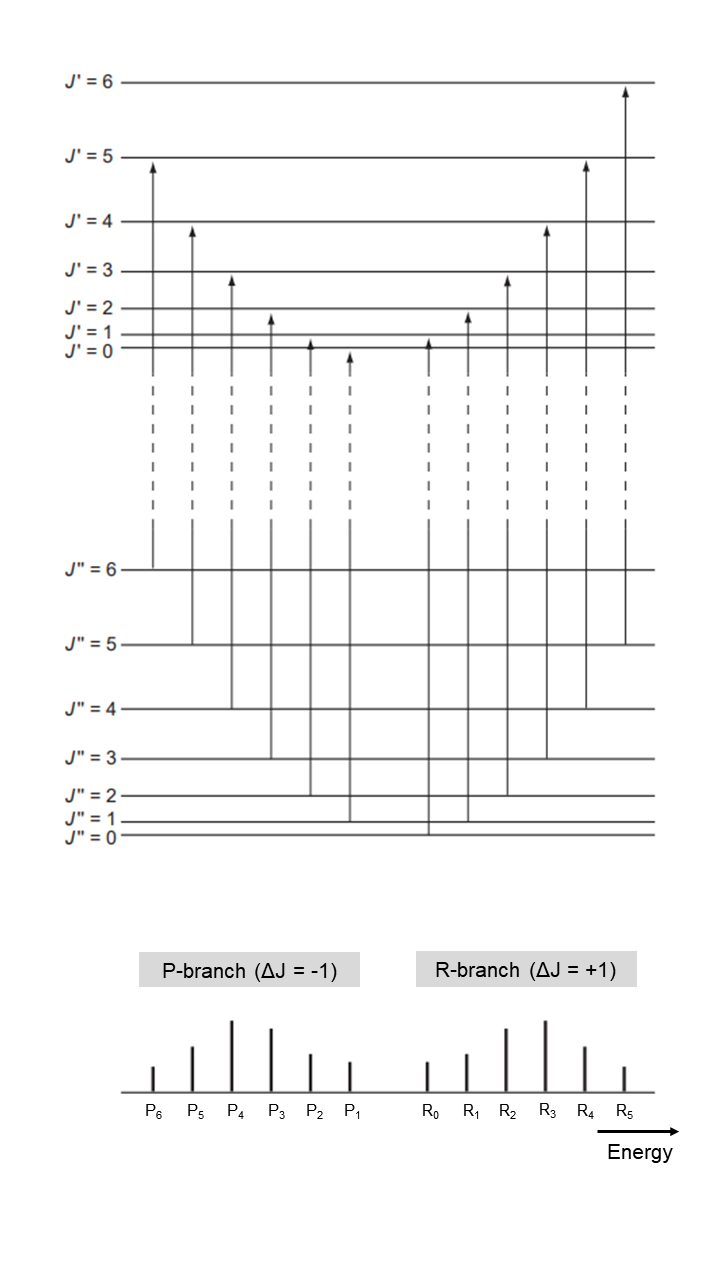
\includegraphics[width=7cm]{irspec}
	\centering
	\caption{A schematic IR spectrum}
	\label{fig:irspec}
\end{figure}
The vibrational state must possess an anisotropic dipole moment wrt. the normal coordinate. \Cref{irsymm} tells us whether a mode is IR-active.
\subsubsection{Raman spectroscopy}

Although complementary to IR spectroscopy, the theory of Raman spectroscopy is fundamentally different. 
An intense beam of laser at an appropriate, non-sweeping, monochromatic freqency is incident upon the sample, and the detector is placed at right angles to the incident beam to collect the scattered photons (note that no overall absorption of photons take place). The scattering can take place in three ways, we report $\Delta\nu$ and $\Delta J$ as ${\Delta\nu,\Delta J}$:
\begin{enumerate}
	\item \textbf{Rayleigh scattering}: Elastic scattering, no change in frequency of the photon, this corresponds to unchanged rot-vibrational level and hence ${0,0}$.
	\item \textbf{Stokes Raman scattering}: Inelastic scattering, reduced energy, corresponds to net excitation of rot-vibrational level, ${0,+2}$ or $+1,\pm2$.
	\item \textbf{Anti-Stokes Raman scattering}: Inelastic scattering, increased energy, corresponds to net relaxation, ${0,-2}$ or ${-1,\pm2}$.
\end{enumerate}
The $\Delta\nu=0$ corresponds to \emph{pure rotational Raman spectroscopy}, it uses low laser frequencies which do not have enough energy to excite the molecule to the next vibrational level, the $\Delta J=\pm2$ correspond to the Stokes and anti-Stokes branches, with the anti-Stokes branch having the same intensities as many rotational levels are thermally accessible at room temperature, so it does not matter whether the intial state is lower or higher. A schematic pure Rotational Raman spectrum is shown in \cref{fig:purerotspec} (the virtual levels are not shown)\footnote{As the branch lettering is $J_{\mathrm{upper}}-J_{\mathrm{lower}} $, both branches are technically $S$ in pure rotational Raman spectra.}:
\begin{figure}[H]
	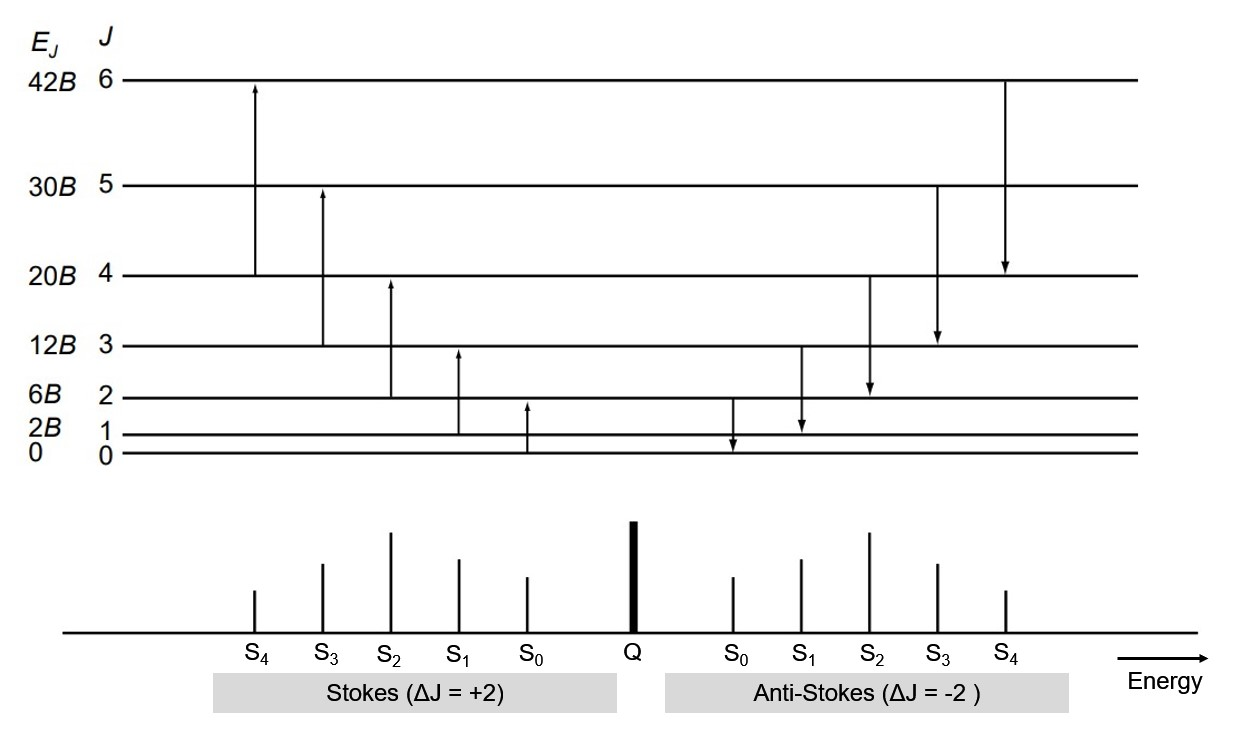
\includegraphics[width=12cm]{ramanspec}
	\centering
	\caption{A schematic pure rotational Raman spectrum}
	\label{fig:purerotspec}
\end{figure}
The $\Delta\nu=\pm1$ corresponds to \emph{vibrational Raman spectroscopy}, which uses high laser frequencies that are enough to excite the molecules vibrationally. The $\Delta\nu=+1$ is the Stokes branch and $\Delta\nu=-1$ is the anti-Stokes. The $\Delta J=\pm2$ should produce $O$- and $S$-branches as rotational fine structures but are too weak to observe in practice. A schematic vibrational Raman spectrum is shown in \cref{fig:vibraman}:
\begin{figure}[H]
	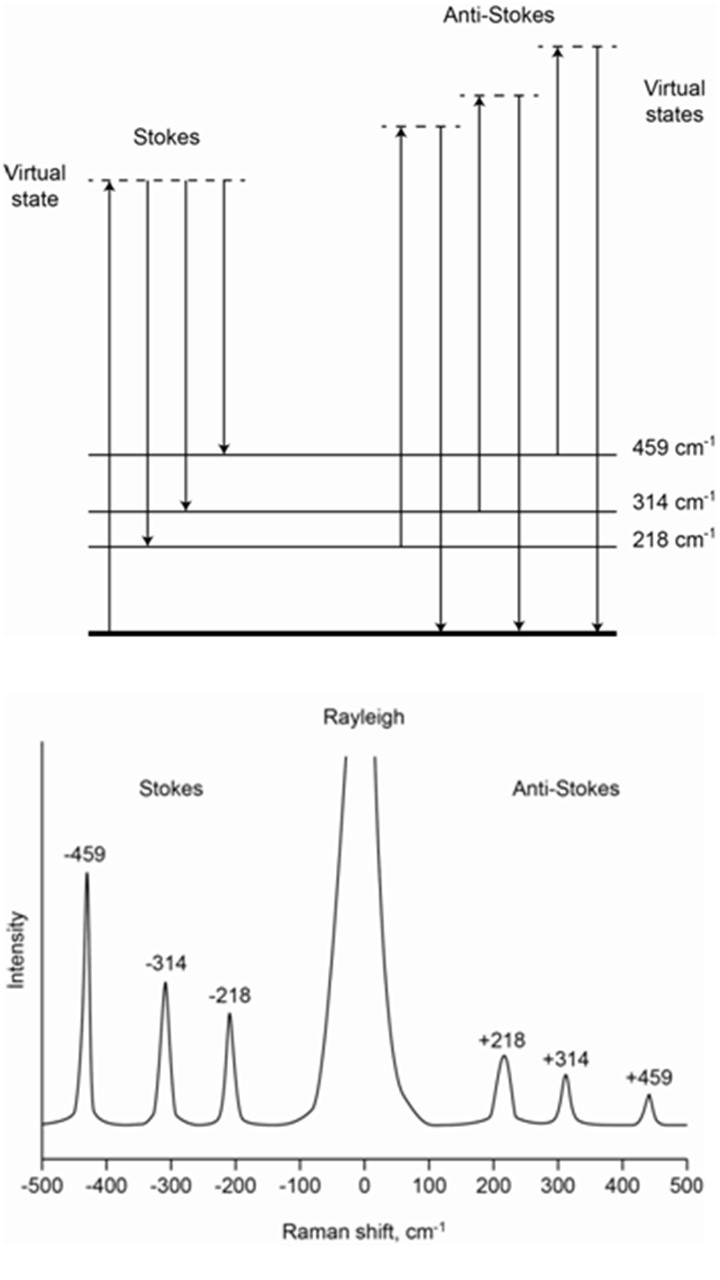
\includegraphics[width=8cm]{vibraman}
	\centering
	\caption{A schematic vibrational Raman spectrum}
	\label{fig:vibraman}
\end{figure}
Whether a vibrational mode is active in vibrational Raman spectroscopy is given by \Cref{irsymm} \hl{not written yet, update with thrm for Raman}.
\subsection{Transition frequencies}

\subsubsection{The vibrating rotor}
The vibrational spectral line spacings are derived from the Morse potential, with energy levels
\begin{equation}
	\ep_v=(v+\tfrac{1}{2} )\widetilde{\omega}-(v+\tfrac{1}{2} )^2\widetilde{\omega}x_e
\end{equation}
The depth of the well, $D_e$, can be found by finding $v_{\mathrm{max}} $, \ie setting $\diff{\ep_v}/{v}=0$:
\begin{equation}
\begin{aligned}
	D_e&=\ep_{\mathrm{max}}-\ep_{\mathrm{ZPE}}\\
&=\frac{\widetilde{\omega}}{4x_e}=\frac{\hbar\omega}{4x_e}
\end{aligned}
\end{equation}
The bond dissociation energy can be found by taking the difference of the well depth and ground state energy:
\begin{equation}
	\ep_B=\widetilde{D}_e-\ep_0=\widetilde{D}_e(1-x_e)^2
\end{equation}
The selection rule for the harmonic oscillator, $\Delta v=\pm 1$, proven in \cref{harmsele}, no longer hold true for the Morse oscillator, where we have $\Delta v=\pm1,\pm2\dots$. However usually only the $0\rightarrow1$ (fundamental), $0\rightarrow2$ (first overtone) are strong and, with the temperature-dependent\footnote{The other bands are not temperature dependent because they all only involve transitions from the ground state which is always thermally accessible.} $1\rightarrow2$ (hot band) and the $0\rightarrow3$ (second overtone) very weak.\par
The transtion frequencies are easy to calculate, some are listed here
\begin{center}
	\begin{tabular}{c|cccc}
	Transition & $0\rightarrow1$ & $0\rightarrow2$ & $0\rightarrow3$ & $1\rightarrow2$\\
	\hline
	$\Delta\ep$&$\widetilde{\omega}-2\widetilde{\omega}x_e $&$2\widetilde{\omega}-6\widetilde{\omega}x_e $&$3\widetilde{\omega}-12\widetilde{\omega}x_e $&$\widetilde{\omega}-4\widetilde{\omega}x_e $
	\end{tabular}
\end{center}
Because the vibrational wavefunction $\psi_n(x\equiv r-r_e)$ and the rotational 
wavefunction $Y^m_J(\theta,\phi)$ have different dependence, \ie degree of 
freedom. Therefore they are independent and we can write (we now adapt the notation in \Cref{vibindex})
\begin{equation}
\begin{aligned}
H\psi_{\mathrm{rot-vib}}&\equiv(H_{\mathrm{rot}}+H_{\mathrm{vib}})Y^m_J\psi_v\\
&=(E_J+E_v)Y^m_J\psi_v\\
&=\lf[BJ(J+1)+\hbar\omega\lf(v+\frac{1}{2}\rt)\rt]\psi_{\mathrm{rot-vib}}
\end{aligned}
\end{equation}
The convention is to write the energies in units of wavenumbers:
\begin{equation}
\widetilde{E}_{v,J}=\widetilde{B}J(J+1)+\widetilde{v}\lf(v+\frac{1}{2}\rt), 
\end{equation}
where 
\begin{equation}
\widetilde{B}=\frac{\hbar}{4\pi\widetilde{c}I},\ \widetilde{v}=\frac{1}{2\pi \widetilde{c}}\sqrt{\frac{k}{\mu}}.
\end{equation}
\begin{equation}
\begin{aligned}
&\Delta v=\pm1\ \text{(overtones allowed but weak)};\\
&\Delta J=\pm1.
\end{aligned}
\end{equation}
We have derived the vibrational spectral frequencies and the rotational frequencies as fine structures around the central vibrational freqencies. There's one problem we need to address, which is that the rotational constant $\widetilde{B}$ is not the same for each vibrational level because $\lgl r \rgl $ increases as vibrational states increases\footnote{This is evident if we examine the functional form of the Morse potential - the oscillator spends more time on the right than the left as the vibrational states are ascended.}. We need to account for that in our derivation for exact frequencies in the rotational fine structure below: 
\begin{equation}
\begin{aligned}
\widetilde{R}_{J''}&=\widetilde{E}_{v=1,J'=J''+1}-\widetilde{E}_{v=0,J''}\\
&=\lf(v+\frac{3}{2} \rt)\tilde{v}+\widetilde{B}_1(J''+1)(J''+2)-\lf(v+\frac{1}{2} \rt)\tilde{v}-\widetilde{B}_0J''(J''+1)\\
&=\tilde{v}_0+(\widetilde{B}_1-\widetilde{B}_0)J''^2+(3\widetilde{B}_1-\widetilde{B}_0)J''+2\widetilde{B}_1 ,\ J''=0,1,2,\cdots. 
\end{aligned}
\end{equation}
Likewise, the $P$-branch has 
\begin{equation}
\widetilde{P}_{J''}=\tilde{v}+(\widetilde{B}_1-\widetilde{B}_0)J''^2-(\widetilde{B}_1+\widetilde{B}_0)J'',\ J''=1,2,3,\cdots, 
\end{equation}
where $J''$ cannot be zero as this implies $J'$ starts at $-1$.\par
In the approximation that $\widetilde{B}_1=\widetilde{B}_0\equiv\widetilde{B}$, we arrive at 
\begin{equation}
\begin{aligned}
&\widetilde{R}_{J''}=\tilde{v}_0+2\widetilde{B}(J''+1)\\
&\widetilde{P}_{J''}=\tilde{v}_0-2\widetilde{B}J''.
\end{aligned}
\end{equation}
\begin{prt}[P and R branch peaks]
\begin{equation}
\begin{aligned}
&(\Delta J=+1)\ \widetilde{R}_{J}=\tilde{v}_0+2\widetilde{B}_1+(3\widetilde{B}_1-\widetilde{B}_0)J+(\widetilde{B}_1-\widetilde{B}_0)J^2 ,\ J=0,1,2,\cdots\\
&(\Delta J=-1)\ \widetilde{P}_{J}=\tilde{v}_0-(\widetilde{B}_1+\widetilde{B}_0)J+(\widetilde{B}_1-\widetilde{B}_0)J^2,\ J=1,2,3,\cdots
\end{aligned}
\end{equation}
\end{prt}
Now, the equilibrium bond length increases as we go up in $v$ with the Morse potential so 
$I$ goes up and $\widetilde{B}$ goes down, so the term $(\widetilde{B}_1-\widetilde{B}_0)J''^2$, although small, 
is always negative and increasingly so with increasing $J''$. 
This means the $P$ branch will be `streched' and the $R$ branch will be `compressed' more and more 
away from the central frequency. 
\subsubsection{Determination of rotational constants}
The general expression for any $J$-transition from $v=0$ to $v=1$ is 
\begin{equation}
\Delta\epsilon=\widetilde{v}_0+\widetilde{B}_1J'(J'+1)-\widetilde{B}_0J''(J''+1).
\end{equation}
Considering peaks originating from the same $J''$ (lower $J$), this gives rise to two peaks, one in the 
$P$ branch and one in the $R$ branch, both labelled with the same $J$ 
(conventionally labelled with lower $J$), and the difference is
\begin{equation}
\widetilde{R}_J-\widetilde{P}_J=2\widetilde{B}_1(2J+1).
\end{equation}
Similarly, for the same $J'$, we can find $\widetilde{B}_0$:
\begin{equation}
\widetilde{R}_{J-1}-\widetilde{P}_{J+1}=2\widetilde{B}_0(2J+1)
\end{equation}
\begin{prt}[Determination of rotational constants]
\begin{equation}
\begin{aligned}
&\widetilde{R}_J-\widetilde{P}_J=2\widetilde{B}_1(2J+1)\\
&\widetilde{R}_{J-1}-\widetilde{P}_{J+1}=2\widetilde{B}_0(2J+1)
\end{aligned}
\end{equation}
\end{prt}
Generally it is assumed that
\begin{equation}
\widetilde{B}_v=\widetilde{B}_e-\widetilde{\alpha}\lf(v+\frac{1}{2} \rt),
\end{equation}
where we need two $\widetilde{B}$'s to determine the equilibrium rotational constant of a hypothetical vibrationless molecule. This can then be used to determine the true equilibrium bond length. 
\subsubsection{Q-branch}
The selection rule $\Delta J=\pm1$ for IR spectroscopy holds true strictly for \emph{parallel vibrations} of linear molecules only, for molecules that have a perpendicular component of angular momentum, $\Delta J=0$ is possible\footnote{$J$ is \emph{defined} as the angular momentum in the direction of the principal axis, note this is the intrinsic axis instead of the laborartory $z$-axis which defines $m$.}. Examples include

\begin{itemize}
	\item Any non-linear molecule, as there are other axes of rotation other than the principal axis, the angular momentum about which $J$ is defined.
	\item Linear triatomic molecules, which have two degenerate bending modes, which create an oscillating dipole perpendicular to the principal axis, can combine to give rotational motions about the principal axis. This is the \textit{vibrational angular momentum}. 
	\item Diatomics with electronic orbital angular momentum, like NO, whose ground state term symbol is $^2\Pi$, this angular momentum is intrinsic in origin, rather than induced by vibration
\end{itemize}
Since all quantum mechanical angular momenta are quantised in the same way (in steps of $\hbar$), a photon can excite these angular momenta. This means that conservation of angular momentum is now possible without 
a change in $J$, 
\begin{prt}[Selection rules for perpendicular vibrations]
\begin{equation}
\begin{aligned}
&\Delta J=0,\ \pm1\\
&\Delta v=\pm1,\ \pm2,\ \cdots
\end{aligned}
\end{equation}
\end{prt}
The $Q$-branch consists of all transitions with the same $J$, and the frequencies are given by 
\begin{equation}
\begin{aligned}
\epsilon'-\epsilon''=&\lf[\lf(1+\frac{1}{2}\rt)\widetilde{\omega}-\lf(1+\frac{1}{2}\rt)^2\widetilde{\omega}x_e +\widetilde{B}_1J(J+1) \rt]-\\
&\lf[\lf(0+\frac{1}{2}\rt)\widetilde{\omega}-\lf(0+\frac{1}{2}\rt)^2\widetilde{\omega}x_e +\widetilde{B}_0J(J+1)\rt]\\
=&\widetilde{\omega}-2\widetilde{\omega}x_e+(\widetilde{B}_1-\widetilde{B}_0)J(J+1)\\
\equiv&\widetilde{\omega}_0+(\widetilde{B}_1-\widetilde{B}_0)J(J+1).
\end{aligned}
\end{equation}
\begin{prt}[$Q$-branch peaks]
$Q$-branch peaks occur at
\begin{equation}
\widetilde{\omega}_0+(\widetilde{B}_1-\widetilde{B}_0)J(J+1).
\end{equation}
\end{prt}
As $(\widetilde{B}_1-\widetilde{B}_0)$ is small, and \emph{positive} in this case as bending will result in smaller moment of inertia, this results in the spreading (towards higher wavenumbers) out of the Q-branch. This has effects on the $P$- and $R$-branches as well: now $R$ branch will be spread out away from the central freqency and $P$ will be compressed away from the central freqency, opposite of that in parallel strectches. All this is shown in \cref{fig:qbranch}
\begin{figure}[H]
	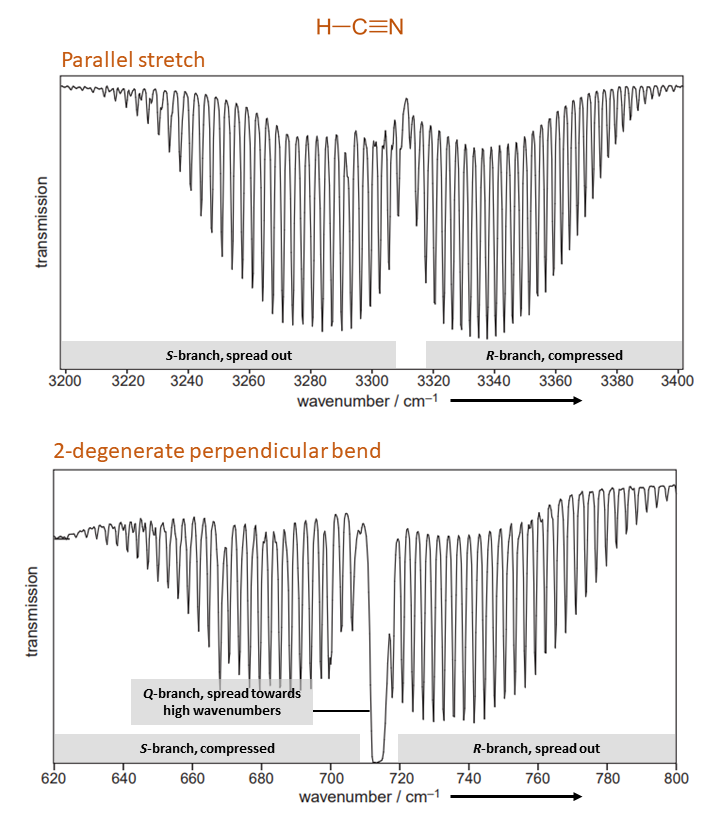
\includegraphics[width=12cm]{qbranch}
	\centering
	\caption{The IR spectrum of HCN, showing $Q$ branch in only one of the vibrational modes.}
	\label{fig:qbranch}
\end{figure}
The presence of $Q$-branch can be a diagnostic
\begin{prt}[Presence of $Q$-branch]
The absence of $Q$-branch in any of the vibrational modes proves that the molecule has to be linear.
\end{prt}
\subsection{Polyatomic molecules}
\label{polyvib}
\subsubsection{Normal coordinates}
\begin{thrm}[Normal coordinates]
\label{sym_of_vibfun}
In any molecular vibration mode $i$ it is always possible to define a normal coordinate $Q_i$ that can replace the scaled coordinate $q$ in the vibrational wavefunction.
\end{thrm}
\begin{proof}
	The problem with polyatmoic molecules is that they have $3N-5$ (linear) or $3N-6$ (non-linear) normal modes, therefore the same number of vibrational coordinates, $q_i$, and we can write the change in potential energy as
\begin{equation}
\begin{aligned}
	\dif V&=\frac{1}{2}\sum_{i=1}^{N_{\mathrm{vib}}}\sum_{j=1}^{N_{\mathrm{vib}}}\diffp{V}{q_i,q_j}q_iq_j+(\text{higher derivatives})\\
	&=\frac{1}{2}\sum_{i=1}^{N_{\mathrm{vib}}}\sum_{j=1}^{N_{\mathrm{vib}}}f_{ij}q_iq_j+\dots
\end{aligned}
\end{equation}
Unfortunately, the cross-terms makes the \sch intractable. A theorem from classical mechanics can transform the cross terms into \emph{normal coordinates}:
\begin{equation}
	\dif V\approx\frac{1}{2}\sum_{j=1}^{N_{\mathrm{vib}}}F_jQ_j^2
\end{equation}
\end{proof}
\begin{prt}[Symmetry of normal coordinates]
The normal coordinate $Q_i$ has the same symmetry as the normal mode.
\end{prt}
\begin{proof}
	The normal coordinate $Q_i$ \emph{defines} the normal mode as the linear combination of vibrational coordinates that make up the normal mode. Therefore \emph{must} transform as the symmetry species of the normal mode. This pointing out the chicken-and-egg situation rather than a proof.
\end{proof}
\subsubsection{Symmetry of vibrational wavefunctions}
As the transition probability involves evaluating integrals of the form $\lgl \psi_i |\bvec{\mu}|\psi_j  \rgl $, we need to work out the symmetry species spanned by the vibrational wavefunctions. 
\begin{thrm}[Symmetry of vibrational wavefunctions]
For harmonic oscillators, odd state vibrational wavefunctions always transform as the totally symmetric IR.\par
Even state vibrational wavefunctions always transform as the IR of the normal mode.\par
For degenerate normal modes, the first excited state transforms as the normal mode, but higher excited states are more complex \hl{what?}
\end{thrm}
\begin{proof}
	As the unnormalised ground state is
	\begin{equation}
		\psi_0=e^{-\frac{1}{2}Q_i^2}
	\end{equation}
	For a non-degenerate irrep, this must return characters as 1's, \ie the totally symmetric IR.\par
	The first excited state is
	\begin{equation}
		\psi_1=Q_ie^{-\frac{1}{2}Q_i^2},
	\end{equation}
	we know the exponential bit transforms as the tot. sym. IR, and that $Q_i$ transforms as the normal mode (\Cref{sym_of_vibfun}), therefore $\psi_1$ transforms as the symmetry species of the normal mode. \par
	The form of the Hermite polynomials \hl{is this true? specific only to Hermite?} dictates that even-numbered functions contains only even exponents and constants, and that odd-numbered functions contains only odd exponents and no constants, \ie factorisable to $[Q_i(\text{tot. sym. function})]$, which means they all transform as the normal mode. 
\end{proof}
\subsubsection{Symmetry selection rules for infrared}
For transition between energy levels of a single normal mode, we assume we start at the ground state, we need to know whether the integral
\begin{equation}
R_{v_i,v_i'}=\lgl\psi_{v_i'}|\mu|\psi_{v_i} \rgl
\end{equation}
is non-zero, where $\mu$ transforms like the principle Cartesian axes:
\begin{defi}[Dipole moment operator]
As the dipole moment $\bvec{\mu}$ is only dependent on the normal coordinate $\bvec{Q_i}$, we can write
\begin{equation}
\bvec{\mu}=\bvec{\mu}_0+\lf(\diff{\bvec{\mu}}{Q_i}\rt)_{Q_i=0} Q_i+\frac{1}{2}\lf(\diff[2]{\bvec{\mu}}{Q_i} \rt)_{Q_i=0}Q_i^2+\dots
\end{equation}
If we make the approximation that the partial charges are constant \ie dipole moment varies linearly with normal coordinate, with the first term vanished by orthonormality, we are left with the definition of the dipole moment:
\begin{equation}
\bvec{\mu}\equiv \lf(\diff{\bvec{\mu}}{x}\rt)_0 Q_i
\end{equation}
\end{defi}
Invoking theorem \hl{which one}, we arrive at the result
\begin{thrm}[Transition rules]
\label{irsymm}
For a fundamental transition (transitions from the ground state energy of a normal mode to an excited state of the same mode) to be allowed in infrared, the IR of the normal mode has to be the same as that of x, y or z.
\end{thrm}
However symmetry allowed transitions can still have their integrals evaluated to zero by functional forms determined not by symmetry. For example, the selection rule for the harmonic oscillator is $\nu=\pm 1$, this is derived from the ladder operators:\par
As stated above, we can always write the normal coordinate as 
\begin{equation}
Q_i=\lf(\frac{\hbar}{2\mu\omega} \rt)^{1/2}(a_-+a_+)
\end{equation}
where the ladder operators also have their scaled coordinate replaced by the normal coordinate. It is now easy to write
\begin{equation}
\label{harmsele}
\begin{aligned}
\lgl v_i|\bvec{\mu}|v_j\rgl&\propto \lgl v_i|(a_-+a_+)|v_j \rgl\\
&=\delta_{i,j-1}+\delta_{i,j+1}
\end{aligned}
\end{equation}
and it is apparent that only when $j=i\pm 1$, the matrix element is nonzero. 
\subsection{Electronic spectroscopy}

\subsubsection{The Franck-Condon principle}
The Einstein B coefficient for induced absorption or emission\footnote{The A coefficient is for spontaneous emission.} is given as 
\begin{equation}
\label{einsteincoeff}
	B_{mn}=\frac{1}{3\ep_0\hbar^2}|\lgl \psi_m |\uvec{\mu}|\psi_n  \rgl|^2
\end{equation}
Under the Born-Oppenheimer approximation, ignoring the rotational changes, as they are too fine to be resolved, we can write
\begin{equation}
	\psi_i=\psi_{i,E}\psi_{i,V},\ \uvec{\mu}=\uvec{\mu}_E+\uvec{\mu}_V
\end{equation}
The transition dipole moment is now
\begin{equation}
\begin{aligned}
	&|\lgl \psi'' |\uvec{\mu}|\psi'  \rgl|^2\\
	=&|\lgl \psi''_E\psi''_V|\uvec{\mu}_E+\uvec{\mu}_V |\psi_E'\psi_V'  \rgl |^2\\
	=&|\lgl \psi''_E\psi''_V|\uvec{\mu}_E|\psi_E'\psi_V'  \rgl+\lgl \psi''_E\psi''_V|\uvec{\mu}_V|\psi_E'\psi_V'  \rgl |^2\\
	=&|\lgl \psi''_E|\uvec{\mu}_E|\psi_E'  \rgl \lgl \psi''_V | \psi_V' \rgl+ \lgl \psi''_E | \psi_E' \rgl \lgl \psi''_V|\uvec{\mu}_V|\psi_V'  \rgl |^2\\
	=&|\lgl \psi''_E|\uvec{\mu}_E|\psi_E'  \rgl|^2 |\lgl \psi''_V | \psi_V' \rgl|^2
\end{aligned}
\end{equation}
The electronic wavefunctions are orthonormal, but not the vibrational states \emph{belonging to different electronic states} as they are on different Morse potentials and are solutions to different Schro\"dinger equations.\par
The first bit is the electronic transition dipole, and group theory can tell us whether that vanishes. The second part is known as the \emph{Franck-Condon factor}, which tells us the extent of overlap between two vibrational wavefunctions. The \emph{Franck-Condon principle} is the assumption that there's no change in bond length before and after the electronic transition \ie the overlap F-C factor can tell us the probability of transition.
\begin{thrm}[The Franck-Codon principle]
Because the nuclei are much more massive than electrons, an \emph{electronic} transition takes place while the nuclei in a molecule are effectively stationary. The transition probability between two vibrational states in two electronic states is given by $|\lgl \psi''_V | \psi_V' \rgl|^2$.
\end{thrm}
This will give progressions that start from the lower vibrational states $v''=0,1,2,\dots$, which each successive progression at lower wavenumbers and lower intensities as the states become less populated.\par
The transition energies can be represented as follows
\begin{equation}
\begin{aligned}
	\widetilde{v}'-\widetilde{v}''&=(\ep_0'-\ep_0'')+\{[(v'+\tfrac{1}{2})\widetilde{\omega}'_e-\widetilde{\omega}'_ex_e'(v'+\tfrac{1}{2} )^2]-[(v''+\tfrac{1}{2})\widetilde{\omega}''_e-\widetilde{\omega}''_ex_e''(v''+\tfrac{1}{2} )^2]\}\\
	&\equiv T_e+\Delta \widetilde{E}_v 
\end{aligned}
\end{equation}
This allows us to compute parameters such as the equilibrium bond length and the dissociation energy of an excited electronic mode.

\chapter{Approximation methods}
The Hamiltonian for a general neutral atom with nuclear charge $Ze$ is
\begin{equation}
\label{genham}
H=\underbrace{\sum^Z_{j=1}\lf[-\frac{\hbar^2}{2m}\onabla^2_j-\lf(\frac{1}{4\pi\epsilon_0}\frac{Ze^2}{r_j} \rt) \rt]}_{\text{kinetic energy}+\text{nuclear attraction}}+\underbrace{\vphantom{\sum^Z_{j=1}\lf[-\frac{\hbar^2}{2m}\onabla^2_j-\lf(\frac{1}{4\pi\epsilon_0}\frac{Ze^2}{r_j} \rt) \rt]}\frac{1}{2}\lf(\frac{1}{4\pi\epsilon_0} \rt)\sum_j^Z\sum^Z_{k\neq j}\frac{e^2}{|\bvec{r}_j-\bvec{r}_k|}}_{\text{interelectronic repulsion}}.
\end{equation}
The factor of $1/2$ merely corrects for the fact that the double summation counts 
over each pair twice. We then wish to solve for
\begin{equation}
H\psi(\bvec{r}_1,\bvec{r}_2,\cdots,\bvec{r}_Z)=E\psi(\bvec{r}_1,\bvec{r}_2,\cdots,\bvec{r}_Z).
\end{equation}
And the only acceptable solutions according to the symmetrisation requirement is 
when, coupled with the spin, the complete wavefunction is antisymmetric wrt 
exchange of electrons. \\
This equation cannot be solved exactly and we must resort to approximation methods 
which will be discussed in this chapter. 
\section{The variational method}
\subsection{Theory}
Consider now the ground state of an arbitrary system. The ground state \sch states
\begin{equation}
H|\psi_0\rgl=E_0|\psi_0\rgl.
\end{equation}
Right-multiplying by $\lgl\psi_0|$ we have
\begin{equation}
E_0=\frac{\lgl \psi_0|H|\psi_0\rgl}{\lgl \psi_0|\psi_0\rgl}
\end{equation}
We introduce the theorem
\begin{thrm}[The variational principle]
For \textit{any other} arbitrary function $\phi$ with the same arguments (provided 
that the integral exists of course), the corresponding energy
\begin{equation}
\label{energyphi}
E_{\phi}=\frac{\lgl \phi|H|\phi\rgl}{\lgl \phi|\phi\rgl}
\end{equation}
must have that
\begin{equation}
E_{\phi}\geq E_0,
\end{equation}
where the equality holds only for $\phi=\psi_0$.
\end{thrm}
\begin{proof}
Because the set of eigenfunctions of $H$ is complete, we can express \textit{any} 
function $\phi$ as 
\begin{equation}
|\phi\rgl=\sum^{\inf}_{n=0}  c_n|\psi_n\rgl.
\end{equation}
Where, from the orthonormality of $\psi_n$'s,
\begin{equation}
c_n=\lgl \psi_n|\phi\rgl.
\end{equation}
So \Cref{energyphi} now reads
\begin{equation}
E_{\phi}=\frac{\lgl \phi|H|\phi\rgl}{\lgl \phi|\phi\rgl}=\frac{c_n^*c_n\lgl \sum\psi_n|H|\sum \psi_n\rgl}{c_n^*c_n\lgl \sum\psi_n|\sum \psi_n\rgl}=\frac{\sum |c_n|^2E_n}{\sum |c_n|^2}.
\end{equation}
Subtracting $E_0$ from both sides, we have
\begin{equation}
E_{\phi}-E_0=\frac{\sum |c_n|^2(E_n-E_0)}{\sum |c_n|^2},
\end{equation}
which \textit{must} be non-negative as $E_n$ is by definition greater than $E_0$, 
and all $|c_n|^2$ are non-negative as well. And we obeserve that the equality 
holds necessarily when $\phi=\psi_0$ since all non-zero $c_n$'s must be $0$, but 
at $n=0$, $E_n=E_0$ also, so the entire summation in the numerator vanishes for 
all $n$. 
\end{proof}
The variational principle says that we can get an upper bound to $E_0$ by using 
any trial function as we wish, with closer approxmation if $\phi$ is functionally 
more similar to $\psi_0$. In general, we will choose a trial function that 
depends on some arbitrary \textit{variational parameters}, $\alpha,\beta,\gamma,\cdots$. The energy then will also depend upon these parameters, \ie
\begin{equation}
E_{\phi}(\alpha,\beta,\gamma,\cdots)\geq E_0.
\end{equation}
Now we can minimise $E_{\phi}$ wrt each of the parameters, so the best possible 
ground-state energy of a specific trial wavefunction can be found.
\subsection{Examples}
\textbf{Hydrogen ground state}\\
As an example, we try to approximate the hydrogen ground state wavefunction. We just need to know the Hamiltonian:
\begin{equation}
H=\frac{\hbar^2}{2m}\diff{}{r}\lf(r^2\diffp{}{r} \rt)-\frac{e^2}{4\pi\epsilon_0r}.
\end{equation}
Say we guess that the wavefunction is a Gaussian (and we know from empirical 
evidence that it will not depend on $\theta$ and $\phi$):
\begin{equation}
\phi(r)=e^{-\alpha r^2}.
\end{equation}
Let's now calculate $E_{\phi}$.
\begin{equation}
\lgl \phi|H|\phi\rgl=4\pi\intinfp\phi^*(r)H\phi(r)r^2\dif r=\frac{3\hbar^2\pi^{3/2}}{4\sqrt{2}m\alpha^{1/2}}-\frac{e^2}{4\epsilon\alpha},
\end{equation}
where we have used the standard integrals in \Cref{integrals}. Similarly, 
\begin{equation}
\lgl \phi|\phi\rgl=4\pi\intinfp\phi^*\phi r^2\dif r=\lf(\frac{\pi}{2\alpha} \rt)^{3/2}
\end{equation}
where we note that in general, these trial functions are, of course, not 
normalised, but nowhere in the derivation of the variational principal required 
that the wavefunctions, trial or actual, be normalised. \\
We can therefore compute the trial energy
\begin{equation}
E(\alpha)=\frac{3\hbar^2\alpha}{2m}-\frac{e^2\alpha^{1/2}}{\sqrt{2}\epsilon_0\pi^{3/2}}.
\end{equation}
Setting the first derivative to zero we obtain
\begin{equation}
\alpha_{\text{min}}=\frac{m^2e^4}{18\pi^3\epsilon_0^2\hbar^4},
\end{equation}
so
\begin{equation}
E_{\text{min}}=-\frac{4}{3\pi}\lf(\frac{me^4}{16\pi^2\epsilon_0^2\hbar^2} \rt)\approx-0.424\lf(\frac{me^4}{16\pi^2\epsilon_0^2\hbar^2} \rt),
\end{equation}
where the exact value is
\begin{equation}
E_0=-0.500\lf(\frac{me^4}{16\pi^2\epsilon_0^2\hbar^2} \rt).
\end{equation}
Pretty good approximation despite the wrong choice of trial function. And sure 
enough, by using the trial function of 
\begin{equation}
\phi=e^{-\alpha r}
\end{equation}
we can get the exact ground state energy and wavefunction. \\
\ \\
\textbf{Helium ground state}\\
The previous example was based on a system we do know hwo to solved exactly, and 
now we apply it to one that we don't: the helium atom, with the Hamiltonian
\begin{equation}
\begin{aligned}
H&=-\frac{\hbar^2}{2m}(\onabla^2_1+\onabla_2^2)-\frac{e^2}{2\pi\epsilon}\lf(\frac{1}{r_1}+\frac{1}{r_2} \rt)+\frac{e^2}{4\pi\epsilon_0}\frac{1}{r_{12}}\\
&=H_{1}+H_2+\frac{e^2}{4\pi\epsilon_0}\frac{1}{r_{12}},
\end{aligned}
\end{equation}
where $H_i$'s are the Hamiltonian for a single electron atom with $Z=2$, and 
they satisfy the equation
\begin{equation}
H_i\psi(r_i,\theta_i,\phi_i)=E_i\psi(r_i,\theta_i,\phi_i).
\end{equation}
We choose our trial function by ignoring the interelectronic repulsion term, \ie
\begin{equation}
\phi_0(\bvec{r}_1,\bvec{r}_2)=\psi_{1s}(\bvec{r}_1)\psi_{1s}(\bvec{r}_2),
\end{equation}
where $\psi_{1s}$ is the $Z=2$ ground state hydrogenlike wavefunction:
\begin{equation}
\psi_{1s}(\bvec{r}_i)=\lf(\frac{Z^3}{\pi a^3} \rt)^{1/2}e^{-Zr_i/a},\ i=1,2.
\end{equation}
So our trial function is 
\begin{equation}
\phi(\bvec{r}_1,\bvec{r}_2)=\frac{Z^3}{a^3\pi}e^{-Z(r_1+r_2)/a}.
\end{equation}
As the trial function is normalised this time, we only have to evaluate the 
numerator:
\begin{equation}
E(Z)=\iint \phi_0^*(\bvec{r}_1,\bvec{r}_2)H\phi_0(\bvec{r}_1,\bvec{r}_2)\dif \bvec{r}_1\dif\bvec{r}_2.
\end{equation}
This integral can seem daunting but we can greatly simplify it by realising $\psi$ 
is an eigenfunction of the hydrogenlike Hamiltonian:
\begin{equation}
H\psi=-\frac{Z^2\hbar^2}{2ma^2}\psi.
\end{equation}
We now re-write the Helium Hamiltonian in terms of hydrogenlike Hamiltonians, 
keeping in mind that $Z$ is not necessarily $2$ now as it is a variational parameter:
\begin{equation}
\begin{aligned}
H&=-\frac{\hbar^2}{2m}(\onabla^2_1+\onabla_2^2)-\frac{e^2}{2\pi\epsilon}\lf(\frac{1}{r_1}+\frac{1}{r_2} \rt)+\frac{e^2}{4\pi\epsilon_0}\frac{1}{r_{12}}\\
&=-\frac{\hbar^2}{2m}\onabla_1^2-\frac{Ze^2}{4\pi\epsilon_0r_1}-\frac{\hbar^2}{2m}\onabla_2^2-\frac{Ze^2}{4\pi\epsilon_0r_2}+\frac{(Z-2)e^2}{4\pi\epsilon_0r_1}+\frac{(Z-2)e^2}{4\pi\epsilon_0r_2}+\frac{e^2}{4\pi\epsilon_0r_{12}}\\
&=H_{Z1}+H_{Z2}+\frac{(Z-2)e^2}{4\pi\epsilon_0r_1}+\frac{(Z-2)e^2}{4\pi\epsilon_0r_2}+\frac{e^2}{4\pi\epsilon_0r_{12}}.
\end{aligned}
\end{equation}
So
\begin{equation}
\begin{aligned}
E(Z)=&\iint\phi\lf[-\frac{Z^2\hbar^2}{2ma^2}-\frac{Z^2\hbar^2}{2ma^2}+\frac{(Z-2)e^2}{4\pi\epsilon_0r_1}+\frac{(Z-2)e^2}{4\pi\epsilon_0r_2}+\frac{e^2}{4\pi\epsilon_0r_{12}} \rt]\phi\dif \bvec{r}_1\dif \bvec{r}_2\\
=&\frac{Z^6}{a^6\pi^2}16\pi^2\iint\lf[-\frac{Z^2\hbar^2}{ma^2}+\frac{(Z-2)e^2}{4\pi\epsilon_0r_1}+\frac{(Z-2)e^2}{4\pi\epsilon_0r_2} \rt]e^{-2Z(r_1+r_2)/a}r_1^2r_2^2\dif r_1\dif r_2\\
&+\frac{Z^6}{a^6\pi^2}\iint \frac{e^2}{4\pi\epsilon_0r_{12}}e^{-2Z(r_1+r_2)/a}\dif \bvec{r}_1\dif \bvec{r}_2 \\
=&\frac{16Z^6}{a^6}\iint\lf[-\frac{Z^2e^2}{4\pi\epsilon_0 a}+\frac{(Z-2)e^2}{4\pi\epsilon_0r_1}+\frac{(Z-2)e^2}{4\pi\epsilon_0r_2} \rt]e^{-2Z(r_1+r_2)/a}r_1^2r_2^2\dif r_1\dif r_2\\
&+\frac{Z^6}{a^6\pi^2}\iint \frac{e^2}{4\pi\epsilon_0r_{12}}e^{-2Z(r_1+r_2)/a}\dif \bvec{r}_1\dif \bvec{r}_2
\end{aligned}
\end{equation}
We have isolated the integral involving $r_{12}$ because they are implicitly 
dependent on $\theta$. There are four integrals to solve, for the first three we 
use the standard integral \Cref{integral1}:
\begin{equation}
\begin{aligned}
&\frac{16Z^6}{a^6}\iint-\frac{Z^2}{4\pi\epsilon_0 a}e^{-2Z(r_1+r_2)}r_1^2r_2^2\dif r_1\dif r_2\\
=&-\frac{4Z^8e^2}{\pi\epsilon_0 a^7}\lf(\int e^{-2Zr/a}r^2\dif r\rt)^2\\
=&-\frac{4Z^8e^2}{\pi\epsilon_0 a^7}\lf(\frac{a^3}{4Z^3}\rt)^2\\
=&-\frac{Z^2e^2}{4\pi\epsilon_0a}\\
=&-Z^2\lf(\frac{me^4}{16\pi^2\epsilon_0^2\hbar^2} \rt)=-Z^2\ \text{Hartree},
\end{aligned}
\end{equation}
and the second and third are the same integral:
\begin{equation}
\begin{aligned}
&\frac{16Z^6(Z-2)e^2}{4\pi\epsilon_0a^6}\iint r_1r_2^2e^{-2Z(r_1+r_2)/a}\dif r_1\dif r_2\\
=&\frac{16Z^6(Z-2)e^2}{4\pi\epsilon_0a^6}\frac{a^5}{16Z^5}\\
=&Z(Z-2)\ \text{Ha}.
\end{aligned}
\end{equation}
The last integral is trickier, we first need to choose the $z$-axis to be one of 
the vectors, say $\bvec{r}_1$, so we can use our usual spherical coordinates: 
\begin{equation}
r_{12}=(r_1^2+r_2^2-2r_1r_2\cos\theta)^{1/2}.
\end{equation}
The integral becomes
\begin{equation}
\begin{aligned}
&\frac{Z^6e^2}{4\pi^3\epsilon_0a^6}\iint\frac{1}{(r_1^2+r_2^2-2r_1r_2\cos\theta)^{1/2}}e^{-2Z(r_1+r_2)/a}\dif\bvec{r}_1\dif\bvec{r}_2\\
=&\frac{Z^6e^2}{4\pi^3\epsilon_0a^6}4\pi^2\int^{\pi}_0\sin\theta_2\dif\theta_2\intinfp\intinfp\int^{\pi}_0e^{-2Z(r_1+r_2)/a}r_1^2r_2^2\frac{\sin\theta_1\dif\theta_1\dif r_1\dif r_2}{(r_1^2+r_2^2-2r_1r_2\cos\theta_1)^{1/2}}\\
=&\frac{2Z^6e^2}{\pi\epsilon_0a^6}\intinfp\intinfp e^{-2Z(r_1+r_2)/a}r_1r_2(r_1^2+r_2^2-2r_1r_2\cos\theta_1)^{1/2}\Big|^\pi_0\dif r_1\dif r_2\\
=&\frac{2Z^6e^2}{\pi\epsilon_0a^6}\intinfp\intinfp e^{-2Z(r_1+r_2)/a}r_1r_2\lf[(r_1^2+r_2^2+2r_1r_2)^{1/2}-(r_1^2+r_2^2-2r_1r_2)^{1/2} \rt]\dif r_1\dif r_2.
\end{aligned}
\end{equation}
Now, the terms in the square brackets must be positive as we are computing 
energy. When $r_2<r_1$ we have the terms equal to $2r_2$, and when $r_2>r_1$ 
they are equal to $2r_1$. Making $r_1$ run from $0$ to infinity and splitting 
the integral over $r_2$ into two parts, the integral is 
\begin{equation}
\label{5z8}
\begin{aligned}
&\frac{2Z^6e^2}{\pi\epsilon_0a^6}\intinfp r_1e^{-2Zr_1/a}\dif r_1\lf(2\int_0^{r_1}r_2^2e^{-2Zr_2/a}\dif r_2+2r_1\int_{r_1}^{\inf}r_2e^{-2Zr_2/a}\dif r_2 \rt)\\
=&\frac{4Z^6e^2}{\pi\epsilon_0a^6}\intinfp r_1e^{-\alpha r_1}\lf[\frac{2}{\alpha^3}-\lf(\frac{r_1}{\alpha^2}+\frac{2}{\alpha^3} \rt)e^{-\alpha r_1} \rt]\dif r_1\\
=&\frac{4Z^6e^2}{\pi\epsilon_0a^6}\lf(\frac{2}{\alpha^5}-\frac{1}{4\alpha^5}-\frac{1}{2\alpha^5} \rt)\\
=&\frac{5Z}{8}\ \text{Ha}.
\end{aligned}
\end{equation}
Finally we can assemble the entire integral:
\begin{equation}
E(Z)=Z^2-\frac{27}{8}Z
\end{equation}
in Hartrees, minimising we have
\begin{equation}
Z_{\text{min}}=\frac{27}{16}\ \imp\ E_{\text{min}}\approx-2.8477.
\end{equation}
The experimental value is $-2.9033$, we have reached a pretty good approximation 
even when we have disregarded interelectronic repulsion completely. The 
variational principal in a way compensates that by returning us a $Z$ less 
than $2$, which can be understood as an \textbf{effective nuclear charge}.
\subsection{Secular determinants}
A trial function with more than one parameter can return very good results, as 
to be expected since the ground state wavefunction can be expressed as an infinite 
series of any functions, the more terms we include, the better we can approximate. 
We use a trial funciton of the form
\begin{equation}
\phi=\sum^N_{n=1}c_nf_n, 
\end{equation}
where $c_n$ are variational parameters and $f_n$ are arbitrarily chosen functions. 
We restrict ourselves to two terms, and $c_n$ and $f_n$ can be complex
\begin{equation}
\phi=c_1f_1+c_2f_2.
\end{equation}
To get $E_{\phi}$, we compute
\begin{equation}
\begin{aligned}
\lgl \phi|H\phi\rgl=&\lgl(c_1f_1+c_2f_2) |H(c_1f_1+c_2f_2) \rgl\\
=&|c_1|^2H_{11}+c_1^*c_2H_{12}+c_1c_2^*H_{21}+|c_2|^2H_{22},
\end{aligned}
\end{equation}
where 
\begin{equation}
H_{ij}=\lgl f_i|Hf_j\rgl.
\end{equation}
Similarly, 
\begin{equation}
\begin{aligned}
\lgl \phi|\phi\rgl=|c_1|^2S_{11}+c_1^*c_2S_{12}+c_1c_2^*S_{21}+|c_2|^2S_{22}.
\end{aligned}
\end{equation}
where 
\begin{equation}
S_{ij}=\lgl f_i|f_j\rgl.
\end{equation}
So we can write (to facilitate implicit differentiation)
\begin{equation}
|c_1|^2H_{11}+c_1^*c_2H_{12}+c_1c_2^*H_{21}+|c_2|^2H_{22}=E_{\phi}(|c_1|^2S_{11}+c_1^*c_2S_{12}+c_1c_2^*S_{21}+|c_2|^2S_{22}).
\end{equation}
We now minimise $E(c_1,c_2)$. However, we want the final expression to be in terms 
of $c_1$ and $c_2$, not their conjugates, purely for the sake of brevity, so 
we instead minimise $c_1^*$ and $c_2^*$:
\begin{equation}
\diffp{E}{c_1^*}=0\ \imp\ c_1(H_{11}-E{\phi}S_{11})+c_2(H_{12}-E_{\phi}S_{12})=0,
\end{equation}
and minimising $c_2^*$ we have
\begin{equation}
c_1(H_{21}-E_{\phi}S_{21})+c_2(H_{22}-E_{\phi}S_{22})=0.
\end{equation}
where we need the property, \textit{ad hoc}, that 
\begin{prt}[Complex differentiation]
\begin{equation}
\diffp fz=\frac{1}{2}\lf(\diffp fx-i\diffp fy\rt),\ \diffp{f}{z^*}=\frac{1}{2}\lf(\diffp fx+i\diffp fy\rt).
\end{equation}
\end{prt}
\begin{proof}
This is a heuristic proof and is not rigourous. See Cauchy-Riemann equation for 
theoretical foundation. Let
\begin{equation}
z\equiv x+iy,\ \imp\ z^*=x-iy, 
\end{equation}
so
\begin{equation}
x=\frac{1}{2}(z+z^*),\ y=-\frac{1}{2}i(z-z^*).
\end{equation}
So
\begin{equation}
\diffp fz=\diffp fx\diffp xz+\diffp fy\diffp yz=\frac{1}{2}\lf(\diffp fx-i\diffp fy\rt),
\end{equation}
and so on. 
\end{proof}
Anyway, casting the above equations in matrix form, we have
\begin{equation}
\begin{pmatrix}
H_{11}-E_{\phi}S_{11}&H_{12}-E_{\phi}S_{12}\\
H_{21}-E_{\phi}S_{21}&H_{22}-E_{\phi}S_{22}
\end{pmatrix}
\begin{pmatrix}
c_1\\
c_2
\end{pmatrix}=0,
\end{equation}
which means there will only be non-trivial solutions for $c_1$ and $c_2$ when 
the determinant
\begin{equation}
\begin{vmatrix}
H_{11}-E_{\phi}S_{11}&H_{12}-E_{\phi}S_{12}\\
H_{21}-E_{\phi}S_{21}&H_{22}-E_{\phi}S_{22}
\end{vmatrix}=0. 
\end{equation}
Determinants like this are called \textbf{secular determinants}. 
Expanding and solving them will give us a quadratic equation in $E_{\phi}$ without 
explicitly computing $c_n$. We take the smaller of the two solutions as the upper 
bound estimate. Once we have determined $E_{\phi}$ we can invert the matrix 
equation to find the $c_n$'s and subsequently normalise the approximate solution. 
This can be trivially generalised to trial functions of $N$ terms. \\
Just as an aside, the $f_n$'s themselves can include variational parameters to 
obtain even better approximations, but however we can't use secular determinants 
in that case and numerical computations are required. 
\subsection{The H{\" u}ckel approximations}
\label{huckel}
To compute the secular determinant more quickly, the H{\" u}ckel approximations can be used. The approximations are
\begin{enumerate}
\item The overlap integral $S_{ij}=0$ for $i\neq j$
\item The Hamiltonian matrix element is nonzero only for neighouring atoms.
\end{enumerate}
A number of simplified notations are adopted:
\begin{enumerate}
\item $H_{ii}\equiv\alpha_{ii}\equiv\alpha$
\item $H_{ij}\equiv\beta_{ij}=\beta_{ji}$
\end{enumerate}
The method proceeds as follows
\begin{enumerate}
	\item Find out the point group the molecule belongs to
	\item Identify unique sets of orbitals that are interconverted, and discard those belonging to the same symmetry species, \ie they are never interconverted
	\item Reduce the representation
	\item Set up symmetry orbitals for all sets of orbitals
	\item Solve the secular equation for symmetry orbitals belonging to the same symmetry to obtain energyies and coefficients
\end{enumerate}
This is a long list, and it best illustrated by examples
\subsubsection{Example 1}
\begin{figure}[H]
	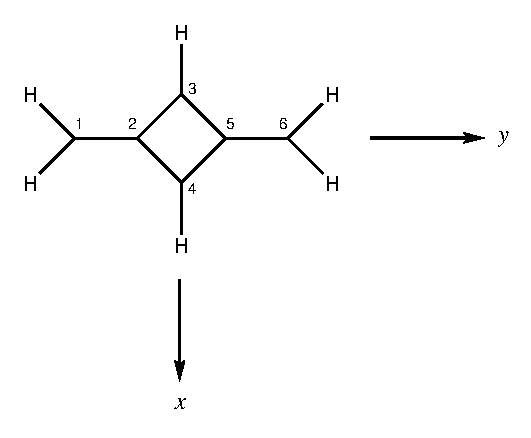
\includegraphics[width=6cm]{huckel1}
	\centering
	\caption{All the carbon atoms are sp$^2$ hybridised with the $p$ orbitals perpendicular to the plane of paper. Only $\sigma$ framework is shown on the plane of paper.}
	\label{fig:huckel1}
\end{figure}
\paragraph{Point group and basis}~\\
The molecule belongs to $D_{2h}$ point group. It is clear that the $p$-orbital pairs on atoms 1 and 6, and 2 and 5 are equivalent under operations of $D_{2h}$, so we can discard one of them since that makes reducing representations easier. The pairs 2 and 5 and 3 and 4 are not mixed or interconverted, so with them each setting up a basis, we can write
\begin{equation}
\begin{aligned}
&\Gamma_1=\phi_2+\phi_5=B_{3g}\oplus B_{1u}\\
&\Gamma_2=\phi_3+\phi_4=B_{2g}\oplus B_{1u}
\end{aligned}
\end{equation}
\paragraph{Symmetry orbitals}~\\
$B_{3g}$ transforms like $xy$, therefore the two orbitals should have opposite phase:
\begin{equation}
\begin{aligned}
&\theta_a=\tfrac{1}{\sqrt{2}}(\phi_2-\phi_5)\\
&\theta_b=\tfrac{1}{\sqrt{2}}(\phi_1-\phi_6)
\end{aligned}
\end{equation}
$B_{1u}$ transforms as $z$, so all orbitals should have the same phase:
\begin{equation}
\begin{aligned}
&\theta_c=\tfrac{1}{\sqrt{2}}(\phi_2+\phi_5)\\
&\theta_d=\tfrac{1}{\sqrt{2}}(\phi_1+\phi_6)\\
&\theta_e=\tfrac{1}{\sqrt{2}}(\phi_3+\phi_4)
\end{aligned}
\end{equation}
$B_{2g}$ transforms like $xz$, so opposite phase:
\begin{equation}
	\theta_f=\tfrac{1}{\sqrt{2}}(\phi_3-\phi_4)
\end{equation}
\paragraph{Secular equation}~\\
The secular equation for $B_{3g}$ symmetry orbitals is
\begin{equation}
	\begin{pmatrix}
		H_{aa}-E & H_{ab}\\
		H_{ba} & H_{bb}-E
	\end{pmatrix}
	\begin{pmatrix}
		c_a\\
		c_b
	\end{pmatrix}
	=0
\end{equation}
We can evaluate the matrix elements $H_{ij}$ very rapidly with the H{\" u}ckel approximations:
\begin{equation}
	H_{aa}=\alpha,\ \ H_{ab}=H_{ba}=\beta,\ \ H_{bb}=\alpha
\end{equation}
So we have
\begin{equation}
	\begin{pmatrix}
		\alpha-E & \beta\\
		\beta & \alpha-E
	\end{pmatrix}
	\begin{pmatrix}
		c_a\\
		c_b
	\end{pmatrix}
	=0
\end{equation}
Which means the secular determinant is zero. A common simplification is to divide throughout by $\beta$ and setting $(\alpha-E)/\beta=x$:
\begin{equation}
	\begin{vmatrix}
		x&1\\
		1&x
	\end{vmatrix}=0
\end{equation}
So $E=\alpha-x\beta$
\begin{equation}
	E_1=\alpha+\beta\ \ \text{or}\ \ E_2=\alpha-\beta
\end{equation}
The coefficients can be obtained easily so the overall solutions are
\begin{equation}
\begin{aligned}
	&\psi_1=\tfrac{1}{2}(\phi_1+\phi_2+\phi_5+\phi_6)\\
	&\psi_2=\tfrac{1}{2}(\phi_1-\phi_2-\phi_5+\phi_6)
\end{aligned}
\end{equation}
The $B_{1u}$ equation is
\begin{equation}
		\begin{pmatrix}
		H_{cc}-E & H_{cd} &H_{ce}\\
		H_{dc} & H_{dd}-E &H_{de}\\
		H_{ec} & H_{ed} & H_{ee}-E
	\end{pmatrix}
	\begin{pmatrix}
		c_c\\
		c_d\\
		c_e
	\end{pmatrix}
	=0
\end{equation}
The diagonal matrix elements $H_{ii}$ always come to $\alpha$, the off-diagonal terms are
\begin{equation}
	H_{cd}=\beta\ \ H_{ce}=2\beta\ \ H_{de}=0
\end{equation}
So the simplified secular equation is
\begin{equation}
		\begin{pmatrix}
		x & 1 &2\\
		1 & x &0\\
		2 & 0 & x
	\end{pmatrix}
	\begin{pmatrix}
		c_c\\
		c_d\\
		c_e
	\end{pmatrix}
	=0
\end{equation}
$E=\alpha-x\beta$ so $E=\alpha$, $E=\alpha\pm\sqrt{5}\beta$. The coefficents can be solved but is too laborious to get into.\par
The $B_{2g}$ secular matrix is 1 by 1, so the energy is just $E=\alpha$. We can draw up the energy level diagram as
\begin{figure}[H]
	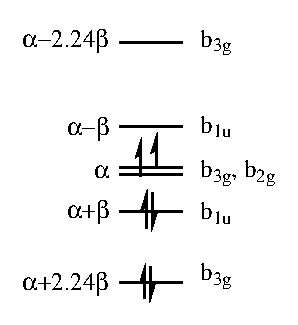
\includegraphics[width=6cm]{huckel2}
	\centering
	\caption{There are a total of 6 $p_{\pi}$ electrons in the system, with atoms 3 and 4 formally radicals.}
	\label{fig:huckel2}
\end{figure}
And we define the \emph{delocalisation energy} as
\begin{defi}[Delocalisation energy]
The delocalisation energy is the difference between the energy of the fully delocalised system and the putative system where only localised double bonds exist.
\end{defi}
So for this system, as we have seen, a localised double bond MO between the same element have two levels, $E=\alpha+\beta$ and $E=\alpha-\beta$, so a two-electron bond have $2\beta+2\beta$. In the localised version of this system, there are two two-electron double bonds and two radical atoms, which just have energies of $\alpha$, so the delocalisation energy is
\begin{equation}
	E_{\text{delocalisation}}=E_{\text{delocalised}}-E_{\text{localised}}=6\alpha+2(\sqrt{5}+1)\beta-(6\alpha+4\beta)\approx2.47\beta
\end{equation}
\section{Perturbation theory}
\subsection{Nondegenerate theory}
Say we are unable to solve
\begin{equation}
H\psi=E\psi,
\end{equation}
however we do have exact solutions for
\begin{equation}
H^{(0)}\psi_n^{(0)}=E_n^{(0)}\psi_n^{(0)}, 
\end{equation}
where $H^{(0)}$ should be broadly functionally similar to $H$. 
We omit the subscript $n$ for now for simplicity's sake. 
This means we can write the original Hamiltonian as $H^{(0)}$ and the difference:
\begin{equation}
H=H^{(0)}+\lambda H',
\end{equation}
where the first term is called the \textbf{unperturbed Hamiltonian} and the 
difference is called the \textbf{perturbation}. $\lambda$ is simply a 
dimensionless parameter running from $0$ to $1$, and it should be small for the 
perturbed system to resemble the unperturbed system. We therefore hope to solve
\begin{equation}
(H^{(0)}+\lambda H')\psi=E\psi.
\end{equation}
If $\lambda$ is small, we can write 
\begin{subequations}
\begin{align}
\psi&=\psi^{(0)}+\lambda\psi^{(1)}+\lambda^2\psi^{(2)}+\cdots\\
E&=E^{(0)}+\lambda E^{(1)}+\lambda^2E^{(2)}+\cdots, 
\end{align}
\end{subequations}
where, formally (added for clarity, rarely used)
\begin{subequations}
\begin{align}
E^{(k)}&=\frac{1}{k!}\diff[k]{E^{(0)}}{\lambda}\Big|_{\lambda=0}\\
\psi^{(k)}&=\frac{1}{k!}\diff[k]{\psi^{(0)}}{\lambda}\Big|_{\lambda=0}.
\end{align}
\end{subequations}
So, the \sch has now become
\begin{equation}
\begin{aligned}
(H^{(0)}+\lambda H')&(\psi^{(0)}+\lambda\psi^{(1)}+\lambda^2\psi^{(2)}+\cdots)\\
=(E^{(0)}+\lambda E^{(1)}+\lambda^2E^{(2)}+\cdots)&(\psi^{(0)}+\lambda\psi^{(1)}+\lambda^2\psi^{(2)}+\cdots).
\end{aligned}
\end{equation}
Expanding and collecting like terms of $\lambda$ we have 
\begin{subequations}
\begin{align}
&H^{(0)}\psi^{(0)}=E^{(0)}\psi^{(0)}\ (\lambda^0\ \text{terms})\\
&H^{(0)}\psi^{(1)}+H'\psi^{(0)}=E^{(0)}\psi^{(1)}+E^{(1)}\psi^{(0)}\ (\lambda^1\ \text{terms})\label{1stpert}\\
&\cdots\nonumber
\end{align}
\end{subequations}
\Cref{1stpert} reads, in bra-ket notation
\begin{equation}
\label{h0h1}
H^{(0)}|\psi^{(1)}\rgl+H'|\psi^{(0)}\rgl=E^{(0)}|\psi^{(1)}\rgl+E^{(1)}|\psi^{(0)}\rgl.
\end{equation}
Multiplying with the bra $\lgl\psi^{(0)}$ we have
\begin{equation}
\begin{aligned}
\lgl\psi^{(0)} |H^{(0)}\psi^{(1)}\rgl+\lgl\psi^{(0)} |H'\psi^{(0)}\rgl&=E^{(0)}\lgl\psi^{(0)} |\psi^{(1)}\rgl+E^{(1)}\lgl\psi^{(0)} |\psi^{(0)}\rgl\\
\lgl H^{(0)}\psi^{(0)} |\psi^{(1)}\rgl+\lgl\psi^{(0)} |H'\psi^{(0)}\rgl&=E^{(0)}\lgl\psi^{(0)} |\psi^{(1)}\rgl+E^{(1)}\\
E^{(1)}&=\lgl\psi^{(0)} |H'\psi^{(0)}\rgl, 
\end{aligned}
\end{equation}
where in the second line we have use the hermiticity of the Hamiltonian. 
We now have the theorem
\begin{thrm}[First-order perturbation theory]
\label{1stpert}
For known perturbed operator $H'$ and known unperturbed eigenfunction 
$\psi^{(0)}$, the first-order correction in energy, $E^{(1)}$ is given by
\begin{equation}
E^{(1)}=\lgl \psi^{(0)}|H'\psi^{(0)}\rgl.
\end{equation}
\end{thrm}
We now have the energy correction, what about the correction in wavefunction? We rewrite \Cref{h0h1} as 
\begin{equation}
\label{1stpertrew}
(H^{(0)}-E^{(0)}_n)\psi^{(1)}_n=-(H'-E^{(1)}_n)\psi_n^{(0)}, 
\end{equation}
where we have added the $n$ subscript where it did not really matter before. 
This is essentially an inhomoheneous differential equation for $\psi_n^{(1)}$. 
We try expanding $\psi_n^{(1)}$ in $\psi_n^{(0)}$'s as we know they form a 
complete set: 
\begin{equation}
\psi^{(1)}_n=\sum_{m\neq n}c_m^{(n)}\psi^{(0)}_m.
\end{equation}
We need to exclude the $m=n$, \ie $\psi^{(0)}_n$ term because the normalisation 
requirement for $\psi_n$ requires that
\begin{equation}
1=\lgl \psi_n|\psi_n\rgl=\lgl \psi^{(0)}_n |\psi^{(0)}_n\rgl+\lambda(\lgl\psi^{(1)}_n|\psi^{(0)}_n\rgl+\lgl \psi^{(0)}_n|\psi^{(1)}_n\rgl)+\lambda^2(\cdots)+\cdots,
\end{equation}
but since the first term of the sum must be $1$ due to orthonormality of the 
unperturbed state, the subsequent terms must be zero, which means 
\begin{equation}
\label{pertorth}
\lgl \psi^{(1)}_n|\psi^{(0)}_n\rgl=0, 
\end{equation}
which means $\psi^{(1)}_n$ cannot contain a $\psi^{(0)}_n$ term. Now putting this 
into \Cref{1stpertrew} we get
\begin{equation}
\begin{aligned}
\sum_{m\neq n}(E_m^{(0)}-E_n^{(0)})c_m^{(n)}\psi_m^{(0)}&=-(H'-E_n^{(1)})\psi_n^{(0)}\\
\sum_{m\neq n}(E_m^{(0)}-E_n^{(0)})c_m^{(n)}\lgl\psi_l^{(0)}|\psi_m^{(0)}\rgl&=-\lgl\psi_l^{(0)}|H'\psi_n^{(0)}\rgl+E_n^{(1)}\lgl\psi_l^{(0)}|\psi_n^{(0)}\rgl
\end{aligned}
\end{equation}
If we set $l=n$ we recover the energy correction since the left side will return 
zero. But if $l\neq n$, we get
\begin{equation}
(E_l^{(0)}-E_n^{(0)})c_l^{(n)}=-\lgl\psi_l^{(0)} |H'\psi_n^{(0)} \rgl, 
\end{equation}
which gives us expression for the $c_m^{(n)}$'s (by relabelling) and so we have what we're looking for: 
\begin{thrm}[First-order correction in wavefunction]
\begin{equation}
\psi_n^{(1)}=\sum_{m\neq n}\frac{\lgl\psi_m^{(0)} |H'\psi_n^{(0)} \rgl}{(E_n^{(0)}-E_m^{(0)})}\psi_m^{(0)}.
\end{equation}
\end{thrm}
Going one power higher we have
\begin{equation}
\begin{aligned}
H^{(0)}\psi_n^{(2)}+H'\psi_n^{(1)}&=E_n^{(0)}\psi_n^{(2)}+E_n^{(1)}\psi_n^{(1)}+E_n^{(2)}\psi_n^{(0)}\\
\lgl\psi_n^{(0)}|H^{(0)}\psi_n^{(2)}\rgl+\lgl\psi_n^{(0)}|H'\psi_n^{(1)}\rgl&=E_n^{(0)}\lgl\psi_n^{(0)}|\psi_n^{(2)}\rgl+E_n^{(1)}\lgl\psi_n^{(0)}|\psi_n^{(1)}\rgl+E_n^{(2)}\lgl\psi_n^{(0)}|\psi_n^{(0)}\rgl\\
E_n^{(0)}\lgl\psi_n^{(0)}|\psi_n^{(2)}\rgl+\lgl\psi_n^{(0)}|H'\psi_n^{(1)}\rgl&=E_n^{(0)}\lgl\psi_n^{(0)}|\psi_n^{(2)}\rgl+E_n^{(1)}\lgl\psi_n^{(0)}|\psi_n^{(1)}\rgl+E_n^{(2)}\\
E_n^{(2)}&=\lgl\psi_n^{(0)}|H'\psi_n^{(1)}\rgl-E_n^{(1)}\lgl\psi_n^{(0)}|\psi_n^{(1)}\rgl
\end{aligned}
\end{equation}
but as we have already seen in \Cref{pertorth}, the second term shall be zero, so
\begin{equation}
\begin{aligned}
E_n^{(2)}&=\sum_{m\neq n}c_m^{(n)}\lgl \psi_n^{(0)} |H'\psi_m^{(0)} \rgl \\
&=\sum_{m\neq n}\frac{\lgl\psi_m^{(0)} |H'\psi_n^{(0)} \rgl\lgl\psi_n^{(0)} |H'\psi_m^{(0)} \rgl}{E_n^{(0)}-E_m^{(0)}}\\
&=\sum_{m\neq n}\frac{|\lgl\psi_m^{(0)} |H'\psi_n^{(0)} \rgl|^2}{E_n^{(0)}-E_m^{(0)}}
\end{aligned}
\end{equation}
\begin{thrm}[Second-order energy correction]
\label{2ndecorr}
\begin{equation}
E_n^{(2)}=\sum_{m\neq n}\frac{|\lgl\psi_m^{(0)} |H'\psi_n^{(0)} \rgl|^2}{E_n^{(0)}-E_m^{(0)}}.
\end{equation}
\end{thrm}
Now, all of this will crumble if $E_n^{(0)}=E_m^{(0)}$, \ie if there are two 
\textbf{degenerate} unperturbed states. We will discuss it after we look at some 
examples. 
\subsection{Examples}
\textbf{Anharmonic oscillators}\\
The Hamiltonian is now given by 
\begin{equation}
H=\underbrace{-\frac{\hbar^2}{2\mu}\diff[2]{}{x}+\frac{1}{2}kx^2}_{H^{(0)}}\underbrace{\vphantom{-\frac{\hbar^2}{2\mu}\diff[2]{}{x}+\frac{1}{2}kx^2}+\frac{1}{6}\gamma x^3+\frac{1}{24}bx^4}_{H'}.
\end{equation}
And we know that the unperturbed ground wavefunction is
\begin{equation}
\psi^{(0)}(x)=\lf(\frac{\alpha}{\pi}\rt)^{1/4}e^{-\alpha x^2/2}
\end{equation}
where $\alpha=(k\mu/\hbar^2)^{1/2}$. \\
So we apply the first order perturbation theory:
\begin{equation}
\begin{aligned}
E^{(1)}=&\lgl \psi^{(0)}|H'\psi^{(0)} \rgl\\
=&\lf(\frac{\alpha}{\pi}\rt)^{1/2}\bigg[\frac{\gamma}{6}\underbrace{\intinf x^3e^{-\alpha x^2}\dx}_{\text{odd integrand, }0}+\frac{b}{24}\intinf x^4e^{-\alpha x^2}\dx \bigg]\\
=&\frac{b}{32\alpha^2}=\frac{\hbar^2b}{32k\mu}, 
\end{aligned}
\end{equation}
where we have used the standard integral. So the first order ground-state energy is 
\begin{equation}
E=\frac{1}{2}\hbar\omega+\frac{1}{32}\frac{\hbar^2b}{k\mu}.
\end{equation}
\ \\
\textbf{Helium ground state (again)}\\
The unperturbed Hamiltonian is 
\begin{equation}
H^{(0)}=H_1+H_2
\end{equation}
where the $H_i$'s are $Z=2$ hydrogenlike Hamiltonians, and the unperturbed ground state and energy are
\begin{equation}
\begin{aligned}
\psi^{(0)}=\psi_{1s}(r_1,\theta_1,\phi_1)\psi_{1s}(r_2,\theta_2,\phi_2)\\
E^{(0)}=-\frac{Z^2}{2}-\frac{Z^2}{2},
\end{aligned}
\end{equation}
and the perturbed Hamiltonian is 
\begin{equation}
H'=\frac{e^2}{4\pi\ep r_{12}}.
\end{equation}
Applying the theory we have
\begin{equation}
E^{(1)}=\iint\psi_{1s}(\bvec{r}_1)\psi_{1s}(\bvec{r}_2)\frac{e^2}{4\pi\ep r_{12}}\psi_{1s}(\bvec{r}_1)\psi_{1s}(\bvec{r}_2)\dif\bvec{r}_1\dif\bvec{r}_2=\frac{5}{8}Z,
\end{equation}
where we have used the same result from \Cref{5z8}. So the first-order energy is 
\begin{equation}
E=-Z^2+\frac{5}{8}Z=-2.75.
\end{equation}
Slightly worse than the variational calculation we did earlier, but with higher 
order corrections the energy will become highly accurate. 
\subsection{Degenerate theory}
This section draws heavily from L2.3-3.2 of \cite{bartonyt} in conjunction with 
its accompanying notes (\cite{barton}) and also Section 6.8 of \cite{atkinsqm}.\par
Now suppose we have an $N$-fold degeneracy of the \textit{unperturbed} 
wavefunction, which is to say, for $1<k<N$
\begin{equation}
H^{(0)}|n^{(0)},k\rgl=E^{(0)}|0,k\rgl, 
\end{equation}
this is the same as saying that $H^{(0)}$ is, in the basis of the eigenstate, 
a diagonal matrix with digonal entries
\begin{equation}
H^{(0)}=\text{diag}\{E_1^{(0)},E_2^{(0)},\cdots,\underbrace{E_n^{(0)},\cdots,E_n^{(0)}}_{N},\cdots \}.
\end{equation}
In the \textit{degenerate subspace}, $\mathbb{V}_N$, we choose a collection of 
$N$ \textit{orthonormal} eigenstates
\begin{equation}
|n^{(0)};1\rgl,|n^{(0)};2\rgl,\cdots,|n^{(0)};N\rgl.
\end{equation}
The other states outside the subspace may also contain degeneracy but we do not 
have to be concerned with them, since they have \textit{different energy} than 
\textit{these} degenerate states, and so do not pose problems in the denominator, 
so to say. We label this space $\hat{V}$, with eigenvectors (and since $H^{(0)}$ 
is diagonal in $\hat{V}$, the basis vectors) $|p^{(0)}\rgl $. 
Compactly put, the total state space (Hilbert space) is
\begin{equation}
\mathcal{H}=\mathbb{V}_N\oplus\hat{V}.
\end{equation}
We will use the following orthonormality conditions: 
\begin{prt}[Orthonormality conditions of DPT]
\label{dptorth}
\begin{equation}
\lgl p^{(0)} |q^{(0)} \rgl=\delta_{pq},\ \lgl p^{(0)} |n^{(0)};k \rgl=0,\ \lgl n^{(0)};k |n^{(p>0)};k \rgl=0,
\end{equation}
\end{prt}
where the third is due to \Cref{pertorth} again, which intuitively says that the 
higher order terms receive no correction from the ground state, because it can 
just be reabsorbed into the normalisation of the ground state (just a restatement 
of the justification of \Cref{pertorth}). 
However note that it can receive correction from \textit{other} degenerate states, 
\ie $\lgl n^{(0)};k |n^{(p>0)};k \rgl$ is not necessarily zero.\par
In the most general terms, when the perturbation ($\lambda$) is turned on, 
the degenerate states and their energies will become
\begin{equation}
\begin{aligned}
|n^{(0)};k\rgl\rightarrow|n;k\rgl_{\lambda}&\equiv|n^{(0);k}+\lambda|n^{(1)};k\rgl+\lambda^2|n^{(2)};k\rgl+O(\lambda^3)\\
E_n^{(0)}\rightarrow E_{n,k}(\lambda)&\equiv E_n^{(0)}+\lambda E_{n,k}^{(1)}+\lambda^2 E_{n,k}^{(2)}+O(\lambda^3)
\end{aligned}
\end{equation}
Now, we say that the degeneracy is \textit{lifted} in the first order if all 
$E_{n,k}^{(1)}$ has different values, \ie they have now diverged and can be told apart. 
Our goal is find these corrections and then the first-order corrections in the 
eigenvector, $|n^{(1)};k\rgl $, for all $k$. \par
To cast this in the eigenfunction language we've used for the nondegenerate case, this is 
to say that we will determine the linear combinations of $\psi^{(0)}_k$'s that make up 
$\psi^{(1)}_k$, and implicitly in this we also need to find an 
\textit{appropriate set} of $\psi^{(0)}_k$'s such that our final linear 
combinations will be as simple as possible.\par
The \sch to solve is
\begin{equation}
H(\lambda)|n;k\rgl_{\lambda}=E_{n,k}(\lambda)|n;k\rgl_{\lambda},
\end{equation}
where
\begin{equation}
H(\lambda)=H^{(0)}+\lambda H',
\end{equation}
is just our Hamiltonian with perturbation as before. We'll extract our equations 
in ascending orders of $\lambda$ exactly as before: 
\begin{subequations}
\begin{align}
&\lambda^0:(H^{(0)}-E_n^{(0)})|n^{(0)};k\rgl=0,\\
&\lambda^1:(H^{(0)}-E_n^{(0)})|n^{(1)};k\rgl=(E_{n,k}^{(1)}-H')|n^{(0)};k\rgl ,\\
&\lambda^2:(H^{(0)}-E_n^{(0)})|n^{(2)};k\rgl=(E_{n,k}^{(1)}-H')|n^{(1)};k\rgl+E_{n,k}^{(2)}|n^{(0)};k\rgl,\\
&\cdots\nonumber
\end{align}
\end{subequations}
The $\lambda^0$ equation is trivial, and we can ignore it. Now we have a 
three-step plan to solve our problem at hand:
\begin{enumerate}
	\item Right-multiply the $\lambda^1$ equation with $\lgl n^{(0)};l|$, conclude condition that the choice of basis must fulfill.
	\item Use the $\lambda^1$ equation to get the components of $|n^{(1)};k\rgl$ in $\hat{V}$.
	\item Right-multiply the $\lambda^2$ equation with $\lgl n^{(0)};l|$ to get the second order energy correction $E^{(2)}_{n,k} $ and the component of $\lgl n^{(0)};l|$ in $\mathbb{V}_N$.
\end{enumerate}
\textbf{Step 1}\\
The LHS is simply zero due to the orthonormality condition and the hermiticity of $H^{(0)}$. \par
The RHS yields
\begin{equation}
\label{6240}
\lgl n^{(0)};l|(E^{(1)})_{n,k}-H'|n^{(0)};k \rgl=0\ \imp\ 
(H')_{lk}=E_{n,k}^{(1)}\delta_{lk}
\end{equation}
Now this equation tells us several very important things, the most important being
\begin{thrm}[Diagonalisation of $H'$]
$H'$ is diagonalised in $\mathbb{V}_N$, and the first order correction in energy is 
\begin{equation}
E_n^{(1)}=(H')_{nk,nk}, 
\end{equation}
the diagonal entries of $H'$ \textit{in the choice of basis} in 
$\mathbb{V}_N$ that diagonalises $H'$. The $n$ subscript is just to 
remind us that there's an $n$-fold degeneracy. 
\end{thrm}
There are three additional remarks:
\begin{enumerate}
	\item We have only shown that $H'$ is diagonalised in $\mathbb{V}_N$ \textit{only}, it is \textbf{not} diagonalised on the entire Hilbert space $\mathcal{H}$, \ie the basis vectors $|n^{(0)};k$ are eigenvectors only in $\mathbb{V}_N$ not $\mathcal{H}$. We can see this by inserting a resolution of identity:
	\begin{equation}
	\begin{aligned}
	H'|n^{(0)};l\rgl\Big|_{\mathcal{H}}&=\sum_q |n^{(0)};q\rgl \lgl n^{(0)};q |H'|n^{(0)};l \rgl\Big|_{\mathbb{V}_N}+\sum_p |p^{(0)}\rgl \lgl p^{(0)}|H' |n^{(0)};l \rgl\Big|_{\hat{V}}\\
	&=\sum_q E_{n,l}^{(1)}\delta_{lq}|n^{(0)};q\rgl+\sum_p |p^{(0)}\rgl \lgl p^{(0)}|H' |n^{(0)};l \rgl\\
	&=E_{n,l}^{(1)}|n^{(0)};l\rgl+\sum_p |p^{(0)}\rgl \lgl p^{(0)}|H' |n^{(0)};l \rgl
	\end{aligned}
	\end{equation}
	If we only resolved the identity in $\mathbb{V}_N$ we will have gotten the first term only, which means that it's diagonalised in it. The second term means that $|n^{(0)};k\rgl$ indeed have components along $\hat{V}$, \ie it receives contribution from other states, which intuitively makes sense. 
	\item As we can see, we can \textit{only} determine the energy correction if $H'$ is diagonalised. This requires the choice of a `good' basis set of $|n^{(0)};k\rgl$'s, as alluded to before. If we fail to choose a good basis set we just have to manually diagonalise it. 
	\item This relates to the above point, we can utilise a theorem, introduced below to determine if $H'$ is diagonal without much computation. If it's not, however, we'll have to manually diagonalise it, which will be discussed below. 
\end{enumerate}
\begin{thrm}[Quick determination of whether $H'$ diagonalises]
The matrix $H'$ is diagonal for a choice of basis in $\mathbb{V}_N$ if there is a 
Hermitian operator $K$ that commutes with $H'$ for which the chosen basis vectors are 
eigenstates of $K$ with \textit{different} eigenvalues. 
\end{thrm}
\begin{proof}
Let $[H',K]=0$ and that for two basis states in $\mathbb{V}_N$, $|n^{(0)};p\rgl$ and $|n^{(0)};q\rgl$ we have eigenvalues of $K$, $\lambda_p\neq\lambda_q$, so we have
\begin{equation}
0=\lgl n^{(0)};p|[H',K]|n^{(0)};q \rgl=\underbrace{(\lambda_p-\lambda_q)}_{\neq0}\lgl n^{(0)};p|H'|n^{(0)};q \rgl.
\end{equation}
Therefore the off-diagonal entries of $H'$ must vanish. 
\end{proof}
Now, if we weren't so lucky to choose an orthonormal basis, all we need to do is to examine the elements of $H'$ in $\mathbb{V}_N$ and calculate the roots of the 
\textit{characteristic equation}, which we can then use to diagonalise the matrix. \par
\textbf{Step 2}\\
We now determine the components of $|n^{(1)};k\rgl$ along $\hat{V}$, whose basis vectors 
are $\rgl p^{(0)}|$, so we right-multiply it to the equation to find
\begin{equation}
\begin{aligned}
\lgl p^{(0)} | (H^{(0)}-E_n^{(0)})|n^{(1)};k \rgl\Big|_{\hat{V}}&=-\lgl p^{(0)} | H'|n^{(0)};k \rgl\\
(E_p^{(0)}-E_n^{(0)})\lgl p^{(0)} | n^{(1)};k \rgl\Big|_{\hat{V}}&=-(H')_{p,nk}\\
|n^{(1)};k\rgl\Big|_{\hat{V}}&=-\sum_p\frac{(H')_{p,nk}}{E_p^{(0)}-E_n^{(0)}}|p^{(0)}\rgl\\
|n^{(1)};k\rgl=|n^{(1)};k\rgl\Big|_{\mathbb{V}_N}+|n^{(1)};k\rgl\Big|_{\hat{V}}&=-\sum_p\frac{(H')_{p,nk}}{E_p^{(0)}-E_n^{(0)}}|p^{(0)}\rgl+|n^{(1)};k\rgl\Big|_{\mathbb{V}_N}
\end{aligned}
\end{equation}
\textbf{Step 3}\\
Now we want to find the components in the degenerate space, so we right-multiply the 
$\lambda^3$ equation with the basis vectors $\lgl n^{(0)};l|$:
\begin{equation}
\begin{aligned}
0=&\lgl n^{(0)};l | (E^{(1)}_{nk}-H')|n^{(1)};k \rgl+E^{(2)}_{nk}\delta_{kl}\\
=&-\lgl n^{(0)};l | (E^{(1)}_{nk}-H')\sum_p|p^{(0)} \rgl\frac{(H')_{p,nk}}{E_p^{(0)}-E_n^{(0)}}\\
&+\lgl n^{(0)};l | (E^{(1)}_{nk}-H')|n^{(1)};k \rgl\Big|_{\mathbb{V}_N}+E^{(2)}_{nk}\delta_{kl}\\
=&\lgl n^{(0)};l | H'\sum_p|p^{(0)} \rgl\frac{(H')_{p,nk}}{E_p^{(0)}-E_n^{(0)}}+\lgl n^{(0)};l | (E^{(1)}_{nk}-H')|n^{(1)};k \rgl\Big|_{\mathbb{V}_N}+E^{(2)}_{nk}\delta_{kl}\\
=&\sum_p\frac{(H')_{nl,p}(H')_{p,nk}}{E_p^{(0)}-E_n^{(0)}}+\lgl n^{(0)};l | (E^{(1)}_{nk}-H')|n^{(1)};k \rgl\Big|_{\mathbb{V}_N}+E^{(2)}_{nk}\delta_{kl}.
\end{aligned}
\end{equation}
To simply this expression further we insert a resolution of identity in the second term
\begin{equation}
\begin{aligned}
&\lgl n^{(0)};l | H'|n^{(1)};k \rgl\Big|_{\mathbb{V}_N}\\
=&\underbrace{\lgl n^{(0)};l | H'|\bigg(\sum_q|n^{(0)};q \rgl}_{(H')_{nl,nq}} \lgl n^{(0)};q+\sum_p|p^{(0)}\rgl\underbrace{\vphantom{\bigg(\sum_q}\lgl p^{(0)}| \bigg)|n^{(1)};k\rgl\Big|_{\mathbb{V}_N}}_{\hat{V}\perp\mathbb{V}_N\ \imp\ 0}\\
=&\sum_q E^{(1)}_{nl}\delta_{lq}\lgl n^{(0)};q | n^{(1)};k \rgl\Big|_{\mathbb{V}_N}.
\end{aligned}
\end{equation}
So we obtain the `master' equation:
\begin{equation}
\underbrace{-\sum_p\frac{(H')_{nl,p}(H')_{p,nk}}{E_p^{(0)}-E_n^{(0)}}+(E_{nk}^{(1)}-E_{nl}^{(1)})}_{\text{known quantities}}\underbrace{\vphantom{-\sum_p\frac{(H')_{nl,p}(H')_{p,nk}}{E_p^{(0)}-E_n^{(0)}}}\lgl n^{(0)};l | n^{(1)};k \rgl\Big|_{\mathbb{V}_N}}_{\text{main unknown}}+E_{nk}^{(2)}\delta_{lk}=0.
\end{equation}
This equation is quite rich in information: we can obtain the second-order energy 
correction if we set $l=k$, which elimintates our main unknown due to the third 
orthonormality condition. When we set $l\neq	k$ the second-order energy disappears, 
leaving us a simpler expression for our main unknown.
\begin{thrm}[Second-order energy correction, degenerate]
When $l=k$, we immediately obtain
\begin{equation}
\begin{aligned}
E^{(2)}_{nk}&=\lgl n^{(0)};k | H'|n^{(1)};k \rgl\Big|_{\hat{V}}\\
&=-\sum_p\frac{|(H')_{nk,p}|^2}{E_p^{(0)}-E_n^{(0)}},
\end{aligned}
\end{equation}
We see that it's the same form as the nondegenerate case (\Cref{2ndecorr}), 
only that the sum is over outside the degenerate space. 
\end{thrm}
As an aside, if we believed naively that there are no components inside the degenerate 
space, we would have concluded that
\begin{equation}
\lgl n^{(0)};l | H'|n^{(1)};k \rgl\Big|_{\hat{V}}=0, 
\end{equation}
which we have shown to be not zero. \par
Finally, we set $l\neq k$ to get
\begin{equation}
\begin{aligned}
\lgl n^{(0)};l | n^{(1)};k \rgl\Big|_{\mathbb{V}_N}&=\frac{1}{E_{nk}^{(1)}-E_{nl}^{(1)}}\lgl n^{(0)};l | H'|n^{(1)};k \rgl\Big|_{\hat{V}}\\
&=-\frac{1}{E_{nk}^{(1)}-E_{nl}^{(1)}}\sum_p\frac{(H')_{nl,p}(H')_{p,nk}}{E_p^{(0)}-E_n^{(0)}},\ l\neq k
\end{aligned}
\end{equation}
The fraction implies that the degeneracy must be \textit{completely} lifted, otherwise 
we must resolve the degeneracy to higher orders. Projecting along the basis we have
\begin{equation}
|n^{(1)};k\rgl\Big|_{\mathbb{V}_N}=-\sum_{l\neq k}|n^{(0)};k\rgl\frac{1}{E_{nk}^{(1)}-E_{nl}^{(1)}}\sum_p\frac{(H')_{nl,p}(H')_{p,nk}}{E_p^{(0)}-E_n^{(0)}}.
\end{equation}
Curiously the degenerate corrections depend on the nondegenerate corrections. In all, 
\begin{thrm}[First-order correction to eigenfunction, degenerate]
\begin{equation}
\begin{aligned}
|n^{(1)},k\rgl&=|n^{(1)},k\rgl\Big|_{\mathbb{V}_N}+|n^{(1)},k\rgl\Big|_{\hat{V}}\\
&=-\sum_{l\neq k}|n^{(0)};k\rgl\frac{1}{E_{nk}^{(1)}-E_{nl}^{(1)}}\sum_p\frac{(H')_{nl,p}(H')_{p,nk}}{E_p^{(0)}-E_n^{(0)}}-\sum_p\frac{(H')_{p,nk}}{E_p^{(0)}-E_n^{(0)}}|p^{(0)}\rgl
\end{aligned}
\end{equation}
\end{thrm}
\section{The Hartree-Fock method}
\subsection{Self-consistent field method}
\label{scf}
A more inspired trial function for the variational method could be the 
\textbf{Slater orbitals}, given by 
\begin{equation}
S_{nlm}(r,\theta,\phi)=Nr^{n-1}e^{-\zeta r}Y^m_l(\theta,\phi),
\end{equation}
where $\zeta$ is a variational parameter and
\begin{equation}
N=\frac{(2\zeta)^{n+1/2}}{\sqrt{(2n)!}}.
\end{equation}
There is no inclusion of the Legendre polynomial so there are't any radial nodes, 
and as a consequence these orbitals aren't in general orthogonal. \\
Now the starting point of the Hartree-Fock procedure for helium is to write the 
two-electron wavefunction as a product of two orbitals, typically linear 
combinations of slater orbitals:
\begin{equation}
\psi(\bvec{r}_1,\bvec{r}_2)=\phi(\bvec{r}_1)\phi(\bvec{r}_2).
\end{equation}
The two one-electron wavefunctions are the same, which is \textit{in direct violation} of the Pauli exclusion principle. We ignore it for the moment. 
We must try to account for the interelectronic repulsion in the Hamiltonian:
\begin{equation}
\label{hfham}
H_1=-\frac{1}{2}\onabla_1^2-\frac{2}{r}+V_1^{\text{eff}}(r_1),
\end{equation}
where we have adopted atomic units and where the effective potential is where we 
introduce interelectronic repulsion as an average potential (this is also known as 
the \textit{mean field approximation}):
\begin{equation}
V^{\text{eff}}_1(r_1)=\lgl \phi(\bvec{r}_2)|\frac{1}{r_{12}}|\phi(\bvec{r}_2)\rgl.
\end{equation}
Now we have our \sch
\begin{equation}
H_1\phi(\bvec{r}_1)=\epsilon_1\phi(\bvec{r}_1).
\end{equation}
This is called the \textbf{Hartree-Fock equation} for a Helium atom. A special 
feature of the equation is that its Hamiltonian depends on $\phi(\bvec{r}_2)$ 
through \Cref{hfham}. $\phi(\bvec{r}_2)$ in turn is the exact same function as the 
solution of the equation, $\phi(\bvec{r}_1)$. This recursive relation allows for 
iteration and that's the essence of the \textbf{self-consistent field method}: we 
first guess a form, any form, for $\phi(\bvec{r}_2)$ and evaluate the effective 
potential, and hence the Hamiltonian, and we solve the \sch for $\phi(\bvec{r}_1)$
, by \hl{todo/todo-supo: check if by variational principle or perturbation theory}, and use the output as the 
input again, until the output is sufficiently close to the input, or \textit{
self-consistent}. 
\subsection{Accounting for spin}
\label{acc_for_spin}
In treating the helium atom just now we only used the spatial part of the trial 
wavefunction, and it appeared to have contradicted Pauli exclusion principle. 
But we have not, we just need to say that the two electrons must be in the 
singlet configuration, which is antisymmetric wrt electron exchange. The spin 
does not contribute anything to any integrals involving spatial integration 
as the Hamiltonian does not depend on it\footnote{This is again assuming spin and 
orbitals are uncoupled.} and that they are made orthonormal. \\
However, all this triplet and singlet talk is when we only have two electrons, 
what if we need to construct antisymmetric wavefunctions out of $N$-electrons? 
We introduce the 
\begin{defi}[Slater determinant]
We can use the Slater determinant to construct antisymmetric $N$-electron wavefunctions:
\begin{equation}
\ups(1,2,\cdots,N)=\frac{1}{\sqrt{N!}}
\begin{vmatrix}
u_1(1)&u_2(1)&\cdots&u_N(1)\\
u_1(2)&u_2(2)&\cdots&u_N(2)\\
\vdots&\vdots&\ddots&\vdots\\
u_1(N)&u_2(N)&\cdots&u_N(N)
\end{vmatrix}, 
\end{equation}
where $u_i(j)$ are the $i$-th complete (\ie spin included) orthonormal orbitals 
for particle $j$. 
\end{defi} 
The determinant works because
\begin{enumerate}
	\item It changes signs whenever two electrons (rows) are swapped; 
	\item It vanishes whenever two electrons occupy the same state (two identical columns). 
\end{enumerate}
For example, we look at the lithium atom. The intuition tells us to try 
\begin{equation}
\psi(\bvec{r}_1,\bvec{r}_2,\bvec{r}_3)=\phi_{1s}(\bvec{r}_1)\phi_{1s}(\bvec{r}_2)\phi_{1s}(\bvec{r}_3), 
\end{equation}
but we the Pauli exclusion principle says we can't possibly accomodate three 
electrons in the $1s$ orbital, and we put our electron in the next lowest energy 
orbital\footnote{This is still just to construct a trial wavefunction because we don't know for sure what the energy level is like for lithium atoms, but it's the best guess we've got.}, the $2s$, and construct the antisymmetric wavefunction as follows:
\begin{equation}
\psi=\frac{1}{\sqrt{3!}}
\begin{vmatrix}
1s\alpha(1)&1s\beta(1)&2s\alpha(1)\\
1s\alpha(2)&1s\beta(2)&2s\alpha(2)\\
1s\alpha(3)&1s\beta(3)&2s\alpha(3)
\end{vmatrix}, 
\end{equation}
where $1s$ is shorthand for $\psi_{1s}$ and $\alpha$ is shorthand for spin-up and $\beta$ for spin-down. \\
Now let's treat the first excited state of helium, $1s^12s^1$. \\
First we introduce a more compact notation\cite{hughbanks}:
\begin{equation}
1s\equiv1s\alpha,\ \overline{1s}\equiv1s\beta
\end{equation}
and
\begin{equation}
|1s\ \overline{2s}|\equiv N
\begin{vmatrix}
1s(1)&\overline{2s}(1)\\
1s(2)&\overline{2s}(2)\\
\end{vmatrix}, 
\end{equation}
where the normalisation constant is implied. 
Now let's construct the antisymmetric wavefunctions: 
\begin{equation}
|1s\ 2s|=\frac{1}{\sqrt{2}}
\begin{vmatrix}
1s\alpha(1)&2s\alpha(1)\\
1s\alpha(2)&2s\alpha(2)
\end{vmatrix}\propto[1s(1)2s(2)-2s(1)1s(2)](\uparrow\uparrow)\ (^3\ups,\ M_s=+1)
\end{equation}
\begin{equation}
|1s\ \overline{2s}|=\frac{1}{\sqrt{2}}
\begin{vmatrix}
1s\alpha(1)&2s\beta(1)\\
1s\alpha(2)&2s\beta(2)
\end{vmatrix}\propto1s(1)2s(2)\uparrow\downarrow-2s(1)1s(2)\downarrow\uparrow
\end{equation}
Now this is a state with $M_s=0$ according to \Cref{add_zmom}, if we combine a particle 
with spin up and one with spin down we get zero $z$-momentum. And here's one more
\begin{equation}
|\overline{1s}\ 2s|\propto1s(1)2s(2)\downarrow\uparrow-2s(1)1s(2)\uparrow\downarrow.
\end{equation}
Now, this is the \textbf{decoupled picture}, in which $m$, the $z$-spin momenta 
are specified, which is a perfectly legitimate way to specify the system, but we 
would like to speak of `singlet' and `triplet', \ie of the \textbf{coupled 
picture} where $s$, the total spin momentum is specified, to do so we take the 
linear combination of our states:
\begin{equation}
\begin{aligned}
&\frac{1}{\sqrt{2}}(|1s\ \overline{2s}|+|\overline{1s}\ 2s|)=[1s(1)2s(2)-2s(1)1s(2)](\uparrow\downarrow+\downarrow\uparrow)\ (^3\ups,\ M_s=0) \\
&\frac{1}{\sqrt{2}}(|1s\ \overline{2s}|-|\overline{1s}\ 2s|)=[1s(1)2s(2)-2s(1)1s(2)](\uparrow\downarrow-\downarrow\uparrow)\ (^1\ups,\ M_s=0)
\end{aligned}
\end{equation}
The last state is
\begin{equation}
|\overline{1s}\ \overline{2s}|\propto[1s(1)2s(2)-2s(1)1s(2)]\downarrow\downarrow\ (^3\ups, M_s=-1).
\end{equation}
Ok, let's apply first-order perturbation theory to these orbitals. \hl{todo: read atkinsqm on degenerate cases, dk if this is entirely correct, priority: high}:
\begin{equation}
\begin{aligned}
E^{(1)}=&\lgl \ups_{\pm}|\frac{1}{r_{12}}|\ups_{\pm}\rgl\\
=&\frac{1}{2}\lgl1s(1)2s(2)\pm2s(1)1s(2)|\frac{1}{r_{12}}|1s(1)2s(2)\pm2s(1)1s(2)\rgl\\
\equiv&J\pm K, 
\end{aligned}
\end{equation}
where $J$ is the \textbf{Coulomb integral} and $K$ the \textbf{exchange integral} 
(Section 7.9 of \cite{atkinsqm}):
\begin{equation}
\begin{aligned}
J&=\lgl 1s(1)2s(2)|\frac{1}{r_{12}}|1s(1)2s(2)\rgl\\
K&=\lgl 1s(1)2s(2)|\frac{1}{r_{12}}|1s(2)2s(1)\rgl
\end{aligned}
\end{equation}

\subsection{The Hartree-Fock method}
In \Cref{scf} we have discussed the Hartree-Fock method for the helium atom. 
However it is only a special case as the spin and spatial wavefunction neatly 
separates:
\begin{equation}
\ups=\frac{1}{\sqrt{2}}
\begin{vmatrix}
1s\alpha(1)&1s\beta(1)\\
1s\alpha(2)&1s\beta(2)
\end{vmatrix}
=\frac{1}{\sqrt{2}}1s(1)1s(2)(\uparrow\downarrow-\downarrow\uparrow).
\end{equation}
And it is readily seen that the same is impossible for even lithium atom as the the dependences of all the spatial wavefunctions will be permuted. \hl{todo-supo: can we introduce LCs like above?}\\
Now we are ready to introduce the general Hartree-Fock method. Our goal is still the same: to solve the \sch with Hamiltonian (same as in \Cref{genham}):
\begin{equation}
H=\sum_i H^{(0)}(i)+\frac{1}{2}\sum_{i\neq j}\frac{1}{r_{ij}}, 
\end{equation}
where the first term is the \textit{core Hamiltonian} with nuclear charge $Ze$ for 
the $i$-th electron, and the second term is the interelectronic repulsion. 
By using the slater determinant to approximate the orbitals and by using the 
mean-field approximations for effective interelectronic potentials, and through 
some tricky derivation (see pp. 528-531 of \cite{atkinsqm}) the completely general 
Hartree-Fock equation is introduced as follows:
\begin{thrm}[Hartree-Fock equation]
The Hartree-Fock equation for a \textit{spin-orbital}\footnote{The spins will 
produce Kronecker deltas anyway, but it's just more correct to speak of 
spin-orbitals.} $\phi_s(1)$ occupied by electron 1 is 
\begin{equation}
\lf[H^{(0)}(1)+\sum_r(J_r-K_r) \rt]\phi_s(1)=\epsilon_s\phi_s(1),
\end{equation}
where the sum is over all occupied spin-orbitals. 
\end{thrm}
$J$ and $K$ are two operators, defined as follows:
\begin{defi}[Coulomb and exchanger operators]
\ \\
$J_r$ is the \textbf{Coulomb operator}
\begin{equation}
J_r|\phi_s(1)\rgl=\lgl\phi_r(2)|\frac{1}{r_{12}}|\phi_r(2)\rgl|\phi_s(1)\rgl.
\end{equation}
$K_r$ is the \textbf{exchange operator}
\begin{equation}
K_r|\phi_s(1)\rgl=\lgl\phi_r(2)|\frac{1}{r_{12}}|\phi_s(2)\rgl|\phi_r(1)\rgl.
\end{equation}
$J$ accounts for the effect of Coulombic repulsion and $K$, spin correlation. 
\end{defi}
Note that since 
\begin{equation}
J_a(1)|\phi_a(1)\rgl=K_a(1)|\phi_a(1), 
\end{equation}
the sum in the Fock operator correctly gives results for all electron pair interactions without counting the same electron interacting with itself. \\
Now the Fock operator depends on $n$ spin-orbitals, and again we solve the 
Hartree-Fock equation by the self-consistent field method. After that, the 
Fock operator is theoretically a well-defined Hermitian operator and we can 
generate an infinite set of eigenfunctions, but in practice we only solve 
$m\geq n$ optimised spin-orbitals, with the $n$ lowest energy orbitals called 
\textbf{occupied orbitals} and the rest \textbf{virtual orbitals}. The slater 
determinant (or a linear combination of them, to correct the spin symmetry) 
composed with the optimised $n$ occupied orbitals is then the 
HF ground-state wavefunction for the system, $\Phi_0$. \\
The HF-SCF method takes into account spin correlation, however, the Coulombic 
interactions between electrons are treated in an average way, so no instantaneous 
interactions, nor quantum mechanical electron distribution, are taken into 
account. These are collectively called \textbf{electron correlation}, and is 
entirely left out of the picture by the HF-SCF method. 
\chapter{Group theory}
\section{The bare minimum}
\subsection{Symmetry elements and symmetry operations}
\begin{defi}[Symmetry operations]
A \textbf{symmetry operation} is an operation about a \textbf{symmetry element} 
that leaves the object (molecule) \textit{apparently} unchanged. 
The actual particles may well have changed places but 
the important thing is that we can't tell. 
\end{defi}
\begin{defi}[Symmetry elements]
A \textbf{symmetry element} is said to \textit{generate} symmetry operations, for example, an axis of rotation can generate rotation. 
\end{defi}
There are only 5 types of symmetry operations and the symmetry elements that 
generate them: 
\begin{table}[H]
\centering
\begin{tabular}{l|l}
Operation & Element\\
\hline
$E$, the \textbf{identity}& The object itself\\
$C_n$, the \textbf{$\boldsymbol{n}$-fold rotation}& The axis of symmetry\\
$\sigma$, the \textbf{reflection}& The mirror plane\\
$i$, the \textbf{inversion}& The centre of symmetry\\
$S_n$, the \textbf{$\boldsymbol{n}$-fold improper rotation}& The axis of improper rotation
\end{tabular}
\caption{The 5 symmetry operations and their generating elements.}
\end{table}
Some important nomenclature:
\begin{enumerate}
	\item $C_n$
	\begin{enumerate}
	 	\item The element with highest $n$ is called the \textbf{principle axis}.
	 	\item For $n>2$, an axis can generate two directions of rotation, for example, we have $2C_4$ belonging to the $D_{4h}$ group. 
	 \end{enumerate}
	 \item $\sigma$
	 \begin{enumerate}
	 	\item When the element (mirror plane) includes the principle axis, it's called a \textbf{vertical plane}, $\sigma_v$.
	 	\item When the element is perpendicular to the principle axis, it's called a \textbf{horizontal plane}, $\sigma_h$.
	 	\item A special type of vertical planes is when it bisects the angle between two $C_2$ axes. It's then called a \textbf{dihedral plane}, $\sigma_d$.
	 \end{enumerate}
\end{enumerate}
\subsection{Point groups}
We use a symmetry flow chart to determine the point group a molecule belongs to:
\begin{figure}[ht]
	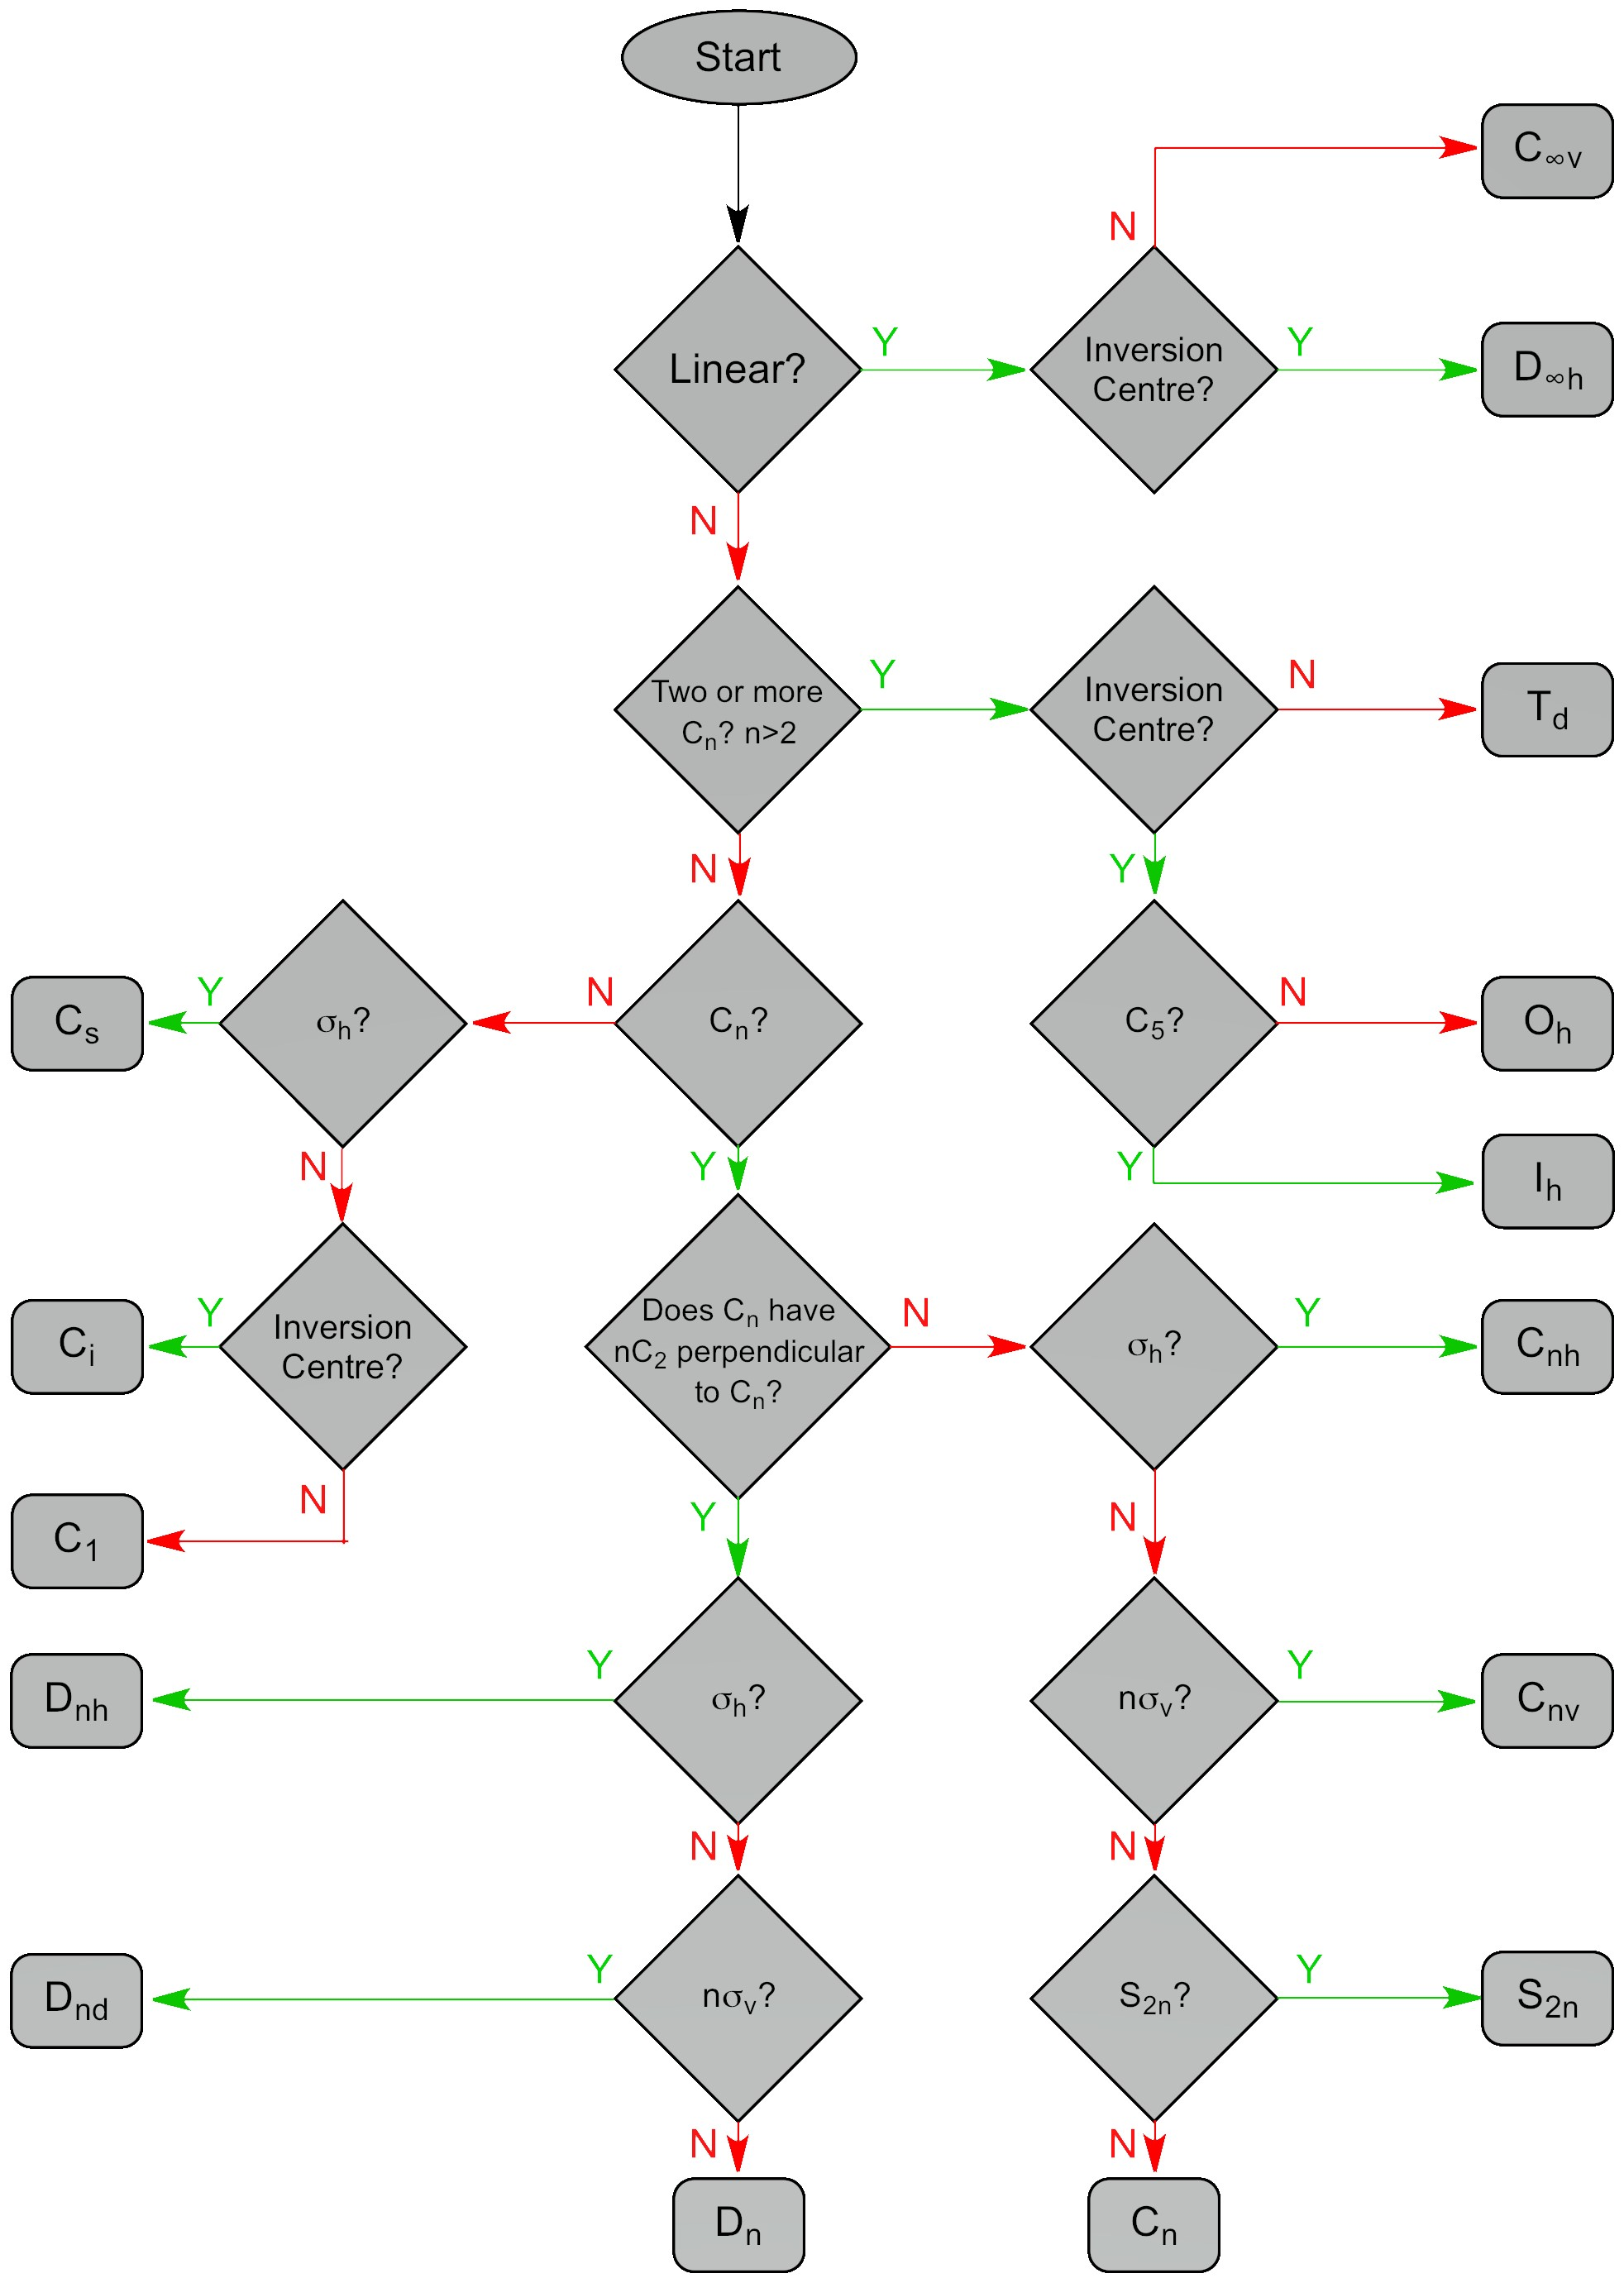
\includegraphics[width=11cm]{symflow}
	\centering
	\caption{Flowchart used to determine point groups.}
	\label{fig:symflow}
\end{figure}
Example molecules can be found in \cite{wiki_pointgroup}. 
\subsection{Representations}
\begin{defi}[Matrix representations]
A \textbf{matrix representation} is a set of \textbf{matrix representatives}, 
which presents the effect of a \textit{symmetry operation} on a molecule, 
in an \textbf{arbitrarily chosen basis}. 
\end{defi}
The choice of basis, although technically arbitrary, is usually just vectors along 
the bonds pointing from the central atom or the atomic orbitals, 
amongst other conventions for other applications. \par
For any arbitrarily chosen basis, a matrix representation can be generated. 
We can use the results from the great and little orthogonality theorems 
(see 5.10-5.11 of \cite{atkinsqm}) to \textit{reduce} a representation to 
see how many of each irreducible representation is present in the direct sum. 
Due to a theorem in group theory that states that the character (trace) of a 
representative is invariant under a change of basis (a familiarity transform), 
we can work with characters instead of matrices. 
An essential theorem on reducing representations 
(more accurately, charaters of representations) is as follows:
\begin{thrm}[Reducing representations]
The number of times an irreducible representation occurs in the reducible representation is given by
\begin{equation}
a(I)=\frac{1}{h}\sum_{\text{all classes}}\chi(R)\chi(I)N
\end{equation}
where
\begin{equation*}
\begin{aligned}
h&=\text{order of the group}\\
\chi(R)&=\text{character of the reducible representation}\\
\chi(I)&=\text{character of the irreducible representation}\\
N&=\text{number of symmetry operations in the class}
\end{aligned}
\end{equation*}
\end{thrm}
\section{Mathematical formulation}
\subsection{Notations}
See the following table for the notation we will employ: 
\begin{table}[H]
\centering
\begin{tabular}{l|l}
Meaning & Notation\\
\hline
Basis (a row vector)&$\boldsymbol{f}=(f_1,f_2,\cdots,f_d)$\\
Symmetry operations&$R,\ S,\ T,\cdots$\\
Representation of operations&$\boldsymbol{D}(R)$\\
Operation on basis&$R\boldsymbol{f}\equiv\boldsymbol{f}\boldsymbol{D}(R)$\\
Character of representation&$\chi(R)\equiv\text{tr}\bvec{D}(R)$
\end{tabular}
\caption{Notations used in group theory.}
\end{table}
\subsection{Basic theorems}
We now go on to establish some fundamental lemmas to build on later.
\begin{lemma}[Representation of group multiplication]
If $RS=T$, then $\boldsymbol{D}(R)\boldsymbol{D}(S)=\boldsymbol{D}(T)$.
\end{lemma}
\begin{proof}
\begin{equation}
\begin{aligned}
&RS\boldsymbol{f}=R[\boldsymbol{f}\boldsymbol{D}(S)]=(R\boldsymbol{f})\boldsymbol{D}(S)=\boldsymbol{f}\boldsymbol{D}(R)\boldsymbol{D}(S)=T\boldsymbol{f}=\boldsymbol{f}\boldsymbol{D}(T)\\
&\imp \boldsymbol{D}(R)\boldsymbol{D}(S)=\boldsymbol{D}(T)
\end{aligned}
\end{equation}
\end{proof}
\begin{lemma}[Representation of the inverse of operation]
The representative of the inverse of an operation is 
the inverse of the representative: 
\begin{equation}
\bvec{D}(R^{-1})=\bvec{D}(R)^{-1}. 
\end{equation}
\end{lemma}
\begin{proof}
Because we know that
\begin{equation}
RR^{-1}=E
\end{equation}
so
\begin{equation}
\bvec{D}(R)\bvec{D}(R^{-1})=\bvec{D}(E)=\bvec{I}
\end{equation}
therefore we can identify $\bvec{D}(R^{-1})$ with $\bvec{D}(R)^{-1}$.
\end{proof}
Oftentimes we would like to change the basis of a representation to simplify it, 
\ie to reduce it. We also call a change of basis a 
\textbf{similarity transformation}. An example could be the NH$_3$ molecule, where 
we originally choose a basis set of the three $s$-orbitals. But, as it will turn 
out, this is not the basis for the irreducible representation, and to find it we 
need to compute the symmetry-adapted bases of the molecule (\hl{update link}). 
Now say we have the new basis, given by 
\begin{equation*}
\begin{aligned}
s_N&=s_N\\
s_1&=s_A+s_B+s_C\\
s_2&=2s_A-s_B-s_C\\
s_3&=s_B-s_C
\end{aligned}
\end{equation*}
or, in matrix notation
\begin{equation}
\bvec{f}'\equiv\bvec{f}
\underbrace{
\begin{bmatrix}
1 &0 &0 &0\\
0 &1 &2 &0\\
0 &1 &-1& 1\\
0 &1 &-1& -1
\end{bmatrix}}_{\equiv\bvec{c}}
\end{equation}
the question is then, how to we find the representative, $\bvec{D}(R)$ in this new basis?
\begin{thrm}[Similarity transformation]
We say that two representations are \textbf{similar} if the representatives for 
the two bases are related by the \textbf{similarity transformation}:
\begin{equation}
\bvec{D}(R)=\bvec{c}\bvec{D}'(R)\bvec{c}^{-1}\ \leftrightarrow\ \bvec{D}'(R)=\bvec{c}^{-1}\bvec{D}(R)\bvec{c}.
\end{equation}
\end{thrm}
\begin{proof}
\begin{equation}
\begin{aligned}
R\bvec{f}'&=\bvec{f}'\bvec{D}'(R)\\
R\bvec{fc}&=\bvec{fcD}'(R)\\
R\bvec{f}&=\bvec{fcD}'(R)\bvec{c}^{-1}=\bvec{fD}(R)
\end{aligned}
\end{equation}
The result is immediately implied. 
\end{proof}
We introduce a lemma from linear algebra:
\begin{lemma}[Trace is invariant under cyclic permutation]
\begin{equation}
\text{tr}\bvec{ABC}=\text{tr}\bvec{BCA}=\text{tr}\bvec{CAB}.
\end{equation}
\end{lemma}
\begin{proof}
\begin{equation}
\text{tr}\bvec{ABC}=(ABC)_{ii}=A_{ik}B_{jk}C_{ki},
\end{equation}
where we have used the Einstein summation convention. Under cyclic permutation, 
the subscript continue to match, hence giving invariant trace. 
\end{proof}
\begin{thrm}[Character is invariant under similarity transform]
\label{charinv}
\begin{equation}
\chi(R)=\chi'(R).
\end{equation}
\end{thrm}
\begin{proof}
\begin{equation}
\chi(R)=\text{tr}\bvec{cD}'(R)\bvec{c}^{-1}=\text{tr}\bvec{D}'(R)=\chi'(R).
\end{equation}
\end{proof}
We need to categorise operatioons into classes, which is defined by
\begin{defi}[Classes]
Operations $R$ and $R'$ are said to be in the same class, 
or are \textit{conjugate}, if they are related as follows:
\begin{equation}
R'=S^{-1}RS, 
\end{equation}
which is to say, they are the same \textit{kind} of operation but performed 
about symmetry elements that are \textit{related by a symmetry operation}. 
\end{defi}
\begin{thrm}[Operations in the same class have the same character]
\begin{equation}
\chi(R')=\chi(R).
\end{equation}
\end{thrm}
\begin{proof}
\begin{equation}
\chi(R')=\text{tr}\bvec{D}(R')=\text{tr}\bvec{D}^{-1}(S)\bvec{D}(R)\bvec{D}(S)=\text{tr}\bvec{D}(R)=\chi(R).
\end{equation}
\end{proof}
\subsection{Irreps and orthogonality theorems}
We return to the example of NH$_3$, which belongs to the group $C_{3v}$. 
In the basis of $(s_N,s_1,s_2,s_3)$, all the representatives of 
the group operations all have two diagonal $1$'s at the top left. 
The remaining matrices are
\begin{table}[H]
\centering
\begin{tabular}{l l l}
$\bvec{D}(E)$&$\bvec{D}(C_3^+)$&$\bvec{D}(C_3^-)$\\
$
\begin{bmatrix}
1&0\\
0&1
\end{bmatrix}
$&
$\begin{bmatrix}
-1/2&-1/2\\
1/1&-1/2
\end{bmatrix}$&
$\begin{bmatrix}
-1/2&1/2\\
-1/2&-1/2
\end{bmatrix}$\\
$\bvec{D}(\sigma_v)$&$\bvec{D}(\sigma'_v)$&$\bvec{D}(\sigma''_v)$\\
$\begin{bmatrix}
1&0\\
0&-1
\end{bmatrix}$&
$\begin{bmatrix}
-1/2&1/2\\
3/2&1/2
\end{bmatrix}$&
$\begin{bmatrix}
-1/2&-1/2\\
-3/2&1/2
\end{bmatrix}$
\end{tabular}
\end{table}
We can write this as 
\begin{equation}
\bvec{D}^{(4)}=\bvec{D}^{(1)}\oplus \bvec{D}^{(1)}\oplus \bvec{D}^{(2)}
\end{equation}
All three of them are \textbf{irreducible representations} of group $C_{3v}$. 
We know that $\bvec{D}^{(2)}$ is an irreducible representation because the set 
of two by two matrices are not simultaneously diagonalisable, \ie they do not 
commute. \hl{todo: udpate link to relevant qm section}\par 
The basis for the first two $\bvec{D}^{(1)}$'s are $s_N$ and $s_1$ respectively, 
we call them
\begin{defi}[Unfaithful representation]
An \textbf{unfaithful representation} of a group is a trivial one by one matrix 
with $1$ as the sole element. 
\end{defi}
We can see that the characters for them are $(1,1,1,1,1,1)$, which means they 
belong to the $A_1$ symmetry species. The remaining irreps have characters 
$(2,-1,-1,0,0,0)$, which put them under the species $E$. $A_1$ and $E$ are also 
called $\Gamma^{(1)}$ and $\Gamma^{(3)}$ respectively. \par
Now we proceed to introduce the two very important orthogonality theorems:
\begin{thrm}[The great orthogonality theorem (GOT)]
For a group of order $h$, let $D^{(\ell)}(R)$ be the representative of the 
operation $R$ in a $d_{\ell}$-dimensional irrep of symmetry species $\Gamma^{(\ell)}$ of 
the group, then
\begin{equation}
\sum_R D_{ij}^{(\ell)}(R)^*D_{i'j'}^{(\ell')}(R)=\frac{h}{d_{\ell}}\delta_{\ell\ell'}\delta_{ii'}\delta_{jj'}.
\end{equation}
\end{thrm}
This is really a postulate at this point because we will not prove it. 
For most practical purposes though we just need the 
\begin{thrm}[The little orthogonality theorem (LOT)]
\begin{equation}
\sum_R\chi^{(\ell)}(R)^*\chi^{(\ell')}(R)=h\delta_{\ell\ell'}.
\end{equation}
\end{thrm}
\begin{proof}
We set $j=i$ and $j'=i'$, and sum over diagonal entries since we need the trace:
\begin{equation}
\begin{aligned}
\sum_{i,i'}\sum_R D_{ii}^{(\ell)}(R)^*D_{i'i'}^{(\ell')}(R)&=\sum_R\chi^{\ell}(R)^*\chi^{(\ell')}(R)\\
&=\sum_{i,i'}\frac{h}{d_{\ell}}\delta_{\ell\ell'}\delta_{ii'}\delta_{jj'}\\
&=h\delta_{\ell\ell'}, 
\end{aligned}
\end{equation}
we used the fact that the representation is of dimension $d_{\ell}$.
\end{proof}
We can simplify the theorem further by writing 
\begin{equation}
\sum_cg(c)\chi^{(\ell)}(c)^*\chi^{(\ell')}(c)=h\delta_{\ell\ell'},
\end{equation}
where $c$ is the class and $g(c)$ is the number of operations in the class. 
Setting $\ell=\ell'$ we have
\begin{equation}
\sum_cg(c)|\chi^{(\ell)}(c)|^2=h.
\end{equation}
This says that \textit{the sum of squares of the characters of any irreps of a group is equal to the order of the group}. \par
Recasting this in a vector, we can say that $\{g(c)\}^{1/2}\chi_c^{(\ell)}$ is 
a component $v_c^{(\ell)}$ of the vector $\bvec{v}^{(\ell)}$, whose components are 
distinguished by the subscript $c$. The LOT can now be written as
\begin{equation}
\bvec{v}^{(\ell)*}\cdot\bvec{v}^{(\ell')}=h\delta_{\ell\ell'}.
\end{equation}
This is saying that the two vectors are orthogonal unless $\ell'=\ell$. 
However, the number of orthogonal vectors cannot exceed the dimension of the 
space (can be far less if some of them are linearly dependent). Another analysis 
from the GOT tells that the two are actually equal. So we reach 
\begin{thrm}[Restriction 1]
The number of symmetry species is equal to the number of classes.
\end{thrm}
This analysis can be extended to GOT, with $D_{ij}^{(\ell)}(R)$ being the $R$-th 
component of a vector $\bvec{v}$ identified by three indices $\ell$, $i$ and $j$: 
\begin{equation}
\bvec{v}^{(\ell,i,j)*}\cdot\bvec{v}^{(\ell',i',j')}=\frac{h}{d_{\ell}}\delta_{\ell\ell'}\delta_{ii'}\delta_{jj'}.
\end{equation}
As the component index is $R$, we know the vectors are $h$-dimensional. Also, for 
a given $\ell$ (species/irrep), there are $d_{\ell}^2$ vectors. Therefore, 
a similar argument as the one above concludes that 
\begin{equation}
\sum_{\ell}d_{\ell}^2\leq h.
\end{equation}
We assert that the equality in fact holds, so
\begin{thrm}[Restriction 2]
\begin{equation}
\sum_{\ell}d_{\ell}^2=h.
\end{equation}
\end{thrm}
\subsection{Reducing representation}
We wish to find a suitable similarity transform that enables us to write a 
representation as a direct sum of irreps:
\begin{equation}
\bvec{D}(R)\leftrightarrow \bvec{D}'(R)=\bvec{D}^{(\Gamma^{(1)})}(R)\oplus\bvec{D}^{(\Gamma^{(2)})}(R)\oplus\cdots
\end{equation}
We introduce the notation
\begin{equation}
\Gamma=\sum_{\ell}a_{\ell}\Gamma^{(\ell)}, 
\end{equation}
where the sum is really a direct sum and multiplication is repeated direct sums 
and $a_{\ell}$ is how many times the irrep appears in the direct sum. \par
We realise that we need not necessarily find the similarity transform to find 
the coefficient $a_{\ell}$, because we can invoke \Cref{charinv}, and we can say 
\begin{equation}
\chi(R)=\chi'(R)=\sum_{\ell}a_{\ell}\chi^{(\ell)}(R).
\end{equation}
Now, determining the coefficient is within reach. Let's multiply both sides by 
$\chi^{(\ell')}(R)^*$ nad sum over all elements of the group: 
\begin{equation}
\begin{aligned}
\sum_R\chi^{(\ell')}(R)^*\chi(R)&=\sum_R\sum_{\ell}a_{\ell}\chi^{(\ell')}(R)^*\chi^{(\ell)}(R)\\
&=h\sum_{\ell}a_{\ell}\delta_{\ell\ell'}=ha_{\ell'}.
\end{aligned}
\end{equation}
Therefore
\begin{thrm}[Reduction of representations]
\begin{equation}
a_{\ell}=\frac{1}{h}\sum_{R}\chi^{(\ell)}(R)^*\chi(R).
\end{equation}
In terms of classes, 
\begin{equation}
a_{\ell}=\frac{1}{h}\sum_c g(c)\chi^{(\ell)}(c)^*\chi(c).
\end{equation}
\end{thrm}
\subsection{Symmetry-adapted bases}
After establishing the coefficients we may wish to find out what the similarity 
transformation was (which was not necessary if we just wanted to know the 
coeefficients), in other words, we can find out the basis of the new 
representation. The basis is called \textbf{symmetry-adapted basis} and the basis 
functions are called \textbf{symmetry-adapted linear combinations} (SALC). \par
We need to define
\begin{defi}[Projection operator]
The \textbf{projection operator} is defined as 
\begin{equation}
P_{ij}^{(\ell)}=\frac{d_{\ell}}{h}\sum_RD_{ij}^{(\ell)}(R)^*R.
\end{equation}
\end{defi}
\begin{prt}[Effect of the projection operator]
\begin{equation}
P_{ij}^{(\ell)}f_{j'}^{(\ell')}=f_i^{(\ell)}\delta_{\ell\ell'}\delta_{jj'}
\end{equation}
\end{prt}
\begin{proof}
Consider $\bvec{f}^{(\ell')}=(f_1^{(\ell')},f_2^{(\ell')},\cdots,f_d^{(\ell')})$ 
that form a basis for a $d_{\ell'}$-dimensional irrep $\bvec{D}^{(\ell')}$ of 
species $\Gamma^{(\ell')}$ of a group of order $h$. The effect of any operation 
of the group is 
\begin{equation}
Rf_{j'}^{(\ell')}=\sum_{i'}f_{i'}^{(\ell')}D_{i'j'}^{(\ell')}(R).
\end{equation}
Now we multiply through by an element of another representative of the same 
operation, $D_{ij}^{(\ell)}(R)$, and then sum over all elements:
\begin{equation}
\begin{aligned}
\sum_RD_{ij}^{(\ell)}(R)^*Rf_{j'}^{(\ell')}&=\sum_R\sum_{i'}D_{ij}^{(\ell)}(R)^*f_{i'}^{(\ell')}D_{i'j'}^{\ell'}(R)\\
&=\sum_{i'}f_{i'}^{(\ell')}\lf[\sum_RD_{ij}^{(\ell)}(R)^*D_{i'j'}^{(\ell')}(R)\rt]\\
&=\sum_{i'}f_{i'}^{(\ell')}\lf(\frac{h}{d_{\ell'}} \rt)\delta_{\ell\ell'}\delta_{ii'}\delta_{jj'}\\
&=\lf(\frac{h}{d_{\ell'}} \rt)\delta_{\ell\ell'}\delta_{jj'}f_i^{(\ell')}\\
&=\lf(\frac{h}{d_{\ell}} \rt)\delta_{\ell\ell'}\delta_{jj'}f_i^{(\ell)}, 
\end{aligned}
\end{equation}
where in the third equality we applied GOT and in the last equality we changed 
$\ell'$ to $\ell$ because we might as well due to the presence of 
$\delta_{\ell\ell'}$. 
\end{proof}
The reason $P$ is called the projection operator because it requires that the 
function it acts on to be the $j$-th function of the basis set of 
$\Gamma^{(\ell)}$, which then converts (projects) it to the $i$-th basis function, 
otherwise, it returns zero (orthogonal). This gives us the ability to extract all 
members of the basis set out of a single member, so long as we know the content 
of the operator. \par
A special and important case is when $\ell'=\ell$ and $i=j$, the effect of the operator is then
\begin{equation}
P_{ii}^{(\ell)}f_{j'}^{(\ell)}=f_i^{(\ell)}\delta_{ij'}.
\end{equation}
We return to this result very soon.\par
Now, if we have a set of linearly independent but otherwise arbitrary set of 
functions $\bvec{f}=(f_1,f_2,\cdots)$, which can serve as the basis of a reducible 
representation, waiting to be reduced. Just as the new basis functions can be 
expressed as linear combinations of the original basis functions, we can turn it 
around and write
\begin{equation}
f_j=\sum_{\ell',j'}f_{j'}^{(\ell')}, 
\end{equation}
where the sum is also over $\ell'$ as we're talking about the entire matrix now, 
also the coefficients are absorbed into the terms. Now let's see the effect of
\begin{equation}
P_{ii}^{(\ell)}f_j=\sum_{\ell',j'}P_ii^{(\ell)}f_{j'}^{(\ell')}=\sum_{\ell',j'}\delta_{\ell\ell'}\delta_{ij'}f_{j'}^{(\ell')}=f_i^{(\ell)}.
\end{equation}
This means that
\begin{prt}[Finding SALC]
When $P_{ii}^{(\ell)}$ operates on any member of the initial basis, it generates 
the $i$-th member of the basis for the irrep of species $\Gamma^{(\ell)}$. 
Then using $P_{ji}^{(\ell)}$ we can find the $j$-th member of the set. 
\end{prt}
However, we normally work with characters, so now we define
\begin{equation}
p^{(\ell)}\equiv\sum_iP_{ii}^{(\ell)}=\frac{d_{\ell}}{h}\sum_{i,R}D_{ii}^{(\ell)}(R)^*R=\frac{d_{\ell}}{h}\sum_R\chi^{(\ell)}(R)^*R.
\end{equation}
The effect of the operator is 
\begin{equation}
p^{(\ell)}f_j=\sum_iP_{ii}^{(\ell)}f_j=\sum_if_i^{(\ell)}.
\end{equation}
This operator thus converts any arbitrary initial basis function into a linear 
combination of the SALC.
\subsection{Decomposition of direct product bases}
\label{decompdirect}
How do we find out the symmetry species spanned by say, $xy$, if it's not reported in the character table?
The more general question is then, given that we know the symmetry species spanned by basis functions $(f_1,f_2,\dots)$, can we state the symmetry species spanned by their products, such as $(f_1^2,f_1f_2,\dots)$?
\begin{lemma}[Direct-product representation]
If $\bvec{f}^{(\ell)}$ is a basis for an irrep of $\Gamma^{(\ell)}$ of dimension $d_{\ell}$ and $\bvec{f}'^{(\ell')}$ for $\Gamma^{(\ell')}$ of dimension $d_{\ell'}$, then the products (containing mixed terms) also form the basis for a (perhaps reducible) representation, which is called a \textbf{direct product representation}, of dimension $d_{\ell}d_{\ell'}$. 
\end{lemma}
\begin{proof}
Under an operation $R$ of a group the basis functions transform as 
\begin{equation}
\begin{aligned}
&Rf_i^{(\ell)}=\sum_jf_j^{(\ell)}D_{ji}^{(\ell)}(R)\\
&Rf_{i'}^{(\ell')}=\sum_jf_{j'}^{(\ell')}D_{j'i'}^{(\ell')}(R).
\end{aligned}
\end{equation}
So their product is simply
\begin{equation}
\lf(Rf_i^{(\ell)} \rt)\lf(Rf_{i'}^{(\ell')} \rt)=\sum_{j,j'}f_j^{(\ell)}f_{j'}^{(\ell')}D_{ji}^{(\ell)}(R)D_{j'i'}^{(\ell')}(R),
\end{equation}
which is a linear combination of the products $f_j^{(\ell)}f_{j'}^{(\ell')}$.
\end{proof}
Now we have the new representation, to reduce it, we just need to work out the charater, which can be done really simply:
\begin{thrm}[Character of direct-product representation]
\begin{equation}
\chi(r)=\chi^{(\ell)}(R)\chi^{(\ell')}(R)
\end{equation}
\end{thrm}
\begin{proof}
The matrix representative of the operation $R$ in the direct-product basis is \\$D_{ji}^{(\ell)}(R)D_{j'i'}(R)$. Note especially that $jj'$ now indexes rows and $ii'$ indexes coloumns\footnote{If the two original bases contain 3 members each, the new basis now must contain 9 members, giving rise to 9x9 representatives. The rows and columns are indexed as 11, 12, 13, 21, 22 and so on.}. The diagonal elements are the elements with $j=i$ and $j'=i'$. So the character of the operation $R$ in the new basis is
\begin{equation}
\begin{aligned}
\chi(r)&=\sum_{i,i'}D_{ii}^{(\ell)}(R)D_{i'i'}^{(\ell')}(R)=\lf\{\sum_iD_{ii}^{(\ell)}(R) \rt\}\lf\{\sum_{i'}D_{i'i'}^{(\ell')}(R) \rt\}\\
&=\chi^{(\ell)}(R)\chi^{(\ell')}(R)
\end{aligned}
\end{equation}
\end{proof}
We can then reduce the characters and get the irreps. \par
But let's look at this closer: $(x,y)$ can be a basis of the $E$ irrep, and so 
$(x^2,xy,yx,y^2)$ should span $E\times E=A_1+A_2+E$. But since $xy$ and $yx$ are the same function, we should be looking at a 3-degenerate basis, so which one do we discard? We must introduce 
\begin{prt}[Symmetrised and antisymmetrised direct product]
\begin{subequations}
\begin{align}
&f_{ij}^{(+)}=\frac{1}{2}\{f_i^{(\ell)}f_j^{(\ell)}+f_j^{(\ell)}f_i^{(\ell)} \}\\
&f_{ij}^{(-)}=\frac{1}{2}\{f_i^{(\ell)}f_j^{(\ell)}-f_j^{(\ell)}f_i^{(\ell)} \}
\end{align}
\end{subequations}
The characters are given, without proof
\begin{subequations}
\begin{align}
&\chi^{+}(R)=\frac{1}{2}\lf\{\chi^{(\ell)}(R)^2+\chi^{(\ell)}(R^2) \rt\}\\
&\chi^{-}(R)=\frac{1}{2}\lf\{\chi^{(\ell)}(R)^2-\chi^{(\ell)}(R^2) \rt\}
\end{align}
\end{subequations}
\end{prt}
So it is clear that the antisymmetrised direct product for $xy$ vanishes, and the basis set $\{0,0,0\}$ has a character of $(1,1,-1)$, which is identified as $A_2$. \par
Therefore the full direct product decomposition is given as
\begin{equation}
E\otimes E=A_1\oplus[A_2]\oplus E.
\end{equation}
So $(x^2,xy,y^2)$ spans $A_1\oplus E$. Results like this will be important in working out selection rules.
\begin{prt}[Properties of direct products]
\ \par
\begin{enumerate}
	\item The direct product of anything and $A$, the \textit{totally symmetric irrep}, is itself.
	\item The direct produce of anything and itself contains the tot. sym. irrep. 
\end{enumerate}
\end{prt}
\subsection{The full rotation group}
Full rotation groups are point groups in which rotations through any angles are symmetry operations.
\paragraph{The generators of rotations}
Considering the full rotation group $R_2$ (synonymous to $C_{\inf v}$), the effect on the basis of $(x,y)$ of an infinitesimal counter-clockwise rotation by the angle $\delta\phi$ about the $z$-axis, as shown in \cref{fig:c2rot} is
\begin{equation}
\begin{aligned}
	C_{\delta\phi}(x,y)=&\{r\cos(\phi-\delta\phi),r\sin(\phi-\delta\phi) \}\\
	=&\{r\cos\phi\cos\delta\phi+r\sin\phi\sin\delta\phi,r\sin\phi\cos\delta\phi-r\cos\phi\sin\delta\phi \}
\\
	=&\{r\cos\phi+r\delta\phi\sin\phi+\dots,r\sin\phi-r\delta\phi\cos\phi+\dots \}\\
	=&(x+y\delta\phi+\dots,y-x\delta\phi+\dots)\\
	=&(x,y)-(-y,x)\delta\phi+\dots
\end{aligned}
\end{equation}
For comparison, the effect of the angular momentum operator on $(x,y)$ is
\begin{equation}
\begin{aligned}
	\hat{l}_z(x,y)=&\frac{\hbar}{i}\lf(x\diffp{}{y}-y\diffp{}{x} \rt)(x,y)\\
	=&\frac{\hbar}{i}(-y,x)
\end{aligned}
\end{equation}
so we can identify
\begin{equation}
	C_{\delta\phi}=1-\frac{i}{\hbar}\delta\phi\hat{l}_z+\dots
\end{equation}
\begin{figure}[H]
	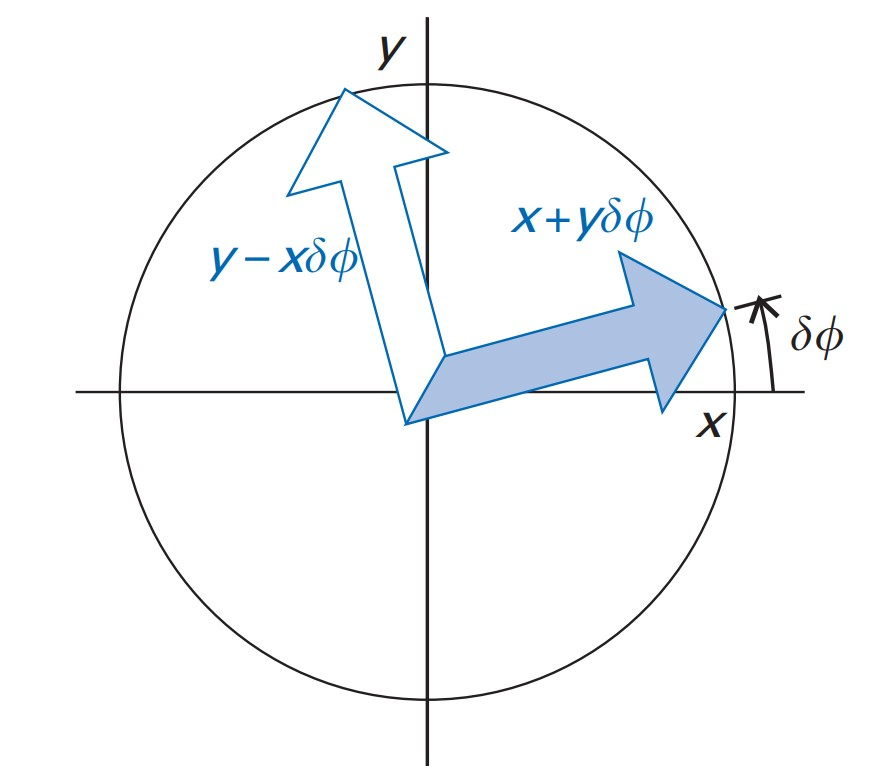
\includegraphics[width=6cm]{c2rot}
	\centering
	\caption{The effect of $C_{\delta\phi}$ on the basis of $(x,y)$.}
	\label{fig:c2rot}
\end{figure}
We have effectively expressed the classical operation $C_{\delta\phi}$ in the language of quantum mechanics, and we can call $\hat{l}_z$ the quantum mechanical generator of rotations about the $z$-axis\footnote{The classical $\hat{l}_{z,\text{class}}$ does away with the $\hbar$, \ie is just $\hat{l}_{z,\text{quant}}/\hbar$}\par
Now moving onto $R_3$, a sequential $x$ and $y$ rotation gives
\begin{equation}
\begin{aligned}
	C_{\delta\beta}^{(y)}C_{\delta\alpha}^{(x)}&=\lf(1-\frac{i}{\hbar}\delta\beta\hat{l}_y+\dots \rt)\lf(1-\frac{i}{\hbar}\delta\alpha\hat{l}_x+\dots \rt)\\
	&=1-\frac{i}{\hbar}(\delta\beta\hat{l}_y+\delta\alpha\hat{l}_x)+\lf(\frac{i}{\hbar} \rt)^2\delta\beta\delta\alpha\hat{l}_x\hat{l}_y+\dots
\end{aligned}
\end{equation}
but a sequential $y$ and $x$ rotation gives
\begin{equation}
\begin{aligned}
	C_{\delta\alpha}^{(x)}C_{\delta\beta}^{(y)}&=\lf(1-\frac{i}{\hbar}\delta\alpha\hat{l}_x+\dots \rt)\lf(1-\frac{i}{\hbar}\delta\beta\hat{l}_y+\dots \rt)\\
	&=1-\frac{i}{\hbar}(\delta\beta\hat{l}_y+\delta\alpha\hat{l}_x)+\lf(\frac{i}{\hbar} \rt)^2\delta\beta\delta\alpha\hat{l}_y\hat{l}_x+\dots
\end{aligned}
\end{equation}
so we can see that the difference between these two to the second order is 
\begin{equation}
	C_{\delta\beta}^{(y)}C_{\delta\alpha}^{(x)}-C_{\delta\alpha}^{(x)}C_{\delta\beta}^{(y)}=\lf(\frac{i}{\hbar} \rt)^2\delta\alpha\delta\beta(\hat{l}_y\hat{l}_x-\hat{l}_x\hat{l}_y)=\frac{i}{\hbar}\delta\alpha\delta\beta\hat{l}_z
\end{equation}
\begin{figure}[H]
	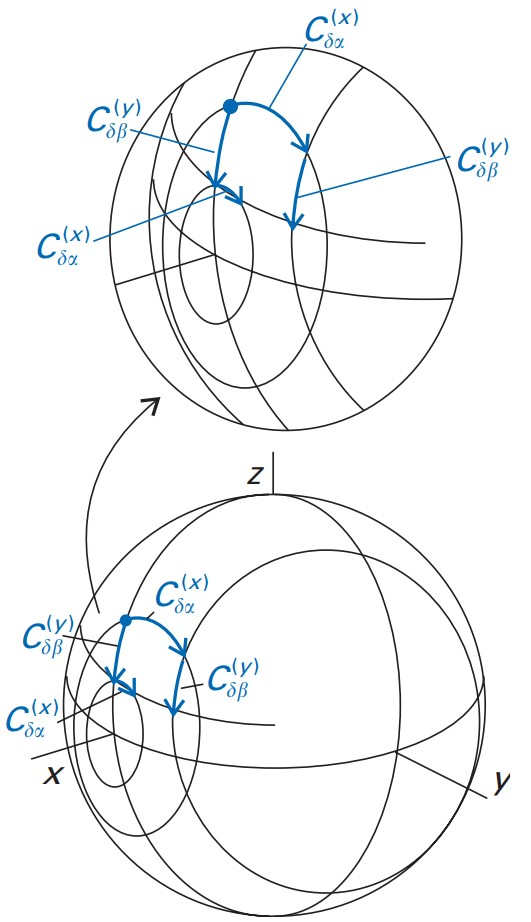
\includegraphics[width=6cm]{r3rot}
	\centering
	\caption{The difference between the two composite rotations, we can see the commutation relations graphically.}
	\label{fig:r3rot}
\end{figure}
\paragraph{The representation of the full rotation group}
The spherical harmonics $Y_{l,m_l}$ for a given $l$ transform into linear combinations of one another under a rotation, for example, the $p$-orbitals rotate into one another but not into $d$-orbitals. This is an examplification of \cref{degeneigen}, which says degenerate eigenfunctions can be related by symmetry operations.\par
Therefore, the functions $Y_{l,l},Y_{l,l-1},\dots,Y_{l,-l}$ form a basis for a $(2l+1)$-dimensional representation of the gruop. As they are orthonormal to each other, the representation is irreducible. The spherical harmonic has the form $Y_{l,m_l}=P_l^{m_l}(\cos\theta)\exp(im_l\phi) $ (\cref{sphericalharmonics}) so a rotation by $\alpha$ about the $z$-axis gives $P(\cos\theta)\exp(im_l(\phi-\alpha)) $, extending this to the entire basis we have
\begin{equation}
\begin{aligned}
	&C_{\alpha}^{(z)}(Y_{l,l},Y_{l,l-1},\dots,Y_{l,-l})\\
	=&P(\cos\theta)\lf\{\exp[il(\phi-\alpha)],\exp[i(l-1)(\phi-\alpha)],\dots,\exp[-il(\phi-\alpha)] \rt\}\\
	=&(Y_{l,l},Y_{l,l-1},\dots,Y_{l,-l})
	\begin{bmatrix}
		e^{-il\alpha} & 0 & 0 & \cdots & 0\\
		0 & e^{-i(l-1)\alpha} & 0 & \cdots & 0\\
		0 & 0 & \ddots &  & 0\\
		\vdots & \vdots &  & \ddots & \vdots \\
		0&0&\cdots&\cdots&e^{il\alpha}
	\end{bmatrix}
\end{aligned}
\end{equation}
We have identified the matrix representative of the rotation in this basis. The character of rotation is then 
\begin{equation}
\begin{aligned}
	\chi(C_{\alpha})&=e^{-il\alpha}+e^{-i(l-1)\alpha}+\dots+e^{il\alpha}\\
	&=\frac{e^{-il\alpha}[e^{i(2l+1)\alpha}-1] }{e^{i\alpha}-1}\\
	&=\frac{\sin(l+\tfrac{1}{2})\alpha}{\sin\tfrac{1}{2}\alpha}
\end{aligned}
\end{equation}
In the limit of $\alpha\rightarrow0$ (infinitesimal rotation as a symmetry operation) we get the character as $2l+1$ so we recover the fact that levels with quantum number $l$ are $(2l+1)$-fold degenerate in a spherical system.
\subsection{Group theory and angular momenta}
In the last section we saw that a quantum rigid rotor belong to the full rotation group. Now suppose there are two rotors with $j_1$ and $j_2$, belonging the irreps $\Gamma^{(j_1)}$ and $\Gamma^{(j_2)} $ with basis functions $f_{mj1}^{(j_1)} $ and $f_{mj2}^{(j_2)} $ respectively.\par
From \cref{decompdirect} we know that the bases for $\Gamma^{(j_1)}\otimes \Gamma^{(j_2)}$ are $f_{mj1}^{(j_1)}f_{mj2}^{(j_2)}$, subject to further reduction, we can write
\begin{equation}
	\Gamma^{(j_1)}\otimes \Gamma^{(j_2)}=\sum_ja_j\Gamma^{(j)}
\end{equation}
The character of rotation the system, when viewed through the decoupled picture, is 
\begin{equation}
	\chi(C_{\alpha})=\chi^{(j_1)}(C_{\alpha})\chi^{(j_2)}(C_{\alpha})=\sum_{m_{j1}=-j_1}^{j_1}\sum_{m_{j2}=-j_2}^{j_2}e^{i(m_{j1}+m_{j2})\alpha}
\end{equation}
As it contains repeated exponentials, we hope to write this in the form of
\begin{equation}
	\chi(C_{\alpha})=\sum_j\sum_{m_j}e^{im_j\alpha}
\end{equation}
which physically represents the coupled picture. To show this is possible, we realise that, purely from the mathematical form, $|m_{j1}+m_{j2}|\leq j_1+j_2$, so $|m_j|\leq j_1+j_2$ and $j\leq j_1+j_2$. Therefore $a_j=0$ for $j>j_1+j_2$. The maximum $m_j$ can only be created in one way, when $m_{j1}=j_1$ and $m_{j2}=j_2$, so $a_{j1+j2}=1$. For $m_j=j_1+j_2-1$, there are two ways to create it but one is already accounted for by the representation with $j=j_1+j_2$, so $a_{j1+j2-1}=1$, and so on. We now have the series 
\begin{equation}
	\Gamma^{(j_1)}\otimes\Gamma^{(j_2)}=\Gamma^{(j_1+j_2)}\oplus\Gamma^{(j_1+j_2-1)}\oplus\dots
\end{equation}
to terminate, we assume for a moment that $j_1>j_2$, noting that $\Gamma^{(j_i)} $ is $(2j_i+1)$-fold degenerate, so $\Gamma^{(j_1)}\otimes \Gamma^{(j_2)}$ is $(2j_1+1)(2j_2+1)$-fold degenerate, if the series terminate at $j_1-j_2$, the degeneracy on the right hand side equals the left:
\begin{equation}
\begin{aligned}
	\text{RHS}&=2[(j_1+j_2)+(j_1+j_2-1)+\dots+(j_1+j_2-2j_2)] +2j_2+1\\
	&=4j_1j_2+2j_1+2j_2+1\\
	&=\text{LHS}
\end{aligned}
\end{equation}
 This argument is exactly analogous to that given in \cref{perm_totmom}. We can write 
\begin{equation}
	\chi(C_{\alpha})=\sum_{j=|j_1-j_2|}^{j_1+j_2}\sum_{m_j=-j}^je^{im_j\alpha}=\sum_{j=|j_1-j_2|}^{j_1+j_2}\chi^{(j)}(C_{\alpha})
\end{equation}
This is essentially saying
\begin{equation}
	\Gamma^{(j_1)}\otimes\Gamma^{(j_2)}=\Gamma^{(j_1+j_2)}\oplus\Gamma^{(j_1+j_2-1)}\oplus\dots\oplus\Gamma^{(|j_1-j_2|)}
\end{equation}

\section{Applications}
\subsection{Vanishing integrals}
Consider two functions $f$ and $g$, one antisymmetric and the other symmetric 
about $x=0$. Now consider their integrals on the interval $[-a,+a]$: that of $f$ 
necessarily zero and that of $g$ can only be zero by accident. Now, if we look 
closely at the interval $[-a,+a]$ as an object, it belongs to point group $C_s$: 
identity and mirror plane. Function $f$ can be a basis of the irrep $A''$ because 
$Ef=f,\ \sigma_hf=-f$. Meanwhile, $g$ spans $A'$, the totally symmetric irrep. 
So we generalise:
\begin{lemma}[Vanishing integral]
The integral is necessarily zero if the integrand is a basis for the totally 
symmetric irreducible representation of the group. 
\end{lemma}
We now examine the products between $f$ and $g$:
\begin{enumerate}
	\item $f^2$: $A''\otimes A''=A'$, non-vanishing.
	\item $g^2$: $A'\otimes A'=A'$, non-vanishing.
	\item $fg$: $A''\otimes A'=A''$, vanishing. 
\end{enumerate}
Another way to look at this is that $f$ and $g$ are basis functions for different 
species therefore they must be orthogonal:
\begin{lemma}[Generalised vanishing integral]
If $f_i^{(\ell)}$ is the $i$-th member of a basis that spans the irrep of species 
$\Gamma^{(\ell)}$ of a group, and $f_j^{(\ell)}$ is the $j$-th member of a basis 
that spans the irrep of species $\Gamma^{(\ell)}$ of the same group, then for 
a symmetric range of integration
\begin{equation}
\int f_i^{(\ell)*}f_j^{(\ell')}\dif\tau\propto\delta_{\ell\ell'}\delta_{ij}
\end{equation}
\end{lemma}
We now are in a position to state the most important result so far
\begin{thrm}[Zero integrals]
\label{zerointegral}
An integral $\int f^{(\ell)*}f^{(\ell')}\dif\tau$ over a symmetric range is 
necessarily zero unless the integrand is a basis for the totally symmetric 
irreducible representation of the group which will be the case only if 
$\Gamma^{(\ell)}=\Gamma^{(\ell')}$. 
\end{thrm}
This can be extended to integrals of the form
\begin{equation}
I=\int f^{(\ell)*}f^{(\ell')}f^{(\ell'')}\dif\tau
\end{equation}
where the integral is necessarily zero unless the integrand is a basis for the 
totally symmetric irrep: we take $\Gamma^{(\ell)}\times\Gamma^{(\ell')}$ and 
expand out, then we take each $\Gamma^{(k)}$ in the expansion and form direct 
products $\Gamma^{(k)}\times\Gamma^{(\ell'')}$. If the tot. sym. irrep does not 
occur in the final expansion, then the integral is necessarily zero. \par
An important application of this would be determining whether a matrix element such as $H_{ij}=\lgl \psi_i |\psi_j  \rgl $ is zero. \par
In the case of the Hamiltonian, we know it is rotationally invariant \ie it belongs to the totally symmetric irrep, so all we really need to determining is whether $\psi_i$ and $\psi_j$ belong to the same irrep. \par
Another, more general example is in the case of the \emph{dipole moment operators}:\par
In a $C_{4v}$ (SF$_5$Cl say) molecule, do the integrals $\lgl d_{xy}|z |d_{x^2-y^2}  \rgl $ and $\lgl d_{xy}|l_z |d_{x^2-y^2}  \rgl $ vanish?\\
The objects span the following irreps:
\begin{center}
	\begin{tabular}{c|c}
		Object & Irrep\\
		\hline
		$d_{xy}$ & B$_2$\\
		$d_{x^2-y^2}$ & B$_1$\\
		$z$ & A$_1$\\
		$l_z$ & A$_2$
	\end{tabular}
\end{center}
Since
\begin{equation}
\begin{aligned}
&B_2\otimes A_1\otimes B_1=B_2\otimes B_1\neq A_1\\
&B_2\otimes A_2\otimes B_1=B_2\otimes B_2=A_1
\end{aligned}
\end{equation}
the former must vanish and the latter not necessarily.
\subsection{Degeneracy}
The Hamiltonian of a system must be invariant under every operation of the point 
group of the system:
\begin{equation}
RH\equiv H.
\end{equation}
A mathematical way of reasoning is that, because $H\equiv T+V$, which, take the one-dimensional harmonic oscillator for example, depends on $\diff[2]{}/{x}$ and 
$x^2$ respectively, and as such it's invariant under replacement of $x$ by $-x$, 
so the Hamiltonian spans the tot. sym. irrep of $C_s$. \par
Because $H$ is invariant under a similarity transformation of the group, \ie 
change of basis, or symmetry operation, we can write
\begin{equation}
RHR^{-1}=H.
\end{equation}
Right multiplication with $R$ gives $RH=HR$, so we can conclude that symmetry 
operations must commute with the Hamiltonian. We then introduce
\begin{thrm}[Degenerate eigenfunctions]
\label{degeneigen}
Eigenfunctions that are related by symmetry transformations of the system are degenerate, and \emph{vice versa}. 
\end{thrm}
\begin{proof}
Consider $H\psi_i=E\psi_i$. Right multiplying by $R$ gives
\begin{equation}
\begin{aligned}
RH\psi_i&=ER\psi_i\\
RH(R^{-1}R)\psi_i&=ER\psi_i\\
HR\psi_i&=ER\psi_i.
\end{aligned}
\end{equation}
Therefore, $\psi_i$ and $R\psi_i$ are degenerate.
\end{proof}
So how to determine the maximum degree of degeneracy? We recall that the 
projection operator $P_{ij}$ can give us all members of a basis set, and that it 
is formed by a linear combination of group operations, so it necessarily commutes 
with the Hamiltonian, therefore, for an irrep of dimension $d$, 
\begin{equation}
P_{ij}H\psi_j=HP_{ij}\psi_j=H\psi_i=P_{ij}E\psi_j=E\psi_i.
\end{equation}
In the same manner we can generate all $d$ members this way and they are all going 
to be degenerate, so
\begin{thrm}[Degree of degeneracy]
The degree of degeneracy of a set of functions is equal to the dimension of the 
irreducible representation they span, \ie
\begin{equation}
D=\chi(E).
\end{equation}
\end{thrm}
\subsection{Chemical bonding}
To find out which orbitals participate in bonding in a molecule, first find an appropriate basis and 
construct a reducible representation of the point group the molecule belongs to, 
and reduce it. It's that simple. We give a few examples. \par
\textbf{$\sigma$ bonding in $D_{3h}$}\\
For a choice of basis along the three bonds, we construct the character table
\begin{center}
\begin{tabular}{c|cccccc}
$D_{3h}$ & E & 2C$_3$ & 3C$_2$ & $\sigma_h$ & 2S$_3$ & 3$\sigma_v$\\
\hline
$\Gamma_1$ & $3$ & $0$ & $1$ & $3$ & $0$ & $1$
\end{tabular}
\end{center}
Reducing it with the help of $D_{3h}$ charater table, we get, for example
\begin{equation}
a(A_1')=\frac{1}{12}(3\times1+0+1\times3+3\times1+0+1\times3)=1
\end{equation}
etc., we get 
\begin{equation}
\Gamma_1=A_1'\oplus E'
\end{equation}
$A_1'$ includes $x^2+y^2$ and $z^2$, which means either the spherically symmetrical $s$ orbital or the $d_{z^2}$ orbital is involved. Same for $E'$, which either involves $p_x$ \textit{and} $p_y$ together or $d_{x^2-y^2}$ \textit{and} $d_{xy}$ together. We know the energy levels of these orbitals and therefore we can say that $s$, $p_x$ and $p_y$, \ie an $sp^2$ set, is involved in bonding.\par
\textbf{$\pi$ bonding in $D_{3h}$}\\
The basis vectors relevant for $\pi$ bonding are a set of three `out-of-plane' vectors forming the reducible representation $\Gamma_2$ and a set of three `in-plane' vectors forming $\Gamma_3$. The characters and reduction is as follows:
\begin{center}
\begin{tabular}{c|cccccc|c}
$D_{3h}$ & E & 2C$_3$ & 3C$_2$ & $\sigma_h$ & 2S$_3$ & 3$\sigma_v$ & irrep\\
\hline
$\Gamma_2$ & $3$ & $0$ & $-1$ & $-3$ & $0$ & $1$ &$A_2''\oplus E''$\\
$\Gamma_3$ & $3$ & $0$ & $-1$ & $3$ & $0$ & $-1$ &$A_2'\oplus E'$
\end{tabular}
\end{center}
Referring to the character table, we can see $\Gamma_2$ corresponds to the orbitals of $p_z,\ (d_{xz},\ d_{yz})$ together 
and $\Gamma_3$ corresponds to either $(p_x,\ p_y)$ or $(d_{x^2-y^2},\ d_{xy})$ together. \hl{what does this really mean? without a priori input how do we know to ignore the d AOs?}
\subsection{LCAOs}
Linear combinations of atomic orbital is a way to form a molecular orbital from a chosen set of basis functions. The symmetry of the LCAO must be the same as the basis functions, and that's where group theory can help us. We use the aromatic cycloproanium ion as an example.\par
\textbf{Cyclopropanium ion - $D_{3h}$}\\
We choose the $p_z$ atomic orbitals of the carbon atoms as the basis functions and since they have exactly the same directional properties as the out-of-plane vectors, the reduction is just $A_2''+E''$ again. 
So we know that the $\pi$ molecular orbitals include a doubly degenerate pair and one singly degenerate orbital. This is as far as group theory can take us. The relative energies of the orbitals can be supplied by the Huckel theory, which tells us that the energies of the orbitals are $(\alpha+2\beta),\ (\alpha-\beta),\ (\alpha-\beta)$.\par
\textbf{Cyclobutadiene - $D_{4h}$}\\
Again choosing the $p_z$ AOs, we get the reduction of $E_g+A_{2u}+B_{2u}$. The energies from Huckel theory is $(\alpha+2\beta),\ \alpha,\ \alpha,\ (\alpha-2\beta)$, and we can identify $\alpha$ with the doubly degenerate $E_g$.
\subsection{Molecular orbital correlation diagrams}
\textbf{H$_2$O}\\
The relevant orbitals are 2H $s$ and O $p$ and $s$ orbitals. 
The oxygen $p_{x/y/z}$ orbitals transform as $A_1,\ B_1,\ B_2$ respectively, 
the $s$ orbital is just $A_1$. 
The two hydrogen $s$ orbitals, \textit{together}\footnote{They must transform together since they're in a molecule, similarly, we can only identify \textit{linear combinations} of the two orbitals that transform as a component of the overall symmetry species.}, transform as $A_1\oplus B_1$. 
We can identify the linear combinations that result in the symmetry species easily as 
$(\phi_1\pm\phi_2)/\sqrt{2}$ for $A_1$ and $B_1$ respectively. \par
After identifying the symmetry species, we label them on the energy correlation diagram accordingly, but in small caps, as species for specific molecules are conventionally labelled. Only objects that belong to the same symmetry species will interact, producing a higher energy and a lower energy object, belonging to the same species. However the relative energy cannot be predicted by group theory as usual. 
\begin{figure}[H]
	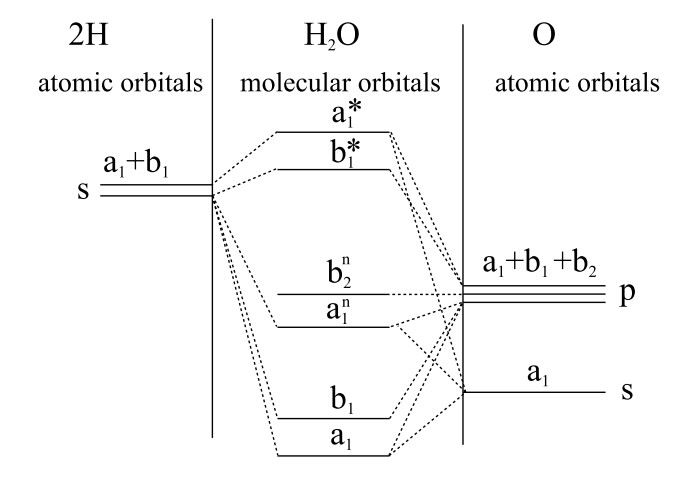
\includegraphics[width=10cm]{h2o_corr}
	\centering
	\caption{The correlation diagram for the water molecule. The two non-bonding orbitals are slightly different in energy, consistent with the photoeletron spectrum.}
	\label{fig:h2o_corr}
\end{figure}
\textbf{[Co(NH$_3$)$_6$]$^{3+}$}\\
The relevant \ie valence orbitals of cobalt are
\begin{center}
	\begin{tabular}{c|c}
	$3d$ ($x^2-y^2$ and $z^2$) & $E_g$\\
	\hline
	$3d$ ($xy,\ xz$ and $yz$) & $T_{2g}$\\
	\hline
	$4s$ & $A_{1g}$\\
	\hline
	$4p$ (all) & $T_{1u}$
	\end{tabular}
\end{center}
And now to reduce the representation formed by the L-M $\sigma$ bonds, we get $A_{1g}\oplus E_g\oplus T_{1u}$. \par
Now let the objects belonging to the same species interact, it's clear that the triply degenerate $3d\ t_{2g}$ orbitals are non-bonding since there are no matching items of the same symmetry. 
\begin{figure}[H]
	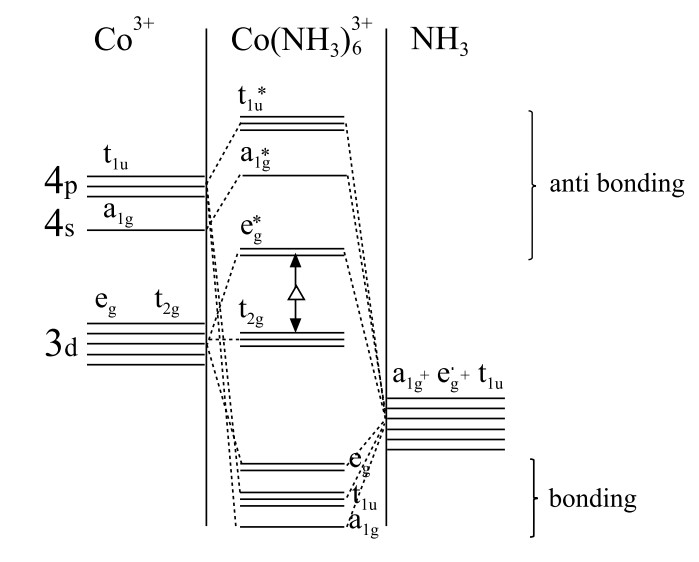
\includegraphics[width=10cm]{cobalt_corr}
	\centering
	\caption{The correlation diagram for the cobalt complex. The gap between $t_{2g}$ and $e_g^*$ is the $\Delta$ from the Ligand Field Theory.}
	\label{fig:cobalt_corr}
\end{figure}
\subsection{Molecular vibrations}
For a molecule with $N$ atoms there are $3N$ coordinates are needed to specify the spatial arrangements of the atoms. Therefore the molecule has $3N$ free variables that can be independently specified\footnote{The strict definition of degree of freedom is the number of variables needed to specify the body's configuration in \emph{phase space}, which will include the momentum \ie velocity vectors, resulting in a total of $6N$ degrees of freedom. Be clear that we're strictly talking about \emph{spatial arrangements} ($\mathbb{R}^3$) here, without considering the velocity vectors, which in this case does not matter all that much (what's knowing the speed of vibration gonna help with anything? The definition is flexible depending on the problem under consideration).}.\par
It is always true that motions of a body can be decomposed into translations, rotations and internal vibrations. For translations only the coordinates of the CoM needs to be specified, which accounts for 3 degrees of freedom, for rotations an axes need to be specified, this will take up 3 more for a non-linear molecule. For a linear molecule however the axes will not contain a component in the bond axis, therefore only 2 degrees are needed. The remaining are the number of vibrational degrees of freedom. 
\begin{thrm}[Number of possible vibrations]
For a non-linear molecule of $N$ atoms there are $3N-6$ possible vibrational modes, and $3N-5$ for a linear molecule.
\end{thrm}
The questions we will be solving is to use group theory to systematically predict the number of infrared-, and Raman-active stretches for a given molecule. The steps are given below:
\begin{enumerate}
	\item Generate a reducible representation using a basis set of 3 principal axes for every atom
	\item Reduce the representation
	\item Remove symmetry species corresponding to translations and rotations
	\item A vibration (one symmetry species, regardless of its degeneracy) is infrared active if it belongs to the same symmetry species as a component of dipole moment ($x,\ y,$ or $z$). It is Raman active if it belongs to the same symmetry species as a component of polarisability (one of the binary products or a combination of them)
\end{enumerate}
\textbf{H$_2$O}\\
The 9-vector basis reduces to $3A_1\oplus A_2\oplus 3B_1\oplus 2B_2$, from which we take out the translations $A_1,\ B_1$ and $B_2$ and rotations $A_2,\ B_1$ and $B_2$. The remaining vibrations are $2A_1\oplus B_1$, which coheres with the 3 degrees of freedom predicted by the rule of thumb. \par
The vibrations belong to symmetry species of both the dipole and polarisability, therefore water has 3 coincident infrared and Raman bands.\par
\textbf{XeF$_4$}\\
The 15-vector basis reduces to $A_{1g}\oplus A_{2g}\oplus B_{1g}\oplus B_{2g}\oplus E_g\oplus 2A_{2u}\oplus B_{2u}\oplus 3E_u $. After removal of translations and rotations we have $A_{1g}\oplus B_{1g}\oplus B_{2g}\oplus A_{2u}\oplus B_{2u}\oplus 2E_u$, a 9-degenerate representation, which coheres, as it should, with the rule of thumb. \par
Of the 9 vibrations, $A_{1g},\ B_{1g}$ and $B_{2g}$ are Raman active; $A_{2u}$ and $2E_u$ are infrared-active. $B_{2u}$ \hl{is active in neither.} Therefore there are 3 each, non-coincident infrared and Raman bands for this molecule. \par
\textbf{NH$_3$}\\
The only thing that's different is that the vectors are not pointing in the principal axes directions. 
This results a little bit of difficulty in the charaters of the rotations. 
The following results are easy to derive:
\begin{prt}[Character of $n$-fold rotation and improper rotation]
\begin{equation}
\begin{aligned}
\chi(C_n)&=1+2\cos{\frac{2\pi}{n}}\\
\chi(S_n)&=-1+\cos{\frac{2\pi}{n}}
\end{aligned}
\end{equation}
\end{prt}
\textbf{H$_3^+$}
The choice of vectors can be made such that three sets of three local axes can be transformed into one another but not mixed \ie they can be reduced separately. \hl{insert image}.
The vibrations are $A_1'+E'$, three vibrations as expected from the rule of thumb. 
\subsection{Particular vibrations}
If we only need to looks at particular vibrations, we can narrow down the choice of basis to just along the vibrations we need, instead of a general $3N$ basis. \par
For example, if we need to figure out how many carbonyl stretches will be present in a molecule, say \textbf{Ni(CO)$_4$} ($D_{4h}$), only a basis of 4 vectors are needed. It should be noted that the vector here represents extension and compression, not physical displacement from the central metal atom, so they can never be transformed into minus themselves. 
In this case the basis of 4 vectors transform as $A_{1g}\oplus B_{1g}\oplus E_u$, so we know there will be 1 infrared band and 2 Raman bands. 
In this way, geometrical isomers can be identified.\hl{fill in more examples when you have the time}\par
Another example is the ethane C-H stretches (or any X-H strecthes in other molecules). Under $D_{2h}$ group operations we get $A_g+B_{1g}+B_{2u}+B_{3u}$.
\subsection{Projection operator method}
The projection operator method can be used to determine the lienar combination of (an arbitrary set of) basis vectors that makes up a symmetry species. Applications include finding the exact vibrations in a vibrational mode, determining the LCAO, determining the functional form of HAOs, and so on. \par
The method of the projection operator is outlined as follows \hl{update and link this to the formal approach}
\begin{enumerate}
	\item Choose an arbitrary basis, reduce it
	\item Choose a `generating vector', usually something easy to work with but it's arbitrary. If degeneracy is present in any of the irreps, orthogonal generating vectors has to be chosen (\emph{e.g.} $E_g$ requires two orthogonal generating vectors whereas $T_g$ requires three)
	\item Use the \emph{extended} character table, contruct the effect of the individual operations on the generating vector
	\item Multiply all the entries with the character of the irrep, sum each row up
	\item Normalise the results
\end{enumerate}
Example: Vibrations of \textbf{BCl$_3$} ($D_{3h}$)\\
\begin{figure}[H]
	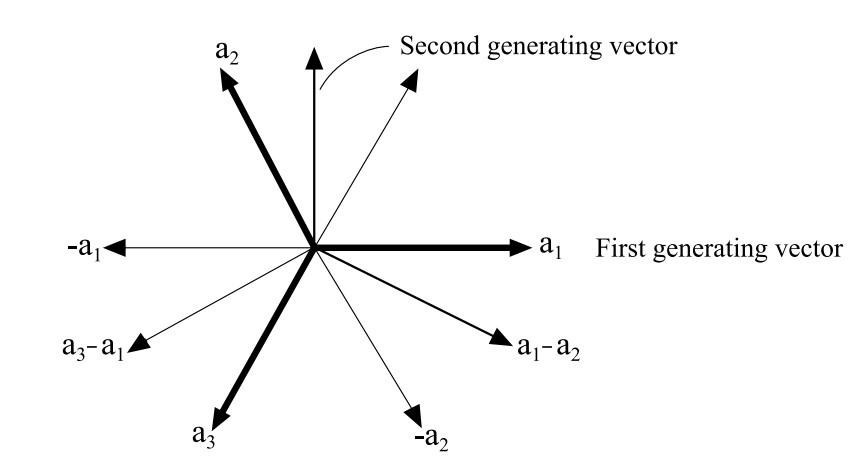
\includegraphics[width=10cm]{bcl3_vec}
	\centering
	\caption{The choice of basis and generating vectors.}
	\label{fig:bcl3_vec}
\end{figure}
\begin{figure}[H]
	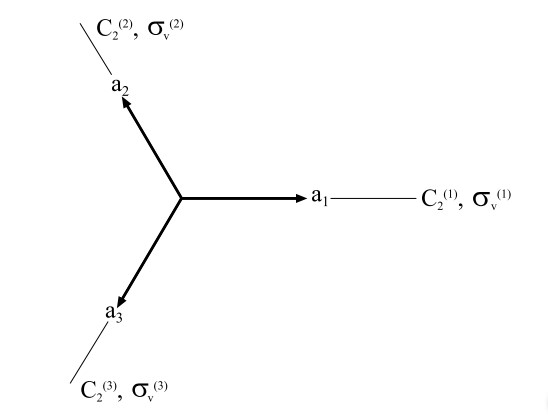
\includegraphics[width=10cm]{bcl3_sym}
	\centering
	\caption{The operations.}
	\label{fig:bcl3_sym}
\end{figure}
\textbf{Step 1:} The three-arrow basis along the bonds reduces to $A_1'+E'$.\\
\textbf{Step 2:} For the $A_1'$ mode we use $a_1$ as the generating vector, and for the $E'$ mode we use $a_1$ and one vector orthogonal to it, $a_2-a_3$\footnote{The magnitude doesn't matter.}. \\
\textbf{Step 3:} Using the extended charater table, we have
\begin{center}
	\begin{tabular}{c|cccccccccccc}
$D_{3h}$ & $E$ &$C_3$&$C_3^2$&$C_2(1)$&$C_2(2)$&$C_2(3)$&$\sigma_h$&$S_3$&$S_3^5$&$\sigma_v(1)$&$\sigma_v(2)$&$\sigma_v(3)$\\
\hline
$A_1'$ ($a_1$)&$a_1$&$a_2$&$a_3$&$a_1$&$a_3$&$a_2$&$a_1$&$a_2$&$a_3$&$a_1$&$a_3$&$a_2$ \\
$E'$ ($a_1$)&\multicolumn{5}{l}{Same as above}\\
$E'$ ($a_2-a_3$)&\dots
	\end{tabular}
\end{center}
\textbf{Step 4 and 5:} Now multiplying with the character and summing the rows, we get the normalised results
\begin{center}
	\begin{tabular}{c|c}
	Mode & Orthonormal basis\\
	\hline
	$A_1'$ & $\frac{1}{\sqrt{3}}(a_1+a_2+a_3)$\\
	$E'(x)$ & $\frac{1}{\sqrt{6}}(2a_1-a_2-a_3) $\\
	$E'(y)$ & $\frac{1}{\sqrt{2}}(a_2-a_3) $
	\end{tabular}
\end{center}
It is easy to verify that the basis is orthonormal: this means that all three bonds contribute equally as they must be due to indistinguishability. \par
The very same approach can be used to find the functional form of the HAOs of boron. We can easily identify the boron $s$ as belonging to $A_1'$, $p_x$ and $p_y$ belonging to $E'$. So we can write
\begin{center}
	\begin{tabular}{c|c}
	Orbital & Orthonormal basis\\
	\hline
	$s$ & $\frac{1}{\sqrt{3}}(a_1+a_2+a_3)$\\
	$p_x$ & $\frac{1}{\sqrt{6}}(2a_1-a_2-a_3) $\\
	$p_y$ & $\frac{1}{\sqrt{2}}(a_2-a_3) $
	\end{tabular}
\end{center}
Rearranging, we have
\begin{center}
	\begin{tabular}{c|c}
	Bond & HAO\\
	\hline
	$a_1$ & $\frac{1}{\sqrt{3}}(s+\sqrt{2}p_x)$\\
	$a_2$ & $\frac{1}{\sqrt{6}}(\sqrt{2}s-p_x+\sqrt{3}p_y) $\\
	$a_3$ & $\frac{1}{\sqrt{6}}(\sqrt{2}s-p_x-\sqrt{3}p_y) $
	\end{tabular}
\end{center}
Again it can be seen that all three orbitals contribute equally to the three HAOs.
\chapter{Solid state chemistry}
\section{Preliminary}
\subsection{Bravais lattices}
\subsubsection{Definitions}
We establish definitions below.
\begin{defi}[Bravais cystal lattice]
The \emph{Bravais cystal lattice} is one way to describe crystal lattices, as a translationally periodic array of indistinguishable mathematical points called the \emph{lattice points}. These lattice points are generated by \emph{primitive lattice vectors} (see below).
\end{defi}
\begin{defi}[Lattice motif or basis]
The lattice points are not, in general, the positions of the atoms or molecules that constitute the physical lattice, however, they are imagined to be identically attached to each of the lattice points in a \emph{motif} or \emph{basis}. The motif can be a single atom, a pair of ions (say with one on the lattic point and one a fixed translation away) and so on.
\end{defi}
\begin{defi}[Lattice vectors]
\emph{Lattice vectors} are any vectors connecting one lattice point with another.
\end{defi}
\begin{defi}[Primitive lattice vectors]
\emph{Primitive lattice vectors} can generate the whole lattice by starting at an arbitrary starting lattice point and move by integer multiples of these vectors. These define the edges of \emph{primitive unit cells}.
\end{defi}
\begin{defi}[Unit cells]
Any non-collinear lattice vectors can define the edges of a \emph{unit cell}. These are \emph{not unique}. They are said to tessellate the entire lattice.
\end{defi}
\begin{defi}[Lattice point count]
A unit cell can contain any number of lattice point. They are imagined as `pies' that are cut by the edges, or wholly contained by the cell. For example, a vertex of a cube on the lattice point will account for $\frac{1}{8}$ of a lattice point and an edge point will account for $\frac{1}{4}$ of a lattice point.
\end{defi}
\begin{defi}[Primitive unit cells]
\emph{Primitive unit cells} are unit cells that contain just one lattice point. These are also \emph{not unique}. 
\end{defi}
\subsubsection{Types of Bravais lattices}
\label{bravaistypes}
There are 14 possible Bravais lattices in three dimensions. They are classed first by their lattice systems, which contains requirements for the three lattice angles, the three cell edge lengths (not necessarily primitive lattice vector lengths unless the lattice is primitive), and the symmetry requirements.\par
Each lattice system can give rise to a maximum of 4 unit cell types:
\begin{enumerate}
	\item \textbf{Primitive} (\textbf{P}): Unit cell formed by primitive lattice vectors therefore has a lattice point at each corner.
	\item \textbf{Body-centered} (\textbf{I}): Primitive with one lattice point at the centre of the cell.
	\item \textbf{Face-centered} (\textbf{F}): Primitive with one lattice point at the centre of each face.
	\item \textbf{Base-centered} (\textbf{C}): Face-centered but with lattice points at the center of only one pair of opposing faces, which are conventionally oriented to be the base.
\end{enumerate}
We are only going to look at the cubic lattice system, which says $\alpha=\beta=\gamma=90^{\circ}$ and $a=b=c$, and requires the symmetry of at least four threefold axes at $109^{\circ}28'$ (the tetrahedral angle) to each other. The symmetry requirement excludes the base-centered unit cell type. We have three left to study in detail.
\subsubsection{The cubic lattices}
\paragraph{Simple cubic (cubic P)} 
The unit cell is just a cube with lattice points at the corners, with side length $a$, the primitive lattice vectors are 
\begin{equation*}
	\bvec{a}_1=a(1,0,0)\ \ \bvec{a}_2=a(0,1,0)\ \ \bvec{a}_3=a(0,0,1)\ \ V_c=a^3
\end{equation*}
\emph{Packing fraction}\\
Imagine spheres centered at the lattice points and they keep expanding until they just touch each other - in this case the spheres on the edges will touch first with $r=\frac{a}{2}$. This means the packing fraction, $\rho$, of primitive cubic is
\begin{equation}
	\rho=\frac{V_{\mathrm{spheres}}}{V_{\mathrm{cell}}}=\frac{\tfrac{4}{3}\pi r^3}{a^3}=\frac{\tfrac{4}{3}\pi(\tfrac{a}{2})^3}{a^3}=\frac{\pi}{6}\approx52\%
\end{equation}
\paragraph{Body-centered cubic (cubic I)} 
The unit cell that's easiest to picture and work with is a non-primitive unit cell that was described in \cref{bravaistypes}. The primitive vectors and unit cell volumes are 
\begin{equation*}
	\bvec{a}_1=\tfrac{1}{2}a(1,1,-1)\ \ \bvec{a}_2=\tfrac{1}{2}a(-1,1,1)\ \ \bvec{a}_3=\tfrac{1}{2}a(1,-1,1)\ \ V_c=\tfrac{1}{2}a^3
\end{equation*}
\emph{Packing fraction}
The spheres along the body diagonal touch first and is equal to 4 radii. The length of the body diagonal is $\sqrt{3}a=3r$, so $a=4r/\sqrt{3}$. There are 2 spheres contained in the unit cell considered, whose volume is $a^3$. The packing fraction is then given as
\begin{equation}
 	\rho=\frac{V_{\mathrm{spheres}}}{V_{\mathrm{cell}}}=\frac{2\times\tfrac{4}{3}\pi r^3}{a^3}=\frac{2\times\tfrac{4}{3}\pi r^3}{(4r/\sqrt{3})^3}=\frac{\sqrt{3}\pi}{8}\approx68\%
\end{equation} 
\paragraph{Face-centered cubic (cubic F)} 
The unit cell is again non-primitive. The primitive lattice vectors and volume of primitive unit cell are
\begin{equation}
	\bvec{a}_1=\tfrac{1}{2}a(1,1,0)\ \ \bvec{a}_2=\tfrac{1}{2}a(0,1,1)\ \ \bvec{a}_3=\tfrac{1}{2}a(1,0,1)\ \ V_c=\tfrac{1}{4}a^3
\end{equation}
\emph{Packing fraction}
In this case the spheres on the face diagonals touch first and is equal to 4 radii. The length of the face diagonal is $\sqrt{2}a$, so $a=4r/\sqrt{2}$. The unit cell contains 4 spheres. The packing fraction is therefore
\begin{equation}
	\rho=\frac{V_{\mathrm{spheres}}}{V_{\mathrm{cell}}}=\frac{4\times\tfrac{4}{3}\pi r^3}{(4r/\sqrt{2})^3}=\frac{\pi}{3\sqrt{2}}\approx74\%
\end{equation}
This is the greatest packing density possible. Therefore the cubic face-centered lattice is also known as \emph{cubic close-packed}. 
\subsubsection{Lattices with a motif}
Consider a face-centered cubic lattice, with sodium ions on the lattice points, and chloride ions $(0,0,\tfrac{1}{2}a)$ away. A pair of sodium and chloride ions forms the motif for the archetypal \ch{NaCl} lattice.
\subsection{The ionic model}
\subsubsection{The model}
Consider now a 1-D array of alternating negative and positive charges with $z_-$ and $z_+$ charges respectively, spaced $a$ apart. Starting arbitrarily from a positive charge and consider it the origin, looking to the right, the net electrostatic interaction is
\begin{equation}
	-\frac{z_+z_-e^2}{4\pi\ep_0 a}+\frac{z_+z_-e^2}{4\pi\ep_0 (2a)}-\frac{z_+z_-e^2}{4\pi\ep_0 (3a)}+\dots
\end{equation}
Now looking left as well and multiplying by the Avogadro's number we have
\begin{equation}
\begin{aligned}
	E_{\mathrm{electrostatic}}&=-2N_A\frac{z_+z_-e^2}{4\pi\ep_0 a}(1-\tfrac{1}{2}+\tfrac{1}{3}+\dots)\\
	&=-2\ln2N_A\frac{z_+z_-}{4\pi\ep_0 a}\\
	&\equiv-\mathcal{A}N_A\frac{z_+z_-e^2}{4\pi\ep_0 a}
\end{aligned}
\end{equation}
where $\mathcal{A}=2\ln2$ is the \emph{Madelung constant}, specific to each lattice under consideration.\par
However this presents the problem that the interaction energy is always attractive and predicts lattice collapse. An \emph{ansatz} repulsion term $B/a^n$ has to be introduced, corresponding to quantum mechanical repulsion between filled orbitals. The order $n$ (typically 9 or greater) is fitted \emph{post-hoc} from experimental data on equilibrium lattice spacing, and the constant $B$ can be eliminated as we will show below. The total energy as a function of lattice spacing $a$ is written as
\begin{equation}
	E(a)=-\frac{N_A\mathcal{A}z_+z_-e^2}{4\pi\ep_0a}+\frac{B}{a_n}
\end{equation}
At equilibrium, $\diff{E}/{a}=0$ and $a=a_0$, we can write
\begin{equation}
	\frac{nB}{a_0^{n+1}}=\frac{N_A\mathcal{A}z_+z_-e^2}{4\pi\ep_0a_0^2}
\end{equation}
which means we can eliminate $B$ by multiplying $a_0/n$ throughout:
\begin{equation}
	\frac{B}{a_0^n}=\frac{N_A\mathcal{A}z_+z_-e^2}{4\pi\ep_0a_0n}
\end{equation}
So the equilibrium energy is
\begin{equation}
	E_0=-\frac{N_A\mathcal{A}z_+z_-e^2}{4\pi\ep_0a_0} \lf(1-\frac{1}{n}\rt)
\end{equation}
To get an approximation for lattice energy, which involves the process of
\begin{equation*}
	\ch{MX (s) -> M+ (g) + X- (g)}
\end{equation*}
we assume that infinitely separated ions have zero energy, and so $\Delta U=-E_0$, and under such a simplistic model is it acceptable to approximate $\Delta H\approx\Delta U$, so
\begin{thrm}[Lattice energy]
The lattice energy arising from the ionic model is given as
\begin{equation}
	\Delta_L H^{\circ}\approx\frac{N_A\mathcal{A}z_+z_-e^2}{4\pi\ep_0a_0} \lf(1-\frac{1}{n}\rt)
\end{equation}
\end{thrm}
The Madelung constant for different lattices are given below
\begin{center}
	\begin{tabular}{cccc}
	\hline
	lattice & example & coordination & $\mathcal{A}$\\
	\hline
	caesium chloride & \ch{CsCl} & 8:8 & 1.763\\
	fluorite & \ch{CaF2} & 8:4 & 2.519\\
	rock salt & \ch{NaCl} & 6:6 & 1.748\\
	rutile & \ch{TiO2} & 6:3 & 2.408\\
	sphalerite & \ch{ZnS} & 4:4 & 1.638\\
	\hline
	\end{tabular}
\end{center}
\subsubsection{Radius ratios}
It is not always possible for the ions to touch if say the cations are very large, \ch{Cs+} for example and the anion is very small, \ch{F-} for example, the cations will touch first before the anions can touch the cation \emph{optimally}, meaning doing so while it still resides on the motif points. If this happens the lattice energy is not as large as it can be, and a different lattice may be adopted to allow closest approch of the ions. \par
We can work out the lowest value of $r_+/r_-$ for each lattice type:\\
\paragraph{Rock salt} 
We can work out the minimum radius ratio by drawing out the limiting scenario:
\begin{center}
	\begin{tikzpicture}
	\draw[fill=lightgray,semithick] (0,-2) circle (0.586cm);
	\draw[fill=lightgray,semithick] (2,0) circle (0.586cm);	
	\draw[semithick] (0,0) circle (1.414cm);
	\draw[semithick] (2,-2) circle (1.414cm);
	\node at (0,1) {anion};
	\node at (2,1) {cation};
	\draw[semithick] (0,0) rectangle (2,-2);
	\draw[thin,dashed] (0,0) -- (2,-2);
	\draw[<->] (-0.1,0) -- (-0.1,-2);
	\node[left] at (-0.1,-1) {$a$};
	\draw[->] (2.1,-2) -- (2.1,-0.586);
	\node[right] at (2.1, -1.293) {$r_-$};
	\draw[->] (2.7,0) -- (2.7,-0.586);
	\node[right] at (2.7,-.293) {$r_+$};
\end{tikzpicture}
\end{center}
in which the diagonal $\sqrt{2}a=2r_-$, and $a=r_-+r_+$, so we can conclude that
\begin{equation}
	\frac{r_+}{r_-}=\frac{a-\sqrt{2}a/2}{\sqrt{2}a/2}=\sqrt{2}-1\approx0.414
\end{equation}
The minimum radius ratios for other lattice types have been worked out:
\begin{center}
	\begin{tabular}{cccc}
	\hline
	lattice  & coordination & minimum radius ratio &$\mathcal{A}$\\
	\hline
	caesium chloride & 8:8 & 0.732 & 1.763\\
	rock salt & 6:6 & 0.414 & 1.748\\
	sphalerite & 4:4 & 0.225 & 1.638\\
	\hline
	\end{tabular}
\end{center}
Keeping in mind that $E\propto\mathcal{A}$, the lattice would like to keep the lattice energy as high as possible while maintaining maximum contact. For example, for \ch{MgO}, $r_+/r_-\approx0.51$, which is too small for the caesium chloride structure. So it can `choose' either rock salt of sphalerite. As rock salt has higher Madelung constant, it should be preferred, and is indeed the case.
\section{Free-electron gas model}
\subsection{Unconstrained FEG}
\subsubsection{One-dimensional FEG}
This model assumes that electrons do not interact with each other or the nuclei. Essentially they are treated as unconstrained gas molecules. In one dimension, the \sch equation was solved in \cref{freepart}, with 
\begin{equation}
	\hat{H}=-\frac{\hbar^2}{2m_e}\diff[2]{}{x}
\end{equation}
so the \sch reads
\begin{equation}
	-\frac{\hbar^2}{2m_e}\diff[2]{\psi}{x}=E\psi\ \ \imp\ \ \diff[2]{\psi}{x}=-k^2\psi
\end{equation}
where $k=\frac{2m_eE}{\hbar}$ or $E_k=\hbar^2k^2/2m_e$, the time-dependent solution is 
\begin{equation}
	|\ups_k(x,t)\rgl=Ae^{i(kx-\hbar k^2t/2m)}
\end{equation}
with momentum
\begin{equation}
	\hat{p}|\ups_k\rgl=\hbar k
\end{equation}
The wavelength can be defined as distance before the phase is reset, so in this case
\begin{equation}
	\lambda=\frac{2\pi}{|k|}
\end{equation}
\subsubsection{Three-dimensional FEG}
In three dimensions, the solution is 
\begin{equation}
	|\ups_{\bvec{k}}(\bvec{r},t)\rgl=Ae^{i\bvec{k}\cdot\bvec{r}-\hbar |\bvec{k}|^2t/2m}
\end{equation}
where
\begin{equation}
	E_{\bvec{k}}=\frac{\hbar^2|\bvec{k}|^2}{2m_e}
\end{equation}
and the momentum is
\begin{equation}
	\bvec{p}=\hbar\bvec{k}
\end{equation}
and the wavelength is
\begin{equation}
	\lambda=\frac{2\pi}{|\bvec{k}|}
\end{equation}
Now we need to introduce the important concept of 
\begin{defi}[$k$-space]
As the three-dimensional wavefunctions are defined uniquely by the wavevector $\bvec{k}$, these wavevectors can be thought to correspond to a point in the $k$-space. The squared distance from the origin is proportional to energy.
\end{defi}
\subsection{Quantization}
The unconstrained systems above are, of course, not quantised, which is a major problem. We must introduce some sort of boundary condition:
\begin{thrm}[The Born von Karman boundary conditions]
\label{fegbvk}
The BvG boundary conditions posits that the two edges of the crystals are condinuous, \ie
\begin{equation}
	\ups(\bvec{r},t)=\ups(\bvec{r}+L_i\bvec{a}_i,t)
\end{equation}
where $L_i$ is the number of cells in the $\bvec{a}_i$ direction. In effect, it requires that
\begin{equation}
	kL_1a_i=2n_1\pi\ \ \imp\ \ k=n_1\lf(\frac{2\pi}{L_1a_1} \rt)
\end{equation}
\end{thrm}
\paragraph{Justification of BvK boundary condition}
There are two ways to introduce boundary conditions:
\begin{itemize}
	\item Particle-in-a-box boundary conditions (linear wire)
	\item BvK boundary conditions (circular wire)
\end{itemize}
The table below compares the two boundary conditions
\begin{center}
	\begin{tabular}{r|l|l}
	\hline
	& Linear wire & Circular wire\\
	\hline
	Boundary conditions & $kL=n\pi$, $n\in\mathbb{Z}^+$ & $kL=2n\pi$, $n\in\mathbb{Z}$\\
	Energies & $E_n=\hbar^2\pi^2n^2/2mL^2$ & $E_n=4\hbar^2\pi^2n^2/2mL^2$\\
	Eigenfunctions & $A\sin(n\pi x/L)$ & $B\exp(2ni\pi x/L)$\\
	\hline
	\end{tabular}
\end{center}
Basically, the energy levels for the two models look like this
\begin{center}
	\begin{tikzpicture}[scale=0.3]
	\node at (-2,19){\textbf{Linear wire}};
	\node at (7,19){\textbf{Circular wire}};
	\draw[->] (-10,-2) -- (-10,18) node [anchor=east] {$E_n$};
	\draw (0,1)node[anchor=east] {$n=1,E_n=1$} -- (1,1);
	\draw (0,4)node[anchor=east] {$n=2,E_n=4$} -- (1,4);
	\draw (0,9)node[anchor=east] {$n=3,E_n=9$} -- (1,9);
	\draw (0,16)node[anchor=east] {$n=4,E_n=16$} -- (1,16);
	\draw (4,-1) -- (5,-1)node[anchor=west]{$n=0,E_n=0$};
	\draw (4,4) -- (5,4);
	\draw (5.25,4) -- (6.25,4)node[anchor=west]{$n=\pm1,E_n=4$};
	\draw (4,16) -- (5,16);
	\draw (5.25,16) -- (6.25,16)node[anchor=west]{$n=\pm2,E_n=16$};
\end{tikzpicture}
\end{center}
And in the limit that $N\rightarrow\inf$, the density of states is approximately the same, and also the HOMO, now Fermi level, is also the same.\par
So what's different? The reason for choosing the circular wire is threefold:
\begin{enumerate}
	\item The eigenfunctions of the linear wire are not eigenfunctions of the momentum operator, while the circular wire ones are, yielding $\hbar\bvec{k}$ naturally.
	\item By ignoring the surface effects, the boundary conditions of the linear wire do not arise as there's no `outside' where $V(x)=\inf$.
	\item The circular wire allows potential energy functions of symmetry $V(x+N\bvec{a})=V(x)$, while the linear wire does not. This is important in the full theory.
\end{enumerate}
Simply put, the crystal is imagined to be infinite so that the edge effects are ignored. \par
In the $k$-space, the allowed wavefunctions (states) are just a series of points spaced $2\pi/L_1a_1$ apart. The density of BvK allowed states in 1D is therefore
\begin{equation}
	\frac{L_1a_1}{2\pi}\equiv\frac{\mathcal{L}}{2\pi}
\end{equation}
where $\mathcal{L}=L_1a_1$ is called the BvK length.\par
In two and three dimensions the density of BvK allowed states are readily generalised to
\begin{equation}
\begin{aligned}
&\text{2D: }\frac{L_1L_2A_c}{(2\pi)^2}\equiv\frac{\mathcal{A}}{(2\pi)^2}\\
&\text{3D: }\frac{L_1L_2L_3V_c}{(2\pi)^2}\equiv\frac{\mathcal{V}}{(2\pi)^3}
\end{aligned}
\end{equation}
\subsection{Fermi-Dirac distribution}
The Maxwell-Boltzmann distribution assumes that the particles are distinguishable and any number of particles can occupy a level. However that is clearly not applicable to electrons, which are fermions. The Pauli exclusion principle states that two of more \emph{identical fermions} cannot occupy the same quantum state. A distribution adhering to the Pauli exclusion principle is the 
\begin{thrm}[Fermi-Dirac distribution]
The distribution states that the average number of fermions in a single-particle state $i$ is given by
\begin{equation}
	\lgl n_i\rgl=\frac{1}{\exp[(\ep_i-\mu)/kT]+1}
\end{equation}
where we can write $\lgl n_i\rgl$ as $f(\ep_i)$, and approximate the chemical potential $\mu$ with the \emph{Fermi energy}, $\ep_{\mathrm{F}}$, to give
\begin{equation}
	f(\ep_i)=\frac{1}{\exp[(\ep_i-\ep_{\mathrm{F}})/kT]+1}
\end{equation}
\end{thrm}
\begin{figure}[ht]
	\centering
	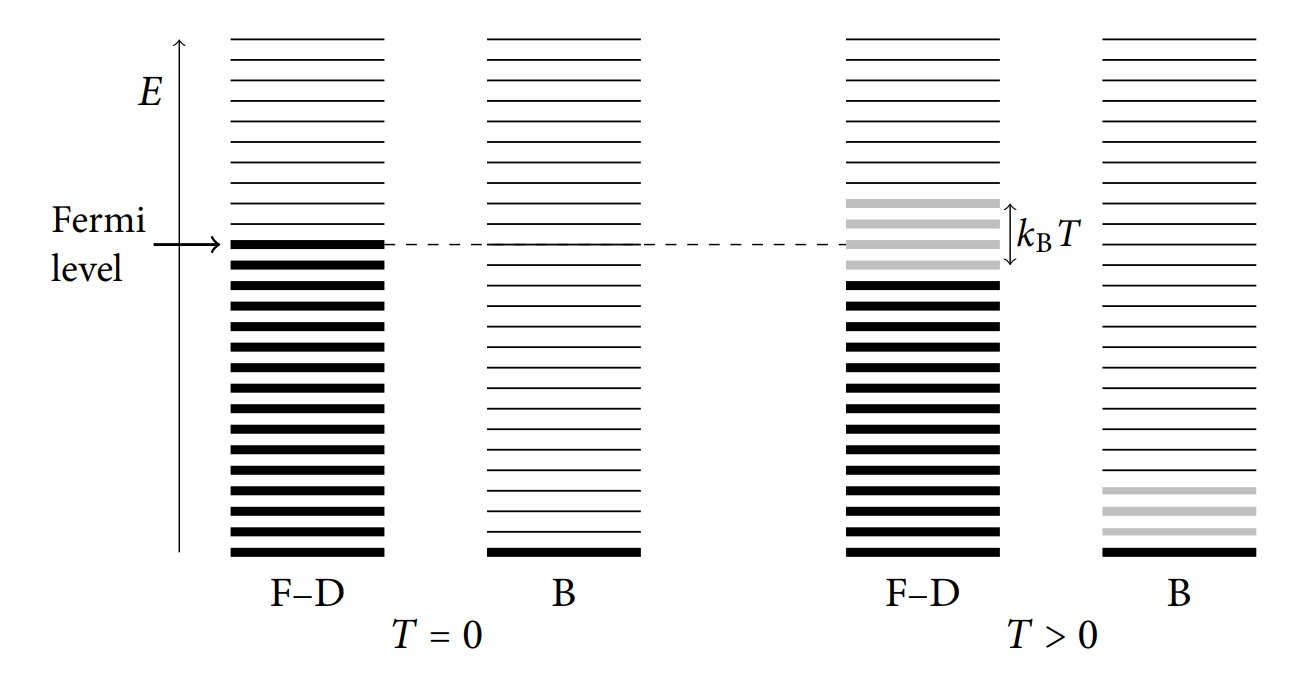
\includegraphics[width=8cm]{fermilevels}
	\caption{Comparison between the predictions of Fermi-Dirac and Maxwell-Boltzmann distributions}
	\label{fig:fermilevels}
\end{figure}
The result is a logistic function ranging from 1 for energies much lower than the Fermi level to 0 for energies much higher than the Fermi level. Raising the temperature has the effect of exciting particles near the Fermi level, `blurring' the distribution:
\begin{figure}[ht]
	\centering
	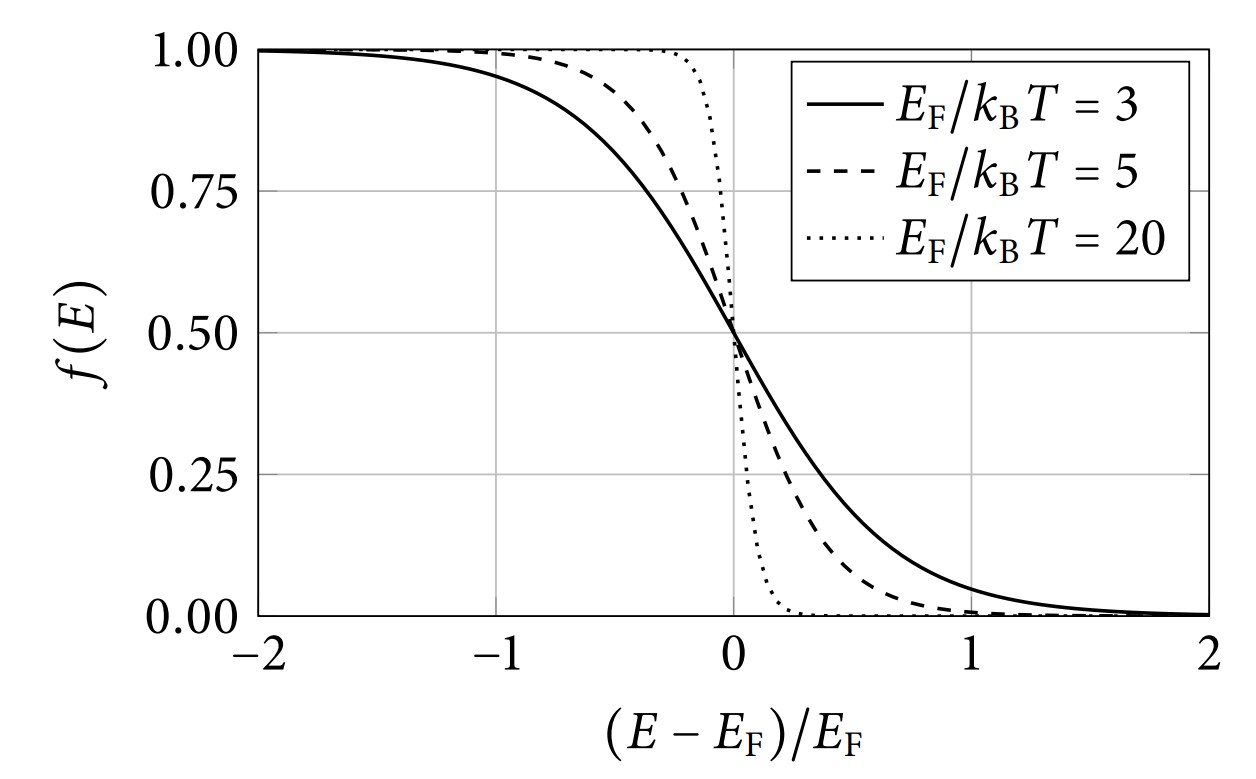
\includegraphics[width=8cm]{fermigraph}
	\caption{The blurring of the Fermi-Dirac distribution occurs at higher temperautres. Notice it always runs from 1 to 0, as required by the Pauli exclusion principle.}
	\label{fig:fermigraph}
\end{figure}
\begin{defi}[Fermi quantities]
The \emph{Fermi energy} is defined only at 0 K, which is defined as the highest filled level at 0K.\par
The \emph{Fermi level}, $E_{\mathrm{F}}$ is the energy level correponding to Fermi energy, but remains defined for all temperatures.\par
The \emph{Fermi wavevector}, $\bvec{k}_{\mathrm{F}}$ is the wavevector corresponding to the Fermi level.\par
Alternatively, the Fermi level can be approximately seen to be the energy level that has half occupancy at non-zero temperatures.
\end{defi}
\subsection{Properties of the FEG}
\subsubsection{Density of states}
The density of BvK states in 3D is 
\begin{equation}
	W(E)=\underbrace{\vphantom{\frac{\mathcal{V}}{(2\pi)^3}} \frac{4}{3}\pi|\bvec{k}|^3}_{\mathrm{`volume'}}\times\underbrace{\frac{\mathcal{V}}{(2\pi)^3}}_{\mathrm{density}}
\end{equation}
and we know that
\begin{equation}
	|\bvec{k}|=\lf(\frac{2m_eE}{\hbar^2} \rt)^{\frac{1}{2} }
\end{equation}
Keeping in mind that we although each level can accept only one \emph{identical} Fermion, electrons have two spin states and they spin-pair so each level can be doubly occupied, so a factor of two is applied in front:
\begin{equation}
	W(E)=2\times\frac{4}{3}\pi|\bvec{k}|^3\times\frac{\mathcal{V}}{(2\pi)^3}=\frac{|\bvec{k}|^3\mathcal{V}}{3\pi^2}=\frac{\mathcal{V}}{3\pi^2}\lf(\frac{2m_eE}{\hbar^2} \rt)^{\frac{3}{2}}
\end{equation}
Density of states soon follows by simple differentiation
\begin{thrm}[Density of BvK states]
The number of BvK states with energy up to $E$ is given as
\begin{equation}
	W(E)=\frac{\mathcal{V}}{3\pi^2}\lf(\frac{2m_eE}{\hbar^2} \rt)^{\frac{3}{2}}
\end{equation}
so the density of states is given as
\begin{equation}
	D(E)=\diff{W(E)}{E}=\frac{\mathcal{V}}{2\pi^2}\lf(\frac{2m_e}{\hbar^2} \rt)^{\frac{3}{2}}E^{\frac{1}{2}}
\end{equation}
We note that the density of states increase with energy.
\end{thrm}
\subsubsection{Fermi quantities}
Suppose that the number density of electrons in the metal is $n_e$, so there are $n_e\mathcal{V}$ electrons in the BvK volume. At absolute zero, where Fermi energy is defined, we can say that the number of states filled are equal to the number of electrons\footnote{Although we commonly think of the levels as being doubly filled, for the formalism of the BvK we think of two degenerate levels at the same energy, one for the spin up electron one for the spin down.}, which is to say
\begin{equation}
	W(E_{\mathrm{F}})=n_e\mathcal{V}
\end{equation}
so
\begin{equation}
\begin{aligned}
	&\frac{\mathcal{V}}{3\pi^2}\lf(\frac{2m_eE_{\mathrm{F}}}{\hbar^2} \rt)^{\frac{3}{2}}=n_e\mathcal{V}\\
	\imp&E_{\mathrm{F}}=\lf(\frac{\hbar^2}{2m_e} \rt)(3\pi^2n_e)^{3/2}
\end{aligned}
\end{equation}
And the Fermi wavevector can also be worked out:
\begin{equation}
	|\bvec{k}|_{\mathrm{F}}=(3\pi^2n_e)^{1/3}
\end{equation}
To summarise
\begin{thrm}[Fermi level and wavevector]
For a metal with eletron density $n_e$, the Fermi level and Fermi wavevector are given as
\begin{equation}
\begin{aligned}
&E_{\mathrm{F}}=\lf(\frac{\hbar^2}{2m_e} \rt)(3\pi^2n_e)^{3/2}\\
&|\bvec{k}|_{\mathrm{F}}=(3\pi^2n_e)^{1/3}
\end{aligned}
\end{equation}
\end{thrm}
\subsubsection{Average energy}
At absolute zero the average energy is
\begin{equation}
	\lgl E\rgl=\frac{\text{total energy}}{\text{number of states}}=\frac{\int^{E_\text{F}}_0E\times D(E)\dif E}{\int^{E_\text{F}}_0D(E)\dif E}
\end{equation}
The integrals are straightforward and the result is 
\begin{thrm}[Average energy at absolute zero]
The Fermi-Dirac distribution predicts that for a free electron gas, the average energy at absolute zero is
\begin{equation}
	\lgl E\rgl=\frac{3}{5}E_{\mathrm{F}}
\end{equation}
\end{thrm}
\subsubsection{Heat capacity}
Assuming that the metal atom has only 1 valence electron, one mole of the metal contains $N_A$ valence electrons. To a crude approximation, the number of excited electrons (those within $kT$ of Fermi level) is
\begin{equation}
	n=N_A\times\frac{kT}{E_{\mathrm{F}}}=\frac{RT}{E_{\mathrm{F}}}
\end{equation}
Again, to an approximation, these electrons on average has $kT$ more in energy\footnote{They already had some intrinsic kinetic energy as a consequence of the Fermi-Dirac distribution, and now they have an additional $kT$ in `thermal' energy, which is just additional kinetic energy.}, so the total increase in energy as a result of raised temperature is
\begin{equation}
	\Delta U=kT\frac{RT}{E_{\mathrm{F}}}\equiv\frac{R}{T_{\mathrm{F}}}T^2
\end{equation}
where $T_{\mathrm{F}}=E_{\mathrm{F}}/k$ is the \emph{Fermi temperature}, so the heat capacity is roughly
\begin{equation}
	C_{V,m}=\frac{2R}{T_{\mathrm{F}}}\times T
\end{equation}
This treatment gives poor agreement with data, as the estimation of the number of electrons is poor and does not take into account the density of states. A more sophisticated treatment gives
\begin{equation}
	C_{V,m}=\frac{\pi^2RT}{2T_{\mathrm{F}}}
\end{equation}
\subsubsection{Bulk modulus}
The bulk modulus is the ratio between the pressure change and the fractional change in volume, which, in calculus terms is
\begin{equation}
	B=-V\diffp pV[T,N]
\end{equation}
Also the definition of pressure in terms of the internal energy is
\begin{equation}
	p=-\diffp UV[N]
\end{equation}
At absolute zero, we know the average energy, so the internal energy is
\begin{equation}
	U=N\lgl E\rgl=\frac{3}{5}NE_{\mathrm{F}}
\end{equation}
The Fermi energy is
\begin{equation}
	E_{\mathrm{F}}=\lf(\frac{\hbar^2}{2m_e} \rt)(3\pi^2n_e)^{2/3}
\end{equation}
The electron number density, in the formalism of BvK is just 
\begin{equation}
	n_e=\frac{N}{\mathcal{V}}
\end{equation}
So we can write 
\begin{equation}
	U=\frac{3}{5}N\underbrace{\lf(\frac{\hbar^2}{2m_e} \rt)(3\pi^2N)^{2/3}}_{c}\mathcal{V}^{-2/3}
\end{equation}
So 
\begin{equation}
	p=\frac{2}{5}Nc\mathcal{V}^{-5/3}
\end{equation}
and the bulk modulus is
\begin{equation}
	B=\frac{2}{3}Nc\mathcal{V}^{-5/3}
\end{equation}
Since $E_{\mathrm{F}}=c\mathcal{V}^{-2/3}$, we can finally write
\begin{equation}
	B=\frac{2}{3}E_{\mathrm{F}}N/\mathcal{V}=\frac{2}{3}E_{\mathrm{F}}n_e
\end{equation}
\subsubsection{Electrical conductivity}
The `ground state' of a 2-dimensional FEG in the $k$-space at 0 K will show occupied $k$-states within a circle of radius $|\bvec{k}|$ centred at $(0,0)$, as the highest occupied level is the Fermi level (at 0 K), and the momentum given by $\hbar\bvec{k}$ is on average zero. The circle is called the \emph{Fermi circle}.\par
Now after the application of an electric field along the $x$-direction, the average momentum will be in the $x$-direction\footnote{It is not infinite because electrons are scattered so a steady-state \emph{drift velocity} is reached.}, so the centre of the Fermi circle will be shifted to the right.\par
It is important to note that the only reason conduction can happen is because there are vacant states just outside the Fermi circle.\par
A simple model that can give us the conductivity is the
\begin{thrm}[The Drude model]
The Drude model says that the drift velocity, $v_{\mathrm{d}}$ is given by
\begin{equation}
	v_{\mathrm{d}}=e\mathcal{E}\tau/m_{\mathrm{e}}
\end{equation}
\end{thrm}
\begin{proof}
	The net acceleration experienced by the electron due to the field is $e\mathcal{E}/m_{\mathrm{e}}$. Supposing that the average time between collisions is $\tau$, which knocks the speed down to zero again, the average velocity is just accleration times time, which gives the result required.
\end{proof}
The current density is defined as the charge per unit time per unit area, which can be written as
\begin{equation}
	j=\frac{n_{\mathrm{e}}v_{\mathrm{d}}\Delta tAe}{\Delta tA}=n_{\mathrm{e}}v_{\mathrm{d}}e=n_{\mathrm{e}}e^2\mathcal{E}\tau/m_{\mathrm{e}}
\end{equation}
The Ohm's law says that 
\begin{equation}
	j=\sigma\mathcal{E}
\end{equation}
so we can extract
\begin{equation}
	\sigma=n_{\mathrm{e}}e^2\tau/m_{\mathrm{e}}
\end{equation}
The \emph{electron mobility}, $\mu_{\mathrm{e}}$ (not magnetic susceptibility) is 
\begin{equation}
	\mu_{\mathrm{e}}\equiv\frac{v_{\mathrm{d}}}{\mathcal{E}}=\frac{e\tau}{m_{\mathrm{e}}}
\end{equation}
\subsection{The nearly-free electron gas}
\subsubsection{Failure of the FEG and Brillouin zones}
The free electron gas assumes no interactions whatsoever with the underlying lattice, which is of course not true. The FEG model notably fails when the wavefunctions $\psi_{\bvec{k}}$ are diffracted by the lattice. To take this into account, the Brillouin zone is defined:
\begin{defi}[Brillouin zone]
The boundaries of the \emph{Brillouin zone} in $k$-space are collections of wavefunctions that undergo Bragg diffraction\footnote{This means the waves are refracted by atoms on a series of parallel planes in the \emph{real space}.}. These boundaries are therefore also called Bragg planes. The first Brillouin zone correspond to the collection of $k$-states reachable from the origin without having to cross a Bragg plane, while the second Brillouin zone are such points reachable by crossing just one Bragg plane, and so on.
\end{defi}
We need to find the Bragg planes in $k$-space now. Referring to \hl{draw diagram}, we can see that the Bragg condition is
\begin{equation}
	2a\sin\theta=n\lambda
\end{equation}
where $n$ is the integer and will be the order of the Brillouin zone. The de Broglie relation of the incoming waves says
\begin{equation}
	\lambda=\frac{h}{|\bvec{p}|}=\frac{h}{\hbar|\bvec{k}|}=\frac{2\pi}{|\bvec{k}|}
\end{equation}
So we now have
\begin{equation}
	2a\sin\theta=\frac{2\pi n}{|\bvec{k} |}
\end{equation}
Realising that $|\bvec{k}|\sin\theta$ is the component of the wavevector perpendicular to the diffracting plane\footnote{Remember that $\bvec{p}=\hbar\bvec{k}$, so the wavevector just lies in the direction of propagation / incidence.}, we can just write
\begin{equation}
	k_{\perp}=\frac{n\pi}{a}
\end{equation}
In one dimension, as $|\bvec{k}|=k_{\perp}$, the Bragg planes are just scalar points at integer multiples of $n\pi/a$. In two dimensions, the constrcution method is to draw perpendicular bisectors connecting the origin and the closest four points in the \emph{reciprocal lattice}, which will enclose the first Brillouin zone, and then the same is repeated for the next four closest points, for the second Brillouin zone and so on, always extend the Bragg planes as long as possible so you don't get confused whether you've crossed a Bragg plane or not.
\begin{center}
	\begin{tikzpicture}
	\draw[thick,fill=purple!60!white] (-1,-0.5) rectangle (1,0.5);
	\draw[thick,fill=purple!60!white] (-0.5,-1) rectangle (0.5,1);		
	\draw[thick,fill=yellow!60!white] (-1,0)--(0,1)--(1,0)--(0,-1)--(-1,0);	
	\draw[thick,fill=green!60!white] (-0.5,-0.5) rectangle (0.5,0.5);

	\foreach \x in {-3,-2,...,3}{
		\foreach \y in {-3,-2,...,3}{
			\node[draw,circle,inner sep=1pt,fill] at (\x,\y){};
		}
	}
	\node[left] at (0,0){$\Gamma$};
	\draw[-{Stealth},thick](0,0)--(0,1) node[above]{1};
	\draw[-{Stealth},thick](0,0)--(1,1) node[right]{2};
	\draw[-{Stealth},thick](0,0)--(2,0) node[above]{3};
	\draw[-{Stealth},thick](0,0)--(2,-1) node[below]{4};

	\draw[dashed](-3,0.5)--(3,0.5);
	\draw[dashed](-3,-0.5)--(3,-0.5);
	\draw[dashed](0.5,-3)--(0.5,3);
	\draw[dashed](-0.5,-3)--(-0.5,3);

	\draw[dashed](-2,3)--(3,-2);
	\draw[dashed](2,3)--(-3,-2);
	\draw[dashed](-2,-3)--(3,2);
	\draw[dashed](2,-3)--(-3,2);

	\draw[dashed](1,3)--(1,-3);
	\draw[dashed](-1,3)--(-1,-3);
	\draw[dashed](-3,1)--(3,1);
	\draw[dashed](-3,-1)--(3,-1);

	\draw[dashed](0,2.5)--(2.5,-2.5);
	\draw[dashed](-2.5,2.5)--(0,-2.5);
	\draw[dashed](0,-2.5)--(2.5,2.5);
	\draw[dashed](-2.5,-2.5)--(0,2.5);
	\draw[dashed](-2.5,0)--(2.5,-2.5);
	\draw[dashed](-2.5,2.5)--(2.5,0);
	\draw[dashed](-2.5,0)--(2.5,2.5);
	\draw[dashed](-2.5,-2.5)--(2.5,0);
\end{tikzpicture}
\end{center}
Note that the fourth Brillouin zone is not coloured in.
\subsubsection{Reciprocal lattice}
The motivation for defining a reciprocal lattice is to construct a lattice in $k$-space with a periodicity that's related to the real space lattice. The simplest way to fulfil that is to consider a collection of waves in real space such that
\begin{equation}
	\ups_{\bvec{k}}(\bvec{r})=\ups_{\bvec{k}}(\bvec{r}+\bvec{R})
\end{equation}
where $\bvec{R}$ is any lattice vector (not just primitive vectors). Essentially, their phase differ by some integer multiple between $2\pi$ between lattice points. A collection of these waves in $k$-space forms the reciprocal lattice. The equation above can be further developed:
\begin{equation}
\begin{aligned}
	&\ups_0e^{i\bvec{k}\cdot\bvec{r}}=\ups_0e^{i\bvec{k}\cdot(\bvec{r}+\bvec{R})}\\
	\imp& e^{i\bvec{k}\cdot\bvec{R}}=1\\
	\imp& \bvec{k}\cdot\bvec{R}=2n\pi
\end{aligned}
\end{equation}
Considering that $\bvec{R}=\sum A_i\bvec{a}_i$ and $\bvec{k}=\sum B_i\bvec{b}_i$, we can choose the simplest basis\footnote{The matrix equation is 
\begin{equation}
	\begin{pmatrix}
		B_1&B_2&B_3
	\end{pmatrix}
	\begin{pmatrix}
		\bvec{b}_1\cdot\bvec{a}_1 & \bvec{b}_1\cdot\bvec{a}_2 & \bvec{b}_1\cdot\bvec{a}_3\\
		\bvec{b}_2\cdot\bvec{a}_1 & \bvec{b}_2\cdot\bvec{a}_2 & \bvec{b}_2\cdot\bvec{a}_3\\
		\bvec{b}_3\cdot\bvec{a}_1 & \bvec{b}_3\cdot\bvec{a}_2 & \bvec{b}_3\cdot\bvec{a}_3		
	\end{pmatrix}
	\begin{pmatrix}
		A_1\\
		A_2\\
		A_3
	\end{pmatrix}=2n\pi
\end{equation}
so there can be more than one way to choose the basis set $\{\bvec{b}_i\}$, but obviously the easiest way out is to make it orthogonal to $\{\bvec{a}_i\}$. The remaining coefficients must have $\sum A_iB_i=n$, since the $A_i$'s are integers and $l$ is a integer, the $B_i$'s have to be integers as well, \ie the $\bvec{b}_i$'s are primitive vectors for the reciprocal lattice.
}
so that
\begin{equation}
	\bvec{b}_i\cdot\bvec{a}_j=\delta_{ij}
\end{equation}
This way we can construct a reciprocal lattice from a real lattice. The above relation is general and easily applied in 2D cases, however in 3D the following relation, derive from the expression above, can come in handy:
\begin{equation}
	\bvec{b}_3=\frac{2\pi(\bvec{a}_1\times\bvec{a}_2)}{\bvec{a}_3\cdot(\bvec{a}_1\times\bvec{a}_2)}
\end{equation}
and cyclic permutations thereof.\par 
The derivation is simple once we note that 
\begin{equation}
	\frac{(\bvec{a}_1\times\bvec{a}_2)}{\bvec{a}_3\cdot(\bvec{a}_1\times\bvec{a}_2)}=\frac{\bvec{a}_3}{|\bvec{a}_3|}
\end{equation}
We also note that $\bvec{a}_3\cdot(\bvec{a}_1\times\bvec{a}_2)=V_{\mathrm{c}}$, the volume of unit cell. 
The foregoing is summarised below
\begin{thrm}[Construction of reciprocal lattice]
The reciprocal lattice primitive vectors are given, in general
\begin{equation}
	\bvec{b}_i\cdot\bvec{a}_j=\delta_{ij}
\end{equation}
and in 3D, 
\begin{equation}
	\bvec{b}_3=\frac{2\pi(\bvec{a}_1\times\bvec{a}_2)}{V_{\mathrm{c}}}
\end{equation}
and cyclic permutations thereof.
\end{thrm}
The volume of the reciprocal lattice unit cell is 
\begin{equation}
	\Omega=\bvec{b}_1\cdot(\bvec{b}_2\times\bvec{b}_3)
\end{equation}
which is 
\begin{equation}
	\Omega=\frac{(2\pi)^2}{V_{\mathrm{c}}^3}(\bvec{a}_1\times\bvec{a}_2)\cdot[(\bvec{a}_2\times\bvec{a}_3)\times(\bvec{a}_3\times\bvec{a}_1)]
\end{equation}
the big vectorial mess at the end is a number since overall it's a dot product, and since it involves every vector twice, it's just $V_{\mathrm{c}}^2$, so the reciprocal unit cell volume is 
\begin{equation}
	\Omega=\frac{(2\pi)^3}{V_{\mathrm{c}}}
\end{equation}
\subsubsection{Boundary cases}
The foregoing discussion pointed out the FEG approximations fail at Bragg planes, which is to say the dispersion curve have \emph{discontinuities} at Bragg planes. This provides a motivation for us to study the $k$-states near the discontinuities more closely.\par
One way to take the interactions into account is by still looking at the wavefunction predicted by the FEG at the lattice points, and taking that as an indication of how strongly the wavefunction will interact with the lattice at that point.\par
We note that plane waves with wavenumbers $k$ and $k+n\times(2\pi/a)$ have the same amplitude at all the lattice points spaced $a$ apart. This leads to the idea that the dispersion curve for the entire $k$-space can be drawn within $-\pi/a$ to $+\pi/a$, as curves stacked on top of each other. This is known as the \emph{reduced zone representation}. \hl{draw diagram}\par
Now we can add in the interactions. We single out the $k$-points $\pm\pi/a$, whose corresponding wavefunctions are
\begin{equation}
	\psi_+=\exp(+i\pi x/a)\ \ \psi_-=\exp(-i\pi x/a)
\end{equation}
These are complex functions, but they are degenerate, so any linear combinations of the two are eigenfunctions too:
\begin{equation}
	\psi_{\mathrm{c}}=\tfrac{1}{2}(\psi_++\psi_-)=\cos(\pi x/a)\ \ \psi_{\mathrm{s}}=\tfrac{1}{2i}(\psi_+-\psi_-)=\sin(\pi x/a)
\end{equation}
From \hl{draw diagram}, $\psi_{\mathrm{s}}$ has amplitude 0 at all lattice points and $\psi_{\mathrm{c}}$ has $\pm1$ (maximum) at all of them. The consequence is that the two eigenfunctions is no longer degenerate, with $\psi_{\mathrm{c}}$ raised in energy. This leads to the creation of a band gap, separating the first and second Brillouin zones.
\paragraph{Predictions about conductivity}
The density of BvK states\footnote{These can be doubly filled.} in one dimension is $La/2\pi$, so in the first Brillouin zone, in the range of $-\pi/a$ to $+\pi/a$, there are $L$ BvK states. So for a metal with one valence eletron, the first zone is only half filled. We can visualise it by thinking of a Fermi circle of half the area of the first Brillouin zone, as long as it doesn't touch the Bragg planes, otherwise the circle will be `flattened' to avoid crossing over the band gap to the second zone.\par
For metals with two valence electrons, the 1D model will predict that it'll behave like a thermally activated conductor, \ie a semiconductor, as the band gap must be crossed to produce mobile electrons.\par
However for a metal with three valence electrons the theory predicts it to be a conductor again, and so on. We obviously don't observe the alternating conductor-semiconductor trend for real metals, and in part it's because we're using the 1D theory for 3D metallic lattices. And from the discussions about Fermi circle above, a Fermi sphere in 3D will behave in even more complicated ways, and quantifying anything becomes increasingly difficult. Clearly, a better, more qualitative theory is needed.
\section{Tight-binding model}
\subsection{Atomic orbital bases}
\subsubsection{LCAO method}
\paragraph{Forming crystal orbitals}
Consider a lattice with an orbital suitable for forming bands at each lattice. Using the LCAO method, we create linear combinations, called \emph{crystal orbitals}, written as
\begin{equation}
	\psi_k=\sum_{r=1}^{N}c_k^{(r)}\phi_r
\end{equation}
There must be $N$ different crystal orbitals arising from $N$ lattice orbitals, hence the index $N$. The index $r$ means position.
\paragraph{Boundary conditions}
We apply the BvK boundary conditions as before (assuming the wavefunction is continuous between position 1 and position $N$, \ie $N$ orbitals form a ring.) The \sch equation is
\begin{equation}
	\hat{H}\psi_k=E\psi_k
\end{equation}
and the coefficients $ck^{(r)}$ arise exactly:
\begin{equation}
	c_k^{(r)}=e^{ikra},\ \ kNa=2m\pi,\ \ m=0,\pm1,\pm2,\dots
\end{equation}
notice that this is essentially the same quantisation we got from the FEG, see \Cref{fegbvk}. One important thing to note is that, as we switched to the tight-binding model, we can't say $V(x)=0$, so the Hamiltonian no longer communtes with the momentum operator, so $k$ is no longer proportional to momentum. Instead, $k$ serves as the \emph{symmetry label} for the crystal orbital \hl{supply proof}. But much like the FEG, we can show that all the unique symmetry labels lie within the first Brillouin zone.\par
\paragraph{Energy calculation with H{\" u}ckel approxmiations}
The energies of the crystal orbitals are simply
\begin{equation}
	E_k=\frac{\lgl \psi_k | H|\psi_k \rgl}{\lgl \psi_k | \psi_k \rgl}
\end{equation}
The H{\" u}ckel approximations apply to the \emph{atomic orbitals}, whose linear combinations make up $\psi_k$, with atomic energy $\alpha$ and neighbour interactions $\beta$. So the denominator is
\begin{equation}
\begin{aligned}
\lgl \psi_k | \psi_k \rgl=&\int \lf(\sum^N_{r=1}e^{-ikra}\phi_r^*\rt)\lf(\sum^N_{r'=1}e^{-ikr'a}\phi_{r'} \rt)\dif\tau\\
=&\int \sum^N_{r=1}\phi_r^*\phi_r\dif\tau=N
\end{aligned}
\end{equation}
The numerator is
\begin{equation}
\begin{aligned}
\lgl \psi_k | H|\psi_k \rgl=&\int \lf(\sum^N_{r=1}e^{-ikra}\phi_r^*\rt)H\lf(\sum^N_{r'=1}e^{-ikr'a}\phi_{r'} \rt)\dif\tau\\
=&\sum_{r,r'}\int e^{ik(r'-r)a}\phi_r^*H\phi_{r'}\dif\tau
\end{aligned}
\end{equation}
\hl{complete this when you have time}
\begin{thrm}[One-dimensional crystal orbitals and energies]
In one dimension, an $ss-\sigma$-type band has the orbitals and energies
\begin{equation}
\begin{aligned}
&E_k=\alpha+2\beta\cos(ka)\ \ -\pi/a\leq k\leq+\pi/a\\
&\psi_k=N^{-1/2}\sum_{r=1}^N e^{ikra}\phi_r\ \ k=m\lf(\frac{2\pi}{Na} \rt)\ \ m=0,\pm1,\pm2,\dots,\pm N/2
\end{aligned}
\end{equation}
A $pp-\sigma$-type band has same orbitals but the energies are `bent' the other way:
\begin{equation}
	E_k=\alpha-2\beta\cos(ka)\ \ -\pi/a\leq k\leq+\pi/a
\end{equation}
It is important to note that these are \emph{spatial orbitals}, so each can accomodate 2 electrons. So all in the band can accommodate $2N$ electrons in total.
\end{thrm}
The density of \emph{spatial states}\footnote{For the FEG, we derived the density of \emph{spin states} since the properties we derived from the FEG was mostly bulk properties of electrons, like conductivity. But with the tight binding model we tend to draw analogy to the LCAO method, in which spatial orbitals are used.} can be derived by first computing the number of states $W(E)$, which we can write in an implicit form with respect to $k$, since we know the $k$-spacings between states are $2\pi/Na$:
\begin{equation}
	W(E)=\frac{2k}{2\pi/Na}=\frac{Nka}{\pi}
\end{equation}
and the derivative can be computed with the chain rule:
\begin{equation}
\begin{aligned}
D(E)&=\diff{W(E)}{E}=\diff{W(E)}{k}\times\diff{k}{E}\\
&=\frac{Na}{\pi}\frac{1}{\diff{k}{E}}\\
&=\frac{Na}{\pi}\frac{1}{-2\beta a\sin(ka)}\\
&=\frac{-N}{2\pi\beta}\csc(ka)
\end{aligned}
\end{equation}
We note that the density of states asymptotes to infinity at $k=0$ and $\pm\pi/a$ (band boundaries).
\subsubsection{Mixing}
As mentioned above, $k$ is the symmetry label for crystal orbtials. Therefore we expect orbitals with the same $k$ to mix. However, mixing does not promise energetic benefits, as the Hamiltonian term can turn out to be zero, as we'll see below.
\paragraph{The case of $k=0$ and $k=\pi/a$}
At $k=0$, the orbitals are made up of $\phi_r$'s with the same coefficient, and the interactions look like follows
\begin{center}
\begin{tikzpicture}
\node at (0.5,0){pp};
\node at (0.5,1){ss};
\draw (1.5,1)--(10.5,1);
\draw (2.5,0)--(9.5,0);
\foreach\x in {2,3,...,8}{
	\draw[dotted,thick] (\x,1)--++(0.85,-1);
	\draw[dotted,thick] (\x+2,1)--++(-0.85,-1);
	\draw[fill=white] (\x,1) circle (0.15cm);
	\draw[fill=white] (\x+0.85,0) circle (0.15cm);
	\draw[fill=black] (\x+1.15,0) circle (0.15cm);
}
\draw[fill=white] (9,1) circle (0.15cm);
\draw[fill=white] (10,1) circle (0.15cm);
\end{tikzpicture}
\end{center}
at $k=\pi/a$, the orbitals are made up of $\phi_r$'s with alternating coefficents (real part), and the interactions look like follows
\begin{center}
\begin{tikzpicture}
\node at (0.5,0){pp};
\node at (0.5,1){ss};
\draw (1.5,1)--(10.5,1);
\draw (2.5,0)--(9.5,0);
\foreach\x in {2,3,...,8}{
	\draw[dashed,thick](\x,1)--++(0.85,-1);
}
\foreach\x in {4,5,...,10}{
	\draw[dashed,thick](\x,1)--++(-0.85,-1);
}
\foreach\x in {2,4,...,8}{
	\draw[fill=white] (\x,1) circle (0.15cm);
	\draw[fill=black] (\x+1,1) circle (0.15cm);
}
\draw[fill=white] (10,1) circle (0.15cm);
\foreach\x in {3,5,7,9}{
	\draw[fill=white] (\x-0.15,0) circle (0.15cm);
	\draw[fill=black] (\x+0.15,0) circle (0.15cm);
}
\foreach\x in {4,6,8}{
	\draw[fill=white] (\x+0.15,0) circle (0.15cm);
	\draw[fill=black] (\x-0.15,0) circle (0.15cm);
}
\end{tikzpicture}
\end{center}
Clearly, half the interactions are constructive and half are destructive, so there's overall no net mixing.
\paragraph{The case of $k=\pi/2a$}
At $k=\pi/2a$, the coefficients cycle in $\{1,0,-1,0\}$, so we have the following interactions. Note that the diagram is drawn by taking the real part of the ss band and the imaginary part of the pp band\footnote{This is justified by thinking about the actual integral in the secular equation, which is \hl{incomplete}}:
\begin{center}
\begin{tikzpicture}
\node at (0.5,0){pp};
\node at (0.5,1){ss};
\draw (1.5,1)--(10.5,1);
\draw (2.5,0)--(9.5,0);
\foreach\x in {2,4,6,8}{
	\draw[dashed,thick] (\x,1)--++(0.85,-1);
	\draw[dashed,thick] (\x+2,1)--++(-0.85,-1);
}
\foreach\x in {2,6,10}{
	\draw[fill=white] (\x,1) circle (0.15cm);
}
\foreach\x in {4,8}{
	\draw[fill=black] (\x,1) circle (0.15cm);
}
\foreach\x in {3,7}{
	\draw[fill=white] (\x-0.15,0) circle (0.15cm);
	\draw[fill=black] (\x+0.15,0) circle (0.15cm);
}
\foreach\x in {5,9}{
	\draw[fill=white] (\x+0.15,0) circle (0.15cm);
	\draw[fill=black] (\x-0.15,0) circle (0.15cm);
}
\foreach\x in {3,5,7,9}{
	\draw[fill=black] (\x,1) circle (0.05cm);
}
\foreach\x in {4,6,8}{
	\draw[fill=black] (\x,0) circle (0.05cm);
}
\end{tikzpicture}
\end{center}
In summary, mixing does not happen at $k=0$ or $k=\pi/a$, the band boundary, and is strongest at $k=\pi/2a$.
\subsection{Hybrid orbital bases}
Instead of mixing $s$ and $p$ orbitals after formation of crystal orbitals, we can just hybridise them first. We follow the following guidelines
\begin{enumerate}
	\item Form left and right pointing arrays of HAOs in the same phase
	\item Overlap these constructively and destructively into $\sigma$ and $\sigma^*$
	\item \hl{incomplete}
\end{enumerate}
\subsection{Two-orbital bases}
\hl{incomplete}






\section{Semiconductors}


\subsection{Properties of intrinsic semiconductors}
Classic intrinsic semiconductors include Group 14 elements such silicon and germanium, which are tetrahedral solids. The bonding is much the same as discussed in 1D, with neighbouring $sp^3$ hybrids forming $\sigma$ and $\sigma^*$ MOs, the neighbouring MOs then interact to form bands, as shown below
\begin{center}
\begin{tikzpicture}[scale=1.5]
\node[font=\footnotesize, text width=1.5cm,align=center] at (0.5,2.0){Degenerate\\HAOs};
\node[font=\footnotesize, text width=1.5cm,align=center] at (2.0,2.0){$\sigma$ and $\sigma^*$\\MOs};
\node[font=\footnotesize, text width=3cm,align=center] at (3.5,2.0){$\sigma$ band (VB)\\and $\sigma^*$ band (CB)};
\draw[dashed] (1,0)--(1.5,1);
\draw[dashed] (1,0)--(1.5,-1);
\draw[dashed] (2.5,1)--(3.0,1.5);
\draw[dashed] (2.5,1)--(3.0,0.5);
\draw[dashed] (2.5,-1)--(3.0,-1.5);
\draw[dashed] (2.5,-1)--(3.0,-0.5);
\draw[{Stealth}-{Stealth}](3.5,-0.5)--node[right,font=\footnotesize]{$E_{\mathrm{g}}$}(3.5,0.5);
\draw[{Stealth}-{Stealth}](2,-0.97)--node[right,font=\footnotesize]{$2|\beta|_1$}(2,0.97);
\draw[{Stealth}-{Stealth}](4.1,0.5)--node[right,font=\footnotesize]{$2|\beta|_2$}(4.1,1.5);
\draw[{Stealth}-{Stealth}](4.1,-0.5)--node[right,font=\footnotesize]{$2|\beta|_2$}(4.1,-1.5);
\draw[fill=gray!50!black] (0,-0.06) rectangle (1,+0.06);
\draw[fill=white] (1.5,0.97) rectangle (2.5,1.03);
\draw[fill=black] (1.5,-0.97) rectangle (2.5,-1.03);
\draw[fill=white] (3.0,0.5) rectangle (4.0,1.5);
\draw[fill=gray!60!white] (3.0,-0.5) rectangle (4.0,-1.5);
\end{tikzpicture}
\end{center}
On descending Group 14, $|\beta|_1$, which results from overlap of the directly pointing hybrids, decrease in magnitude, as the orbitals become more diffuse; however $|\beta|_2$ which is proportional \hl{how?} to $\alpha_p-\alpha_s$, becomes larger as the $s$-$p$ separation increases down the group. The overall result is that the \emph{band gap decreases down the group}:
\begin{center}
	\begin{tabular}{cccccc}
	\hline
	 & Diamond & Si & Ge & $\alpha$-Sn & Pt\\
	 \hline
	 $E_{\mathrm{g}}$ (eV) & 5.3 & 1.14 & 0.67 & 0.08 & Not tetrahedral\\
	 \hline
	\end{tabular}
\end{center}
Note lead is not tetrahedral due to the high promotion energy to form hybrids.


\subsubsection{Conductivity}
\paragraph{Definitions}
\begin{itemize}
	\item \textbf{Resistivity} is the inherent property of a material $\rho=RA/l$, with units of $\Omega$ m.\par
	\item \textbf{Conductance} is the reciprocal resistance, $G=1/R$, with units of Siemens, S, which is equivalent of $\Omega^{-1}$.\par
	\item \textbf{Conductivity} is the reciprocal resistivity, $\sigma=1/\rho=Gl/A$, with units of S m$^{-1}$.\par
\end{itemize}
Conductivity is governed by the equation
\begin{equation}
	\sigma=n_{\mathrm{e}}e\mu_{\mathrm{e}}+n_{\mathrm{h}}e\mu_{\mathrm{h}}
\end{equation}
where the $\mu_i$'s are again not permittivity constants but \emph{mobility} of electrons and holes. In an intrinsic semiconductor, the number of electrons is exactly equal to to the number of holes, so conductivity is directly proportional to the number of CB electrons, $N_{\mathrm{e}}$. We can evaluate $N_{\mathrm{e}}$ by integrating over energy $E$the density of \emph{occupied} states, which is simply the density of states superimposed on the Fermi-Dirac distribution: $Z(E)=f(E)\times D(E)$:
\begin{subequations}
\begin{align}
N_{\mathrm{e}}&=\int^{\inf}_{E_{\mathrm{c}}}f(E)\times D(E)\dif E\\
&=\int^{\inf}_{E_{\mathrm{c}}}\frac{1}{e^{(E-E_{\mathrm{F}})/kT}+1}\times D(E)\dif E\\
&\approx\int^{\inf}_{E_{\mathrm{c}}}e^{-(E-E_{\mathrm{F}})/kT}\times c\dif E\label{sigma3}\\
&=ckTe^{-(E_{\mathrm{c}}-E_{\mathrm{F}})/kT}\\
&\approx ckTe^{-E_{\mathrm{g}}/2kT}\label{sigma5}
\end{align}
\end{subequations}
where in \cref{sigma3} we used the fact that $(E_{\mathrm{c}}-E_{\mathrm{F}})\gg kT$, so the extra $+1$ can be ignored in the denominator; and also that the form of $D(E)$ can be approximated to a constant $c$ as the Fermi-Dirac distribution goes to zero so fast that the exact form of $D(E)$ matters little. And in \cref{sigma5} we used the fact that $(E_{\mathrm{c}}-E_{\mathrm{F}})=E_{\mathrm{g}}/2$ if the density of states for both bands are the same (which is likely since we're dealing with intrinsic semiconductors now.). The pre-exponential term is $ckT$, but the linear term is expected to be overwhelmed by the exponential quickly so is ignored. The main result is just that the activation energy for conductivity is approximately half of band gap
\begin{thrm}[Dependence of conductivity on temperature]
For an intrinsic semiconductor with a band gap $E_{\mathrm{g}}$, the conductivity is
\begin{equation}
	\sigma\propto e^{-E_{\mathrm{g}}/2kT}
\end{equation}
\end{thrm}
\subsubsection{Effective masses}
The tight-binding model essentially decouples $k$ from momentum, which allowed us to predict the movements of electrons in the FEG model, but clearly when a semiconductor becomes either thermally activated, or as we'll later see, doped, conduction can happen and we need to predict that within the tight-binding paradigm. To do that, we introduce the concept of \emph{effective mass}:
\begin{defi}[Effective mass]
The effective mass is the mass that an electron would need to have such that it responds to an applied field in the same way as an electron with the same $k$ value in the FEG model. The effective mass is related to the mobility $\mu$ of the electron. It is given as 
\begin{equation}
	\frac{1}{m_{\mathrm{e}}^*}=\frac{1}{\hbar^2}\diff[2]{E_k}{k}
\end{equation}
where $E_k$ is the dispersion relation yielded by the tight-binding model.
\end{defi}
So for our simple ss-$\sigma$ type band, the effect mass would be
\begin{equation}
	m_{\mathrm{	e}}^*=-\frac{\hbar^2}{2\beta a^2}\sec{ka}
\end{equation}
The relevant charge carriers for a semiconductor would be the holes near the top of the valence band and the electrons near the bottom of the conduction band, and
\begin{itemize}
	\item Holes near the top of the valence band have that $k\approx\pi/a$, so $m_{\mathrm{e}}^*<0$, but since holes have positive charges, they respond to applied fields the opposite way, so $m_{\mathrm{h}}^*$ is usually \emph{positive}.
	\item Electrons near the bottom of the conduction band have that $k\approx0$, so $m_{\mathrm{e}}^*>0$.
\end{itemize}
Basically, for most relevant cases, the \emph{effective masses of both electrons and holes are positive}.
\part{Thermodynamics and statistical mechanics}
\chapter{Thermodynamics}
\section{Entropy and the Boltzmann law} 
\label{chapter1}
This section is adapted from Chatpers 2 and 5 of \cite{dill}. 
\begin{defi}[Equilibrium]
An equilibrium defines where a system tends to go and stay, \ie the net force \textit{analogue} on the system is zero. 
\end{defi}
\begin{defi}[Extremum principles]
An \textit{extremum principle} is a principle stating that a macrostate with most number of microstates are the most probable macrostate. 
\end{defi}
\begin{post}[Statistical definition of entropy]
\label{entropy}
The statistical definition of entropy, which follows from a \textit{principle of fair apportionment}, states that 
\begin{equation}
\label{eq:entr}
S=k\ln(W)
\end{equation}
\end{post}
We will be showing the intuitions behind \Cref{entropy} shortly, but we will first show that the alternative definition that 
\begin{equation}
\frac{S}{k}=-\sum^t_{i=1}p_i\ln(p_i)
\end{equation}
is equivalent to \Cref{eq:entr}: 
Roll a $t$-sided die $N$ times. The multiplicity of outsomes is given by 
\begin{equation}
W=\frac{N!}{n_1!n_2!\cdots n_t!}, 
\end{equation}
where $n_i$ is the number of times side $i$ appears face up. \\
\textit{Stirling's approximation} gives that 
\begin{equation}
x!\approx\left(\frac{x}{e}\right)^x, 
\end{equation}
and expressing probabilities $p_i=n_i/N$, we have
\begin{equation}
\begin{aligned}
W&=\frac{(N/e)^N}{(n_1/e)^{n_1}(n_2/e)^{n_2}\cdots (n_t/e)^{n_t}} \\
&=\frac{1}{p_1^{p_1}p_2^{p_2}\cdots p_t^{p_t}}\\
&\tf\ln(W)=-\sum^{t}_{i=1}n_i\ln{p_i} \\
&\imp\frac{1}{N}\ln{W}=-\sum^{t}_{i=1}p_i\ln{p_i}=\frac{S_N}{Nk}=\frac{S}{k}, 
\end{aligned}
\end{equation}
where $S_N$ is the total entropy for $N$ trials. 

The \textbf{central problem} of statistical thermodynamics is to infer the probability distribution from an observable quantity. 
\begin{thrm}[Flat distribution from no constraints]
The principle of maximising entropy leads to a flat probability distribution when there are no constraints. 
\end{thrm}
\begin{proof}
This is essentially a lagrange multiplier problem with
\begin{subequations}
\begin{align}
\text{objective function:\ }&S(p_1,p_2,...,p_t)=-k\sum_{i=0}^t p_i\ln{p_i} \\
\text{constraint function:\ }&\sum_{i=1}^{t}p_i=1\ \imp\sum^t_{i=1}\dif p_i=0
\end{align}
\end{subequations}
We hence construct the multiplier function  
\begin{equation}
L(p_i,\lambda)\equiv S-\lambda\left[\left(\sum_{i=1}^{t}p_i\right)-1\right]
\end{equation}
Maximising requires 
\begin{equation}
\nab L=0
\end{equation}
This implies 
\begin{equation}
-1-\ln(p_i)-\lambda=0\ \imp p_i^*=e^{-1-\lambda}, 
\end{equation}
where $*$ indicates maximised. 
We observe that this is a flat probability distribution (subject to normalisation). 
\end{proof}
\begin{thrm}[Boltzmann distribution]
However, if there is bias/constraint present, we can show that an exponential distribution results. 
\end{thrm}
\begin{proof}
The problem is now summarised as follows
\begin{enumerate}
\item A generalised die has $t$ sides, 
\item A 'score' $\epsilon_i$ is associated with the $i$-th side, 
\item The only observable quantity is 
	\begin{equation}
	\langle\epsilon\rangle\equiv\sum^t_{i=1}p_i\epsilon_i. 
	\end{equation}
\end{enumerate}
We seek to find the distribution of $p_i^*$. Again this is a lagrange multiplier problem with 
\begin{subequations}
\begin{align}
\text{objective function:\ }&S(p_1,p_2,...,p_t)=-k\sum_{i=0}^t p_i\ln{p_i} \\
\text{constraint function 1:\ }&g(p_i)\equiv\sum^t_{i=1}p_i=1 \label{lag_unity}\\
\text{constraint function 2:\ }&h(p_i)\equiv\sum^t_{i=1}p_i\epsilon_i=\langle\epsilon\rangle \label{lag_exp}
\end{align}
\end{subequations}
We again require that
\begin{equation}
\nab L\equiv\nab\left(S-\lambda g-\mu h\right)=0
\end{equation}
We have
\begin{subequations}
\begin{align}
&-1-\ln(p_i^*)-\lambda-\mu\epsilon_i=0 \\
&p^*_i=e^{-1-\lambda-\mu\epsilon_i} \\
&p_i^*=\frac{p_i^*}{\sum_{i=1}^t p_i^*}=\frac{e^{-\mu\epsilon_i}}{\sum_{i=1}^t e^{-\mu\epsilon_i}}\label{boltzmann}, 
\end{align}
\end{subequations}
We can express $\langle\epsilon\rangle$ in terms of the distribution from \Cref{lag_exp}: 
\begin{equation}
\label{boltz_exp}
\langle\epsilon\rangle=\sum^t_{i=1}\epsilon_ip^*_i=\frac{1}{q}\sum^t_{i=1}\epsilon_ie^{-\mu\epsilon_i}. 
\end{equation}
\end{proof}

\begin{defi}[Boltzmann distribution law and partition function]
\Cref{boltzmann} is known as the \textbf{Boltzmann distribution law}, and the quantitiy in the denominator is known as the \textbf{partition function} $q$. 
\end{defi}

\begin{wex}[Bias in dice]
Suppose we have a $6$-faced die and the score on each face is the index, \ie $\epsilon_i=i$. \\
The Boltzmann distribution law of \Cref{boltzmann} gives
\begin{equation}
\label{ex_die1}
p^*_i=\frac{e^{-\mu i}}{\sum^6_{i=1}e^{-\mu i}}. 
\end{equation}
And from \Cref{boltz_exp} we have
\begin{equation}
\begin{aligned}
\label{ex_die2}
\langle\epsilon\rangle&=\sum^6_{i=1}ip^*_i \\
&=\frac{e^{-\mu}+2e^{-2\mu}+3e^{-3\mu}+4e^{-4\mu}+5e^{-5\mu}+6e^{-6\mu}}{e^{-\mu}+e^{-2\mu}+e^{-3\mu}+e^{-4\mu}+e^{-5\mu}+e^{-6\mu}}. 
\end{aligned}
\end{equation}
\Cref{ex_die2} is an equation with one unknown, $\mu$. 
Simple algebra can show that if $\langle\epsilon\rangle=3.5$, $\mu=0$ and a flat distribution is resulted, 
and if $\langle\epsilon\rangle<3.5$, $\mu<0$ and \textit{vice versa}. 
\end{wex}

\section{The fundamental thermodynamic equations}
This section is adapted from \cite{dill} unless otherwise stated. 
\begin{thrm}[Fundamental equations]
The \textbf{fundamental thermodynamic equations for entropy and energy} are 
\begin{subequations}
\begin{align}
S&=S(U,V,\boldsymbol{N}) \\
U&=U(S,V,\boldsymbol{N})
\end{align}
\end{subequations}
respectively, where $\boldsymbol{N}$ means $N_1,N_2,\dots,N_M$. These equations \textit{predict equilibria}. 
\end{thrm}
Both equations can completely specify the state of a simple system. 
These equations does \textit{not} tell you the mathematical dependences, instead, 
\textit{equations of state}, such as the ideal gas law, specify the interrelations 
among these variables. 
These must come from experiments or microscopic models. 
\subsection{The fundamental equations}
Taking the total differential of $S$ and $U$ we have
\begin{subequations}
\begin{align}
\dif S&=\diffp SU[V,\boldsymbol{N}]\dif U+\diffp SV[U,\boldsymbol{N}]\dif V+\sum_{j=1}^M\diffp {S}{N_j}[U,V,N_{i\neq j}]\dif N_j \label{fund_a}\\
\dif U&=\diffp US[V,\boldsymbol{N}]\dif S+\diffp UV[S,\boldsymbol{N}]\dif V+\sum_{j=1}^M\diffp {U}{N_j}[S,V,N_{i\neq j}]\dif N_j \label{fund_b}
\end{align}
\end{subequations}
From these expressions we make the following definitions: 
\begin{defi}[Basic thermodynamic quantities]
\begin{subequations}
\begin{align}
\text{the temperature:\ }&T=\diffp US[V,\boldsymbol{N}] \label{diff_t}\\
\text{the pressure:\ }&p=-\diffp UV[S,\boldsymbol{N}] \label{diff_p}\\
\text{the chemical potential:\ }&\mu_j=\diffp {U}{N_j}[S,V,N_{i\neq j}]\label{diff_mu}
\end{align}
\end{subequations}
We now have, by way of definition, 
\begin{subequations}
\begin{align}
\dif U&=T\dif S-p\dif V+\sum_{j=1}^M\mu_j\dif N_j \label{diff_a}\\
\dif S&=\left(\frac{1}{T}\right)\dif U+\left(\frac{p}{T}\right)\dif V-\sum_{j=1}^M\left(\frac{\mu_j}{T}\right)\dif N_j \label{diff_b}, 
\end{align}
\end{subequations}
where \Cref{diff_b} is obtained by algebraic rearrangement of \Cref{diff_a} and gives us three further definitions: 
\begin{subequations}
\begin{align}
\frac{1}{T}&=\diffp SU[V,\boldsymbol{N}] \label{sdiffa}\\
\frac{p}{T}&=\diffp SV[U,\boldsymbol{N}] \label{sdiffb}\\
\frac{\mu_j}{T}&=\diffp{S}{N_j}[U,V,N_{i\neq j}]. \label{sdiffc}
\end{align}
\end{subequations}
\end{defi}
We will show that \Cref{diff_a,diff_b} can be used to identify states of equilibrium shortly. In the following section we first show the derivation of the ideal gas law. 

\subsection{The ideal gas law}
\begin{thrm}[The ideal gas law]
The ideal gas law is stated as
\begin{equation}
\label{idealgl}
pV=NkT. 
\end{equation}
\end{thrm}
\begin{proof}
Imagine a lattice of $M$ sites for $N$ particles where $M\geq N$, the multiplicity $W$ is computed by 
\begin{equation}
W=\frac{M!}{N!(M-N)!}. 
\end{equation}
Hence the entropy is 
\begin{equation}
S=k\ln(W(N,M))=\ln\left[\frac{M!}{N!(M-N)!}\right].
\end{equation}
We now in effect knows how the entropy depends on volume, and that's handy because 
\Cref{sdiffb} gives us a way to get an expression for $p$. \\
In our model, we assert that $V/M=v_0$, the volume per lattice site, which is a constant. 
We can now write 
\begin{equation}
\diffp SV[N]=\diff SM[N]\left(\diff MV \right)=\diffp SM[N]\left(\frac{1}{v_0}\right). 
\end{equation}
We still have $\diffp S/M[N]$ to calculate: 
\begin{subequations}
\begin{align}
\frac{S}{k}&=\ln(W(N,M))=\ln\left[\frac{M!}{N!(M-N)!}\right]\\
&=M\ln M-N\ln N-(M-N)\ln(M-N) \\
&=-N\ln\left(\frac{N}{M}\right)-(M-N)\ln\left(\frac{M-N}{M}\right) \\
\imp\diffp SM[N]&=k\left[1+\ln M-\ln(M-N)-\frac{M-N}{M-N}\right] \label{igl4}\\
&=-k\ln\left(1-\frac{N}{M}\right), \label{igl5}
\end{align}
\end{subequations}
where \Cref{igl4} results from rewriting $(M\ln M)$ into $(N\ln M) + [(M-N)\ln M]$. \\
We perform a Taylor series expansion on \Cref{igl5}, in the limit that $N/M\ll1$: 
\begin{subequations}
\begin{align}
p&=\frac{T}{v_0}\diffp SM[N] \\
&=-kT\left(\frac{M}{V}\right)\ln\left(1-\frac{N}{M}\right) \\
&\approx\left(-\frac{MkT}{V}\right)\left(-\frac{N}{M}\right)\left[1+\frac{1}{2}\left(\frac{N}{M}\right)+\cdots\right] \\
&\approx\frac{NkT}{V}, 
\end{align}
\end{subequations}
which yields the ideal gas law. Higher-order terms give further refinements, such as the \textit{van der Waals equation}, which includes the first-order correction. 
\end{proof}
\begin{coro}[Entropy of ideal gas]
As given by \Cref{sdiffb,idealgl}, we can write, for an ideal gas, 
\begin{subequations}
\begin{align}
\diffp SV[U,\bvec{N}]&=\frac{Nk}{V} \\
S(V,\bvec{N})&=Nk\ln V. 
\end{align}
\end{subequations}
\end{coro}

\subsection{Second law and equilibria}
\begin{defi}[Extensive and intensive quantities]
\textit{Extensive quantities} are additive and depend on the size of the system, such as internal energy, entropy, volume and number of particles. \\
\textit{Intensive quantities} are not additive and do not depend on the size of the system, such as temperature and pressure. 
\end{defi}
\begin{defi}[First-order homogeneous function]
Since $U=U(S,V,\bvec{N})$ is a function of all extensive quantities, $U$ itself is an extensive quantity as well. Furthermore, $U$ has the important property of being a \textit{first-order homogeneous function}, which behaves as 
\begin{equation}
f(\lambda x)=\lambda f(x).
\end{equation}
This leads to the important property: 
\end{defi}
\begin{prt}[Derivative of first-order homogeneous functions]
Because, for a first-order homogeneous function, 
\begin{equation}
\diff{f(\lambda x)}{(\lambda x)}=\diff{[\lambda f(x)]}{x}\diff{x}{(\lambda x)}=\diff{f}{x}, 
\end{equation}
\ie its derivative with respect to an extensive variable is an \textit{intensive variable}. 
\end{prt}
Therefore, we can conclude from \Cref{diff_t,diff_p,diff_mu} that $T$, $p$ and $\mu$ are intensive quatities and do not depend on systme size.
\subsubsection{The second law}
\begin{post}[The second law]
The second law states that isolated systems tend toward their states of maximum entropy. 
\end{post}
We will show that this predicts states of equilibrium. 
\begin{thrm}[Thermodynamic forces]
It can be shown that $1/T$ is a measure of a systyem's tendency for heat exchange, 
$p/T$ is a measure of a system's tendency for volumn exchange, 
and $\mu/T$, particle exchange.
\end{thrm}
The strategy to do so is to
\begin{enumerate}
\item Determine the relevant independent variables, 
\item Apply the fundamental entropy equation and the constraints, 
\item Use the maximum entropy principle, \ie the second law to specify the state of equilibrium. 
\end{enumerate}
\begin{proof}[Temperature]
We need to demonstrate that temperature as defined by \Cref{diff_t} satisfies the notion of temperature given as: 
\begin{itemize}
	\item It is the quantity that tells you when heat exchange will occur, and
	\item objects exchange heat to reach a state of maximum entropy, and
	\item in this state their temperatures are equal. 
\end{itemize}
Imagine two objects $A$ and $B$ are brought into thermal contact. 
They can only exchange energy with each other not the surroundings, 
and no particle or volume exchange is possible either. 
We are interested to know how the entropy of the objects depend on the energy: $S_A(U_A)$ nad $S_B(U_B)$. \\
Say object $A$ has energy $U_A$, entropy $S_A$ and $1/T_A=(\diffp{S_A}/{U_A})$ and likewise for $B$. \\
Entropy is an extensive property, so
\begin{equation}
\label{stotal}
S_{total}=S_A+S_B. 
\end{equation}
\Cref{stotal} does not mean that $S_{total}$ is fixed however. We obtain an equation likewise for total internal energy
\begin{equation}
\label{utotal}
U_{total}=U_A+U_B=\text{constant},  
\end{equation}
which is the constraint equation. 
To find the state of thermal equilibrium, we apply the second law, \ie
\begin{equation}
\dif S=0.
\end{equation}
We therefore have, for $\dif V=\dif\bvec{N}=0$, 
\begin{equation}
\label{diff_s}
\dif S_{total}=\dif S_A+\dif S_B=\diffp{S_A}{U_A}[V,\bvec{N}]\dif U_B+\diffp{S_B}{U_B}[V,\bvec{N}]\dif U_B=0. 
\end{equation}
The differential form of the constraint equation \Cref{utotal} is 
\begin{equation}
\label{diff_constr}
\begin{aligned}
&\dif U_A+\dif U_B=\dif U_{total}=0 \\
\imp&\dif U_A=-\dif U_B
\end{aligned}
\end{equation}
Substitute \Cref{diff_constr} into \Cref{diff_s} and rearrage to get 
\begin{subequations}
\begin{align}
\dif S_{total}&=\left[\diffp{S_A}{U_A}[V,\bvec{N}]-\diffp{S_B}{U_B}[V,\bvec{N}]\right]\dif U_A=0 \\
&\imp\diffp{S_A}{U_A}[V,\bvec{N}]=\diffp{S_B}{U_B}[V,\bvec{N}]\\
&\imp\frac{1}{T_A}=\frac{1}{T_B}\imp T_A=T_B. 
\end{align}
\end{subequations}
\end{proof}
\begin{proof}[Pressure]
Consider a cylinder partitioned into subsystems $A$ and $B$, with only volume exchange possible. This also means that $T_A=T_B$ since no energy exchange is possible. The constant volume and internal energy constraints leads to
\begin{subequations}
\label{constr_p}
\begin{align}
\dif V_A&=\dif V_B \\
\dif U_A&=\dif U_B. 
\end{align}
\end{subequations}
The second law gives
\begin{equation}
\dif S=\left(\diffp{S_A}{V_A}\right)\dif V_A+\left(\diffp{S_B}{V_B}\right)\dif V_B+\left(\diffp{S_A}{U_A}\right)\dif U_A+\left(\diffp{S_B}{U_B}\right)\dif U_B=0
\end{equation}
Applying contraints in \Cref{constr_p} gives 
\begin{equation}
\dif S=\left(\frac{p_A}{T_A}-\frac{p_B}{T_B}\right)\dif V_A + \left(\frac{1}{T_A}-\frac{1}{T_B}\right)\dif U_A=0, 
\end{equation}
Because $T_A=T_B$, we get, at equilibrium, 
\begin{equation}
p_A=p_B.
\end{equation}
\end{proof}
\begin{proof}[A statistical mechanical proof of pressure]
Consider a container of $M$ sites with $M_A$ and $M_B$ sites in the two sides. 
$N_A$ and $N_B$ are fixed. We want to find $M_A^*$ and $M_B^*$ that maximises the multiplicity function: 
\begin{equation}
\label{pres_mult}
W(N,M)=\frac{M!}{(M-N)!}\frac{1}{N!}. 
\end{equation}
For $N/M\ll1$, the approximation
\begin{equation}
\frac{M!}{(M-N)!}\approx M^N
\end{equation}
holds (nb. this is a rather trivial result of the limit and \textit{not} Stirling's approximation). Setting $M_B=M-M_A$, \Cref{pres_mult} can be reduced to 
\begin{equation}
\label{pres_simp}
W_{tot}=W_AW_B=\frac{M_A^{N_A}(M-M_A)^{N_B}}{N_A!N_B!}
\end{equation}
We are interested to know maximise $W$ in the form of the function $S=k\ln(W)$ with respect to the $M$'s: 
\begin{equation}
\diff{\ln W}{M_A}=0. 
\end{equation}
\Cref{pres_simp} gives us
\begin{equation}
\ln W=N_A\ln M_A+N_B\ln(M-M_A), 
\end{equation}
and taking logarithm we get 
\begin{equation}
\frac{N_B}{M_B^*}=\frac{N_A}{M_A^*}, 
\end{equation}
which is the desired result that equilibrium is reached when densities are equalised at low pressures.
\end{proof}
\begin{proof}[Chemical potential]
This proof is adapted from \cite{callen} as the argument given in \cite{dill} contains omissions. \\
Consider $N$ identical particles, divided into $N_A$ and $N_B$. Particle and energy exchange is allowed, but not volume. We thus have constraints
\begin{subequations}
\begin{align}
\dif N_A+\dif N_B&=0 \\
\dif U_A+\dif U_B&=0.
\end{align}
\end{subequations}
The second law requires
\begin{equation}
\dif S=\left(\frac{1}{T_A}-\frac{1}{T_B}\dif U_A \right)-\left(\frac{\mu_A}{T_A}-\frac{\mu_B}{T_B} \right)\dif N_A=0
\end{equation}
We have the conditions of equilibrium
\begin{subequations}
\begin{align}
\frac{1}{T_A}&=\frac{1}{T_B}\\
\frac{\mu_A}{T_A}&=\frac{\mu_B}{T_B}.
\end{align}
\end{subequations}
The conditions can be simplified if $T_A=T_B=T$, to
\begin{equation}
\dif S=\frac{\mu_B-\mu_A}{T}\dif N_A. 
\end{equation}
And since $\dif S\geq0$, we conclude that if $\mu_B<\mu_A$, $\dif N_A$ must be negative and hence matter flows from $A$ to $B$.
\end{proof}

\section{The first and second laws in depth}
This section is adapted from Chapters 11 through 14 of \cite{bl}. 
\subsection{The First Law}
\subsubsection{Energy}
The first law is essentially a statement of conservation of energy.
\begin{defi}[First Law]
Energy is conserved and heat and work are both forms of energy.
\end{defi}
Consevation of energy reasons that
\begin{equation}
\label{L1diff}
\dif U=\indiff Q+\indiff W.
\end{equation}
Only in a reversible process, \ie no turbulence, can we assert that
\begin{equation}
\label{workdiff}
\indiff W=-p\dif V
\end{equation}
\begin{defi}[Reversible Process]
	A \text{reversible process} is a process whose direction can be changed by an infinitesimal change in a system parameter. 
	These processes are called \textbf{quasistatic}.
\end{defi}
It turns out that physically internal energy $U$ is a function of temperature $T$ and volume $V$, \ie $U\equiv U(T,V)$. 
Therefore, 
\begin{equation}
\dif U=\diffp UT[V] \dif T + \diffp UV[T]\dif V
\end{equation}
Rearranging \Cref{L1diff} with \Cref{workdiff} we obtain, for \textit{reversible} processes
\begin{equation}
\label{heatcap}
\begin{split}
\indiff Q&=\diffp UT[V]\dif T+\left[\diffp UV[T]+p\right] \dif V \\
\frac{\indiff Q}{\dif T}&=\diffp UT[V] +\left[\diffp UV[T]+p\right]\diff VT
\end{split}
\end{equation}
\begin{defi}[Heat capacities]
\label{def:heatcap}
\begin{subequations}
\begin{align}
C_V&=\diffp QT[V] \\
C_p&=\diffp QT[p]
\end{align}
\end{subequations}
\end{defi}

From \Cref{heatcap} and \Cref{def:heatcap}, we identify
\begin{thrm}[Heat Capacities]
\begin{subequations}
\begin{align}
C_V&=\diffp UT[V] \label{eq:cv}\\
C_p&=\diffp UT[V]+\left[\diffp UV[T]+p\right]\diffp VT[p]. \label{eq:cp}
\end{align}
\end{subequations}
\end{thrm}

\begin{coro}[Monatomic Heat Capacities]
For an ideal monatomic gas, $U$ is given by $U=\frac{3}{2}RT$ per mole. Hence, 
\begin{equation}
\diffp UV[T]=0
\end{equation}
and according to the ideal gas law $V=\frac{RT}{P}$,
\begin{equation}
\diffp VT[p]=\frac{R}{p}.
\end{equation}
Therefore we have, from \Cref{eq:cv,eq:cp},
\begin{subequations}
\begin{align}
C_{V, m}&=\frac{3}{2}R \\
C_{p, m}&=\frac{5}{2}R.
\end{align}
\end{subequations}
\end{coro}

\begin{defi}[Adiabatic Index]
\label{defi:ad_ind}
\begin{equation}
\gamma \equiv \frac{C_p}{C_V}
\end{equation}
For a monatomic gas, 
\begin{equation}
\label{monat_ad}
\gamma = \frac{C_p}{C_V} = \frac{C_V+R}{C_V}=1+\frac{R}{C_V}=\frac{5}{3}.
\end{equation}
\end{defi}

\begin{coro}[U per unit mass and volume for Ideal Gases]
The internal energy of an ideal gas is given by $U=C_vT$, 
using $pV=Nk_BT$ and $\rho=Nm/V$, we get
\begin{equation}
\frac{p}{\rho}=\frac{k_BT}{m},
\end{equation} 
and from \Cref{monat_ad}, $C_V=\frac{R}{\gamma - 1}$, gives 
\begin{equation}
U=C_VT=\frac{RT}{\gamma - 1}=\frac{N_Ak_BT}{\gamma-1}.
\end{equation}
As molar mass is $mN_A$, dividing through by molar mass gives
\begin{equation}
\tilde{u}=\frac{p}{\rho\left(\gamma-1\right)},
\end{equation}
the internal energy per unit mass. 
It follows that the internal energy per unit volume is then simply
\begin{equation}
u=\rho\tilde{u}=\frac{p}{\gamma-1}
\end{equation}
\end{coro} 
As this is a reversible change, since we have $\Delta S=\Delta Q/T$, we can write the molar entropy change
\begin{equation}
	\Delta S=R\ln\frac{V_f}{V_i}.
\end{equation}

\subsubsection{Isothermal and Adiabatic Processes}
\begin{thrm}[Isothermal expansion heat]
In an isothermal process $\dif T\equiv0$, hence $\dif U=0$. 
This implies
\begin{equation}
\indiff W=-\indiff Q.
\end{equation}
\begin{equation}
\begin{aligned}
\Delta Q&=\int \indiff Q \\
&=\int \indiff W \\
&=\int_{V_1}^{V_2}p\dif V \\
&=\int_{V_1}^{V_2}\frac{RT}{V}\dif V \\
&=RT\ln\frac{V_2}{V_1}
\end{aligned}
\end{equation}
\end{thrm}

\begin{defi}[Adiabatic changes]
A change is \textbf{adiabatic} if it is both \textbf{thermally isolated} and \textbf{reversible}. 
This is also called an \textbf{isentropic} process. 
\end{defi}
\begin{lemma}[Properties of adiabatic changes]
\begin{subequations}
\begin{align}
\indiff Q&=0 \\
\dif U&=\indiff W
\end{align}
\end{subequations}
For an \textbf{ideal gas}, therefore 
\begin{subequations}
\begin{align}
C_V\dif T&=-p\dif V=-\frac{RT}{V}\dif V \\
\ln\frac{T_2}{T_1}&=-\frac{R}{C_V}\ln\frac{V_2}{V_1}. \label{eq:adia}
\end{align}
\end{subequations}
\Cref{defi:ad_ind} gives
\begin{equation}
\gamma=\frac{C_p}{C_V}=1+\frac{R}{C_V},
\end{equation}
\end{lemma}
Rearranging with \Cref{eq:adia} we arrive at 
\begin{thrm}[Adiabatic equation]
\begin{equation}
\begin{aligned}
TV^{\gamma-1}&=\text{constant}, \\
pV^{\gamma}&=\text{constant}, \\
T\left(\frac{T}{V}\right)^{\gamma-1}&=\text{constant}, \\
p^{1-\gamma}T^{\gamma}&=\text{constant}.
\end{aligned}
\end{equation}
\end{thrm}

\subsection{The Second Law}
\subsubsection{Heat Engines}
The second law concerns itself with the \textbf{direction} of heat flow as the system approaches equilibrium. 
\begin{defi}[The Second Law]
\label{L2}
A statement of the second law is that no process is possible whose sole result is the transfer of heat from a colder to a hotter body. 
\textbf{\textit{OR}} that no process is possible whose sole reulst is the complete conversion of heat into work. 
\end{defi}
\begin{figure}[!htbp]
	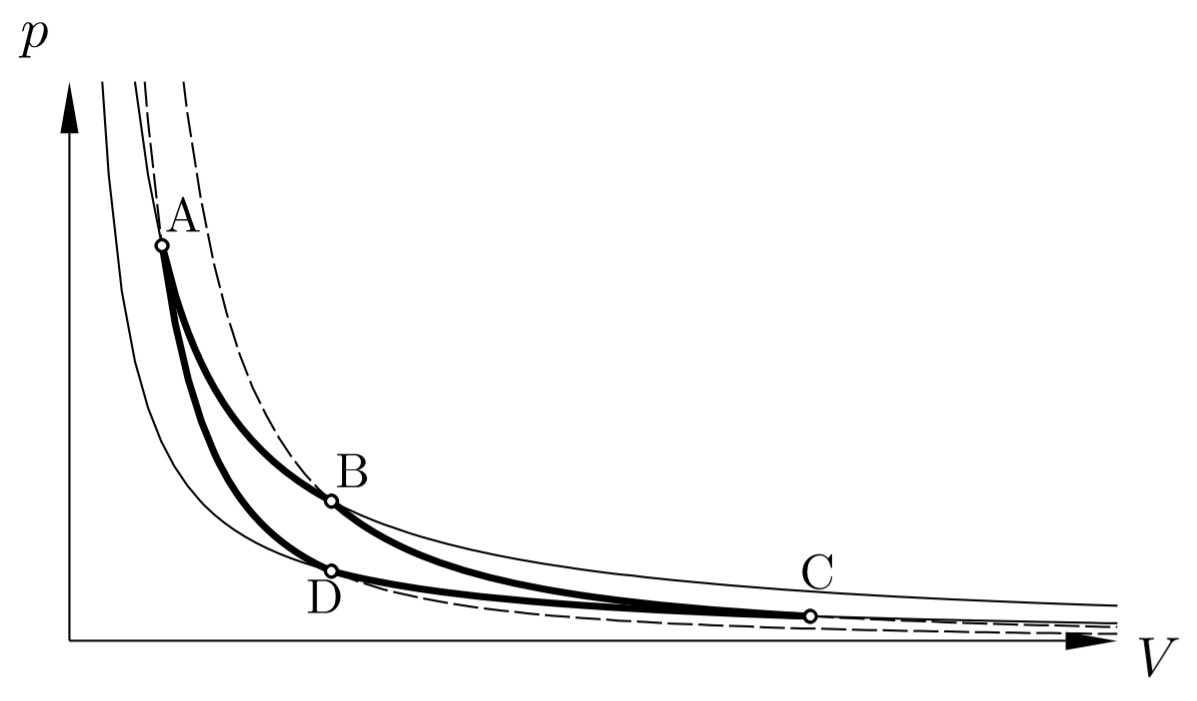
\includegraphics[width=8cm]{adia_pv}
	\centering
	\caption{A p-V plot of the Carnot cycle.}
	\label{fig:adia_pv}
\end{figure}
\begin{figure}[!htbp]
	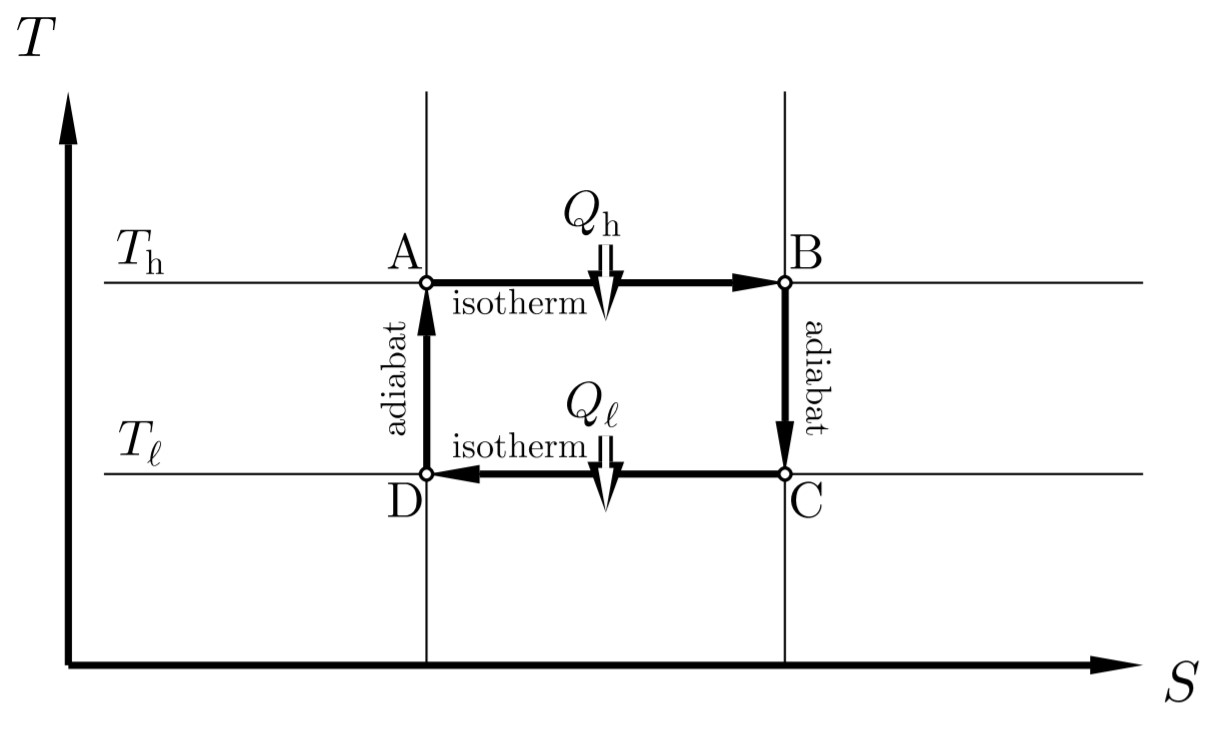
\includegraphics[width=8cm]{adia_ts}
	\centering
	\caption{A T-S plot of the Carnot cycle. 
	$S$ here remains an undefined quantity that we assert is a function of $pV^{\gamma}$ for now.
}
	\label{fig:adia_ts}
\end{figure}
\begin{defi}[Heat engine]
An \textbf{engine} is a system operating a \textit{cyclic} process that converts heat into work. 
\end{defi}
An example of a heat engine is the Carnot engine. 
\begin{defi}[Carnot engine]
A \textbf{Carnot engine} runs on the Carnot cycle, consisting of two heat reservoirs of different temperatures, as shown in \Cref{fig:adia_pv,fig:adia_ts}. 
Thermodynamically, it consists of four alternating reversible isotherms and adiabats. 
Heat only enters and leaves on the isotherms whereas work is performed on all four segments. 
\end{defi}

\begin{thrm}[Work done by Carnot engine]
As this process is cyclic, we can conclude that 
\begin{equation}
W=Q_h-Q_l
\end{equation}
We can write down the governing equations for each segment: 
\begin{subequations}
\begin{align}
A\rightarrow B&:Q_h=RT_h\ln\frac{V_B}{V_A}, \label{car1}\\
B\rightarrow C&:\left(\frac{T_h}{T_l}\right)=\left(\frac{V_C}{V_B}\right)^{\gamma-1}, \label{car2}\\
C\rightarrow D&:Q_l=-RT_l\ln\frac{V_D}{V_C}, \label{car3}\\
D\rightarrow A&:\left(\frac{T_l}{T_lh}\right)=\left(\frac{V_A}{V_D}\right)^{\gamma-1}. \label{car4} 
\end{align}
\end{subequations}
\Cref{car2,car4} lead to
\begin{equation}
\label{car5}
\frac{V_B}{V_A}=\frac{V_C}{V_D}, 
\end{equation}
and dividing \Cref{car1} by \Cref{car3} and substituting in \Cref{car5} gives 
\begin{equation}
\label{carnot_relation}
\frac{Q_h}{Q_l}=\frac{T_h}{T_l}
\end{equation}
\end{thrm}

\begin{defi}[Efficiency]
\begin{equation}
\eta=\frac{W}{Q_h}
\end{equation}
\end{defi}

\begin{lemma}[Efficiency of Carnot engine]
\begin{equation}
\begin{aligned}
\eta_{Carnot}&=\frac{Q_h-Q_l}{Q_h}, \\
\eta_{Carnot}&=\frac{T_h-T_l}{T_h}, \\
&=1-\frac{T_l}{T_h}.  
\end{aligned}
\end{equation}
\end{lemma}

\begin{thrm}[Carnot's theorem]
Carnot's Theorem states that, of all the heat engines working between two given temperatures, none is more efficient than a Carnot engine. 
\end{thrm}

\begin{proof}
We prove the theorem by contradiction. 
Suppose there exists engine E such that $\eta_E>\eta_{Carnot}$. 
Engine E and a Carnot engine running in reverse (having work done \textit{to} it) are connected together with two heat reservoirs at $T_h$ and $T_l$ respectively as shown in \Cref{fig:carnot_thm}. 
We have, 
\begin{equation}
\label{carnot_0}
\begin{aligned}
\frac{W}{Q_h'}&>\frac{W}{Q_h}, \\
Q_h&>Q'_h. 
\end{aligned}
\end{equation}
We also have, 
\begin{equation}
\label{eq:carnot_thm}
\begin{aligned}
W=Q'_h-Q'_l&=Q_h-Q_l, \\
Q_h-Q'_h&=Q_l-Q'_l. 
\end{aligned}
\end{equation}
Now \Cref{eq:carnot_thm} means this compound engine is extracting a positive (due to \Cref{carnot_0}) amount of energy from the low temperature reservoir and dumping the same amount of energy into the high temperature reservoir. 
This is in direct violation of \Cref{L2} and therefore E cannot exist. 
\end{proof}

\begin{figure}[!htbp]
	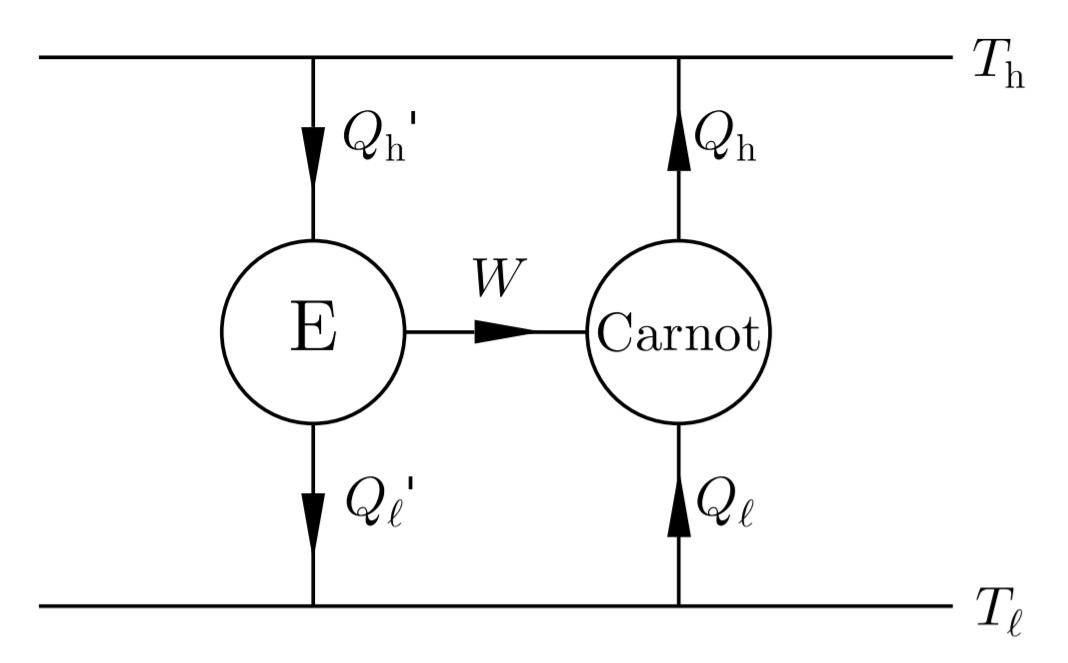
\includegraphics[width=8cm]{carnot_thm}
	\centering
	\caption{Proof of optimality of Carnot engine.}
	\label{fig:carnot_thm}
\end{figure}

\begin{coro}
All reversible engines working between two temperatures have the same efficiency $\eta_{Carnot}$
\end{coro}
\begin{proof}
Suppose there is another reversible engine R such that $\eta_R\leq\eta_{Carnot}$. We run it in reverse and connect to a forward Carnot engine. This arrangement will again transfer heat from the cold reservoir to the hot one, \textit{unless} they have the same efficiency. 
\end{proof}

\begin{prop}[Equivalence of Clausius and Kevin statements]
If a system violates Kelvin's statement of the second law, it also violates Clausius's statement, and \textit{vice versa}. 
\end{prop}
\begin{proof}
As shown in \Cref{kelvin_vio}, by connecting a Kelvin violator, which extracts $Q'_h$ and outputs the same amount of $W$, to a Carnot engine, which extracts $Q_l$, and outputs $Q_h$, we arrive at the same conclusion that this setup violates Clausius statement. 

\begin{figure}[!htbp]
	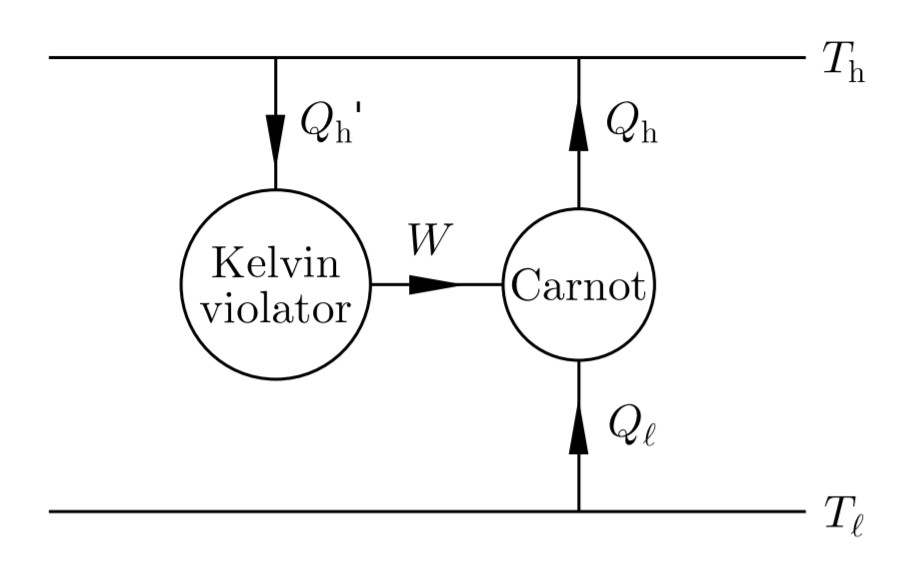
\includegraphics[width=8cm]{kev_vio}
	\centering
	\caption{}
	\label{kelvin_vio}
\end{figure}
\begin{figure}[!htbp]
	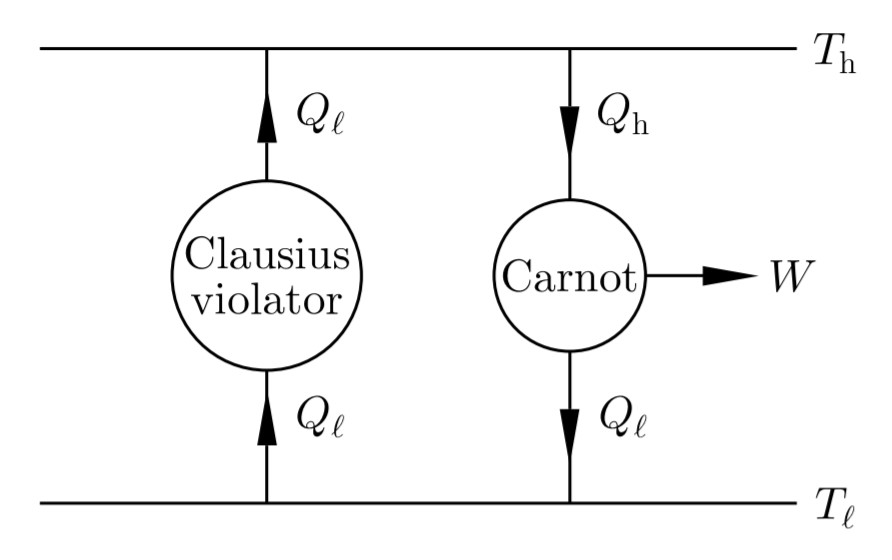
\includegraphics[width=8cm]{clau_vio}
	\centering
	\caption{}
	\label{clau_vio}
\end{figure}

Now, in \Cref{clau_vio} we connect a Clausius violator, transferring $Q_l$ from cold to hot reservoir, 
and a Carnot engine, operating forward. 
The net action of the setup is to convert $Q_h-Q_l$ completely into work, 
hence violating Kelvin's statement.
\end{proof}

\subsubsection{Clausius' theorem}
Consider a Carnot cycle. Heat is \textit{not} conserved around a cycle, however \Cref{carnot_relation} states the important result that 
\begin{equation}
\frac{Q_h}{Q_l}=\frac{T_h}{T_l}, 
\end{equation}
and so we are inspired to define $\Delta Q_{rev}$ as the heat entering the system at each segment, and therefore we have 
\begin{equation}
	\sum_{cycle}\frac{\Delta Q_{rev}}{T}=\frac{Q_h}{T_h}+\frac{\left(-Q_l\right)}{T_l}=0, 
\end{equation}
which means $\Delta Q_{rev}/T$ sums to zero around the cycle. Replcing the sum by an integral we could write 
\begin{equation}
	\oint \frac{\indiff Q_{rev}}{T}=0
\end{equation}
for the Carnot cycle. 

To make a generalised case, we consider a general thermodynamic cycle in \Cref{gen_cyc}(a), where heat $\indiff Q_i$ enters (or leaves, depends on the sign taken up) at a point in the cycle. 
At this point the system is connected to a reservoir at $T_i$. The total work extracted from the cycle is 
\begin{equation}
\Delta W = \sum_{cycle}\indiff Q_i. 
\end{equation}
\begin{figure}[!htbp]
	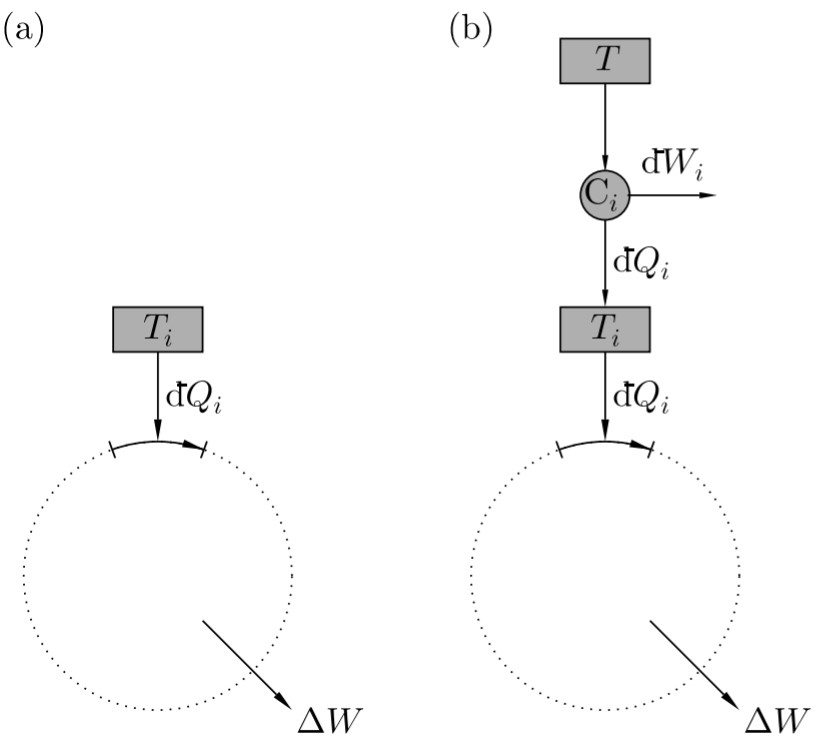
\includegraphics[width=8cm]{gen_cyc}
	\centering
	\caption{}
	\label{gen_cyc}
\end{figure}
Now suppose, as in \Cref{gen_cyc}(b) that all the $\indiff Q_i$ is provided by Carnot engine(s) $C_i$, 
whose input reservoir is fixed at $T$ and output reservoir is the variable $T_i$. 
The Carnot engine itself outputs work $\indiff W_i$. 
We know, for a Carnot engine, 
\begin{equation}
\begin{aligned}
\frac{\text{heat to reservoir at}\ T_i}{T_i}&=\frac{\text{heat from reservoir at}\ T}{T} \\
\frac{\indiff Q_i}{T_i}&=\frac{\indiff Q_i + \indiff W_i}{T} \\
\indiff W_i&=\indiff Q_i \left(\frac{T}{T_i}-1\right). 
\end{aligned}
\end{equation}
For the system to not violate Kelvin's statement of second law, \ie not to convert all the heat into work, as there is no output heat, we must require that 
\begin{equation}
\begin{aligned}
\text{output work}&\leq0 \\
\sum_{cycle}\indiff W_i + \Delta W &\leq 0 \\
T\sum_{cycle}\frac{\indiff Q_i}{T_i}&\leq 0 \\
\oint\frac{\indiff Q}{T}&\leq0, 
\end{aligned}
\end{equation}
which is the \textbf{Clausius inequality}. 

\begin{thrm}[Clausius's theorem]
\label{clau_thrm}
For any closed cycle, $\oint \frac{\indiff Q}{T}\leq0$, where equality necessarily holds for a reversible cycle. 
\end{thrm}

\subsection{Entropy}
We now are in position to introduce the thermodynamic quantity of entropy. 
According to \Cref{clau_thrm}, the integral 
\begin{equation}
\int_A^B \frac{\indiff Q_{rev}}{T}
\end{equation}
is path independent. Therefore the quantity $\indiff Q_{rev}/T$ is an \textit{exact} differential. 
\begin{defi}[Entropy]
Entropy is defined as a state function
\begin{equation}
\dif S=\frac{\indiff Q{rev}}{T}. 
\end{equation}
\end{defi}

\begin{prop}[Adiabatic entropy change]
For an adiabatic process (\textit{defined} as an adiathermal reversible process), 
we have
\begin{equation}
\dif Q_{rev}=0. 
\end{equation}
Hence an adiabatic process involves no change in entropy, \ie isoentropic. 
\end{prop}

\begin{thrm}[Entropy inequality]
Consider a cycle with a reversible and an irreversible segment, 
\Cref{clau_thrm} gives that 
\begin{equation}
\begin{aligned}
	\oint\frac{\indiff Q}{T}&\leq0 \\
	\int^B_A\frac{\indiff Q}{T}+\int^A_B\frac{\indiff Q_{rev}}{T}&\leq0 \\
	\int^B_A\frac{\indiff Q}{T}&\leq\int^B_A\frac{\indiff Q_{rev}}{T} \\
	\dif S = \frac{\indiff Q_{rev}}{T}&\geq\frac{\indiff Q}{T}. 
\end{aligned}
\end{equation}
If we consider a thermally isolated system, \ie $\indiff Q=0$, we then have
\begin{equation}
	\dif S \geq0. 
\end{equation}
\end{thrm}

Now we are in a position to revisit the first law: 
\begin{thrm}[The first law]
For a reversible change only, we have that 
\begin{subequations}
\begin{align}
\indiff Q&=T\dif S \\
\indiff W&=-p\dif V. 
\end{align}
\end{subequations}
For an irreversible change $\indiff Q\leq T\dif S$ and $\indiff Q\geq-p\dif V$, but we \textit{always} have that 
\begin{equation}
\dif U=T\dif S-p\dif V. 
\end{equation}
\end{thrm}
We observe that $S$ and $V$ are the \textbf{natural variables} of $U$, 
and that they are both \textit{extensive}. 
$p$ and $T$ however are \textit{intensive} and behave somewhat like \textit{forces}
\section{Mathematical methods}
\subsection{Legendre transforms}
This subsection is adapted from \cite{lgd_wiki,lgd_paper} and Appendix F of \cite{dill}. \\
Legendre transform, as we will see, is really just a long way to say 'In a right-angled triangle, the slope (tangent) times the adjacent side equals the opposite side'. \\
For a function $F(x)$, we have all the information of the function $F$ stored as ordered pairs of values $(x_i,F(x_i))$. There are many ways to store the same information of the function, one of which is through the gradient. For a function $F$ whose second derivative is always positive, \ie $F$ is monotonously increasing, the gradient $s(x)=\diff {F(x)}/x$ is one-one to $x$, therefore we can invert it to get a single-valued function $x(s)$. 
\begin{figure}[!htbp]
	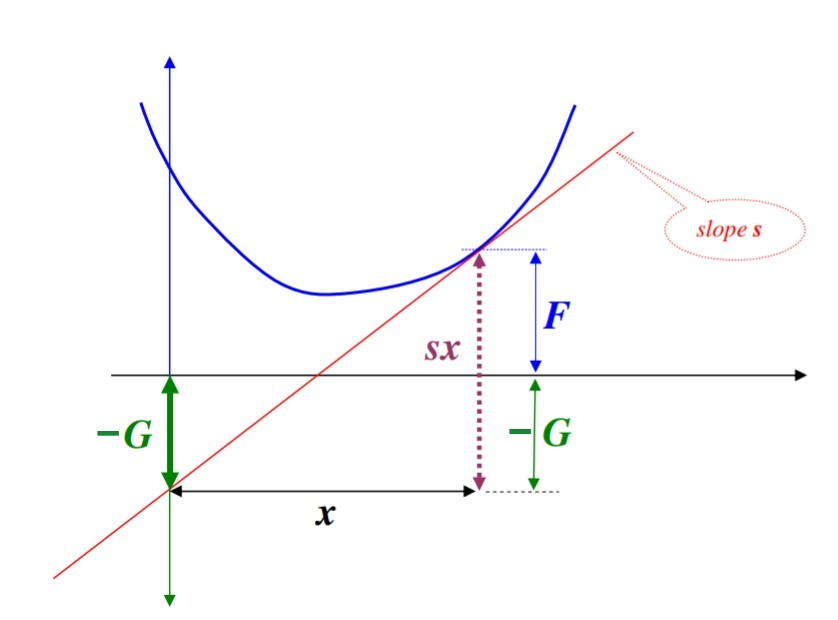
\includegraphics[width=8cm]{legendre1}
	\centering
	\caption{Sometimes the opposite sign convention for $G$ is used to confer more symmetry.}
	\label{legendre1}
\end{figure}
\begin{defi}[Legendre transform]
As shown in \Cref{legendre1}, we are inspired to write
\begin{equation}
sx=F+(-G).
\end{equation}
Rearranged and showing explicitly the functional relationships, 
\begin{equation}
\label{legendre}
G(s)=F(x(s))-sx(s),
\end{equation}
with $-G(s)$ (note the negative sign) known as the Legendre transform of $F(x)$.
This is, at the root of it, just the geometrical statement at the beginning of the section. 
\end{defi}
\begin{prt}[Inverse]
The inverse of the Legendre transform is the starting function, \ie the Legendre transform is its own inverse. We can see this by starting with 
\begin{equation}
y(s)=-\diff Gs
\end{equation}
and inverting the monotonic function $y(s)$ to $s(y)$. 
We then construct the Legendre transform, $H(y)$ of $G(s)$:
\begin{equation}
\begin{aligned}
H(y)&=G(s(y))-ys(y)\\
G&=H-sy
\end{aligned}
\end{equation}
Comparison with \Cref{legendre} reveals that we can identify $\{H,y\}$ with $\{F,x\}$.
This gives us a recursive relation
\begin{subequations}
\begin{align}
s(x)&=\diff Fx \label{lgd_1}\\
x(s)&=-\diff Gs. \label{lgd_2}
\end{align}
\end{subequations}
\Cref{lgd_2} can actually be obtained by differentiating \Cref{legendre}:
\begin{equation}
\diff{G(s)}{s}=\diff{F(x(s))}{s}-x(s)-s\diff xs=-x(s)-s\diff xs+\diff Fx\diff xs=-x(s).
\end{equation}
The symmetric is perhaps best displayed as 
\begin{equation}
\label{lgd_symm}
-G(s)+F(x)=sx.
\end{equation}
Make no mistake here - there is only one independent variable: \textit{either} $x$ \textit{or} $s$, with the other variable written as a function of it. The pair of variables $x$ and $s$ are called \textit{conjugate} variables. 
\end{prt}
\begin{prt}[Extrema]
Remembering that $F$ is defined upwards positive and $G$ downwards positive, as shown in \Cref{legendre1}, we have
\begin{subequations}
\begin{align}
F_{\text{min}}&=-G(0)\\
-G_{\text{min}}&=-F(0).
\end{align}
\end{subequations}
This can be expressed in a more symmetrical form, with the RHS in \Cref{lgd_symm} vanishing in either case: 
\begin{equation}
-G(0)+F(x_{\text{ext}})=0\ \ \ \text{and}\ \ \ -G(s_{\text{ext}})+F(0)=0.
\end{equation}
\end{prt}
We now look at functions of more than one variables, for example, $F(x,y)$. 
We require that $F$ is convex in $x$ for all $y$ and vice versa.
The differential is 
\begin{equation}
\dif F=\diffp Fx \dx + \diffp Fy \dif y\equiv p\dx+v\dif y,
\end{equation}
where $\{p,x\}$ and $\{v,y\}$ are conjugate pairs of variables, and $p$ and $v$ can be understood as the gradient in the two basis vector directions. \\
The Legendre transform aims, again, to swap one variable for its conjugate variable, say $x$ for $p$. 
So essentially we `flatten' a multivariate function into one dimension and the Legendre transform is 
\begin{equation}
G(p,y)\equiv F\bigr(x(p),y\bigl)-px(p).
\end{equation}
We see in the differential form that indeed the independent variable $x$ is switched into $p$:
\begin{equation}
\dif G=\dif F-p\dx-x\dif p=-x\dif p+v\dif y.
\end{equation}
We can identify
\begin{subequations}
\begin{align}
x&=-\diffp Gp \\
v&=\diffp Gy.
\end{align}
\end{subequations}
\begin{wex}
\label{wex_enthalpy}
The internal energy is
\begin{equation}
U=U(S,V,\bvec{N}), 
\end{equation}
with total differential given by
\begin{equation}
dU=T\dif S-P\dif V+\sum \mu_i\dif N_i
\end{equation}
We know from \Cref{diff_p} that $-p$ (again note the negative sign) and $V$ are \textit{defined} by the foundamental thermodynamic equations to be conjugate variables. 
We therefore wish to define a new quantity $H=H(S,p,\bvec{N})$ via a Legendre transform:
\begin{equation}
H(S,p,\bvec{N})\equiv U+pV.
\end{equation}
We can immediately recover from the properties of Legendre transforms that
\begin{subequations}
\begin{align}
V&=\diffp Hp\\
T&=\diffp HS\\
\mu_i&=\diffp{H}{N_i},
\end{align}
\end{subequations}
where subscripts are omitted for clarity. \\
The function $H$ being a Legendre transform of $U$, encodes the exact same information as $U$ but are easier to work with in situations where pressure is constant, as the total differential simplifies. 
\end{wex}
\subsection{Euler-Maclaurin formula}
This is adapted from \cite{emform}. \\
We wish to approximate a sum 
\begin{equation}
S(n)=\sum^{n}_{k=0}f(k)
\end{equation}
by an integral of the form
\begin{equation}
\label{sigman}
\sigma(n)=\int^n_0 f(x)\dx. 
\end{equation}
But this is inaccurate for fast changing sums and it'll be more accurate to 
approximate behaviour of the function near each integer value, which is to say 
that we write the integral this way
\begin{equation}
\sigma(n)=\int^1_0[f(0+x)+f(1+x)+f(2+x)+\cdots+f(n-1+x)]\dx.
\end{equation}
We approximate the behaviour of the function about each integer with a Taylor 
series expansion:
\begin{equation}
f(k+x)=\sum^{\inf}_{j=0}\frac{f^{(j)}(k)}{j!}x^j, 
\end{equation}
whose integral from $0$ to $1$ is 
\begin{equation}
\int^1_0 f(k+x)\dx=\sum^{\inf}_{j=0} \frac{f^{(j)}(k)}{(j+1)!}
\end{equation}
So,
\begin{equation}
\label{sigman2}
\sigma(n)=\sum^{\inf}_{m=0}\frac{S^{(m)}}{(m+1)!}.
\end{equation}
Taking derivative of \Cref{sigman2} we have 
\begin{equation}
\sigma^{(j)}(n)
\end{equation}

\subsection{Homogeneous functions}
\label{homofun}
A polynomial
\begin{equation}
  a_0+a_1x+a_2x^2+\dots+a_nx^n
\end{equation}
is of degree $n$. A polynomial is said to be homogeneous of degree $n$ if all its terms are of the same degree $n$, for example,
\begin{equation}
  x^2+5xy+13y^2
\end{equation}
is homogeneous of degree $2$. The same idea can be extended to functions: if for arbitrary $\lambda$
\begin{equation}
  f(\lambda x)=\lambda^nf(x)
\end{equation}
$f$ is said to be homogeneous of degree $n$ in the variable $x$, and
\begin{defi}[Intensive and extensive variables]
Intensive functions are homogeneous of degree zero and extensive functions are homogeneous of degree one.
\end{defi}
Now consider 
\begin{equation}
  S=S(U,V,n)
\end{equation}
physically, entropy is extensive, so we can write
\begin{equation}
  S(\lambda U,\lambda V,\lambda n)=\lambda S(U,V,n)
\end{equation}
If we choose $\lambda=1/n$ we can write
\begin{equation}
  S(\tfrac{U}{n},\tfrac{V}{n},1)\equiv S_m(U_m,V_m)=\frac{1}{n}S(U,V,n)
\end{equation}
so
\begin{equation}
  nS_m(U_m,V_m)=S(U,V,n)
\end{equation}
This illustrates why $\lambda$ is known as the \emph{scaling function}.

\section{Free energies}
\label{free_energy}
This section is adapted from \cite{dill}. \\
In laboratory conditions, microscopic, extensive quantities such as $S$, $U$ and $\bvec{N}$ is difficult to keep track of at boundaries of systems. 
Instead we can control and keep track of macroscopic, intensive quantites such as $p$ and $T$. 
This makes the use of $U(S,V,\bvec{N})$ or $S(U,V,\bvec{N})$ rather cumbersome. 
However, the second law still applies and as such we can devise new extrumum principles to find conditions of equilibrium. 

\subsection{Helmholtz free energy}
\subsubsection{Inspiration}
\label{A_insp}
Imagine a test tube in a water bath at a fixed temperature $T$, which act as a thermal reservoir. Therefore we need to find a function $A$ whose natural variables are $(T,V,\bvec{N})$ for us to construct a new extremum principle. \\
Now assume that the combined heat bath-test tube system isolated from its surroundings, equilibrium is predicted by the state of maximum entropy $S(U,V,\bvec{N})$. Any change towards equilibrium must have that
\begin{equation}
\label{sbathstt}
\dif S_{\text{combined system}}=\dif S_{\text{bath}}+\dif S_{\text{test tube}}\geq0.
\end{equation}
Since the combined system is isolated, 
\begin{equation}
\label{ubathutt}
\dif U_{\text{bath}}+\dif U_{\text{test tube}}=0.
\end{equation}
The fundamental equation gives 
\begin{equation}
\dif S_{\text{bath}}=\left(\frac{1}{T}\right)\dif U+\left(\frac{p}{T}\right)\dif V-\left(\frac{\mu}{T}\right)\dif N=\left(\frac{1}{T}\right)\dif U_{\text{bath}}=-\frac{\dif U_{\text{test tube}}}{T}, 
\end{equation}
where the second equality comes from \Cref{ubathutt}. Applying \Cref{sbathstt} further results in
\begin{subequations}
\begin{align}
\dif S_{\text{test tube}}-\frac{\dif U_{\text{test tube}}}{T}&\geq0\\
\dif U_{\text{test tube}}-T\dif S_{\text{test tube}}&\leq0, 
\end{align}
\end{subequations}
where we have successfully obtained a relation only in terms of the test tube quantities. We therefore define 
\begin{defi}[Helomoltz free energy]
\begin{equation}
A\equiv U-TS, 
\end{equation}
with differential 
\begin{equation}
\dif A=\dif U-T\dif S-S\dif T=\dif U-T\dif S\ \ \ \text{at constant temperature.}
\end{equation}
Therefore we see that Helmholtz free energy is essentially the amount of reversible work obtainable from an isothermal and isochoric system:
\begin{equation}
\begin{aligned}
\dif A&=\indiff Q+\indiff W-T\dif S\\
&=\indiff W, 
\end{aligned}
\end{equation}
where we assumed reversibility, which extracts most amount of work.
\end{defi}
\begin{prt}[Condition of equilibrium]
We can see that the condition in \Cref{sbathstt} is fulfiled when 
\begin{equation}
(\dif A)_T\leq0. 
\end{equation}
This means that equilibrium is reached when $A$ is at a minimum.
\end{prt}
\begin{prt}[Fundamental equation]
\begin{equation}
\dif A=-S\dif T-p\dif V+\sum_{j=1}^M\mu_j\dif N_j
\end{equation}
And we can trivially obtain more definitions:
\begin{subequations}
\begin{align}
S&=-\diffp FT[V,\bvec{N}]\\
p&=-\diffp FV[T,\bvec{N}]\\
\mu_j&=\diffp{A}{N_j}[V,T,N_{i\neq j}]. 
\end{align}
\end{subequations}
On the surface this definition seems strange because we need to hold $T$ and $V$ constant and we're only left with the chemical potential term. It is true that if we're looking at a one-component non-reacting system, if we fix $T$ and $V$, no change can take place. But in a multi-component, reacting mixture with fixed $T$ and $V$ we have 
\begin{equation}
\dif A=\sum_{j=1}^M\mu_j\dif N_j
\end{equation}where $A$ can depend on $T$ and $V$ in the \textit{equation of state}, we have the chemical potential terms in the differentials, which changes to minimise the entropy. The following two examples illustrates this idea.
\end{prt}
\subsubsection{A microscopic look at Helmholtz I: Dimerisation}
Suppose $N=2$ gas particles are contained in a test tube of $V$ lattice sites in a row at $T$. We ask under what conditions will the two associate into a dimer. We compute the free energies of monomer and dimer states and compare them. \\
\textbf{Dimers: }Suppose when two monomer sit on adjacent sites a 'bond energy' $U=-\epsilon$ is additionally introduced. \\
Within $V$ sites, multiplicity for a dimer is 
\begin{equation}
W_{\text{d}}=V-1\approx V. 
\end{equation}
The Helmholtz free energy is then given as 
\begin{equation}
A_{d}=U_{d}-TS_{d}=-\epsilon-kT\ln V.
\end{equation}
\textbf{Monomers: }There is no energy of interaction, and the multiplicity is 
\begin{equation}
W_{m}=W_{\text{total}}-W_{d}=\frac{V!}{(2!)(V-2)!}-(V-1)=\left(\frac{V}{2}-1\right)(V-1)\approx\frac{V^2}{2}.
\end{equation}
So the free energy is
\begin{equation}
A_m=-kT\ln\left(\frac{V^2}{2}\right).
\end{equation}
Temperature at which both are equally stable is, after some algebra
\begin{equation}
T_0=\frac{\epsilon}{k\ln(V/2)}.
\end{equation}
Had we only maximised entropy we would conclude that the dimers will never even form, hence missing out on the significant role energy plays at lower temperatures here. 
\subsubsection{A microscopic look at Helmholtz II: Polymer collapse}
\label{polymer_collapse}
\begin{figure}[H]
	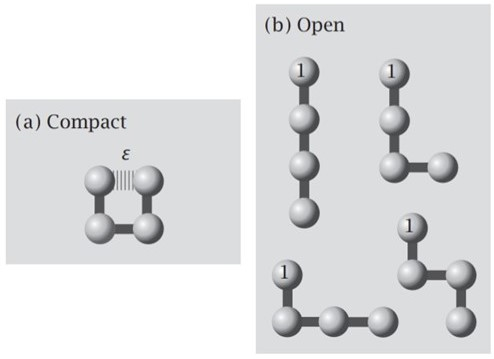
\includegraphics[width=8cm]{polymer_collapse}
	\centering
	\caption{The two energy levels.}
	\label{fig:polymer_collapse}
\end{figure}
Consider a two-dimensional model polymer with four monomers in a closed test tube solution in a bath at $T$ and the ends of the polymer are attracted to each other by $U=-\epsilon$. The multiplicity is $1$ as only one conformation can result in the close-ring polymer. The open-ring state has $4$ other multiplicities. We compute the free energies:
\begin{subequations}
\begin{align}
A_c&=-\epsilon-kT\ln 1=-\epsilon\\
A_o&=-kT\ln 4.
\end{align}
The collapse temperature $T_0$ is given as
\begin{equation}
T_0=\frac{\epsilon}{k\ln 4}.
\end{equation}
\end{subequations}
We note that for this process, 
\begin{subequations}
\begin{align}
\Delta F_{\text{collapse}}&=-\epsilon+kT\ln 4 \\
\Delta U_{\text{collapse}}&=-\epsilon\\
\Delta S_{\text{collapse}}&=-k\ln 4
\end{align}
\end{subequations}
As no volume change is involved, in a reversible process no work is done and $\Delta U=-\epsilon$ and the process is exothermic at all temperature. 
\subsection{Enthalpy}
The enthalpy is most commonly obtained as a Legendre transform of $U$ as explained in \Cref{wex_enthalpy}. We can write out the total differential:
\begin{equation}
\dif H=T\dif S+V\dif P+\sum\mu_j\dif N_j.
\end{equation}
At constant pressure, with a non-reacting mixture, we can write 
\begin{equation}
\dif S=\frac{\dif H}{T}.
\end{equation}
By way of the argument used in \Cref{A_insp}, we introduce two systems $A$ and $B$, 
with $A$ being an open test tube and $B$ the surroundings, acting as a pressure reservoir. Any change towards \eqm will have 
\begin{equation}
\dif S_{A+B}=\dif S_A+\dif S_B\geq0.
\end{equation}
Because $B$ is also a temperature reservoir, we write 
\begin{equation}
\dif S_B=-\frac{\indiff Q_A}{T}.
\end{equation}
Combined, we have
\begin{equation}
\dif S_A-\frac{\indiff Q_A}{T}\geq0.
\end{equation}
Under constant pressure we have
\begin{equation}
\dif H=\dif U+p\dif V-V\dif p=\indiff Q-p\dif V+p\dif V-V\dif p=\indiff Q, 
\end{equation}
and as such
\begin{equation}
T\dif S_A-\dif H\geq0. 
\end{equation}
For tending to equilibrium inside $A$, we require that
\begin{equation}
\dif S_A\geq0,
\end{equation}
therefore 
\begin{equation}
\frac{\indiff Q_A}{T}\leq0.
\end{equation}
So finally we have that
\begin{equation}
\dif H\leq0
\end{equation}
for processes to tend to equilibrium at constant pressure.
\subsection{Gibbs free energy}
To get a function that is minimised at equilibrium at constant pressure and temperature, we perform a Legendre transform on $H(S,p,\bvec{N})$ to get $G(T,p,\bvec{N})$, nothing that $T$ and $S$ are a conjugate pair and the usual sign convention applies:
\begin{equation}
G(T,p,\bvec{N})=H-TS.
\end{equation}
The total differential is given as 
\begin{equation}
\dif G=-S\dif T+V\dif p+\sum\mu_j\dif N_j.
\end{equation}
At constant pressure and temperature, 
\begin{equation}
\dif G=\dif H-T\dif S=\indiff Q-T\dif S.
\end{equation}
Invoking Clausius theorem we can show the equilibirum condition, but to do so explicitly, we use the second law, for 
\begin{equation}
\dif S_{A+B}=\dif S_A+\dif S_B=\dif S_A-\frac{\indiff Q_A}{T}\geq0, 
\end{equation}
under constant pressure and temperature, this becomes
\begin{equation}
\begin{aligned}
T\dif S_A-\dif H_A&\geq0\\
(\dif G)_{p, T}&\leq0.
\end{aligned}
\end{equation}
Therefore $G$ is minimised at equilibrium. \\
It is called `free energy' because it shows how much non-mechanical work can be extracted, which is important in chemistry and biology, again we assume constant pressure and temperature: 
\begin{subequations}
\begin{align}
\dif G&=\dif U+p\dif V-T\dif S\\
&=T\dif S-p\dif V+\indiff W_x+p\dif V-T\dif S\\
&=\indiff W_x, 
\end{align}
where we assume the process is reversible, and the $x$ subscript means other forms of work like electrical work.
\end{subequations}
\subsection{More on thermodynamic functions}
\subsubsection{Functional dependencies}
Below we give a summary of the fundamental functions. \\
\begin{table}[H]
\resizebox{\textwidth}{!}{
\begin{tabular}{c c l l l}
\hline
Function & Extremum at eqm & Fundamental equation & Definition & Useful for \\ \hline
$U(S,V,\bvec{N})$ & Minimum & \(\displaystyle \dif U=T\dif S-p\dif V+\sum\mu_j\dif N_j\) &\ &\ \\ 
$S(U,V,\bvec{N})$ & Maximum & \(\displaystyle \dif S=\lf(\frac{1}{T}\rt)\dif U+\lf(\frac{p}{T}\rt)\dif V+\sum\lf(\frac{\mu_j}{T}\rt)\dif N_j\)&\ &\ \\ 
$H(S,p,\bvec{N})$ & Minimum & \(\displaystyle \dif H=T\dif S+V\dif p+\sum\mu_j\dif N_j\)& $H\equiv U+pV$ & Const $S$ and $p$, $\dif H=\dif U$ \\ 
$A(T,V,\bvec{N})$ & Minimum & \(\displaystyle \dif A=-S\dif T-p\dif V+\sum\mu_j\dif N_j\)& $A\equiv U-TS$ & Const $T$ and $V$, $\dif A=\indiff W$\\ 
$G(T,p,\bvec{N})$ & Minimum & \(\displaystyle \dif G=-S\dif T+V\dif p+\sum\mu_j\dif N_j\)&$G\equiv H-TS\equiv A+pV$ & Const $T$ and $p$, $\dif G=\indiff W_x$\\ \hline
\end{tabular}
}
\end{table}
We should be aware that, for example the function $U$ in $A=U-TS$ is not $U(S,V,\bvec{N})$ but instead takes on the arguments of $A$ such that $U=U(T,V,\bvec{N})$. 
This is why minimising $U(T,V,\bvec{N})$ or maximising $S(T,V,\bvec{N})$ individually does not give us \eqm but only their sum in this specific functional form, when minimised, gives equilibrium. \\
We illustrate this idea by considering 
\begin{equation}
G(T,p,\bvec{N})=H(T,p,\bvec{N})-TS(T,p,\bvec{N}).
\end{equation}
$H$ and $S$ here are non-fundamental functions, but they are useful in that they can be conveniently measured and calculated. Now because at constant pressure, 
\begin{equation}
C_p=\lf(\frac{\indiff Q}{\dif T}\rt)_p=\diffp HT[p]=T\diffp ST[p],
\end{equation}
we can write that
\begin{subequations}
\begin{align}
\Delta H(T,p)&=\int^{T_B}_{T_A}C_p(T)\dif T \\
\Delta S(T,p)&=\int^{T_B}_{T_A}\frac{C_p(T)}{T}\dif T.
\end{align}
\end{subequations}
From a series of constant-pressure heat capacity experiments one can obtain $G(T,p)$. \\
From constant-volume heat capacity experiments one can similarly obtain $A(T,V)=U(T,V)-TS(T,V)$ since we know that at constant volume,
\begin{equation}
C_V=\diffp UT[V]=T\diffp ST[V],
\end{equation}
we can write 
\begin{subequations}
\begin{align}
\Delta U(T,V)&=\int^{T_B}_{T_A}C_V(T)\dif T \\
\Delta S(T,V)&=\int^{T_B}_{T_A}\frac{C_V(T)}{T}\dif T.
\end{align}
\end{subequations}
\subsubsection{Non-standard states}
We can further write, for ideal mixtures,
\begin{equation}
\begin{aligned}
  \dif G&=\frac{nRT}{p}\dif p\\
  \int^{p_2}_{p_1}\dif G&=\int^{p_2}_{p_1}\frac{nRT}{p}\dif p\\
  G(p_2)-G(p_1)&=nRT\ln\frac{p_2}{p_1}\\
  G(p)&=G^{\circ}+nRT\ln\frac{p}{p^{\circ}}
\end{aligned}
\end{equation}
For ideal gases, the chemical potential is the molar Gibbs energy, so we can always write
\begin{equation}
  \mu_i(p_i)=\mu_i^{\circ}+RT\ln\frac{p_i}{p^{\circ}}
\end{equation}
and a parametric ($\mu(p)\rightarrow\mu(c(p))$) substitution gives
\begin{equation}
  \mu_i(c_i)=\mu_i^{\circ}+RT\ln\frac{c_i}{c^{\circ}}
\end{equation}
And for the generic reaction
\begin{equation}
  \ch{$\nu$_AA + $\nu$_BB <=> $\nu$_MM + $\nu$_NN}
\end{equation}
with some algebra we get
\begin{equation}
\label{stdgibbsp}
  \Delta_rG^{\circ}=-RT\ln K_p
\end{equation}
and also
\begin{equation}
\label{stdgibbsc}
  \Delta_rG^{\circ}=-RT\ln K_c
\end{equation}
\subsubsection{Gibbs-Helmholtz equation}
For the function $G/T$, we can always write, with chain rule:
\begin{equation}
  \diffp{}{T}(GT^{-1})=T^{-1}\diffp GT-T^{-2}G
\end{equation}
noting that $\diffp G/T=-S$ by definition, we proceed:
\begin{equation}
\begin{aligned}
  \diffp{}{T}(GT^{-1})&=-ST^{-1}-T^{-2}(H-TS)\\
  &=-\frac{H}{T^2}
\end{aligned}
\end{equation}
where we have derived the
\begin{thrm}[Gibbs-Helmholtz equation]
The equation states that
\begin{equation}
  \diffp{}{T}\lf(\frac{G}{T} \rt)=-\frac{H}{T^2}
\end{equation}
\end{thrm}
From this we can derive the van't Hoff equation
\begin{thrm}[van't Hoff equation]
The equation states that
\begin{equation}
  \diffp{\ln K}{T}=\frac{\Delta_rH^{\circ}}{RT^2}
\end{equation}
\end{thrm}
\begin{proof}
  The free energies in Gibbs-Helmoholtz equation can be replaced by changes (over a reaction):
  \begin{equation}
     \diffp{}{T}\lf(\frac{\Delta_rG^{\circ}}{T} \rt)=-\frac{\Delta_rH^{\circ}}{T^2}
  \end{equation}
  and invoking \cref{stdgibbsp,stdgibbsc} we can write that
  \begin{equation}
    \diffp{}{T}(-R\ln K)=-\frac{\Delta_rH^{\circ}}{T^2}
  \end{equation}
  which rearranges to give the van't Hoff equation.
\end{proof}


\subsection{The Euler and Gibbs-Duhem equations}
\label{eulergibbs}
\subsubsection{The Euler equation}
Referring to \cref{homofun}, we now consider the internal energy, which again is physically an extensive function so we can write\footnote{We use $n$ here for simplicity but this can be easily converted and extended to $\bvec{N}$}
\begin{equation}
  U(\lambda S,\lambda V,\lambda n)=\lambda U(S,V,n)
\end{equation}
using the chain rule, we can write
\begin{equation}
\begin{aligned}
  U(S,V,n)=&\diffp{U}{(\lambda S)}[V,n]\diffp{(\lambda S)}{\lambda}+\diffp{U}{(\lambda V)}[S,n]\diffp{(\lambda V)}{\lambda}+\diffp{U}{(\lambda n)}[S,V]\diffp{(\lambda n)}{\lambda}\\
  =&\diffp{U}{(\lambda S)}[V,n]S+\diffp{U}{(\lambda V)}[S,n]V+\diffp{U}{(\lambda n)}[S,V]n\\
  =&TS-pV+\mu n
\end{aligned}
\end{equation}
This is known as the \textbf{Euler equation}, which relates all sever thermodynamic variables.\par
We can further extend this to the Gibbs free energy, which can be written as 
\begin{equation}
\begin{aligned}
G&=H-TS=U+pV-TS\\
&=TS-pV+\mu n+pV-TS\\
&=\mu n
\end{aligned}
\end{equation}
Which can be simply extended to
\begin{equation}
  G=\sum_i\mu_iN_i
\end{equation}
This \emph{holds true for all homogeneous systems}, which can be non-ideal.
\subsubsection{The Gibbs-Duhem equation}
The Euler equation(s) might looks strange because the total differential has extra terms that are not present in the master equation, and vice versa. We need to realise that the master equation started from the conservation of internal energy, which tells us that $U(S,V,N)$ must be a state function, and we can take the total differential and make the definitions to get
\begin{equation}
  \dif U=T\dif S-p\dif V+\mu\dif N
\end{equation}
The Euler equation on the other hand is a statement of the extensivity of energy. So both expressions are logical and the only way to reconcile the two is to take the extra terms in the differential form of the Euler equation to be zero:
\begin{equation}
\begin{aligned}
  \dif U&=T\dif S+S\dif T-p\dif V-V \dif p+\mu\dif N+ N\dif\mu\\
&=\underbrace{T\dif S-p\dif V+\mu\dif N}_{\dif U}+\underbrace{S\dif T-V\dif p+N\dif\mu}_{=0}
\end{aligned}
\end{equation}
This gives us
\begin{thrm}[The Gibbs-Duhem relation]
The relation states that
\begin{equation}
  S\dif T-V\dif p+\sum_iN_i\dif\mu_i=0
\end{equation}
Which tells us that the three intensive variables are interrelated, and specifying two variables allows us to compute the third.
\end{thrm}
This can be extended to Gibbs free energy, where $G=\sum_i\mu_iN_i$ and the master equation is $\dif G=-S\dif T+V\dif p+\sum_i\mu_i\dif N_i$, and we can conclude
\begin{equation}
  S\dif T-V\dif p+\sum_iN_i\dif\mu_i=0
\end{equation}
Under constant $T$ and $p$, we have
\begin{equation}
  \sum_iN_i\dif\mu_i=0
\end{equation}
which in the more illustrative case of a binary system, gives us
\begin{equation}
  \dif\mu_B=-\frac{N_A}{N_B}\dif\mu_A
\end{equation}
which shows that chemical potentials are functions of the composition $\bvec{N}$.

\section{Maxwell's relations and mixtures}
Before we dive head in to proper statistical thermodynamics, let's push the classical, differntial approach to its logical end. \\
There are many external constraints besides the likes of pressure and volume that we have been discussing, 
for example, a lipid bilayer can change its surface area, and a rubber band its length. We ask the following questions: 
\begin{itemize}
	\item What is the extra degree(s) of freedom, \ie new variables?
	\item What is the fundamental function and what does it depend on?
	\item What is the condition of equilibrium?
	\item Is the process tending to equilibrium driven by entropy or enthalpy or both? 
\end{itemize}
\subsection{Designing a fundamental equation}
\begin{defi}[Conjugate pairs]
We have introduced the idea of conjugate pairs, but we now generalise the definition:\\
For a generalised extensive variable $X_j$, we have the conjugate force-analogue $F_j$that is an intensive variable given as 
\begin{equation}
\label{conj_force}
F_j=\diffp{U}{X_j}[S,V,\bvec{N},X_{i\neq j}].
\end{equation}
\end{defi}
Now to make the new, augmented internal energy function we just introduce the \textit{intensive} variable into the argument to get 
\begin{subequations}
\begin{align}
U&=U(S,V,\bvec{N},\bvec{X})\\
\dif U&=T\dif S-p\dif V+\sum\mu_j\dif N_j+\sum F_j\dif X_j.
\end{align}
\end{subequations}
Now, although the definition relies on internal energy, it is almost always easier to work with other thermodynamic potentials - 
because they are exactly introduced to make experiments easier. To transform to a suitable potential, we perform Legendre transforms on $U$.
\begin{wex}
Suppose a system can change its surface area independently of its volume. What is the function that identifies the state of equilibrium? \\
\Cref{conj_force} tells us that 
\begin{equation}
\gamma=\diffp{U}{A}[S,V,\bvec{N}],
\end{equation}
where $\gamma$ is conjuate to surface area and is the \textit{surface tension}. 
However this equation is not really useful as we have to control $S$ and $V$, 
which, for example if we are investigating a lipid bilayer \textit{in vivo}, 
we would want to control $T$ and $p$ instead. This is easy as we can just transform
\begin{equation}
U\leftrightarrow G=U+pV-TS,
\end{equation}
and 
\begin{equation}
dG=-S\dif T+V\dif p+\sum\mu_j\dif N_j+\gamma\dif A,
\end{equation}
where 
\begin{equation}
\gamma=\diffp GA[T,p,\bvec{N}], 
\end{equation}
a quantity that is easy to determine experimentally. However the process can be further streamlined with Maxwell's relations.
\end{wex}
\subsection{Maxwell's relations}
Maxwell's relations result from \textit{equivalence of mixed partials}. \\
Suppose we want to find 
\begin{equation}
\diffp Sp[T,\bvec{N}],
\end{equation}
which could be useful for understanding how the entropies of materials change when they are squeezed. 
We identify the independent variables as $T$, $p$ and $\bvec{N}$ 
and identify that the natural function is $G(T,p,\bvec{N})$, with total differential
\begin{equation}
\dif G=-S\dif T+V\dif p+\sum\mu_j\dif N_j.
\end{equation}
To get the desired partial, we see that
\begin{equation}
S=-\diffp GT,
\end{equation}
so
\begin{equation}
-\diffp Sp=\diffp{G}{p,T}=\diffp{G}{T,p}=\diffp VT.
\end{equation}
Therefore we get our (unique) Maxwell's relation that
\begin{equation}
\diffp Sp[T,\bvec{N}]=-\diffp VT[p,\bvec{N}],
\end{equation}
a quantity that is much easier to experimentally determine.
\subsection{Susceptiblities}
\begin{defi}[Susceptibility]
Susceptibility is generally defined as the fractional change in a quantity as a result of an infinitessimal change in another quantity:
\begin{equation}
\sigma=\frac{1}{X}\diffp XL.
\end{equation}
An example would be the thermal expansion coefficient $\alpha$:
\begin{equation}
\alpha=\frac{1}{V}\diffp VT[p],
\end{equation}
the fractional change in the volume of a system with temperature at constant pressure. 
\end{defi}
Coupled with Maxwell's relations, the experimentally easy to determine susceptabilities can usually give insight to hard to measure quantities. For example the thermal expansion coefficient $\alpha$ above, coupled with
\begin{equation}
\diffp Sp[T,\bvec{N}]=-\diffp VT[p,\bvec{N}]
\end{equation}
we can write
\begin{equation}
\alpha=-\frac{1}{V}\diffp Sp[T,\bvec{N}].
\end{equation}
This means if $\alpha\geq0$, increasing pressure orders the system. Further coupled with equations of state like the ideal gas law we can get
\begin{equation}
\alpha=\frac{p}{NkT}\frac{Nk}{p}=\frac{1}{T}\geq0,
\end{equation}
which says that increasing pressure decreases the entropy of an ideal gas. \\
Change in entropy can then be easily calculated at constant pressure:
\begin{subequations}
\begin{align}
&\dif S=\diffp Sp[T,\bvec{N}]\dif p=-\diffp VT[p,\bvec{N}]\dif p=-\alpha V\dif p\\
\imp&\Delta S=-\int^{p_2}_{p_1}\alpha(p)V(p)\dif p.
\end{align}
\end{subequations}
Another example of susceptibility is 
\begin{defi}[Isothermal compressibility]
\begin{equation}
\kappa=-\frac{1}{V}\diffp Vp[T].
\end{equation}
\end{defi}
A further example is about measuring $\diffp U/V[T]$, which should tell us about the cohesive forces in materials. But this is hard to measure. 
We again recruit the help of susceptibilities. We write
\begin{subequations}
\begin{align}
\dif U=\diffp UV[T]\dif V+\diffp UV[V]\dif T \label{difu_susc}\\
\dif S=\diffp SV[T]\dif V+\diffp ST[V]\dif T, \label{difs_susc}
\end{align}
\end{subequations}
substituting \Cref{difs_susc} into $\dif U=T\dif S-p\dif V$ we get
\begin{equation}
\diffp UV[T]\dif V+\diffp UT[V]\dif T=T\lf[\diffp SV[T]\dif V+\diffp ST[V]\dif T \rt]-p\dif V.
\end{equation}
At constant T this reduces to
\begin{equation}
\diffp UV[T]=T\diffp SV[T]-p,
\end{equation}
using the Maxwell relation
\begin{equation}
\diffp SV[T]=\diffp pT[V]
\end{equation}
gives
\begin{equation}
\diffp UV[T]=T\diffp pT[V]-p.
\end{equation}
The quantity $\diffp p/T[V]$ is the \textit{thermal pressure coefficient}. 
For typical liquids, $T\diffp p/T[V]-p$ is negative at high densities and positive at low densities, 
which is exactly the behaviour we expect due to 
the dominance of repulsive forces at high densities and attractive forces at low densities. 
\subsection{Entropic and enthalpic components}
We first look at a rubber band, whose length $L$, an extensive variable with conjugate restroing force $f$, is the new variable to be introduced as an argument of $U$ while $N$ is fixed: 
\begin{equation}
\dif U=T\dif S-p\dif V+f\dif L.
\end{equation}
Our expreriment is to be carried out at constant $T$ and $p$, so $G$ is the natural function to work with. Under a Legendre transform we have
\begin{equation}
\dif G=\dif\ (U+pV-TS)=-S\dif T+V\dif p+f\dif L.
\end{equation}
So we see
\begin{equation}
f=\diffp GL[T,p]=\diffp HL[T,p]-T\diffp SL[T,p],
\end{equation}
meaning the restoring force $f$ is driven by a combination of entropy and enthalpy. 
To make the entropic component easier to measure, we find its Maxwell relationship: 
\begin{equation}
\diffp SL[T,p]=-\diffp{G}{T,L}=-\diffp fT[p,L], 
\end{equation}
and the enthalpic component is simply
\begin{equation}
\diffp HL[T,p]=f-T\diffp fT[p,L],
\end{equation}
both quantities are very easy to obtain from simple experiments. \\
Now we take a look at a Langmuir trough, a liquid container with a bar frictionlessly floating in it. 
On the right side is water and on the left side is water plus a surfactant like phospholipids. 
If a lateral pressure $\pi$ is exerted towards the left, the surfactant surface must change its area, $a$. 
We identify the relevant function to be $G$ and that 
\begin{equation}
\label{g_surf}
\dif G=-S\dif T+V\dif p-\pi\dif A, 
\end{equation}
where the negative sign in front of $\pi$ means the free energy increases as the surfactant layer is compressed, rather like the $pV$ sign convention. 
In an experiment we can determine $\pi(T,a,N)$, with $N$ being the number of surfactant molecules. \\
Suppose $N$ surfactant molecules can occupy $A$ lattice sites on the left side, with a conversion factor $\lambda$ of area per lattice site. 
In the dilute limit of $N\ll A$, 
the multiplicity is 
\begin{equation}
W\approx A^N.
\end{equation}
So
\begin{equation}
\label{s_langmuir}
S(A)=k\ln W=Nk\ln A.
\end{equation}
In \Cref{g_surf} we can partition $\pi$ into the two components again:
\begin{equation}
\label{pi_langmuir}
\pi=-\diffp GA[T,p]=-\diffp HA[T,p]+T\diffp SA[T,p], 
\end{equation}
and we can get a Maxwell relation 
\begin{equation}
\diffp SA[T,p]=-\diffp {G}{T,A}=\diffp{\pi}{T}[p,A].
\end{equation}
From \Cref{s_langmuir}, we have
\begin{equation}
\diffp{\pi}{T}[p,A]=\frac{Nk}{A}, 
\end{equation}
which implies that
\begin{equation}
\pi A=NkT, 
\end{equation}
the two dimensional ideal gas law. 
Comparing with \Cref{pi_langmuir} we see that the pressure is purely entropic. 
However when the surfactant becomes more concentrated 
the molecules might start interacting amongst themselves and an enthalpic element may be seen. 
\subsection{Partial molar properties}
We now look at multicomponent systems such as liquid mixtures and metal alloys.
\begin{defi}[Partial molar volume]
\begin{equation}
v_j=\diffp{V}{n_j}[T,p,n_{i\neq j}], 
\end{equation}
the change in volume when $\dif n_j$ moles of $j$ molecules are added to the system. Alternatively
\begin{equation}
\dif V=\sum_{j=1}^M \diffp{V}{n_j}[T,p,n_{i\neq j}]\dif n_j=\sum v_j\dif n_j
\end{equation}
\end{defi}
Chemical potentials can be variously defined
\begin{equation}
\begin{aligned}
\mu_j&=\diffp{U}{N_j}[V,S,N_{i\neq j}]=\diffp{G}{N_j}[T,p,N_{i\neq j}]\\
&=\diffp{A}{N_j}[T,V,N_{i\neq j}]=\diffp{H}{N_j}[S,p,N_{i\neq j}].
\end{aligned}
\end{equation}
However, the definition of partial molar quantities are defined specifically 
to be quantities measured at constant $T$ and $p$, so
\begin{defi}[Partial molar free energy]
\begin{equation}
\mu_{j,m}=\diffp{G}{n_j}[T,p,n_{i\neq j}]
\end{equation}
\end{defi}
We can divide the partial molar free energy into its partial molar enthalpy and entropy components: 
\begin{equation}
\begin{aligned}
\mu_j&=\diffp{G}{n_j}[T,p,n_{i\neq j}]\\
&=\diffp{H}{n_j}[T,p,n_{i\neq j}]-T\diffp{S}{n_j}[T,p,n_{i\neq j}]\\
&\equiv h_j-Ts_j.
\end{aligned}
\end{equation}
\chapter{Statistical mechanics}
\section{The Boltzmann distribution law}
\subsection{The canonical ensemble}
The canonical ensemble consists of cells of constant $V,T,N$, essentially a massive collection of bubbles sitting in a heat bath, and asks the question of how many of the bubbles will have the same energy. It is important to note that the particles within each cells are allowed to interact. In the derivation below note how we never assume the particles to be independent (interacting).
\subsubsection{Derivation}
Consider an isolated supersystem with a bath (surroundings) and a system we're interested in. We have
\begin{equation}
    E_{\text{tot}}=E_{\text{sys}}+E_{\text{bath}}.
\end{equation}
We now consider two states of the system, \textbf{A}, with $E_\text{bath,A}=E_{\text{tot}}$ and \textbf{B}, with the system in state $m$ with $E_m$. 
The number of microstates available to the supersystem $\Omega_{\text{tot}}$, is constant. We can write, from the postulate of equal probabilities, we can write
\begin{equation}
    P_m\propto\Omega_{\text{bath}}(E_{\text{tot}}-E_m)
\end{equation}
This can look superficially simple but let's think what it actually means: the postulate of equal probabilities only applies to the \emph{supersystem}, which is isolated. So we can only say that the probability of observing the \emph{system} with energy $E_m$ is proportional to the number of microstates that has the bath with that energy. The choice to use the perspective of the bath but not the system is arbitrary now, however a subsequent approximation makes it necessary. \par
To find the exact functional form of $\Omega_{\text{bath}}(E_{\text{bath}})$, we invoke the definition
\begin{equation}
    \diffp SU[V]=\frac{1}{T}
\end{equation}
Considering just the bath, we have
\begin{equation}
    \diff{\ln{\Omega}_{\text{bath}}(E_{\text{bath}})}{E_{\text{bath}}}=\frac{1}{kT}.
\end{equation}
Now we make the important approximation that, in the limit of $E_{\text{tot}}\gg E_m$, we can approximate the derivative with a simple geometric gradient
\begin{equation}
    \frac{\ln \Omega_{\text{bath}}(E_{\text{bath,B}})-\ln\Omega_{\text{bath}}(E_{\text{bath,B}})}{E_{\text{text,B}}-E_{\text{bath,A}}}=\frac{1}{kT}
\end{equation}
and this readily gives 
\begin{equation}
  \Omega_{\text{bath}}(E_{\text{tot}}-E_m)=\Omega_{\text{bath}}(E_{\text{tot}})\exp\lf(\frac{-E_m}{kT} \rt)
\end{equation}
and as $E_{\text{tot}}$ is fixed, we have
\begin{equation}
  P_m=B\exp\lf(\frac{-E_m}{kT} \rt)
\end{equation}
where $B$ is $1/q$, via the same normalisation argument.

\subsection{Derivation of Boltzmann distribution}
\subsubsection{Via a Lagrange multiplier}
We now derive the Boltzmann distribution law again, this time minimising a free energy. 
The problem we solve is essentially the same as the one in \Cref{chapter1}: 
we are given energy states $E_j$ from the physics of the problem, 
and we aim to compute the probabilities $p_j$ that the system is in $j$. \\
We now suppose that $(T,V,N)$ are held constant, with only one species of particles. 
The condition for \eqm is then 
\begin{equation}
\dif A=\dif U-T\dif S=0.
\end{equation}
This looks arbitrary but we can use any free energies as we have demonstrated in 
\Cref{free_energy}, minimising any of them under appropriate conditions 
is equivalent to maximising entropy. \\
Evidently now we need expressions for $\dif S$ and $\dif U$. 
We have the expression for entropy:
\begin{equation}
S(\bvec{p})=-k\sum^{t}_{j=1}p_j\ln p_j, 
\end{equation}
which readily gives
\begin{equation}
\dif S=\sum\diffp{S(\bvec{p})}{p_j}[p_{i\neq j}]=-k\sum^t_{j=1}(1+\ln p_j)\dif p_j.
\end{equation}
\begin{post}[Internal energy]
The internal energy is given as the average over all microscopic states:
\begin{equation}
U=\lgl E\rgl=\sum^{t}_{j=1}p_jE_j.
\end{equation}
\end{post}
We then have
\begin{equation}
\label{du_boltz}
\dif U=\dif \lgl E\rgl=\sum^{t}_{j=1} (E_j\dif p_j+p_j\dif E_j).
\end{equation}
\begin{post}[Energy levels]
Energy levels $E_j$ only depends on volume and number of particles, and unlike $U$ do not depend on $S$ and $T$:
\begin{equation}
E_j=E_j(V,N).
\end{equation}
\end{post}
This means 
\begin{equation}
\dif E_j=\diffp{E_j}{V}\dif V+\diffp{E_j}{N}\dif N=0.
\end{equation}
As both $V$ and $N$ are held constant, 
\begin{equation}
\dif E_j=0, 
\end{equation}
and \Cref{du_boltz} becomes
\begin{equation}
\dif U=\dif \lgl E\rgl=\sum^{t}_{j=1} E_j\dif p_j.
\end{equation}
Now we have our \textbf{objective function}:
\begin{equation}
\dif A=\dif \lgl E\rgl-T\dif S=0,
\end{equation}
and the \textbf{constraint function} is then the usual
\begin{equation}
\begin{aligned}
\sum^{t}_{j=1} p_j&=1\\
\sum^{t}_{j=1} \dif p_j&=0.
\end{aligned}
\end{equation}
We can then write our Lagrange multiplier as
\begin{equation}
\dif A=\sum^{t}_{j=1} \lf[E_j+kT(1+\ln p_j^*)+\lambda \rt]\dif p_j^*=0.
\end{equation}
Thie requires that
\begin{subequations}
\begin{align}
\ln p_j^*&=-\frac{E_j}{kT}-\frac{\lambda}{kT}-1\\
p_j^*&=e^{-E_j/kT}e^{-(\lambda/kT)-1}. \label{pstarred}
\end{align}
\end{subequations}
As $p_j$'s sum to $1$,
\begin{equation}
\label{probsum}
\sum^{t}_{j=1} e^{-E_j/kT}e^{-(\lambda/kT)-1}=1,
\end{equation}
we can divide \Cref{probsum} through \Cref{pstarred} to eliminate $\lambda$, 
and yield the
\begin{thrm}[Boltzmann distribution law]
The law states that
\begin{equation}
\label{bdl}
p_j^*=\frac{\exp(-E_j/kT)}{\sum^t_{j=1}\exp(-E_j/kT)}\equiv\frac{1}{q}\exp(-E_j/kT).
\end{equation}
where $q$ is the partition function and $E_j$ is the energy of \emph{state} $j$. When multiple states have the same energy \ie degenerate, it is convenient to merge them into \emph{levels} of degeneracy $g_i$:
\begin{equation}
  p_i=\frac{g_i}{q}\exp \lf(\frac{-E_i}{kT} \rt)
\end{equation}
\end{thrm}
The Boltzmann distribution law is just a consequence of maximising entropy: given 
total energy, more molecules would have lower energy 
rather than a few having high energies and the rest having zero, 
to maximise total multiplicity.
\subsubsection{From the canonical distribution}
The Boltzmann distribution essentially arise from the canonical distribution when the particles are non-interacting, basically, we now can say that $Q_N=q^N/N!$ for indistinguishable particles, which is what we assume all along anyway. An outline of the proof is given below:\par
If we assume the particles are independent and non-interacting, we can write
\begin{equation}
  Q_N=\frac{q^N}{N!}
\end{equation}
and with 
\begin{equation}
  U=kT^2\diffp {\ln Q_N}{T}
\end{equation}
we can write
\begin{equation}
  U=NkT^2\frac{1}{q}\diffp qT[V]
\end{equation}
where 
\begin{equation}
  q=\sum_i\exp \lf(\frac{-\ep_i}{kT} \rt)
\end{equation}
So 
\begin{equation}
  \diffp qT[V]=\frac{1}{kT^2}\sum_i\ep_i\exp \lf(\frac{-\ep_i}{kT} \rt)
\end{equation}
Substituting this back into the expression for internal energy, we have
\begin{equation}
  U=\frac{N}{q}\sum_i\exp\ep_i\exp \lf(\frac{-\ep_i}{kT} \rt)
\end{equation}
But internal energy is also just the expectation value:
\begin{equation}
  U=\sum_i n_i\ep_i
\end{equation}
So clearly we can identify
\begin{equation}
\begin{aligned}
  n_i&=\frac{N}{q}\exp \lf(\frac{-\ep_i}{kT} \rt)\\
  p_i&=\frac{1}{q}\exp \lf(\frac{-\ep_i}{kT} \rt)
\end{aligned}
\end{equation}
\subsection{Interpretation of partition function}
\subsubsection{Physical meaning of the partition function}
We introduced the partition function, but have not discussed why it's called `partition function'. 
The partition function is 
\begin{equation}
Q\equiv \sum^{t}_{j=1} e^{-E_j/kT}.
\end{equation}
However, it's more commonly expressed in terms of energy differences as experiments often yield those. 
It is then convenient to define the ground-state as zero, $E_1=0$, and write
\begin{equation}
Q=1+e^{-(E_2-E_1)/kT}+e^{-(E_3-E_1)/kT}+\cdots++e^{-(E_t-E_1)/kT}.
\end{equation}
The two forms are equivalent. \\
Now, when the energies for all energy levels are small, \textit{or} the temperature is high, all the states are equally populated and we have that 
\begin{equation}
\frac{E_j}{kT}\rightarrow0\ \imp\ Q\rightarrow t\ \imp\ p_j^*\rightarrow\frac{1}{t}.
\end{equation}
If all the \textit{non-ground state} energies approach infinity, or the temperature approaches zero, the particles can only occupy the ground state:
\begin{equation}
\frac{E_{j\neq1}}{kT}\rightarrow \inf\ \imp\ Q\rightarrow1\ \imp\ p_1^*\rightarrow1.
\end{equation}
In this casem only the ground state becomes \textit{effectively accessible}. \\
So we can see that the partition function gives the number of states that are \emph{effectively} accessible to the system, 
and the magnitude of $E_j/kT$ determines whether or not the state $j$ is \textit{effectively} accessible. 
But beware that the number of accessible states is always the same $t$ and is independent of system varibles as it is fixed by the physics of the situation. 
In contrast, $Q$ is a function of system variables such as $T$. 

\subsubsection{Distinguishability}
\begin{defi}[Distinguishability]
The distinction between distinguishable and indistinguishable particles lies in 
the de Broglie wavelength in comparison of typical particle separation of the 
type of particle in question, and \textit{not in whether the particles are identical or not}. \\
For example, two tennis balls can be identical but occupy distinct locations and can thus be distinguished. 
The same is true for particles fixed in a lattice, which occupy a relatively fixed position. \\
However, two electrons in the He atom have de Broglie wavelengths about the same or larger than the interelectronic separation, hence cannot be distinguished. 
The same goes for particles in a gas, for example. 
\end{defi}
Now we consider systems made of two independent, distinguishable particles $A$ and $B$. 
The energy levels are $E_j$ and is given as a sum of individual energy levels:
\begin{equation}
E_j=\epsilon_i^A+\epsilon_m^B.
\end{equation}
As the two particles are independent, they have independent partition functions,
\begin{equation}
q_A=\sum^{a}_{i=1} e^{-\epsilon_i^A/kT},
\end{equation}
and likewise for $B$. \\
The partition function for the system is the sum of Boltzmann factors $e^{-E_j/kT}$ over all $j=ab$ energy levels:
\begin{equation}
Q=\sum^{t}_{j=1} e^{-E_j/kT}=\sum^{a}_{i=1} \sum^{b}_{m=1} e^{-(\epsilon_i^A+\epsilon_m^B)/kT}=\sum^{a}_{i=1} \sum^{b}_{m=1} e^{-\epsilon_i^A/kT}e^{-\epsilon_m^B/kT}.
\end{equation}
Because the two paricles are distinguishable, all $j=ab$ energy levels are distinct and independent, for example, $A$ in level 26 and $B$ in level 53 is different from $B$ in 26 and $A$ in 53, hence we can write that
\begin{equation}
Q=\sum^{a}_{i=1} e^{-\epsilon_i^A/kT}\sum^{b}_{m=1} e^{-\epsilon_m^B/kT}=q_Aq_B, 
\end{equation}
and in general, for a system with $N$ distinguishable particles, 
\begin{equation}
Q=q^N.
\end{equation}
However, for indistinguishable particles, having $A$ in level 23 and $B$ in level 54 is exactly the same as the other way around, and the better way to specify this 
is to say that `one particle is in level 23 and another in level 54.' 
Therefore, if we were to count distinct energy levels, which is what the partition function is about, 
we should divide the count by $N!$
\footnote{This is an approximation as if the particles coincide on the same energy level, there will not be overcounting, but this is in reality often negligible as the number of accssible levels are usually much larger than number of particles.}:
\begin{equation}
Q=\frac{q^N}{N!}.
\end{equation}


\subsubsection{Gibb's paradox}
Another, and in my opinion, much better justification for dividing by $N!$ comes from \cite{vnd} 
which shows that the division is merely a redefinition and has no 
fundamental justification, it is there to reconcile the statistical mechanical 
and thermodynamical definitions of entropy, the differences of which was revealed 
by the Gibb's paradox, which provides for two isolated box 
with $N$ identical particles and $X$ accessible energy states, separated by an infinitely 
thin and isolating division. Let's call the system before and after removing the division $A$ and $B$, and 
the multiplicities are given as
\begin{subequations}
\begin{align}
S_A&=X^{2N}\\
S_B&=(2X)^{2N}.
\end{align}
\end{subequations}
The change in entropy is 
\begin{equation}
S_B-S_A=2kN\ln 2,
\end{equation}
but the change must be
\begin{equation}
S_B-S_A=\int^B_A \frac{\indiff Q}{T},
\end{equation}
as the gases remain in equilibrium the removal of division is a quasistatic process so the change \textit{must} be zero. 
This is the Gibb's paradox. To resolve it, we must realise that the definition of
\begin{equation}
S=k\ln W
\end{equation}
is for statistical mechanics and not for thermodynamics, and that, indeed the number
of accessible energy levels has increased but this does not correspond well with the usual notion of entropy, hence we need to redefine entropy as
\begin{equation}
S=k\ln\frac{W}{N!}.
\end{equation}
Now, the `new' multiplicities are 
\begin{subequations}
\begin{align}
W_A&=\frac{X^{2N}}{(N!)^2}\\
W_B&=\frac{(2X)^{2N}}{(2N)!}.
\end{align}
\end{subequations}
We apply Stiring's approximation under the assumption of the \textit{thermodynamic limit} of $N\rightarrow\inf$: 
\begin{equation}
\ln n!\approx n\ln n-n
\end{equation}
to show that
\begin{subequations}
\begin{align}
\ln W_A&=2N\ln X-2\ln N!\approx 2N\ln X-2N\ln N+2N \\
\ln W_B&=2N\ln 2X-2\ln (2N)!\approx 2N\ln 2X-2N\ln 2N+2N.
\end{align}
\end{subequations}
The two expressions are equal, and we have resolved the Gibb's paradox. 
This also provides another justification for dividing the partition function by $N!$. 

\subsection{Applications of the Boltzmann distribution}
\subsubsection{Population of states}
We go through partition functions in great detail in \Cref{nststatmech}, and we use the results from there:
\paragraph{Populations of vibrational energy levels}
For a simple harmonic oscillator, the energy levels, with the lowest level set to 0, are
\begin{equation}
  \ep_{\nu}=\nu h\nu_0
\end{equation}
and 
\begin{equation}
  q'_{\text{vib}}=\frac{1}{1-\exp(-h\nu_0/kT)}
\end{equation}
so we have
\begin{equation}
  p_{\nu}=\lf[1-\exp\lf(\frac{-\theta_{\text{vib}}}{T}\rt) \rt]\exp \lf(\frac{-\nu\theta_{\text{vib}}}{T} \rt)
\end{equation}
\paragraph{Populations of rotational energy levels}
For a rigid rotor, the levels are
\begin{equation}
  \ep_J=BJ(J+1)
\end{equation}
and the levels have degeneracies of $(2J+1)$, so
\begin{equation}
  p_J=\frac{2J+1}{q_{\text{rot}}}\exp \lf(\frac{-BJ(J+1)}{kT} \rt)
\end{equation}
In the high temperature limit (reached at very low actual temperatures, so almost always valid), 
\begin{equation}
  q_{\text{rot}}=\frac{T}{\sigma\theta_{\text{rot}}}
\end{equation}
where $\theta_{\text{rot}}=B/k$, we have
\begin{equation}
  p_J=\frac{\sigma\theta_{\text{rot}}}{T}(2J+1)\exp \lf(\frac{-\theta_{\text{rot}}J(J+1)}{T} \rt)
\end{equation}
The degeneracy term wins out the exponential form at small $J$ and so intensity increases at first, but eventually tails out. The maximum can be found by setting $\diff{p_J}/{J}=0$, which gives
\begin{equation}
  J_{\text{max}}=\sqrt\frac{T}{2\theta_{\text{rot}}}-\frac{1}{2} 
\end{equation}
\subsubsection{Density of states}
The density of states $D(\ep)$ is the number of states per energy, or $D(\ep)\dif\ep$ is the number of states between $\ep$ to $\ep+\dif\ep$. It is formally the derivative of number of states, $W(\ep)$, which gives the number of states up to $\ep$:
\begin{equation}
  D(\ep)=\diff{W(\ep)}{\ep}
\end{equation}
We consider the very densely packed case of translational energy states: in a cubical box of side $a$, the energy levels are
\begin{equation}
  E_{n_x,n_y,n_z}=(n_x^2+n_y^2+n_z^2)\frac{h^2}{8ma^2}
\end{equation}
This is reminiscent of the Cartesian expression for a sphere, with $n_x^2+n_y^2+n_z^2$ the squared radius, so the `radius' is given as 
\begin{equation}
  n_{\text{max}}=\lf(\frac{8ma^2\ep}{h^2} \rt)^{1/2}
\end{equation}
However, only the octant corresponding to positive $(x,y,z)$ can be taken as $n_i$'s are nonzero, so the number of states are
\begin{equation}
  W(\ep)=\frac{1}{8}\times\frac{4}{3}\pi n_{\text{max}}^3=\frac{\pi}{6}\lf(\frac{8m\ep}{h^2} \rt)^{3/2}V
\end{equation}
where we wrote $a^3$ as $V$. $D(\ep)$ soon follows:

\begin{thrm}[Density of translational states in a box]
For a cubical box with volume $V$, $D(\ep)$ is given as 
\begin{equation}
  D(\ep)=\diff{D(\ep)}{\ep}=\frac{\pi}{4}\lf(\frac{8m}{h^2} \rt)^{3/2}\ep^{1/2}V
\end{equation}
\end{thrm}
This is a result that will come in handy when we constider the free electron gas model of metal bonding.
\subsubsection{Non-equilibrium states}
The population ratio between states is given as 
\begin{equation}
  \frac{n_1}{n_0}=\exp \lf(\frac{-\Delta\ep}{kT} \rt)
\end{equation}
It is possible to excite population from the lower energy level selectively by methods such as intense radiation, such that $n_1>n_0$ and the temperature is temporarily negative. This is called a \emph{population inversion}, which is important in the working of lasers.
\subsubsection{Maxwell-Boltzmann distribution of velocities}
We adopt the assumptions of the kinetic theory that gas particles can be 
treated as perfect Newtonian particles. The kinetic energy, which is the total energy is given by 
\begin{equation}
\epsilon(v)=\frac{1}{2}mv^2.
\end{equation}
According to the Boltzmann law, the probability $p(v_x)$ that a particle in a container at constant volume and temperature will have volcity $v_x$ in the $x$ direction is 
\begin{equation}
p(v_x)=\frac{e^{-\epsilon/kT}}{\intinf e^{-\epsilon/kT}\dif v_x}, 
\end{equation}
where $\dif v_x$ serves the same role as the rolling index $j$ in \Cref{bdl}. 
We write further that
\begin{subequations}
\begin{align}
p_(v_x)&=\frac{e^{-mv_x^2/2kT}}{\intinf e^{-mv_x^2/2kT}\dif v_x}\\
&=\lf(\frac{m}{2\pi kT} \rt)^{1/2}e^{-mv_x^2/2kT}
\end{align}
\end{subequations}
The \textit{mean-square} velocity is
\begin{subequations}
\begin{align}
\lgl v_x^2\rgl&=\intinf v_x^2p(v_x)\dif v_x\\
&=\lf(\frac{m}{2\pi kT} \rt)^{1/2}\intinf v_x^2e^{-mv_x^2/2kT}\dif v_x\\
&=\lf(\frac{m}{2\pi kT} \rt)^{1/2}\lf(\frac{kT}{m} \rt)\lf(\frac{2\pi kT}{m} \rt)^{1/2} \\
&=\frac{kT}{m}.
\end{align}
\end{subequations}
This means that the average kinetic energy is 
\begin{equation}
\frac{1}{2}m \lgl v_x^2\rgl=\frac{1}{2}kT.
\end{equation}
In three dimensions, because
\begin{equation}
|\bvec{v}|^2=\bvec{v}\cdot\bvec{v}=v_x^2+v_y^2+v_z^2,
\end{equation}
and because all three components are treated as independent,
\begin{equation}
\lgl v^2\rgl=\lgl v_x^2\rgl+\lgl v_y^2\rgl+\lgl v_z^2\rgl,
\end{equation}
so
\begin{equation}
\frac{1}{2}\lgl v^2\rgl=\frac{3}{2}kT.
\end{equation}
As the velocities are independent, the probabilities multiply to give
\begin{equation}
p(v)=p(v_x)p(v_y)p(v_z)=\lf(\frac{m}{2\pi kT} \rt)^{3/2}e^{-mv^2/2kT}.
\end{equation}




\subsection{Thermodynamic properties from partition functions}
\subsubsection{Distinguishable particles}
\textbf{Internal energy}\\
For a system with fixed $(T,V,N)$, to get the internal energy, we remember
\begin{subequations}
\begin{align}
U&=\lgl E\rgl=\sum^{t}_{j=1} p_jE_j\\
&=\frac{1}{Q}\sum^{t}_{j=1} E_je^{-\beta E_j},
\end{align}
\end{subequations}
where $\beta=1/kT$. We note that the sum in the last equality is a derivative of the partition function:
\begin{equation}
\diffp Q\beta=\diffp*{\sum^{t}_{j=1} e^{-\beta E_j}}\beta=-\sum^{t}_{j=1} E_je^{-\beta E_j}.
\end{equation}
Therefore, 
\begin{equation}
U=-\frac{1}{Q}\diffp Q\beta=-\diffp{\ln Q}{\beta}=-\diffp{\ln Q}{T}\diffp{T}{\beta}=kT^2\diffp{\ln Q}{T}
\end{equation}
\textbf{Average particle energy}\\
For distinguishable particles we have $Q=q^N$ so
\begin{equation}
\lgl \epsilon\rgl=\frac{U}{N}=\frac{kT^2}{N}\diffp{\ln q^N}{T}=kT^2\diffp{\ln q}{T}.
\end{equation}
\textbf{Entropy}\\
As entropy is defined as 
\begin{equation}
S=-k \sum^{t}_{j=1} p_j\ln p_j,
\end{equation}
we can get 
\begin{subequations}
\begin{align}
S&=-k \sum^{t}_{j=1} \lf(\frac{1}{Q}e^{-E_j/kT} \rt)\lf[\ln\lf(\frac{1}{Q}\rt)-\frac{E_j}{kT} \rt]\\
&=-k\lf[ \sum^{t}_{j=1} \lf(\frac{1}{Q}e^{-E_j/kT} \rt)\ln\lf(\frac{1}{Q}\rt)-\sum^{t}_{j=1} \lf(\frac{1}{Q}e^{-E_j/kT} \rt)\frac{E_j}{kT} \rt]\\
&=-k\frac{Q}{Q}\ln\lf(\frac{1}{Q}\rt)+\frac{U}{T}\\
&=k\ln Q+\frac{U}{T}
\end{align}
\end{subequations}
\textbf{Free energies and potentials}\\
We have
\begin{equation}
A\equiv U-TS. 
\end{equation}
So obviously,
\begin{equation}
A=-kT\ln Q.
\end{equation}
And more definitions follow:
\begin{equation}
\mu=\diffp AN[T,V]=-kT\diffp{\ln Q}{N}[T,V],
\end{equation}
and so on.
\subsubsection{Indistinguishable particles}
In this case $Q_N=q^N/N!$, and under Stirling's approximation
\begin{equation}
\ln N!=N\ln N-N,
\end{equation}
we can write...\\
\textbf{Internal energy}
\begin{equation}
    \begin{aligned}
   U&=kT^2\diffp{\ln q^N/N!}{T}[V]\\
   &=NkT^2\diffp{\ln q}{T}[V]
    \end{aligned}
\end{equation}
\textbf{Entropy}
\begin{equation}
    \begin{aligned}
    S&=k\ln\frac{q^N}{N!}+\frac{U}{T}\\
    &=Nk\ln q-Nk\ln N+Nk+\frac{U}{T}
    \end{aligned}
\end{equation}
\textbf{Free energy}
\begin{equation}
    \begin{aligned}
    A&=-kT\ln\frac{q^N}{N!}\\
    &=-NkT\ln q+kT(N\ln N-N)
    \end{aligned}
\end{equation}
\textbf{Chemical potential}\\
\begin{equation}
\begin{aligned}
  \mu=\diffp AN[T,V]=-kT\ln\lf(\frac{q}{N} \rt)
\end{aligned}
\end{equation}
\subsection{Examples of the two-state model}
\subsubsection{The Schottky model}
Consider a system with $N$ distinguishable particles with just two energy levels 
for each particle: a ground state with energy zero and an excited state with energy 
$\epsilon=\epsilon_0>0$. This is a widely applicable model such as our polymer or dimer models, 
or in general any excitable particle systems. \\
Here we give a general discussing, aiming to find the average energy $\lgl \epsilon\rgl$, 
the heat capacity $C_V$, the entropy and the free energy per particle, from the partition function, which is given by
\begin{equation}
q=1+e^{-\beta\epsilon_0}.
\end{equation}
$q$ approaches $1$ at low temperatures and $2$ at high temperatures, with probabilities given by
\begin{equation}
p_1^*=\frac{1}{q}\ \ \ \text{and}\ \ \ p_2^*=\frac{e^{-\beta\epsilon_0}}{q}.
\end{equation}
Average energy is 
\begin{equation}
\lgl \epsilon\rgl=\sum p_j^*\epsilon_j=\epsilon_0p_2^*=\frac{\epsilon_0e^{-\epsilon_0/kT}}{1+e^{-\epsilon_0/kT}}.
\end{equation}
Heat capacity is given by
\begin{equation}
C_V=\diffp UT[V,N]=N\diffp{\lgl \epsilon\rgl}{T}[V,N].
\end{equation}
The evaluation of the derivative above is not straightforward, we can make it simpler by writing 
\begin{equation}
N\diffp{\lgl \epsilon\rgl}{T}[V,N]=N\diffp{\lgl \epsilon\rgl}{\beta}\diff{\beta}{T}=\frac{N\epsilon_0^2}{kT^2}\frac{e^{-\beta\epsilon_0}}{(1+e^{-\beta\epsilon_0})^2}.
\end{equation}
\begin{figure}[ht]
	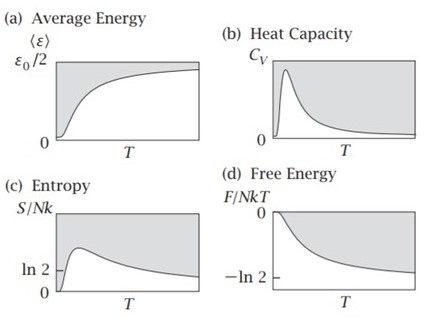
\includegraphics[width=8cm]{schottky}
	\centering
	\caption{}
	\label{fig:schottky}
\end{figure}
As shown in \Cref{fig:schottky} (b), there is a characteristic sharp peak in $C_V$ 
at intermediate temperatures, when the energy of the heat bath can most effectively 
excite the particles in the system. \\
Entropy is obtained by remembering
\begin{subequations}
\begin{align}
S&=k\ln Q+\frac{U}{T}\\
&=Nk\ln (1+e^{-\epsilon_0/kT})+\frac{N\epsilon_0e^{-\epsilon_0/kT}}{T(1+e^{-\epsilon_0/kT})}, 
\end{align}
\end{subequations}
and lastly, free energy:
\begin{equation}
A=-kT\ln Q=-NkT\ln(1+e^{-\epsilon_0/kT}).
\end{equation}
As $\epsilon_0\rightarrow\inf$, the excited states becomes inacessible and so 
$S\rightarrow0$ and $A\rightarrow0$. \\
As $\epsilon_0\rightarrow0$, two states are equally accessible and so 
$S\rightarrow Nk\ln 2$ and $A\rightarrow -NkT\ln 2$. 
\subsubsection{Curie's law of paramagnetism}
Paramagnetic materials are made up of atoms which have negligible dipole-dipole 
as compared to interaction with an applied field. 
Each atom has a magnetic dipole of magnitude $\mu_0>0$, and gives an energy of 
$-\mu_0B$ if the spin is aligned parallel to the field and $+\mu_0B$ if aligned 
antiparallel. Setting the ground state energy to $0$ we have our partition function: 
\begin{equation}
q=1+e^{-2\mu_0B/kT}.
\end{equation}
We would like to calculate the average magnetic moment. The probabilities are
\begin{equation}
p_1^*=\frac{1}{q}\ \ \ \text{and}\ \ \ p_2^*=\lf(\frac{1}{q} \rt)e^{-2\mu_0B/kT}.
\end{equation}
So the average dipole moment is calculated by
\begin{equation}
\lgl \mu\rgl=\mu_0p_1^*+(-\mu_0)p_2^*=\mu_0\frac{1-e^{-2\mu_0B/kT}}{1+e^{-2\mu_0B/kT}}=\mu_0\tanh\lf(\frac{\mu_0B}{kT}\rt).
\end{equation}
The Taylor series expansion gives 
\begin{equation}
\lgl \mu\rgl=\frac{\mu_0^2B}{kT}
\end{equation}
at small $\mu_0B/kT$, meaning high temperature and/or weak field. This is \textbf{Curie's law}. 
This explains the fact that cooling and high field strengths magnetise paramagnets effectively. 
\subsubsection{Modelling a protein loop}
test
\section{The statistical mechanics of simple gases}
\label{nststatmech}
\subsection{Molecular partition function}
\subsubsection{Translational partition function}
The quantum mechanical model of a particle in a potential well provides energy 
levels for such a particle, and the energies are given by
\begin{equation}
\epsilon_n=\frac{nh^2}{8mL^2}, 
\end{equation}
where $L$ is the length of the well. 
So the translational partition function is given by
\begin{equation}
q_{\text{trans}}=\sum^{\inf}_{n=1} e^{-\epsilon_n/kT}=\sum^{\inf}_{n=1} e^{-n^2h^2/(8mL^2kT)}.
\end{equation}
It is customary to define
\begin{defi}[Temperature of degrees of freedom]
Energies associated with degrees of freedom are usually divided by the 
Boltzmann factor and expressed in units of temperature. For example, the 
\textbf{translational temperature} is 
\begin{equation}
\theta_{\text{trans}}=\frac{h^2}{8mL^2k}, 
\end{equation}
such that partition function can be compactly written as 
\begin{equation}
q_{\text{trans}}=\sum^{\inf}_{n=1} e^{-n^2\theta/T},
\end{equation}
If the temperature of a degree of freedom is low, then the partition function 
can be \textit{approximated by an integral}. 
\end{defi}
Evidently, when $\theta/T\ll1$, the ability of the $n^2$ factor of bringing 
the magnitude of the exponential is limited, and a great many Boltzmann's factors 
will be evaluated at around $1$ until very large $n$ is reached. This means 
the partition function, and hence the number of effectively 
populated states is very large. This means we can approximate the sum as an integral: 
\begin{equation}
q_{\text{trans}}=\intinfp e^{(-h^2/8mL^2kT)n^2}\dif n=\lf(\frac{2\pi mkT}{h^2} \rt)^{1/2}L\equiv \frac{L}{\Lambda},
\end{equation}
where $\Lambda=(2\pi mkT/h^2)^{-1/2}$ is the \textbf{thermal wavelength}.
Now, for a 3D box of side lengths $a,b,c$, as the motion in each direction 
is assumed to be \textit{independent}, the wavefunction $\psi(x,y,z)$ can be 
separated into $\psi(x)\psi(y)\psi(z)$, and we can write
\begin{equation}
H\psi(x,y,z)=(H_x+H_y+H_z)\psi(x)\psi(y)\psi(z)=\epsilon_{n_x,n_y,n_z}\psi(x,y,z), 
\end{equation}
where 
\begin{equation}
H\equiv-\frac{\hbar^2}{2m}\lf(\diffp[2]{}{x}+\diffp[2]{}{y}+\diffp[2]{}{z} \rt)+\underbrace{V(x,y,z)}_{=0},
\end{equation}
and 
\begin{equation}
\ep_{n_x,n_y,n_z}=\frac{h^2}{8m}\lf(\frac{n_x^2}{a^2}+\frac{n_y^2}{b^2}+\frac{n_z^2}{c^2} \rt).
\end{equation}
As the energy can be separated into three dimensions (a direct result of the fact 
that their motions are independent, anyway), the Boltzmann factors are multiplied 
and hence can be independently evaluated and so the resulting partition functions 
are just the product of three one-dimentsional partition functions:
\begin{equation}
q_{\text{trans}}=q_xq_yq_z=\lf(\frac{2\pi mkT}{h^2} \rt)^{3/2}V\equiv\frac{V}{\Lambda^3}
\end{equation}
\begin{wex}
For temperature $T=273$K, and the volume $V=2.24\times10^{-2}\text{m}^3$ of one 
mole of gas at $p=1$atm, the translational partiton function is 
\begin{equation}
q_{\text{trans}}=\lf(\frac{2\pi mkT}{h^2} \rt)^{3/2}V.
\end{equation}
Substituting in mass for a single atom computed from molar mass, we have
\begin{equation}
q_{\text{trans}}\approx4.79\times10^{30}\ \text{states per atom}.
\end{equation}
\end{wex}
\subsubsection{Vibrational partition function}
The quantum mechanical harmonic oscillator model gives the energy of a harmonic 
oscillator as 
\begin{equation}
\ep_v=\hbar\omega\lf(v+\frac{1}{2} \rt),\ v=0,1,2,\cdots,
\end{equation}
where $\omega=\sqrt{k/\mu}$. We set the ground state energy 
$\ep_0=\hbar\omega/2$ to $0$, to get the partition function
\begin{equation}
q_{\text{vib}}=\sum^{\inf}_{v=0}e^{-\hbar\omega v/kT}\equiv1+x+x^2+\cdots=(1-x)^{-1}=\frac{1}{1-e^{-\hbar\omega/kT}}.
\end{equation}
We can use the Taylor series expansion because the vibrational temperture, given by
\begin{equation}
\theta_{\text{vib}}=\frac{\hbar\omega}{k}\approx10^3\ \text{K}
\end{equation}
is large enough to make sure that $|x|<1$, which is the condition of convergence for this Taylor series. 
\begin{wex}
Oxygen molecules have a vibrational wavenumber of $1580\ \text{cm}^{-1}$, so
\begin{equation}
\theta_{\text{vib}}=\frac{\hbar\omega}{k}\approx2274\ \text{K}.
\end{equation}
So the partition function at $T=300$ K is 
\begin{equation}
q_{\text{vib}}=\frac{1}{1-e^{-\theta/T}}\approx1.0005.
\end{equation}
So most oxygen molecules are in their ground vibrational states at this temperature. And even at $1000$ K, the partition function is only $1.11$. 
\end{wex}
For more complex molecules, as each vibrational mode has a separate set of vibrational wavefunctions and energies associated with them, the total partition function is just a product of the partition functions of each of the modes.
\subsubsection{Rotational partition function}
The rotational energy is given by 
\begin{equation}
\ep_{\ell}=\frac{\hbar^2}{2I}\ell(\ell+1),\ \ell=0,1,2,\cdots.
\end{equation}
There is a $2\ell+1$-fold degeneracy thanks to $m$, so the partition function is 
\begin{equation}
q_{\text{rot}}=\sum^{\inf}_{\ell=0} (2\ell+1)e^{-\ep_{\ell}/kT}\equiv \sum^{\inf}_{\ell=0} (2\ell+1)e^{-\theta_{\text{rot}}/T}.
\end{equation}
The rotational temperature is defined as 
\begin{equation}
\theta_{\text{rot}}\equiv\frac{\hbar^2}{2Ik}=\frac{\widetilde{B}}{\widetilde{k}}, 
\end{equation}
and is typically in the order of $10$ K, therefore, only in \textit{high 
temperature limit}, can we approximate the sum as an integral:
\begin{equation}
q_{\text{rot}}=\intinfp(2\ell+1)e^{-(\ell^2+\ell)\theta/T}\dif\ell=\frac{T}{\theta}.
\end{equation}
All very well, but we have to introduce a rotational symmetry factor $\sigma$: 
\begin{equation}
q_{\text{rot}}\equiv\frac{T}{\sigma\theta}.
\end{equation}
This factor accounts for the ways the molecule can indistinguishably overlap itself by rotation, for example, it takes on the values
\begin{singlespace}
\begin{equation}
\sigma=
\begin{cases}
1,\ &\text{heteronuclear diatomics}\\
2,\ &\text{homonuclear diatomics}\\
2,\ &\text{H$_2$O}\\
12,\ &\text{CH$_4$}\\
12,\ &\text{benzene}.
\end{cases}
\end{equation}
\end{singlespace}
These are essentially the number of all rotational classes in the point group the molecule belongs to, plus one (E operation).
For nonlinear molecules with three principal moments of inertia 
$I_a,I_b$ and $I_c$, the partition function is given, in the high temperature 
limit (\hl{proof needed}):
\begin{equation}
q_{\text{rot}}=\frac{(\pi I_aI_bI_c)^{1/2}}{\sigma}\lf(\frac{2kT}{\hbar^2} \rt)^{3/2}=\frac{\pi^{1/2}}{\sigma}\lf(\frac{T^3}{\theta_a\theta_b\theta_c} \rt)^{1/2},
\end{equation}
where the $a,b,c$ subscripts stand for the three axes of rotation.
However, for smaller molecules or lower temperatures, we cannot justifiably 
use the integral and must use the \textbf{Euler-Maclaurin formula} to 
approximate the sum. 
\begin{equation}
q_{\text{rot}}=\frac{T}{\theta}+\frac{1}{3}+\frac{1}{15}\frac{\theta}{T}+\frac{4}{315}\lf(\frac{\theta}{T}\rt)^2+\frac{1}{315}\lf(\frac{\theta}{T}\rt)^3+\cdots.
\end{equation}
\hl{how to get this from E-M formula?}
\subsubsection{Electronic partition function}
The electronic energy levels are usually large compared to $kT$ and as a result the excited levels do not contribute significantly to the overall partition function, however exceptions do exist, for example for Si(g)
\begin{center}
\begin{tabular}{r|c c c c c}
level & $^3$P$_0$ & $^3$P$_1$ & $^3$P$_2$ & $^1$D$_2$ & $^1$S$_0$\\
\hline
energy / cm$^{-1}$ & 0.0 & 76 & 222 & 6297 & 15390
\end{tabular}
\end{center}
The electronic partition function $q_{\text{el}}$ is given by
\begin{equation}
q_{\text{el}}=\sum_{i}g_i\exp(-\ep_i/kT),
\end{equation}
where $g_i=2J_i+1$, as the \emph{levels} ($J$) are degenerate (can take on different $M_J$, which are called states) in absense of external magnetic fields.
In this case $q_{\text{el}}$ is about $6.05$.\par
In \textbf{molecules}, the degeneracy is the product of the spin and spatial degeneracies, for exmample, $^3\Pi_u$ is $3\times 2=6$ degenerate.







\subsection{Interal energy and heat capacity}
An rule of thumb that works when $T\gg \theta$ is the equipartion principle.
\begin{thrm}[Equipartition principle]
The equipartition principle states that each `squared term' in the expression for the total energy\footnote{Quadratic in position or momentum variables} contributes $\frac{1}{2}RT$ per mole to the internal energy of the system.
\end{thrm}
To break it down, we look at the four contributors to internal energy.\par
\textbf{Translations}\\
Three squared terms, contribute to $3RT/2$ per mole.\par
\textbf{Rotations}\\
Three squared terms for \emph{non-linear} molecules, but two for \emph{linear} molecules. $3RT/2$ or $RT$ contribution respectively.\par
\textbf{Vibrations}\\
Vibrational energy is a sum of the kinetic energy and potential energy, therefore two squared terms are involved and contributes $RT$ to the internal energy.\par
\textbf{Electronic states}\\
It does not contain a squared term and falls outside the remit of the equipartition principle, but the ground state electronic energy is a significant contributor to internal energy \hl{update this}\par
As $C_v=\diffp U/T[V]$, we can easily see that the heat capacity will vary as follows
\begin{center}
\begin{tabular}{c|cc}
T / K & linear & non-linear\\
\hline
$T<\theta_{\text{rot}}$&$\frac{3}{2}R$&$\frac{3}{2}R$\\
$\theta_{\text{rot}}<T<\theta_{\text{vib}}$&$\frac{5}{2}R$&$3R$\\
$T>\theta_{\text{vib}}$&$\frac{7}{2}R$&$4R$\\
\end{tabular}
\end{center}
However the equipartition principle only works at large temperatures for each degree of freedom ($T\gg \theta$), and we outline the proof below
\textbf{Translational contribution}\\
Starting from
\begin{equation}
q_{\text{trans}}=\lf(\frac{2\pi mkT}{h^2} \rt)^{3/2}V\equiv\alpha T^{3/2},
\end{equation}
which \emph{already assumes the high temperature limit}, and 
\begin{equation}
U=NkT^2\diffp{\ln q}{T}[V]
\end{equation}
we arrive at
\begin{equation}
\begin{aligned}
U_{\text{trans}}&=NkT^2\diffp{\ln\alpha T^{3/2}}{T}[V]\\
&=NkT^2\diffp{\lf(\ln\alpha+\frac{3}{2}\ln T \rt)}{T}[V]\\
&=\frac{3}{2}NkT,
\end{aligned}
\end{equation}
and also that $C_{V,m,\text{trans}}=3R/2$.\par
\textbf{Rotational contribution}\\
Starting from
\begin{equation}
	q_{\text{rot}}=\frac{T}{\sigma\theta_{\text{rot}}},
\end{equation}
which \emph{also assumes the high temperature limit}, we get 
\begin{equation}
\begin{aligned}
	U_{\text{rot}}&=NkT^2\diffp{\ln{q_{\text{rot}}}}{T}[V]\\
	&=NkT^2\diffp{\ln{\alpha T}}{T}[V]\\
	&=NkT
\end{aligned}
\end{equation}
Which means a contribution of $R$ to the heat capacity.\\
\textbf{Vibrational contribution}\\
We start from
\begin{equation}
\label{qvib}
	q'_{\text{vib}}=\frac{1}{1-\exp(-\theta_{\text{vib}}/T)},
\end{equation}
which \emph{does not assume} high temperature limit, which we'll have to do later to recover the equipartition principle:
\begin{equation}
\label{uvib}
\begin{aligned}
	U'_{\text{vib}}&=NkT^2\diffp{\ln q'_{\text{vib}}}{T}[V]\\
	&\dots\\
	&=\frac{Nk\theta_{\text{vib}}}{\exp(\theta_{\text{vib}}/T)-1}
\end{aligned}
\end{equation}
$C_v$ is tedious to compute
\begin{equation}
	C_{v,\text{vib}}=\frac{Nk\theta_{\text{vib}}^2}{T^2}\frac{\exp(\theta_{\text{vib}}/T)}{[\exp(\theta_{\text{vib}}/T)-1]^2}.
\end{equation}
In the high temperature limit the Taylor expansion $e^x\approx 1+x+x^2/2+\dots $ applies,
\begin{equation}
\begin{aligned}
	&q'_{\text{vib}}\approx\frac{T}{\theta_{\text{vib}}}\\
	&U'_{\text{vib}}\approx NkT\\
	&C_v\approx Nk
\end{aligned}
\end{equation}


\subsection{Entropy}
We can write the total partition function for a system with $N$ particles as
\begin{equation}
\begin{aligned}
	Q&=Q_{\text{trans}}Q_{\text{rot}}Q_{\text{vib}}Q_{\text{el}}\\
	&=\frac{q^N_{\text{trans}}}{N!}q_{\text{rot}}^Nq_{\text{vib}}^Nq_{\text{el}}^N,
\end{aligned}
\end{equation}
where the indistinguishability of the particles only needs to be taken into account \emph{once}, and rotations etc. are treated as if the particles were in a crystal \ie distinguishable. This really only applies when the particles are \emph{weakly coupled}, which is not the case in liquids and solids. \par
With that out of the way, we recall that
\begin{equation}
	S=k\ln Q+\frac{U}{T}.
\end{equation}
\textbf{Translational entropy}\\
As
\begin{equation}
	q_{\text{trans}}=\lf(\frac{2\pi mkT}{h^2} \rt)^{3/2}V,
\end{equation}
we get
\begin{thrm}[The Sackur-Tetrode Equation]
The equation states
\begin{equation}
\begin{aligned}
		S_{\text{trans}}&=Nk\ln\lf[\lf(\frac{2\pi mkT}{h^2} \rt)^{3/2}V \rt]-Nk\ln N+Nk+\frac{3}{2}Nk\\
		&=Nk\lf\{\ln\lf[\lf(\frac{2\pi mkT}{h^2} \rt)^{3/2}V \rt]-\ln N+\frac{5}{2} \rt\}
\end{aligned}
\end{equation}
Further simplification under molar ideal gas conditions ($N=N_A,Nk=R,V=RT/p,m=M/N_A$)
\begin{equation}
\begin{aligned}
	S_{\text{trans},m}&=R\lf[\ln\lf(\frac{M^{3/2}T^{5/2}}{p} \rt) \rt]+20.723R\\
	&=\underbrace{R\ln V+\frac{3}{2}R\ln T}_{\text{classical}}+\underbrace{\frac{3}{2}R\ln M+18.605R}_{\text{non-classical}}
\end{aligned}
\end{equation}
\end{thrm}
\textbf{Rotational entropy}\\
\begin{equation}
	q_{\text{rot}}=\frac{T}{\sigma\theta_{\text{rot}}},
\end{equation}
so 
\begin{equation}
\begin{aligned}
	S_{\text{rot}}&=Nk\ln q_{\text{rot}}+\frac{U_{\text{rot}}}{T}\\
	&=Nk\lf[\ln\lf(\frac{T}{\sigma\theta_{\text{rot}}} \rt)+1 \rt]
\end{aligned}
\end{equation}
remembering the different values of $U_{\text{vib}}$ for linear and non-linear molecules, so for a non-linear molecule
\begin{equation}
	S_{\text{rot}}=Nk\lf[\ln\lf(\frac{T}{\sigma\theta_{\text{rot}}} \rt)+\frac{3}{2} \rt]
\end{equation}
\textbf{Vibrational entropy}\\
Not much can be done to simplify this, just substitute in \cref{qvib,uvib},
\begin{equation}
	S_{\text{vib}}=Nk\ln q'_{\text{vib}}+\frac{U'_{\text{vib}}}{T}
\end{equation}
Often it is the case that $q'_{\text{vib}}=1$ and so $U'_{\text{vib}}=0$, and there's no vibrational contribution, as to be expected when all particles are in ground state.\par
\textbf{Electronic entropy}
\begin{equation}
	S_{\text{el}}=Nk\ln q'_{\text{el}}+\frac{U'_{\text{el}}}{T}=Nk\ln g_0
\end{equation}
\textbf{Calorimetry}\\
To determine entropy experimentally, the following expression is used
\begin{equation}
\begin{aligned}
	S(T)&=\int_0^T\frac{C_p(T')}{T'}\dif T'+\sum_{\text{pc}}\frac{\Delta H_{\text{pc}}}{T_{\text{pc}}}\\
	&\approx\underbrace{\int_0^{T_0}\frac{aT'^3}{T'}\dif T'}_{\text{Debye law}}+\int_{T_0}^T\frac{C_p(T')}{T'}\dif T'+\sum_{\text{pc}}\frac{\Delta H_{\text{pc}}}{T_{\text{pc}}}
\end{aligned}
\end{equation}




\subsection{Nuclear spin partition function}
The nuclear spin quantum number $I$ can be an integer or a half-integer, and the projection onto $z$ axis is $M_I$, which run from $-I$ to $I$. In absence of external magnetic field these levels are degenerate.\par
In a diatomic molecule, in the weak-coupling approximation there are $(2I_1+1)\times(2I_2+1) $.\par
Now considering the example of $^1$H$^{19}$F, both have $I=1/2$ so we can denote the possible states as
\begin{equation}
\alpha(H)\alpha(F),\ \ \alpha(H)\beta(F),\ \ \beta(H)\alpha(F),\ \ \beta(H)\beta(F),\ \ 
\end{equation}
For a homonuclear diatomic though as the two nuclei are identical the situation is more complex, as for example $\alpha(1)\beta(2)$ produces $\alpha(2)\beta(1)$ is produced which is a completely different function which is unacceptable. We can follow the example of electron spins and product three triplet states, that \emph{doesn't} change sign under exchange of labels, and one singlet state, which \emph{does} change sign.\hl{incomplete}\par
\begin{thrm}[Number of sym and antisym nuclear spin states]
For a homonuclear diatomic, each atom with the nuclear spin $I$
\begin{equation}
\begin{aligned}
&\text{\# of symmetric states}=(2I+1)(I+1)\\
&\text{\# of antisymmetric states}=(2I+1)I
\end{aligned}
\end{equation}
\end{thrm}
\begin{proof}
There are $(2I+1)^2$ states in total, of which, $(2I+1)$ states have both the nuclei with the same spin \ie symmetric. The remaining states aren't simply symmetric or antisymmetric as nuclear exchange produces entirely different states. Therefore two linear combinations can be formed between two permuted states\footnote{This means $\alpha(1)\gamma(2) $ and $\gamma(1)\alpha(2) $, or $\delta(1)\beta(2) $ and $\beta(1)\delta(2)$, where the greek letters denote different spins.} to produce symmetric and antisymmetric wavefunctions. This means half of the remaining states will be symmetric and half antisymmetric. This brings the total to
\begin{equation}
\begin{aligned}
&\text{\# of symmetric states}=(2I+1)+(2I+1)I=(2I+1)(I+1)\\
&\text{\# of antisymmetric states}=(2I+1)I
\end{aligned}
\end{equation}
\end{proof}
\subsubsection{Nuclear exchange}
Exchange of nuclear labels must be done in way that does not affect other wavefunctions, so a simple 180$^{\circ}$ rotation ($C_2$) won't do. The following operations are needed
\begin{enumerate}
  \item $C_2$, but electrons around the nuclei are moved as well, nuclear spin states are not affected.
  \item $i_{\text{elec}}$ Invert just the electrons through the centre of inversion.
  \item $\sigma_{\text{elec}} $ Reflect just the electrons in a plane containing the internuclear axis.
  \item $\rho_{\text{nuc}}$, permutes (flips) the nuclear spin states.
\end{enumerate}
These are going to have the following effects on the overall wavefunction
\begin{enumerate}
  \item $C_2$: $\psi_{\text{elec}}$ and $\psi_{\text{vib}}$ are unaffected, however $\psi_{\text{rot}}$ will be affected in the same way as the spherical harmonics, which means even $J$ is unchanged, and odd $J$ changes sign
  \item $i_{\text{elec}}$: this depends on the inversion symmetry ($g/u$) of the molecular term symbol, $g$ doesn't change sign and $u$ does.
  \item $\sigma_{\text{elec}} $: this depends on the reflection symmetry ($\pm$), $+$ doesn't change sign and $-$ does.
  \item $\rho_{\text{nuc}}$: symmetric states don't change sign and asymmetric states do.
 \end{enumerate}
\subsubsection{Consequences on spectroscopy}
\label{nucspinspec}
We will look at the consequence of this for a few examples.\par
\textbf{$^1$H$_2$}\\
We go through a checklist
\begin{enumerate}
  \item The ground state is $^1\Sigma_g^+$
  \begin{enumerate}
  \item The overall wavefunction is symmetric to $\sigma_{\text{elec}}$.
  \item The overall wavefunction is also symmetric to $i_{\text{elec}}$.
\end{enumerate}
  \item $^1$H has $I=1/2$
\begin{enumerate}
  \item It is a fermion, the overall wavefunction must be antisymmetric wrt. nuclear exchange.
  \item There are 3 symmetric nuclear spin states and 1 antisymmetric nuclear spin states.
\end{enumerate}
\end{enumerate}
We can now generate the following table
\begin{center}
\begin{tabular}{cc|cccc|c}
\hline
rotational & nuclear spin & $C_2$ & $i_{\text{elec}}$ & $\sigma_{\text{elec}}$ & $\rho_{\text{nuc}}$ & overall\\
\hline
even J & sym & $+$ & $+$ & $+$ & $+$(3) & $+$(forbidden)\\
even J & antisym & $+$ & $+$ & $+$ & $-$(1) & $-$(permitted)\\
odd J & sym & $-$ & $+$ & $+$ & $+$(3) & $-$(permitted)\\
odd J & antisym & $-$ & $+$ & $+$ & $-$(1) & $+$(forbidden)\\
\hline
\end{tabular}
\end{center}
This means that rotational states with odd $J$ values have three times the statistical weight than those with even values. This will result in the a Raman spectrum with alternately high and low peaks: 
\begin{equation}
\begin{aligned}
I_{\text{odd }J}&\propto 3\times(2J+1)\exp\lf[\frac{-BJ(J+1)}{kT} \rt]\\
I_{\text{even }J}&\propto 1\times(2J+1)\exp\lf[\frac{-BJ(J+1)}{kT} \rt]
\end{aligned}
\end{equation}
where the extra factor in front is the ratio between the numbers of \emph{ortho} (sym) and \emph{para} (antisym) H$_2$ molecules. The high temperature equilibrium is intuitively $3:1$, but we shall prove it in the next section.\par
\textbf{$^{14}$N$_2$}
\begin{enumerate}
  \item The ground state is $^1\Sigma_g^+$
  \begin{enumerate}
  \item The overall wavefunction is symmetric to $\sigma_{\text{elec}}$.
  \item The overall wavefunction is also symmetric to $i_{\text{elec}}$.
\end{enumerate}
\item $^{14}N$ has $I=1$
\begin{enumerate}
  \item It is a boson, the overall wavefunction must be antisymmetric wrt. nuclear exchange.
  \item There are 6 symmetric nuclear spin states and 3 antisymmetric nuclear spin states.
\end{enumerate}
\end{enumerate}
The table is 
\begin{center}
\begin{tabular}{cc|cccc|c}
\hline
rotational & nucealr spin & $C_2$ & $i_{\text{elec}}$ & $\sigma_{\text{elec}}$ & $\rho_{\text{nuc}}$ & overall\\
\hline
even J & sym & $+$ & $+$ & $+$ & $+$(6) & $+$(permitted)\\
even J & antisym & $+$ & $+$ & $+$ & $-$(3) & $-$(forbidden)\\
odd J & sym & $-$ & $+$ & $+$ & $+$(6) & $-$(forbidden)\\
odd J & antisym & $-$ & $+$ & $+$ & $-$(3) & $+$(permitted)\\
\hline
\end{tabular}
\end{center}
The ratio of odd and even $J$ states are now 1:2 (ortho:para nitrogen).\par
\textbf{$^{16}$O$_2$} (spin zero)
\begin{enumerate}
  \item The ground state is $^3\Sigma_g^-$
  \begin{enumerate}
  \item The overall wavefunction is antisymmetric to $\sigma_{\text{elec}}$.
  \item The overall wavefunction is symmetric to $i_{\text{elec}}$.
\end{enumerate}
\item $^{16}O$ has $I=0$
\begin{enumerate}
  \item It is a boson, the overall wavefunction must be antisymmetric wrt. nuclear exchange.
  \item There are 1 symmetric nuclear spin states and 0 antisymmetric nuclear spin states.
\end{enumerate}
\end{enumerate}
The table is thus
\begin{center}
\begin{tabular}{cc|cccc|c}
\hline
rotational & nucealr spin & $C_2$ & $i_{\text{elec}}$ & $\sigma_{\text{elec}}$ & $\rho_{\text{nuc}}$ & overall\\
\hline
even J & sym & $+$ & $+$ & $-$ & $+$(1) & $-$(forbidden)\\
odd J & sym & $-$ & $+$ & $-$ & $+$(1) & $+$(permitted)\\
\hline
\end{tabular}
\end{center}
$^{16}$O$_2$ can only exist in odd $J$ states, which clearly will have an effect on the Raman spectrum (10$\widetilde{B}_0$, 8$\widetilde{B}_0$, 8$\widetilde{B}_0$\dots)\par
\textbf{$^{12}$C$^{16}$O$_2$}\\
C lies in the centre of symmetry so is not affected by nuclear exchange, so we just need to consider the two oxygen atoms.
\begin{enumerate}
  \item The ground state is $^1\Sigma_g^+$
  \begin{enumerate}
  \item The overall wavefunction is symmetryic to $\sigma_{\text{elec}}$.
  \item The overall wavefunction is antisymmetric to $i_{\text{elec}}$.
\end{enumerate}
\item $^{16}O$ has $I=0$ (same as above)
\begin{enumerate}
  \item It is a boson, the overall wavefunction must be antisymmetric wrt. nuclear exchange.
  \item There are 1 symmetric nuclear spin states and 0 antisymmetric nuclear spin states.
\end{enumerate}
\end{enumerate}
Therefore we have
\begin{center}
\begin{tabular}{cc|cccc|c}
\hline
rotational & nucealr spin & $C_2$ & $i_{\text{elec}}$ & $\sigma_{\text{elec}}$ & $\rho_{\text{nuc}}$ & overall\\
\hline
even J & sym & $+$ & $+$ & $+$ & $+$(1) & $+$(permitted)\\
odd J & sym & $-$ & $+$ & $+$ & $+$(1) & $-$(forbidden)\\
\hline
\end{tabular}
\end{center}
So this is clearly the opposite case as the dioxygen, in the \emph{pure rotational Raman} spectrum, only even $S$ lines are seen, with spacings of 6$\widetilde{B}_0$, 8$\widetilde{B}_0$, 8$\widetilde{B}_0$\dots\par
The effect on the \emph{IR spectrum} however is subtly different, as the selection rule of IR spectrum is $\Delta J=\pm1$, we might expect the $PR$ rotational fine structure to not come up at all, but this is not the case. Thinking carefully, we have been working on the assumption that all the rotational states belong to the ground vibrational state, as is the case for \emph{pure rotational Raman}, so it has been implicit that there's a coloumn for `vibrational', under which it has always been symmetrical\footnote{This is because all vibrational ground states belong to the totally symemtric irreducible representation.}, and that will be absorbed into the the sign/parity under $C_2$. So now, with the IR-active normal mode, we have alternately symmetric and antisymmetric vibrational wavefunctions, and so we can generate 
\begin{center}
\begin{tabular}{ccc|cccc|c}
\hline
vibrational & rotational & nucealr spin & $C_2$ & $i_{\text{elec}}$ & $\sigma_{\text{elec}}$ & $\rho_{\text{nuc}}$ & overall\\
\hline
\multicolumn{8}{c}{$v=0$}\\
\hline
sym & even J & sym & $+$ & $+$ & $+$ & $+$(1) & $+$(permitted)\\
sym & odd J & sym & $-$ & $+$ & $+$ & $+$(1) & $-$(forbidden)\\
\hline
\multicolumn{8}{c}{$v=1$}\\
\hline
antisym & even J & sym & $-$ & $+$ & $+$ & $+$(1) & $-$(forbidden)\\
antisym & odd J & sym & $+$ & $+$ & $+$ & $+$(1) & $+$(permitted)\\
\hline
\end{tabular}
\end{center}
and we can clearly see that now transitions between even and odd $J$ are allowed, \emph{given that} the vibrational levels also change in parity\footnote{This is true as long as the normal mode belongs to a symmetry species that is \emph{not} invariant under $C_2$.}, the \emph{rotational fine structure} will appear `normal'. The same argument applies for the Raman-active modes, however the rotation fine structures there are less resolved.

\subsubsection{Consequences on rotational partition function}
The symmetry factor $\sigma_{\text{rot}}$ arises from the fact that \emph{nuclear spin and rotational wavefunctions are coupled} in homonuclear diatomics (and molecules with an array of other symmetries, but it's too complicated to go into those), so we have to evaluate the two partition functions together. For heteronuclear diatomics they are uncoupled and they can be simply computed separately:
\begin{equation}
  q_{\text{NS}}q_{\text{rot}}=(2I_1+1)(2I_2+1)\sum_J(2J+1)\exp\lf(\frac{-BJ(J+1)}{kT} \rt)
\end{equation}
But in a homonuclear diatomic, we have to write
\begin{equation}
\begin{aligned}
  q_{\text{NS}}q_{\text{rot}}=&g_{\text{NS, even}}\sum_{\text{even }J}(2J+1)\exp\lf(\frac{-BJ(J+1)}{kT} \rt)\\
&+g_{\text{NS, odd}}\sum_{\text{odd }J}(2J+1)\exp\lf(\frac{-BJ(J+1)}{kT} \rt)
\end{aligned}
\end{equation}
in the limit of $kT\gg B$, there are many terms contributing to the sum, and the odd and even sums are roughly equal to if all $J$ were to be summed up, which would have given $kT/B$, so the odd and even sums here are both equal to $kT/2B$, and the product is
\begin{equation}
  q_{\text{NS}}q_{\text{rot}}=(g_{\text{NS, even}}+g_{\text{NS, odd}})\frac{kT}{2B}=g_{\text{NS}}\frac{kT}{2B}
\end{equation}
which effectively has given us a factor of $2$ in the denominator, which is the origin of the symmetry factor $\sigma_{\text{rot}}$.

\section{Chemical equilibrium}
\subsection{Preliminaries}
\subsubsection{Chemical potential}
Referring to \cref{eulergibbs}, we can write the Gibbs free energy as 
\begin{equation}
  G=\sum\mu_i N_i
\end{equation}
This applies for all homogeneous mixtures. From the master equation we also have
\begin{equation}
  \mu_i=\diffp{G}{n_i}[p,T,n_j]
\end{equation}
at constant $p$ and $T$ we can write
\begin{equation}
  \dif G=\sum_i\dif n_i\mu_i
\end{equation}
Consider the following chemical reaction
\begin{equation}
  \ch{$\nu$_AA + $\nu$_BB <=> $\nu$_MM + $\nu$_NN}
\end{equation}
we can write the change in Gibbs energy when $\dif z$ amount of reaction takes place:
\begin{equation}
  \dif G=+\nu_M\dif z\mu_M+\nu_N\dif z\mu_N-\nu_A\dif z\mu_A-\nu_B\dif z\mu_B
\end{equation}
which can be rearranged to give
\begin{equation}
  \diff Gz=+\nu_M\mu_M+\nu_N\mu_N-\nu_A\mu_A-\nu_B\mu_B
\end{equation}
And at equilibrium, we have $\diff G/z=0$, so
\begin{equation}
  0=+\nu_M\mu^{\text{eq}}_M+\nu_N\mu^{\text{eq}}_N-\nu_A\mu^{\text{eq}}_A-\nu_B\mu^{\text{eq}}_B
\end{equation}
Switching to working with Helmholtz energy, we have
\begin{equation}
  \mu_i=\diffp{A}{N_i}[V,T,N_j]
\end{equation}
which can be computed by using 
\begin{equation}
  A=-NkT\ln q+kT(N\ln N-N)
\end{equation}
so, assuming the species are non-interacting, we can write
\begin{equation}
  \mu_i=-kT\ln\frac{q_i}{N_i}
\end{equation}
\subsubsection{Choice of energy zero}
\begin{center}
  \begin{tabular}{c|c}
  Energy & Zero\\
  \hline
  Translational & Already zero\\
  Rotational & Already zero\\
  Vibrational & Bottom of well\\
  Electronic & Dissociated atoms
  \end{tabular}
\end{center}
So we can choose to write the Helmholtz energy as
\begin{equation}
  A=-NkT\ln q+kT(N\ln N-N)+N\ep^0
\end{equation}
where 
\begin{equation}
  q=q_{\text{trans}}q_{\text{rot}}q_{\text{vib}}q_{\text{el}}
\end{equation}
and $q_{\text{vib}}$ refers to bottom of well and $q_{\text{el}}$ takes electronic ground state as energy, zero, and the referral to dissociated atoms is done in the \emph{offset term} $N\ep^0$.\footnote{This is justified as $N\ln\sum_ig_i\exp(-\ep^i/kT)=N\ep^0+N\ln\sum_ig_i\exp(-(\ep^i-\ep^0)/kT)$.} For species $i$ in an \emph{ideal} mixture this is then
\begin{equation}
  \mu_i=-kT\ln\frac{q_i}{N_i}+\ep^{0,i}
\end{equation}
\subsection{Equilibrium constants}
\subsubsection{Calculation of \texorpdfstring{$K_c$}{Kc}}
Considering the same chemical reaction 
\begin{equation}
  \ch{$\nu$_AA + $\nu$_BB <=> $\nu$_MM + $\nu$_NN}
\end{equation}
with
\begin{equation}
\label{eqmchem}
  0=+\nu_M\mu^{\text{eq}}_M+\nu_N\mu^{\text{eq}}_N-\nu_A\mu^{\text{eq}}_A-\nu_B\mu^{\text{eq}}_B
\end{equation}
where we will omit the `eq' subscript and take it as implicit from now. \par
Only $q_{\text{trans}}$ contains a volume term, so we can write
\begin{equation}
  q=fV
\end{equation}
where
\begin{equation}
  f=\frac{q_{\text{trans}}}{V}q_{\text{rot}}q_{\text{vib}}q_{\text{el}}=\lf(\frac{2\pi mkT}{h^2} \rt)^{3/2}q_{\text{rot}}q_{\text{vib}}q_{\text{el}}
\end{equation}
so
\begin{equation}
  \mu_i=-kT\ln\frac{f_iV}{N_i}+\ep^{0,i}=-kT\ln\frac{f_i}{c_i}+\ep^{0,i}
\end{equation}
Clearly, sticking to the SI units, the units of $c_i$ is molecules / m$^3$. Substituting this into \cref{eqmchem}, we get
\begin{equation}
\begin{aligned}
  0=&+\nu_M\lf(-kT\ln\frac{f_M}{c_M}+\ep^{0,M} \rt)+\nu_N\lf(-kT\ln\frac{f_N}{c_N}+\ep^{0,N} \rt)\\
  &-\nu_A\lf(-kT\ln\frac{f_A}{c_A}+\ep^{0,A} \rt)-\nu_B\lf(-kT\ln\frac{f_B}{c_B}+\ep^{0,B} \rt)
\end{aligned}
\end{equation}
Rearrangement gives
\begin{equation}
  kT\ln\frac{c_M^{\nu_M}c_N^{\nu_N}}{c_A^{\nu_A}c_B^{\nu_B}}=kT\ln\frac{f_M^{\nu_M}f_N^{\nu_N}}{f_A^{\nu_A}f_B^{\nu_B}}-\Delta\ep_0
\end{equation}
where $\Delta\ep_0$ is the energy of products minus reactants. Cleaning up further we have
\begin{equation}
  K_c'=\frac{c_M^{\nu_M}c_N^{\nu_N}}{c_A^{\nu_A}c_B^{\nu_B}}=\frac{f_M^{\nu_M}f_N^{\nu_N}}{f_A^{\nu_A}f_B^{\nu_B}}\exp(-\Delta\ep_0/kT)
\end{equation}
Recalling the proper thermodynamic $K_c$ is
\begin{equation}
  K_c=\frac{\alpha_M^{\nu_M}\alpha_N^{\nu_N}}{\alpha_A^{\nu_A}\alpha_B^{\nu_B}}
\end{equation}
$\alpha_i$ in an \emph{ideal} aqueous solution is
\begin{equation}
  \alpha_i=\frac{c_i}{c^{\circ}}
\end{equation}
So we can obtain the `actual' $K_c$ easily
\begin{equation}
  K_c=K_c'\lf(\frac{1}{c^{\circ}}\rt)^{\Delta\nu}
\end{equation}
The reference state $c^{\circ}$ is \emph{always} given in units of molecules / m$^3$, as this expression arise from statistical mechanics. So for a final $K_c$ referred to the usual standard state of 1 mol / dm$^3$, $c^{\circ}$ is chosen to be $1000N_A$.\par
So we arrive at
\begin{thrm}[Expression of $K_c$]
\label{statmechkc}
The full expression of $K_c$ is
\begin{equation}
  K_c=\frac{f_M^{\nu_M}f_N^{\nu_N}}{f_A^{\nu_A}f_B^{\nu_B}}\lf(\frac{1}{c^{\circ}}\rt)^{\Delta\nu}\exp(-\Delta\ep_0/kT)
\end{equation}
where $\Delta\ep_0$ is the energy change, at absoulte zero, per molecule, and $K_c$ is dimensionless.
\end{thrm}
\paragraph{Interpretation}
Considering a simple reaction
\begin{equation*}
  \ch{A <=> M}
\end{equation*}
We can write the $K_c$ as
\begin{equation}
  K_c=\frac{f_M(T)}{f_A(T)}\exp(-\Delta\ep_0/kT)
\end{equation}
where the temperature dependence is made explicit, at low temperatures, only ground states are accessible and the exponential term is large, so it predominates, the equilibirum constant is less than one. At high temperatures, the ratio $f_M/f_A$ depends on the density of states of the two species - if the M states are denser than the A states, the ratio predominates the exponential, and the reaction will be entropically driven to the right.
\subsubsection{Calculation of \texorpdfstring{$K_p$}{Kp}}
If we start with \cref{stdgibbsp}, writing 
\begin{equation}
\label{kp1}
  \Delta_rG^{\circ}=\nu_M\mu^{\circ}_M+\nu_N\mu^{\circ}_N-\nu_A\mu^{\circ}_A-\nu_B\mu^{\circ}_B
\end{equation}
where
\begin{equation}
\label{kp2}
  \mu_i^{\circ}=N_A\lf(-kT\ln\frac{q_i^{\circ}}{N_A}+\ep^{0,i} \rt)=-RT\ln\frac{q_i^{\circ}}{N_A}+\ep_m^{0,i}
\end{equation}
in which $q^{\circ}$ is the molar partition function in the standard state, which only concerns the volume, which will be the standard molar volume $V_m^{\circ}$\footnote{Remember that temperature is not part of the standard state, so temperature is still an independent variable.}, so we can write
\begin{equation}
\label{kp3}
\begin{aligned}
  q^{\circ}&=q_{\text{trans}}q_{\text{rot}}q_{\text{vib}}q_{\text{el}}\\
  &=\lf(\frac{2\pi mkT}{h^2} \rt)^{3/2}V_m^{\circ}q_{\text{rot}}q_{\text{vib}}q_{\text{el}}\\
  &=\lf(\frac{2\pi mkT}{h^2} \rt)^{3/2}\lf(\frac{RT}{p^{\circ}} \rt)q_{\text{rot}}q_{\text{vib}}q_{\text{el}}
\end{aligned}
\end{equation}
Substituting \cref{kp2} into \cref{kp1} we can have the following result
\begin{thrm}[Expression of $K_p$]
The equilibrium constant is given by
\begin{equation}
  K_p=\frac{(q^{\circ}_M)^{\nu_M}(q^{\circ}_N)^{\nu_N}}{(q^{\circ}_A)^{\nu_A}(q^{\circ}_B)^{\nu_B}}(N_A)^{-\Delta\nu}\exp\lf(-\frac{\Delta\ep_0}{kT} \rt)
\end{equation}
\end{thrm}
\subsection{Examples}
\subsubsection{Dissociation of a diatomic}
We want to calculate the $K_c$ of the following reaction
\begin{equation*}
  \ch{A_2 <=> 2 A}
\end{equation*}
We note that $\Delta\nu=1$, $\Delta\ep_0=D_e$, so
\begin{equation}
  K_c=\frac{f_A^2}{f_{A_2}}\frac{1}{c^{\circ}}\exp(-D_e/kT)
\end{equation}
The key thing to remember is just that $\sigma$ for $A_2$ is 2, and also that the electronic ground state degeneracies might differ.\par
Different isotopes can also give different $K_c$, now consider the two reactions
\begin{equation}
\begin{aligned}
\ch{H + D &-> HD}\\
\ch{H + H &-> H2}
\end{aligned}
\end{equation}
At first sight we don't expect the rate constants to be different, but they the first is two times bigger than the second, even after taking the difference in masses into account. The reason will be clear if we write out the expressions for the equilibrium constants:
\begin{equation}
\begin{aligned}
    &K_c=\frac{f_{\ch{HD}}}{f_{\ch{H}}f_{\ch{D}}}\lf(\frac{1}{c^{\circ}}\rt)^{-1}\exp(-\Delta\ep_0/kT)\\
    &K_c=\frac{f_{\ch{H2}}}{f^2_{\ch{H}}}\lf(\frac{1}{c^{\circ}}\rt)^{-1}\exp(-\Delta\ep_0/kT)
\end{aligned}
\end{equation}
Just focussing on the electronic and rotational parts of the wavefunction, as the vibrational and translational (difference in masses already accounted for) are the same, we can write
\begin{equation}
  K_c\propto\frac{g_{0,\ch{AB}}}{g_{0,\ch{A}}g_{0,\ch{B}}}\frac{1}{\sigma}
\end{equation}
For the first reaction, the first bit will return $\frac{1}{4}$, and this can be interpreted as the fact that only when spins of the two atoms are antiparallel (singlet) can the two atoms form a bond, which means only one in four spin configurations can lead to reaction, the other three being the triplet state.\par
For the second reaction, the first bit is also $\frac{1}{4}$, but the second is $\frac{1}{2}$, which can be interpreted as that half of all rotational-nuclear states are disallowed, as the two are coupled in a homonuclear diatomic, see \cref{nucspinspec}.

\subsubsection{Ionisation of atoms}
The equation is 
\begin{equation*}
  \ch{M(g) <=> M^+(g) + e- (g)}
\end{equation*}
We again note that $\Delta\nu=1$, $\Delta\ep_0=E_1$, the ionisation energy (per molecule of course, if per mole divide by $RT$ instead), so
\begin{equation}
  K_c=\frac{f_ef_{M^+}}{f_M}\frac{1}{c^{\circ}}\exp(-E_1/kT)
\end{equation}
The masses of \ch{M} and \ch{M+} cancel out, electron has $g_0=2$ as it has spin one half, so we can write
\begin{equation}
  K_c=\lf(\frac{2\pi m_ekT}{h^2} \rt)^{3/2}\frac{2g_{0,\ch{M+}}}{g_{0,\ch{M}}}\frac{1}{c^{\circ}}\exp{-E_1/kT}
\end{equation}
cleaning up we have the 
\begin{thrm}[The Saha equation]
The Saha equation is used in the spectral classification of stars, which can be treated as gases at high enough temperatures, and it's given by
\begin{equation}
  K_c=\frac{2}{\Lambda^3}\frac{g_+}{g_0}\exp(-E_1/kT)
\end{equation}
where 
\begin{equation}
  \Lambda=\sqrt{\frac{h^2}{2\pi m_ekT}}
\end{equation}
is the thermal wavelength of an electron, and $g_+$ is the ground state degeneracy of the ion and $g_0$ of the atom.
\end{thrm}

\subsubsection{Adsorption of a gas}
The general equation for adsorption is
\begin{equation*}
  \ch{A_{g} + S <=>[ $k_a$ ][ $k_d$ ] A_{ad} }
\end{equation*}
where \ch{A_g} is the adsorbate molecule, \ch{S} are sites on a surface, and \ch{A_{ad}} is the adsorbed molecule
\begin{thrm}[Langmuir isotherm]
The Langmuir isotherm governs the proportion of gas that's adsorbed at equilibrium and it's given by
\begin{equation}
  \theta=\frac{K_{\text{ads}}p}{1+K_{\text{ads}}p}
\end{equation}
\end{thrm}
\begin{proof}
  The rate of adsorption is proportional to the amount of available sites and the gas pressure:
  \begin{equation}
    R_{\text{adsorption}}=k'_a[\ch{S}][\ch{A_g}] =k_a\times(M-N)\times p
  \end{equation}
  where $k_a$ absorbs an arbitrary conversion factor from $[\ch{A_g}]$ to $p$.\par
  The rate of desorption is only proportional to the amount of occupied sites:
  \begin{equation}
    R_{\text{desorption}}=k_d'[\ch{A_{ad}}] =k_d\times N
  \end{equation}
  At equilibrium the two must be equal, so we can write
  \begin{equation}
    K_{\text{ads}}=\frac{k_a}{k_d}=\frac{N}{M-N}\frac{1}{p}=\frac{\theta}{1-\theta}\frac{1}{p}
  \end{equation}
  Which rearranges easily to give the Langmuir isotherm.
\end{proof}
\paragraph{Monatomic gas}
Now we wish to find an expression of $K_{\text{ads}}$ for the simplest case of a monatomic gas. We note that at equilibirum
\begin{equation}
  \mu(\text{ads})=\mu(\text{g})
\end{equation}
for the free adsorbate gas, we further assume that it's a monatomic gas, so
\begin{equation}
  \mu(\text{ads})=kT\ln\lf(\frac{q_{\text{trans}}}{N_{\text{gas}}} \rt)+\ep^{0}_{\text{free}}=-kT\ln\lf(\frac{kT}{p\Lambda^3} \rt)+\ep^0_{\text{free}}
\end{equation}\footnote{We have ignored the electronic partition functions here as they cancel out. They should generally be included.}
For the adsorbed atoms it's less straightforward, we first write the Helmholtz energy for the system as
\begin{equation}
  A=-kT\ln Q_N
\end{equation}
We then note that 
\begin{equation}
  Q_N=\sum_m\exp(-E_m/kT)
\end{equation}
and we assume that all arrangements of the atoms have the same energy \ie the sites are equivalent and non-interacting, so $Q_N$ is simply the number of ways to arrange $N$ atoms in $M$ sites where $M\gg N$:
\begin{equation}
  Q_N=\frac{M!}{N!(M-N)!}
\end{equation}
so
\begin{equation}
  A=kT[-M\ln M+N\ln N+(M-N)\ln(M-N)]
\end{equation}
and by definition
\begin{equation}
  \mu=\diffp AN[T,V]
\end{equation}
with the offset correction this computes to
\begin{equation}
  \mu(\text{ads})=kT\ln\lf(\frac{N}{M-N} \rt)+\ep^0_{\text{ads}}=kT\ln\lf(\frac{\theta}{1-\theta} \rt)+\ep^0_{\text{ads}}
\end{equation}
equating the two chemical potentials we have
\begin{equation}
  -kT\ln\lf(\frac{kT}{p\Lambda^3} \rt)+\ep^0_{\text{free}}=kT\ln\lf(\frac{\theta}{1-\theta} \rt)+\ep^0_{\text{ads}}
\end{equation}
which rearranges to
\begin{equation}
  \lf(\frac{\theta}{1-\theta} \rt)\frac{1}{p}=\frac{\Lambda^3}{kT}\exp\lf(\frac{-\Delta\ep^0}{kT} \rt)
\end{equation}
the LHS of the equation can be identified as $K_{\text{ads}}$, the expression for $\theta$ is then
\begin{equation}
  \theta=\frac{bp}{1+bp}
\end{equation}
where
\begin{equation}
  b=\frac{\Lambda^3}{kT}\exp\lf(\frac{-\Delta\ep^0}{kT} \rt)
\end{equation}
and
\begin{equation}
  \Lambda=\sqrt{\frac{h^2}{2\pi mkT}}
\end{equation}
\begin{thrm}[Expression of $K_{\text{ads}}$ for monatomic gas]
The adsorption equilibrium constant of a monatomic gas is given by
\begin{equation}
  K_{\text{ads}}=\frac{\Lambda^3}{kT}\exp(-\Delta\ep^0/kT )
\end{equation}
with the fraction of adsorbed atoms given by
\begin{equation}
  \theta=\frac{K_{\text{ads}}p}{1+K_{\text{ads}}p}
\end{equation}
\end{thrm}
\paragraph{Non-dissociative molecular adsorption}
This is almost exactly the same as the monatomic gas except now there are internal contributors of partition function:
\begin{equation}
  Q_{N,\text{ads}}=q_{\text{ads}}^N\frac{M!}{N!(M-N)!}
\end{equation}
where $q_{\text{ads}}=q_{\text{vib}}q_{\text{rot}}$ is the internal degrees of freedom. We've omitted the electronic partition functions again as they'll cancel out. The chemical potential is thus
\begin{equation}
  \mu(\text{ads})=-kT\ln q_{\text{ads}}+kT\ln\lf(\frac{\theta}{1-\theta} \rt)+\ep^0_{\text{ads}}
\end{equation}
where $\theta=N/M$, the \emph{coverage factor}.\par
For the free gas,
\begin{equation}
  \mu(\text{g})=-kT\ln\lf(\frac{q}{N} \rt)+\ep^0_{\text{free}}=-kT\ln\lf(\frac{kT}{p\Lambda^3}q_{\text{free}} \rt)+\ep^0_{\text{free}}
\end{equation}
where again $q_{\text{free}}$ is the internal degrees of freedom, omitting electronic. We go through the same steps to obtain
\begin{thrm}[Non-dissociative adsorption]
The equilibrium constant is given as
\begin{equation}
  K_{\text{ads}}=\frac{q_{\text{ads}}}{q_{\text{free}}}\frac{\Lambda^3}{kT}\exp(-\Delta\ep^0/kT )
\end{equation}
\end{thrm}
\paragraph{Dissociative molecular adsorption}
Now we consider the reaction
\begin{equation*}
  \ch{H2 (g) + S <=> 2 H(ads)}
\end{equation*}
For $N$ \ch{H2} gas molecules, there are $M$ sites for \ch{H} \emph{atoms}, the number of ways to fit the molecules onto the sites is, in the limit that $M\gg N$,
\begin{equation}
 ^{M/2}C_N=\frac{(M/2)!}{N!(M/2-N)!}
\end{equation}
where the the hydrogen molecules have effective access to $M/2$ sites. The partition function of the system is then
\begin{equation}
  Q_N=\frac{(M/2)!}{N!(M/2-N)!}q_{\ch{H}}^{2N}
\end{equation}
where all the hydrogen atoms are distinguishable, and the partition function just includes the electronic partition function. So the chemical potential is
\begin{equation}
  \mu(\text{ads})=-2kT\ln q_{\text{H}}+kT\ln\lf(\frac{\theta}{1-\theta} \rt)+\ep^0_{\text{ads}}
\end{equation}
For the free gas it is the same as before,
\begin{equation}
  \mu(\text{g})=-kT\ln\lf(\frac{kT}{p\Lambda^3}q_{\ch{H2}} \rt)+\ep^0_{\text{free}}
\end{equation}
At equilibrium,
\begin{equation}
  \mu(\text{g})=2\mu(\text{ads})
\end{equation}
and so we can write
\begin{equation}
\begin{aligned}
  -kT\ln\lf(\frac{kT}{p\Lambda^3}q_{\ch{H2}} \rt)+\ep^0_{\text{free}}&=2\lf[ -2kT\ln q_{\text{H}}+kT\ln\lf(\frac{\theta}{1-\theta} \rt)+\ep^0_{\text{ads}}\rt]\\
-\ln\lf(\frac{kT}{p\Lambda^3}q_{\ch{H2}} \rt)=-2\ln q_{\ch{H}}^2+\ln\lf(\frac{\theta}{1-\theta} \rt)^2+\Delta\ep^0/kT
\end{aligned}
\end{equation}
\hl{on hold, the derivation is not satisfactory: do we assume adjacent sites? kinetic argument assuming adjacency obtains the square roots but statmech arguments can only get square roots if we use M choose 2N, which does not assume adjacency.}
\section{Rate constants}
\subsection{Transition state theory}
\subsubsection{The theory}
The theory is essentially the assumption of the following kinetic scheme
\begin{equation*}
  \ch{A + BC <=> TS -> AB + C}
\end{equation*}
The equilibrium constant for formation of transition state, $K^{*}$, is given by
\begin{equation}
  K^{*}=\frac{\alpha_{\ch{TS}}}{\alpha_{\ch{A}}\alpha_{\ch{BC}}}=\frac{[\ch{TS}]}{[\ch{A}][\ch{BC}]}{c^{\circ}}'
\end{equation}
where ${c^{\circ}}'$ is the reference concentration, the units of which does not necessarily need to be in molecules / m$^3$, because this does not arise from statistical mechanics. However this does arise from classical thermodynamics so ${c^{\circ}}'$ must be 1 mol dm$^{-3}$, expressed in the units used to measure the concentrations.\par
The rate at which the transition state breaks down is assumed to be simply first-order:
\begin{equation}
  r=k_{\text{1st}}[\ch{TS}]
\end{equation}
where from one equation before we can substitute in the expression for $[\ch{TS}]$:
\begin{equation}
  r=k_{\text{1st}}K^{*}[\ch{A}][\ch{BC}]\frac{1}{{c^{\circ}}'}
\end{equation}
The overall rate of reaction is the rate of production of the products, which is the rate at which transition state gives products. As overall the reaction is bimolecular, it should be
\begin{equation}
  r=k_{\text{2nd}}[\ch{A}][\ch{BC}]
\end{equation}
equating the two expressions we have
\begin{equation}
  k_{\text{2nd}}=\frac{1}{{c^{\circ}}'}k_{\text{1st}}K^*
\end{equation}
\subsubsection{Calculation of rate constant}
To calculate $k_{\text{2nd}}$, we just need to know $k_{\text{1st}}$ and $K^*$. For $K^*$, we can invoke \cref{statmechkc} and write
\begin{equation}
  K^*=\frac{f_{\ch{TS}}}{f_{\ch{A}}f_{\ch{BC}}}\lf(\frac{1}{c^{\circ}} \rt)^{-1}\exp(-\Delta\ep_0^{\ddag}/kT)
\end{equation}
where $c^{\circ}$ is technically arbitrary, expressed in the units of molecule / m$^3$, however, as we're using it in a thermodynamic expression, we should set it to 1000$N_A$ so that we always refer to the thermodynamic standard state.\par
In dealing with $f_{\ch{TS}}$ we need to realise one of the vibrational modes, usually the assymmetric stretch, will lead to the reaction, as the TS is at energy maxima, that one vibrational mode will have no restoring force. We write the $q_{\text{vib}}$ due to that mode $q^{\ddag}$:
\begin{equation}
  K^*=\frac{q^{\ddag}f'_{\ch{TS}}}{f_{\ch{A}}f_{\ch{BC}}}\lf(\frac{1}{c^{\circ}} \rt)^{-1}\exp(-\Delta\ep_0^{\ddag}/kT)
\end{equation}
$q^{\ddag}$ can be computed as
\begin{equation}
  q^{\ddag}=\frac{\exp(-h\nu^{\ddag}/2kT)}{1-\exp(-h\nu^{\ddag}/kT)}
\end{equation}
The frequency associated with this vibrational mode is likely to be very low as it is positively related to the spring constant (restoring force), in this case it is zero. Therefore under the limit that$h\nu^{\ddag}/kT\ll1$, we can approximate the above expression to
\begin{equation}
  q^{\ddag}\approx\frac{kT}{h\nu^{\ddag}}
\end{equation}
So in full, 
\begin{equation}
\label{kstar}
  K^*=\frac{kT}{h\nu^{\ddag}}\frac{f'_{\ch{TS}}}{f_{\ch{A}}f_{\ch{BC}}}\lf(\frac{1}{c^{\circ}} \rt)^{-1}\exp(-\Delta\ep_0^{\ddag}/kT)
\end{equation}
Meanwhile, $k_{\text{1st}}$ is just the rate at which the transition state breaks down, which can be identified with $\nu^{\ddag}$, so we can write $k_{\text{2nd}}$ as
\begin{equation}
\begin{aligned}
  k_{\text{2nd}}&=\frac{1}{{c^{\circ}}'}k_{\text{1st}}K^*\\
  &=\frac{1}{{c^{\circ}}'}\nu^{\ddag} \frac{kT}{h\nu^{\ddag}}\frac{f'_{\ch{TS}}}{f_{\ch{A}}f_{\ch{BC}}}\lf(\frac{1}{c^{\circ}} \rt)^{-1}\exp(-\Delta\ep_0^{\ddag}/kT)
\end{aligned}
\end{equation}
now before proceeding to simplify this further we must clarify what the reference concentrations are here: 
\begin{itemize}
  \item ${c^{\circ}}' $ is the thermodynamic reference concentration, expressed in whatever units that are used to measure the concentration in, referred to the thermodynamic standard state of 1 mol dm$^{-3}$. Here we assume the concentration is measured in units of mol dm$^{-3}$, so simply ${c^{\circ}}'=1$
  \item $c^{\circ} $ is the statmech reference concentration, expressed in units of 1 molecule m$^{-3}$. For the expression to be coherent we must set $c^{\circ}=1000N_A$
\end{itemize}
Therefore we have
\begin{thrm}[Rate constant]
\label{k2nd}
 $k_{\text{2nd}}$ in units of M$^{-1}$ s$^{-1}$ is given as 
\begin{equation}
  k_{\text{2nd}}=\frac{kTc^{\circ}}{h}\frac{f'_{\ch{TS}}}{f_{\ch{A}}f_{\ch{BC}}}\exp(-\Delta\ep_0^{\ddag}/kT)
\end{equation}
\end{thrm}
\subsection{Applications of transition state theory}
\subsubsection{Rate constant calculation}
For the very few, very simplest reactions for which we have the complete PES, we can calculate the rate constant for them. Now for the reaction
\begin{equation*}
  \ch{D + H2 -> [D\bond{semisingle}H^{(1)}\bond{semisingle}H^{(2)}]^{\ddag} -> DH + H }
\end{equation*}
we have the data:
\begin{itemize}
  \item Reactants
  \begin{itemize}
    \item $r_{\ch{H2}}=0.741$ \AA
    \item $\widetilde{\nu}_{\ch{H2}}=4401$ cm$^{-1}$
  \end{itemize}
  \item Transition state
  \begin{itemize}
    \item $r_{\ch{D-H^{(1)}}}=0.929$ \AA
    \item $r_{\ch{H^{(1)}-H^{(2)}}}=0.929$ \AA
    \item $\widetilde{\nu}_{\text{sym}}=1708$ cm$^{-1}$
    \item $\widetilde{\nu}_{\text{bend}}=861$ cm$^{-1}$, doubly degenerate
    \item $\Delta\ep_0^{\ddag}=40.3$ kJ mol$^{-1}$
  \end{itemize}
\end{itemize}
We wish to find the rate constant $k_{\text{2nd}}$ at 1000 K. Now breaking our calculation into parts, we shall compute $f'_{\ch{TS}}$ first:
\begin{equation}
  f'_{\ch{TS}}=f_{\text{trans}}\frac{q_{\text{vib}}}{q^{\ddag}}q_{\text{rot}}q_{\text{el}}
\end{equation}
One by one, $f_{\text{trans}}$ is simply
\begin{equation}
  f_{\text{trans}}=\lf(\frac{2\pi m_{\ch{H2D}}kT}{h^2} \rt)^{3/2}=4.754\times10^{31}
\end{equation}
the vibrational partition function is
\begin{equation}
  \frac{q_{\text{vib}}}{q^{\ddag }}=q_{\text{sym}}q^2_{\text{bend}}=0.1838
\end{equation}
note we were not given $q^{\ddag}$, which would have been the antisymmetric stretch. The next is $q_{\text{rot}}$:
\begin{equation}
  q_{\text{rot}}=\frac{T}{\sigma\theta_{\text{rot}}}=\frac{2IkT}{\sigma\hbar^2}=\frac{2\mu r^2kT}{\sigma\hbar^2}
\end{equation}
where the reduced mass for a linear triatomic $\ch{m1 - m2 - m3}$ is given by
\begin{equation}
  \mu=m_1r_1^2+m_3r_2^2-\frac{(m_1r_1-m_3r_2)^2}{m_1+m_2+m_3}
\end{equation}
so at 1000 K $q_{\text{rot}}=97.85$.\par 
Now, for $q_{\text{el}}$, we note that \ch{D} has the electronic ground state of $^2S_{1/2}$ and \ch{H2} has $^1\Sigma^+$, so the system has overall one unpaired electron, so the spin multiplicity of 2 needs to be preserved throughout the reaction, so $q^{\ddag}_{\text{el}}=2$.\par
All in, $f'_{\ch{TS}}=1.708\times10^{33}$.\par
The reactant partition functions are
\begin{equation}
\begin{aligned}
  f_{\ch{D}}&=3.362\times10^{31}\\
  f_{\ch{H2}}&=4.018\times10^{30}
\end{aligned}
\end{equation}
remembering that $q_{\text{el}}$ for \ch{D} is 2. Putting this into \cref{k2nd}, we have
\begin{equation}
  k_{\text{2nd}}=1.245\times10^9\text{ M}^{-1}\text{ s}^{-1}
\end{equation}

\subsubsection{Steric factor}
The theory is rarely used to directly compute the rate constants as detailed PES is required, and it is often used to derive qualitative results like this.\par
We would like to find out the steric factor for the reaction
\begin{equation*}
  \ch{A + BC <=> [A\bond{semisingle}B\bond{semisingle}C]^{\ddag} -> AB + C}
\end{equation*}
where the transition state is assumed to be linear. The steric factor is defined as the ratio of rates between a sterically restricted reaction and a sterically unrestricted reaction, such as below
\begin{equation*}
  \ch{A + D -> AD}
\end{equation*}
As the different contributors to the overall partition function different in many orders of magnitude, we can write, say
\begin{equation}
  f_{\ch{BC}}=[\text{trans}]^3[\text{rot}]^2[\text{vib}]
\end{equation}
where each degree of freedom contribute to one power, so trans is always cubed, rot is to the power of 2 if it's a linear molecule and 3 if it's non-linear, and vib is $3N-5$ for linear and $3N-6$ for non-linaer, but remember to remove 1 for $f'_{\ch{TS}}$ for \emph{the mode that leads to reaction}. So for \ch{A},
\begin{equation}
  f_{\ch{A}}=[\text{trans}]^3
\end{equation}
and for the transition state,
\begin{equation}
  f_{\ch{TS}}'=[\text{trans}]^3[\text{rot}]^2[\text{vib}]^3
\end{equation}
For the structureless reaction, we can write
\begin{equation}
  f_{\ch{D}}=[\text{trans}]^3
\end{equation}
and 
\begin{equation}
  f'_{\ch{TS}}=[\text{trans}]^3[\text{rot}]^2
\end{equation}
With the activation energy being assumed equal, the ratio is
\begin{equation}
  p=\frac{k_{\text{2nd}}(\ch{A + BC})}{k_{\text{2nd}}(\ch{A + D})}=\frac{[\text{vib}]^2}{[\text{rot}]^2}
\end{equation}
Now to give these numerical values, we take the typical vibrational frequency at 800 cm$^{-1}$, which gives $[\text{vib}]=0.15$ per vibrational freedom, and for the typical linear diatomic rotational frequency at 0.5 cm$^{-1}$, we have $[\text{rot}]^2=414$, so per rotational freedom is about 20 \ie $[\text{rot}]=20$.\footnote{In computing the energy levels we have assumed that the diatomic are particles on a sphere, which assumes two degrees of rotational freedom already.} So in this case $p=5\times10^{-5}$, which is very small.\par
If the transition state is bent, we need to write the transition state partition function as 
\begin{equation}
  f'_{\ch{TS}}=[\text{trans}]^3[\text{rot}]^3[\text{vib}]^2
\end{equation}
so we end up with
\begin{equation}
  p=\frac{[\text{vib}]}{[\text{rot}]}\approx7\times10^{-3}
\end{equation}
which is larger because the a range of angles are now possible.
\subsubsection{Kinetic isotope effects}
The electronic structure \ie the Morse potential of the molecule cannot be affected by substitution by an isotope as the nuclear charges remain the same; and also the moments of inertia, hence the rotational wavefunctions, must remain relatively unaffected for large molecules. However the vibrational levels are affected as those are more localised (normal modes are practically localised in big molecules). As $\nu\propto\frac{1}{\mu}$, the ratio of the frequencies are
\begin{equation}
  \frac{\nu_A}{\nu_B}=\sqrt\frac{\mu_B}{\mu_A}
\end{equation}
Suppose in a reaction we have a large molecule (think proteins) where a bond to a hydrogen atom is broken, if we substitute that hydrogen with deuterium, the only thing different will be the vibrational partition function, where
\begin{equation}
\begin{aligned}
  &q_{\text{vib},\ch{H}}=\frac{\exp(-h\nu_{\ch{H}}/2kT)}{1-\exp(-h\nu_{\ch{H}}/2kT)}\\
  &q_{\text{vib},\ch{D}}=\frac{\exp(-h\nu_{\ch{D}}/2kT)}{1-\exp(-h\nu_{\ch{D}}/2kT)} 
\end{aligned}
\end{equation}
in the limit of $h\nu\gg kT$, we can write
\begin{equation}
\begin{aligned}
 &q_{\text{vib},\ch{H}}\approx\exp(-h\nu_{\ch{H}}/2kT)\\
 &q_{\text{vib},\ch{D}}\approx\exp(-h\nu_{\ch{D}}/2kT)
\end{aligned}
\end{equation}
By making these approximations we are assuming that only the ground state vibrational wavefunctions comtribute, which can be seen by the fact that the zero point energy term shows up in the partition function. We should further note that $\Delta\ep_0^{\ddag}$ is not affected by the isotope substitution, so the ratio of the rate constants can simplify to
\begin{equation}
  \frac{k_{\text{2nd}}(\ch{H})}{k_{\text{2nd}}(\ch{D})}=\exp \lf(\frac{-(\text{ZPE}_{\ch{D}}-\text{ZPE}_{\ch{H}})}{kT} \rt)
\end{equation}
The rate constants differ by a factor which depends on the difference of the vibrational zero point energies of the two species. Explained in terms of the Arrhenius equation, we can see that
\begin{equation}
\begin{aligned}
  &k_{\text{2nd}}(\ch{H})=A\exp(-E_{a,\ch{H}}/RT)\\
  &k_{\text{2nd}}(\ch{D})=A\exp(-E_{a,\ch{D}}/RT)
\end{aligned}
\end{equation}
the difference in activation energy is just the difference in the vibrational ground states.
\subsection{Thermodynamic formulation of transition state theory}
The thermodynamic formulation can be used to calculate the parameters of the transition state theory such as activation energy from existing thermodynamic data, which provides an explanatory rather than predictive model.
\subsubsection{Transition Gibbs energy}
We recall \cref{kstar}, which we now make the definition
\begin{equation}
\label{tst1}
  K^*=\underbrace{\frac{kT}{h\nu^{\ddag}}}_{q^{\ddag}}\underbrace{\frac{f'_{\ch{TS}}}{f_{\ch{A}}f_{\ch{BC}}}\lf(\frac{1}{c^{\circ}} \rt)^{-1}\exp(-\Delta\ep_0^{\ddag}/kT)}_{K^{\ddag}}
\end{equation}
and we also recall \cref{k2nd} which says
\begin{equation}
  k_{\text{2nd}}=\frac{1}{{c^{\circ}}'}k_{\text{1st}}K^*
\end{equation}
where $k_{\text{1st}}=\nu^{\ddag}$, putting the two together we have
\begin{equation}
\label{tst2}
  k_{\text{2nd}}=\frac{1}{{c^{\circ}}'}\frac{kT}{h}K^{\ddag}
\end{equation}
We can write 
\begin{equation}
  \Delta_rG^{\circ,\ddag}=-RT\ln K^{\ddag}
\end{equation}
here $K^{\ddag}$ and not $K^*$ is used because $\Delta_rG^{\circ,\ddag}$ is the change in Gibbs energy, under standard conditions, when the transition state is formed from the reactants - if we include $q^{\ddag}$ here we include also the part of the transition state that gives reaction, which is not technically part of the equilibrium and should not be involved in the $\Delta G$. \hl{I'm not really sure about this} Now this is derived from classical thermodynamics which means $K^{\ddag}$ must be referred to 1 mol dm$^{-3}$, so this means $c^{\circ}$ in \cref{tst1} must be set to $1000N_A$, and to refer the standard thermodynamic state we also need to set ${c^{\circ}}'$ in \cref{tst2} to 1, so we have our expression for the reformulated expression for the rate constant in solution, in units of M$^{-1}$ s$^{-1}$:
\begin{equation}
\label{tst2.1}
  k_{\text{2nd}}=\frac{kT}{h}\exp \lf(\frac{-\Delta_rG^{\circ,\ddag}}{RT} \rt)
\end{equation}
where $\Delta_rG^{\circ,\ddag}$ is derived from $K^{\ddag}$ referred to 1 mol dm$^{-3}$, as discussed above.\par
The gas-phase expression is more straightforward as we there's no separate statmech and thermodynamic definitions for the standard state, which is just $p^{\circ}=1\times10^5$ Pa. We did not derive the transition state theory expression for gas-phase reactions but the result is, in units of Pa$^{-1}$ s${-1}$:
\begin{equation}
\label{tst2.2}
  k_{\text{2nd}}=\lf(\frac{1}{p^{\circ}} \rt)\frac{kT}{h}\exp \lf(\frac{-\Delta_rG^{\circ,\ddag}}{RT} \rt)
\end{equation}
These two equations are collectively known as the Eyring equation:
\begin{thrm}[Eyring equation]
The \emph{Eyring equation} relates the rate constant of a chemical reaction with temperature and Gibbs free energy change of activation:
\begin{equation}
\begin{aligned}
\textbf{Solution-phase: }&k_{\text{2nd}}=\frac{kT}{h}\exp \lf(\frac{-\Delta_rG^{\circ,\ddag}}{RT} \rt)\\
\textbf{Gas-phase: } &k_{\text{2nd}}=\lf(\frac{1}{p^{\circ}} \rt)\frac{kT}{h}\exp \lf(\frac{-\Delta_rG^{\circ,\ddag}}{RT} \rt)
\end{aligned}
\end{equation}
where $p^{\circ}=1\times10^5$ Pa.
\end{thrm}
We remember that the standard Gibbs energy change can be written as
\begin{equation}
  \Delta_rG^{\circ,\ddag}=\Delta_rH^{\circ,\ddag}-T\Delta_rS^{\circ,\ddag}
\end{equation}
so 
\begin{thrm}[$k_{\text{2nd}}$ in terms of thermodynamic parameters]
For a reaction in solution, the rate constant can be expressed, in units of M$^{-1}$ s$^{-1}$,
\begin{equation}
\label{tst3}
  k_{\text{2nd}}=\frac{kT}{h}\exp \lf(\frac{\Delta_rS^{\circ,\ddag}}{R} \rt)\exp \lf(\frac{-\Delta_rH^{\circ,\ddag}}{RT} \rt)
\end{equation}
\end{thrm}
\subsubsection{Relationship to the Arrhenius equation}
The Arrhenius equation
\begin{equation}
  k_{\text{2nd}}=A\exp \lf(\frac{-E_a}{RT} \rt)
\end{equation}
looks very much like \cref{tst3}. But we need to be careful about the definition of activation energy from the Arrhenius equation:
\begin{equation}
\begin{aligned}
  \diffp{\ln k_{\text{2nd}}}{(1/T)}[V]&=-\frac{E_a}{R}\\
  \diffp{\ln k_{\text{2nd}}}{T}[V]&=\frac{E_a}{RT^2}
\end{aligned}
\end{equation}
or basically, 
\begin{equation}
\label{tst4}
  E_a=RT^2\diffp{\ln k_{\text{2nd}}}{T}[V]
\end{equation}
and so from the expression of $k_{\text{2nd}}$ in \cref{tst2} we have
\begin{equation}
\label{tst5}
  \diffp{\ln k_{\text{2nd}}}{T}[V]=\frac{1}{T}+\diffp{\ln K^{\ddag}}{T}[V]
\end{equation}
So for a reaction in solution phase, 
\begin{equation}
  E_a=\Delta_rH^{\circ,\ddag}+RT
\end{equation}
In gas phase, we need to use the van't Hoff isochore with $K_p$:
\begin{equation}
  \diffp{\ln K_p}{T}=\frac{\Delta_rH^{\circ}}{RT^2}
\end{equation}
The $K_p$ for the example reaction
\begin{equation*}
  \ch{A + B <=> C}
\end{equation*}
is 
\begin{equation}
  K_p=\frac{\alpha_{\ch{C}}}{\alpha_{\ch{A}}\alpha_{\ch{B}}}=\frac{p^{\circ}p_{\ch{C}}}{p_{\ch{A}}p_{\ch{B}}}
\end{equation}
where $p^{\circ} $ refers to 1 bar measured in Pascals. The conversion between partial pressures and concentrations is easy:
\begin{equation}
  p_i=c_ikT
\end{equation}
So we can express $K_p$ in terms of $K_c$, for this reaction (($p^{\circ}/c^{\circ}$) will be in different powers for different reactions.)
\begin{equation}
  K_p=\lf(\frac{c_{\ch{C}}}{c_{\ch{A}}c_{\ch{B}}} \rt)\frac{p^{\circ}}{kT}=K_c\frac{p^{\circ}}{c^{\circ}kT}
\end{equation}
where, explicitly $p^{\circ}=1\times10^5$ Pa and $c^{\circ}=1000N_A$ molecules m$^{-3}$, and the $K_p$ this yields is correctly referred to 1 bar.\par
Substituting this expression of $K_p^{\ddag}$ into the van't Hoff isochore we have
\begin{equation}
\begin{aligned}
  \diffp{}{T}\lf(\ln K_c-\ln T+\ln\frac{p^{\circ}}{kc^{\circ}} \rt)&=\frac{\Delta_rH^{\circ}}{RT^2}\\
  \diffp{\ln K_c}{T}&=\frac{\Delta_rH^{\circ}+RT}{RT^2}
\end{aligned}
\end{equation}
And we know from \cref{tst4} that
\begin{equation}
  E_a=RT^2\diffp{\ln k_{\text{2nd}}}{T}[V]
\end{equation}
so we can use the result from \cref{tst5}\footnote{\Cref{tst5} is technically derived from the concentration equilibrium constant $K_c$, but as $E_a$ is proportional to $\diffp{\ln k_{\text{2nd}}}/{T}$, the references to standard states don't make a material difference, but we just need to be aware that we technically need to go from an expression derived from $K_p$.} to write
\begin{equation}
\begin{aligned}
  E_a&=RT^2\lf[\frac{1}{T}+\diffp{\ln K^{\ddag}}{T}[V] \rt]\\
  &RT^2\lf[\frac{1}{T}+\frac{\Delta_rH^{\circ,\ddag}+RT}{RT^2} \rt]\\
  &=\Delta_rH^{\circ,\ddag}+2RT
\end{aligned}
\end{equation}
To summarise,
\begin{thrm}[Activation energy in terms of $\Delta_rH^{\circ,\ddag}$]
  For a reaction in solution phase,
  \begin{equation}
    E_a=\Delta_rH^{\circ,\ddag}+RT
  \end{equation}
  For a bimolecular reaction in gas phase,
  \begin{equation}
    E_a=\Delta_rH^{\circ,\ddag}+2RT
  \end{equation}
\end{thrm}
And so we can work out the pre-exponential factor, $A$, with the help with \cref{tst3}:
\begin{thrm}[Pre-exponential factor]
We just need to factor out the extra $RT$ term in the expression of $\Delta_rH^{\circ,\ddag}$ to get, for solution phase
\begin{equation}
  A=\frac{kT}{h}\exp \lf(\frac{\Delta_rS^{\circ,\ddag}}{R}+1 \rt)
\end{equation}
or in gas phase, for a bimolecular reaction
\begin{equation}
  A=\lf(\frac{1}{p^{\circ}} \rt)\frac{kT}{h}\exp \lf(\frac{\Delta_rS^{\circ,\ddag}}{R}+2 \rt)
\end{equation}
\end{thrm}
\subsubsection{Experimental determination of \texorpdfstring{$\Delta_rS^{\circ,\ddag}$}{delta S} and \texorpdfstring{$\Delta_rH^{\circ,\ddag}$}{delta H}}
Starting from \cref{tst3}, we can write
\begin{equation}
\begin{aligned}
  k_{\text{2nd}}&=\frac{kT}{h}\exp \lf(\frac{\Delta_rS^{\circ,\ddag}}{R} \rt)\exp \lf(\frac{-\Delta_rH^{\circ,\ddag}}{RT} \rt)\\
  \ln\frac{k_{\text{2nd}}}{T}&=\ln\frac{k}{h}+\frac{\Delta_rS^{\circ,\ddag}}{R}-\frac{\Delta_rH^{\circ,\ddag}}{R}\lf(\frac{1}{T} \rt)
\end{aligned}
\end{equation}
Basically we need to plot $\ln(k_{\text{2nd}}/T)$ against $(1/T)$, the slope is $-\Delta_rH^{\circ,\ddag}/R$ and the intercept $(\ln k/h+\Delta_rS^{\circ,\ddag}/R) $. However, usually measurement of $k_{\text{2nd}}$ occurs across a small temperature range, so a long extrapolation is needed to get $\Delta_rS^{\circ,\ddag}$, so that is likely to be inaccurate.
\subsubsection{Volume of activation}
For a gas-phase reaction, altering the partial pressures of the reactants (essentially concentrations) of the reactants will alter the rate of reaction. However in solution-phase reactions, at high pressures, rate is also affected by the pressure. This can only mean that $k_{\text{2nd}}$ is dependent on $p$ somehow. We remember a definition of volume is 
\begin{equation}
  V=\diffp Gp[T]
\end{equation}
Starting from \cref{tst2.1} we can write\footnote{This is to derive the solution-phase relation, but as we can see, as before, taking derivative makes references to standard state immaterial, so this is applicable to gas-phase reactions as well.}
\begin{equation}
\begin{aligned}
  \ln k_{\text{2nd}}&=\ln\frac{kT}{h}-\frac{\Delta_rG^{\circ,\ddag}}{RT}\\
  \diffp{\ln k_{\text{2nd}}}{p}[T]&=\frac{-1}{RT}\diffp{\Delta_rG^{\circ,\ddag}}{p}[T]=\frac{-\Delta_rV^{\circ,\ddag}}{RT}
\end{aligned}
\end{equation}
As the SI unit of pressure is Pa, $\Delta_rV^{\circ,\ddag}$ will be in m$^3$ mol$^{-1}$.\par
Formal integration of the above equation between the standard pressure ($10^5$ Pa) and an arbitrary pressure, at constant temperature, gives
\begin{equation}
\begin{aligned}
  \int^{k_{\text{2nd}}(p)}_{k_{\text{2nd}}(p^{\circ})}\dif\ (\ln k_{\text{2nd}})&=\frac{-\Delta_rV^{\circ,\ddag}}{RT}\int^{p}_{p^{\circ}}\dif p\\
  \ln \lf(\frac{k_{\text{2nd}}(p)}{k_{\text{2nd}}(p^{\circ})} \rt)&=\frac{-\Delta_rV^{\circ,\ddag}}{RT}(p-p^{\circ})
\end{aligned}
\end{equation}
Basically, the gradient of a plot of $\ln k_{\text{2nd}}$ against $p$ gives $-\Delta_rV^{\circ,\ddag}/RT$. $\Delta_rV^{\circ,\ddag}$ can be either positive or negative and are usually in the range of 10 cm$^3$ mol$^{-1}$.
\subsubsection{Interpretation of experimental data}
With the plots introduced above we can obtain values for the entropy and volume of activation, and depending on whether it's a gas-phase reaction or a solution-phase reaction we can draw some conclusions about the possible reaction mechanism.
\paragraph{Gas-phase reactions} ~\\
Gas-phase reactions are easier to interpret than solution-phase ones, as solvation effects are not present. Examples include
\begin{itemize}
  \item \textbf{Bimolecular reactions}: $\Delta_rS^{\circ,\ddag}<0$ as the translational entropy decreases from two lots to one lot, and a similar but smaller contribution from reduction in rotational entropy.
  \begin{itemize}
    \item Bimolecular Diels-Alder reaction between butadiene and ethene: $\Delta_rS^{\circ,\ddag}=-150$ J K$^{-1}$ mol $^{-1}$, due to massively reduced \emph{translational} entropy.
  \end{itemize}
  \item \textbf{Unimolecular reactions}: $\Delta_rS^{\circ,\ddag}<0$ as the rotational and vibrational entropies increase. Translational entropy does not change appreciably as the transition state is still a single molecule.
  \begin{itemize}
    \item  Reverse Diels-Alder of dicyclopentadiene: $\Delta_rS^{\circ,\ddag}=-8$ J K$^{-1}$ mol $^{-1}$, no change in translational entropy, due to the concerted nature of Diels-Alder, no additional vibrational and rotational entropies are gained, unlike below.
    \item Decomposition of ethane to 2 methyl radicals: $\Delta_rS^{\circ,\ddag}=+58$ J K$^{-1}$ mol $^{-1}$, this is due to increased vibrational and rotational entropies due to the lengthened bond.
  \end{itemize}
  \item \textbf{Intramolecular reactions}: $\Delta_rS^{\circ,\ddag}<0$, as internal vibrational and rotational entropies are lost.
  \begin{itemize}
    \item Intramolecular Diels-Alder: $\Delta_rS^{\circ,\ddag}=-32$ J K$^{-1}$ mol $^{-1}$, due to formation of a constrained ring.
  \end{itemize}
\end{itemize}
\paragraph{Solution-phase reactions} ~\\
In non-polar solvents, interpretation usually follows the gas-phase guidelines: bimoleular Diels-Alder have $\Delta_rS^{\circ,\ddag}=-150$ J K$^{-1}$ mol $^{-1}$.\par
However in polar solvents, we have to consider both the entropy changes of the molecule, \ie the \emph{intrinsic effects} (IE), and the entropy change of the solvent, \ie the \emph{solvent effects} (SE). They can agree or oppose each other so careful analysis of data is needed. The effects described above for gas phase reactions are essentailly the intrinsic effects. The solvent effect is essentially the extent of solvation, and roughly speaking
\begin{equation}
  \Delta_rS^{\circ,\ddag}(\text{SE})\propto\frac{q^2}{r}
\end{equation}
Therefore the following scenarios can arise
\begin{itemize}
  \item Charge effects (electrostriction)
  \begin{itemize}
    \item When two oppositely charged species react, the TS is overall neutral and previously coordinated solvent molecules are released, $\Delta_rS^{\circ,\ddag}>0$.
    \item When a previously neutral molecule undergoes heterolytic fission and \emph{charge separation} results, essentially creating an electric dipole, therefore the transition state will be more solvated, $\Delta_rS^{\circ,\ddag}<0$.
  \end{itemize}
  \item Ionic radius effects
  \begin{itemize}
    \item Spreading out of charges: unimolecular decay of benzene diazonium ion giving \ch{N2} and \ch{[C6H6]+}, the transition state have the same charge, but more spread out, effectively making the ionic radius larger, which decreases the solvent effect. Another way to look at this is that the electric dipole decreases due to this spreading out of charges. $\Delta_rS^{\circ,\ddag}=+44$ J K$^{-1}$ mol $^{-1}$. The alternative, nucleophilic attack by water would involve a decrease in entropy as it's an associative mechanism.
  \end{itemize}
\end{itemize}
$\Delta_rS^{\circ,\ddag}$ and $\Delta_rV^{\circ,\ddag}$ are well correlated as more or less the same factors determine them. A further set of examples come from ligand exchange in transition metal complexes:
\begin{itemize}
  \item \textbf{Dissociative}: Both volume and entropy of activation positive.
  \item \textbf{Associative}: Both negative
  \item \textbf{Interchange} (concerted): entropy almost zero, but as TS is `looser', volume could be larger, but in practice could have either sign.
\end{itemize}
Now we can look at some real examples and how to interpret them, espesically on how to untangle the intrinisic and solvent effects.\par

\begin{infobox}[default]
  \textbf{Reaction 1}: \ch{[Cr(NH3)5(HCONH2)]^{3+} + H2O -> [Cr(NH3)5(H2O)]^{3+} + HCONH2}\\
  $\Delta_rS^{\circ,\ddag}=-12$, $\Delta_rV^{\circ,\ddag}=-4.8$\\
  \textbf{Reaction 2}: \ch{[Co(NH3)5(HCONH2)]^{3+} + H2O -> [Co(NH3)5(H2O)]^{3+} + HCONH2}\\
  $\Delta_rS^{\circ,\ddag}=+12$, $\Delta_rV^{\circ,\ddag}=+1.1$
\end{infobox}
\emph{Analysis}\\
As the entropies of activation are both appreciable, the interchange mechanism can be ruled out, so these are either associative or dissociative.\par
If R1 is associative, the entropy and volume of activation should both be negative \emph{by intrinsic effects}, due to reduced translational entropy. And the solvent effect should be negligible as the dipole do not change significantly upon entering TS\par
If R1 is dissociative, by intrinsic effects both parameters should be positive, and there's also no appreciable solvent effects as the dipole does not change.\par
We can thus draw up a table
\begin{center}
  \begin{tabular}{c|c|c}
   & AS & DS\\
   \hline
   IE & - & + \\
   \hline
   SE & 0 & 0
  \end{tabular}
\end{center}
so only the associative mechanism can explain the data.
\begin{infobox}[default]
  \textbf{Reaction 3}: \ch{[Co(en)2(OH)(Cl)]+ + H2O -> [Co(en)2(OH)(H2O)]^{2+} + Cl-}\\
  $\Delta_rS^{\circ,\ddag}=+20$
\end{infobox}
\emph{Analysis}\\
We'll draw the same table
\begin{center}
  \begin{tabular}{c|c|c}
   & AS & DS\\
   \hline
   IE & - & + \\
   \hline
   SE & 0 & -
  \end{tabular}
\end{center}
The intrinsic effect for these simple bimolecular reactions is invariable, and only the solvent effect will differ. In this case, of note is the dissociative solvent effects, the dipole is larger upon charge separation, so the TS will be more solvated. The only option that makes sense is a dissociative mechanism where the intrinsic effect predominates the opposing solvent effects.
\begin{infobox}[default]
  \textbf{Reaction 4}: \ch{[Pt(PEt3)2(Cl)(Me)]+ + Br- -> [Pt(PEt3)2(Br)(Me)]+ + Cl-}\\
  $\Delta_rS^{\circ,\ddag}=-67$
\end{infobox}
\emph{Analysis}\\
\begin{center}
  \begin{tabular}{c|c|c}
   & AS & DS\\
   \hline
   IE & - & + \\
   \hline
   SE & + & -
  \end{tabular}
\end{center}
Now that's a little awkward as in both cases the two effects work against each other. However \emph{intrinsic effect is usually larger than solvent effects}, so we can conclude that associative mechanism is the most likely.
\begin{infobox}[default]
  \textbf{Reaction 5}: \ch{BrCH2COOMe + S2O3^{2-} -> ^-O3S2CH2COOMe + Br-}\\
  $\Delta_rS^{\circ,\ddag}=+24$, $\Delta_rV^{\circ,\ddag}=+3.2$\\
  \textbf{Reaction 6}: \ch{py + EtI -> [py-Et]+ + I-}\\
  $\Delta_rS^{\circ,\ddag}=-146$, $\Delta_rV^{\circ,\ddag}=-16.8$
\end{infobox}
For R5, 
\begin{center}
  \begin{tabular}{c|c|c}
   & AS & DS\\
   \hline
   IE & - & + \\
   \hline
   SE & 0 & -
  \end{tabular}
\end{center}
A dissociative mechanism is likely.\par
For R6,
\begin{center}
  \begin{tabular}{c|c|c}
   & AS & DS\\
   \hline
   IE & - & + \\
   \hline
   SE & - & -
  \end{tabular}
\end{center}
An associative mechanism is likely.
\appendix
\chapter{Quick reference}
\textbf{Correspondence between energy and wavenumbers}\\
Setting $\tilde{c}_0=100c_0$,
\begin{flalign*}
&1\text{ J} =\frac{1}{h\tilde{c}_0}= 5.0341\times10^{22}\text{ cm}^{-1}&
\end{flalign*}
	\begin{tabular}{c|c}
	Energy & Wavenumbers\\
	\hline
	$\hbar\omega$ & $\widetilde{\omega}=\omega/2\pi\tilde{c}_0$\\
	\hline
	$B=\hbar^2/2I$ & $\widetilde{B}=\frac{h}{4\pi I\tilde{c}_0}$
	\end{tabular}	

\rule{\textwidth}{0.4pt}

\textbf{Particle in a box solutions} (\Cref{pibsol})\\
\begin{flalign*}
	&\psi_n(x)=\sqrt{\frac{2}{a}}\sin\left(\frac{n\pi}{a}x\right),\ \text{and }E_n=\frac{n^2\pi^2\hbar^2}{2ma^2}&
\end{flalign*}

\rule{\textwidth}{0.4pt}

\textbf{Morse potential} (\Cref{morsepot})\\
\emph{Functional form}
\begin{flalign*}
	&V_M(r)=D_e\lf[1-e^{-\beta(r-r_e)} \rt]^2&
\end{flalign*}
\emph{Parameters}
\begin{flalign*}
	&\beta=\sqrt{\frac{k_e}{2D_e}}\\
	&E_{\nu}=\lf(\nu+\frac{1}{2} \rt)\hbar\omega-\lf(\nu+\frac{1}{2} \rt)^2\hbar\omega x_e \\
	&\tilde{\ep}_{\nu}=\lf(\nu+\frac{1}{2} \rt)\widetilde{\omega}-\lf(\nu+\frac{1}{2} \rt)^2\widetilde{\omega} x_e \\
	&D_e=\frac{\hbar{\omega}}{4x_e}\\
	&\widetilde{D}_e=\frac{\widetilde{\omega}}{4x_e}\\
	&D_0=D_e-E_0=D_e(1-x_e)^2\\
	&\widetilde{D}_0=\widetilde{D}_e(1-x_e)^2&
\end{flalign*}

\rule{\textwidth}{0.4pt}

\textbf{Laplacian in Carterian and spherical}
\begin{flalign*}
&\onabla^2=\diffp[2]{}{x}+\diffp[2]{}{y}+\diffp[2]{}{z}\\
&\onabla^2=\frac{1}{r^2}\diffp*{\lf(r^2\diffp{}{r} \rt)}r+\frac{1}{r^2\sin\theta}\diffp*{\lf(\sin\theta\diffp{}{\theta} \rt)}\theta+\frac{1}{r^2\sin^2\theta}\lf(\diffp[2]{}{\phi}\rt)&
\end{flalign*}

\rule{\textwidth}{0.4pt}

\textbf{Angular momentum operators}
\begin{flalign*}
&L_z=\frac{\hbar}{i}\diffp{}{\phi}\\
&L^2=-\hbar^2\lf[\frac{1}{\sin\theta}\diffp{}{\theta}\lf(\sin\theta\diffp{}{\theta} \rt)+\frac{1}{\sin^2\theta}\diffp[2]{}{\phi} \rt]&
\end{flalign*}

\rule{\textwidth}{0.4pt}

\textbf{Angular momentum commutator}
\begin{flalign*}
	&[L_x,L_y]=i\hbar L_z&
\end{flalign*}

\rule{\textwidth}{0.4pt}

\textbf{Eigenvalues of $H$, $L^2$ and $L_z$}\\
These three operators commute, therefore they have simultaneous eigenfunctions.
\begin{flalign*}
&H\psi=E\psi\\
&L^2\psi=\hbar l(l+1)\psi\\
&L_z\psi=\hbar m\psi&
\end{flalign*}

\rule{\textwidth}{0.4pt}

\textbf{Functional forms of $p$ and $d$ orbitals}\\
\emph{$p$-orbitals}
\begin{flalign*}
&\psi_{2p_x}\equiv\frac{1}{\sqrt{2}}(-\psi_{2p,+1}+\psi_{2p,-1})\propto xe^{-r/2a}\\
&\psi_{2p_y}\equiv\frac{1}{\sqrt{2}}i(\psi_{2p,+1}+\psi_{2p,-1})\propto ye^{-r/2a}\\
&\psi_{2p_z}\equiv\psi_{2p,0}\propto ze^{-r/2a}&
\end{flalign*}
\emph{$d$-orbitals}
\begin{flalign*}
&\psi_{3d_{z^2}}=\psi_{3d,0}\propto(3z^2-r^2)e^{-r/3a} \\
&\psi_{3d_{xz}}=\frac{1}{\sqrt{2}}(\psi_{3d,+1}+\psi_{3d,-1})\propto xye^{-r/3a}\\
&\psi_{3d_{yz}}=\frac{1}{\sqrt{2}}i(-\psi_{3d,+1}+\psi_{3d,-1})\propto yze^{-r/3a}\\
&\psi_{3d_{x^2-y^2}}=\frac{1}{\sqrt{2}}(\psi_{3d,+2}+\psi_{3d,-2})\propto(x^2-y^2)e^{-r/3a}\\
&\psi_{3d_{xy}}=\frac{1}{\sqrt{2}}i(-\psi_{3d,+2}+\psi_{3d,-2})\propto xye^{-r/3a}&
\end{flalign*}

\rule{\textwidth}{0.4pt}

\textbf{Term symbols}\\
\emph{Atomic term symbols}\\
These are in the form of $^{(2S+1)}L_J$

\backmatter
\bibliographystyle{plain}
\bibliography{main}

\end{document}